% Options for packages loaded elsewhere
% Options for packages loaded elsewhere
\PassOptionsToPackage{unicode}{hyperref}
\PassOptionsToPackage{hyphens}{url}
\PassOptionsToPackage{dvipsnames,svgnames,x11names}{xcolor}
%
\documentclass[
  spanish,
  letterpaper,
  12pt,
  oneside,
  open=any,
  DIV=15]{scrbook}
\usepackage{xcolor}
\usepackage{amsmath,amssymb}
\setcounter{secnumdepth}{-\maxdimen} % remove section numbering
\usepackage{iftex}
\ifPDFTeX
  \usepackage[T1]{fontenc}
  \usepackage[utf8]{inputenc}
  \usepackage{textcomp} % provide euro and other symbols
\else % if luatex or xetex
  \usepackage{unicode-math} % this also loads fontspec
  \defaultfontfeatures{Scale=MatchLowercase}
  \defaultfontfeatures[\rmfamily]{Ligatures=TeX,Scale=1}
\fi
\usepackage{lmodern}
\ifPDFTeX\else
  % xetex/luatex font selection
\fi
% Use upquote if available, for straight quotes in verbatim environments
\IfFileExists{upquote.sty}{\usepackage{upquote}}{}
\IfFileExists{microtype.sty}{% use microtype if available
  \usepackage[]{microtype}
  \UseMicrotypeSet[protrusion]{basicmath} % disable protrusion for tt fonts
}{}
\makeatletter
\@ifundefined{KOMAClassName}{% if non-KOMA class
  \IfFileExists{parskip.sty}{%
    \usepackage{parskip}
  }{% else
    \setlength{\parindent}{0pt}
    \setlength{\parskip}{6pt plus 2pt minus 1pt}}
}{% if KOMA class
  \KOMAoptions{parskip=half}}
\makeatother
% Make \paragraph and \subparagraph free-standing
\makeatletter
\ifx\paragraph\undefined\else
  \let\oldparagraph\paragraph
  \renewcommand{\paragraph}{
    \@ifstar
      \xxxParagraphStar
      \xxxParagraphNoStar
  }
  \newcommand{\xxxParagraphStar}[1]{\oldparagraph*{#1}\mbox{}}
  \newcommand{\xxxParagraphNoStar}[1]{\oldparagraph{#1}\mbox{}}
\fi
\ifx\subparagraph\undefined\else
  \let\oldsubparagraph\subparagraph
  \renewcommand{\subparagraph}{
    \@ifstar
      \xxxSubParagraphStar
      \xxxSubParagraphNoStar
  }
  \newcommand{\xxxSubParagraphStar}[1]{\oldsubparagraph*{#1}\mbox{}}
  \newcommand{\xxxSubParagraphNoStar}[1]{\oldsubparagraph{#1}\mbox{}}
\fi
\makeatother


\usepackage{longtable,booktabs,array}
\newcounter{none} % for unnumbered tables
\usepackage{calc} % for calculating minipage widths
% Correct order of tables after \paragraph or \subparagraph
\usepackage{etoolbox}
\makeatletter
\patchcmd\longtable{\par}{\if@noskipsec\mbox{}\fi\par}{}{}
\makeatother
% Allow footnotes in longtable head/foot
\IfFileExists{footnotehyper.sty}{\usepackage{footnotehyper}}{\usepackage{footnote}}
\makesavenoteenv{longtable}
\usepackage{graphicx}
\makeatletter
\newsavebox\pandoc@box
\newcommand*\pandocbounded[1]{% scales image to fit in text height/width
  \sbox\pandoc@box{#1}%
  \Gscale@div\@tempa{\textheight}{\dimexpr\ht\pandoc@box+\dp\pandoc@box\relax}%
  \Gscale@div\@tempb{\linewidth}{\wd\pandoc@box}%
  \ifdim\@tempb\p@<\@tempa\p@\let\@tempa\@tempb\fi% select the smaller of both
  \ifdim\@tempa\p@<\p@\scalebox{\@tempa}{\usebox\pandoc@box}%
  \else\usebox{\pandoc@box}%
  \fi%
}
% Set default figure placement to htbp
\def\fps@figure{htbp}
\makeatother



\ifLuaTeX
\usepackage[bidi=basic,shorthands=off]{babel}
\else
\usepackage[bidi=default,shorthands=off]{babel}
\fi
\ifLuaTeX
  \usepackage{selnolig} % disable illegal ligatures
\fi


\setlength{\emergencystretch}{3em} % prevent overfull lines

\providecommand{\tightlist}{%
  \setlength{\itemsep}{0pt}\setlength{\parskip}{0pt}}



 


% ── Paleta Terracota PDF ──
\definecolor{docereblack}{HTML}{3a2418}
\definecolor{docerewhite}{HTML}{FFFFFF}

\definecolor{docere-link}{HTML}{8a4030}
\definecolor{docere-cite}{HTML}{503020}
\definecolor{docere-url}{HTML}{8a4030}
\usepackage{amsmath}
\usepackage{amssymb}
\usepackage[version=4]{mhchem}
\usepackage{graphicx}
\usepackage{pdfpages}

% ── Font: Atkinson Hyperlegible ──
\usepackage[T1]{fontenc}
\usepackage[sfdefault]{atkinson}

\usepackage{microtype}
\usepackage{enumitem}
\usepackage{caption}
\usepackage{longtable}
\usepackage{booktabs}

% ── Paragraph styling ──
\usepackage{parskip}
\setlength{\parskip}{0.8em}
\raggedright
\usepackage{setspace}
\setstretch{1.5}

\usepackage{tikz}
\usepackage{tcolorbox}
\tcbuselibrary{skins, breakable, raster}

\definecolor{icfesletra}{HTML}{a06050}
\definecolor{icfesbg}{HTML}{fdf5f2}
\definecolor{icfesborder}{HTML}{a06050}
\definecolor{icfescircle}{HTML}{a06050}

% ── Table styling ──
\definecolor{icfesheader}{HTML}{ede0d8}
\definecolor{icfestext}{HTML}{503020}
\definecolor{icfeveryodd}{HTML}{fdf5f2}
\definecolor{icfeveryeven}{HTML}{f6eeea}
\definecolor{icfestabletext}{HTML}{3a2418}
\definecolor{icfestablecapbg}{HTML}{f0ddd4}
\newcommand{\circletter}[1]{%
  \tikz[baseline=(char.base)]{%
    \node[fill=icfescircle, text=white, circle, minimum size=1.8em, inner sep=0pt, font=\bfseries\small] (char) {#1};%
  }%
}

\newcommand{\colorframe}[3]{%
  \tikz[baseline=(X.base)]{%
    \node[fill=#1, draw=#2, rounded corners=2pt, inner xsep=4pt, inner ysep=1pt, font=\small] (X) {#3};%
  }%
}

\definecolor{currentsectionbg}{HTML}{fdf5f2}
\definecolor{currentsectionborder}{HTML}{a06050}

\newcommand{\setcolorsection}[2]{%
  \definecolor{currentsectionbg}{HTML}{#1}%
  \definecolor{currentsectionborder}{HTML}{#2}%
}

% ── Docere Interactive Cards (PDF) ──
\newtcolorbox{docerecard}{
  colback=white,
  colframe=black!10,
  arc=4pt,
  boxrule=0.5pt,
  left=12pt,
  right=12pt,
  top=8pt,
  bottom=8pt,
  before skip=12pt,
  after skip=12pt,
  breakable,
  enhanced,
  drop fuzzy shadow=black!5
}

% ── Docere Question Cards (PDF) ──
\definecolor{basica-color}{HTML}{2ecc71}
\definecolor{basica-bg}{HTML}{eafaf1}
\definecolor{media-color}{HTML}{f39c12}
\definecolor{media-bg}{HTML}{fef5e7}
\definecolor{dificil-color}{HTML}{e74c3c}
\definecolor{dificil-bg}{HTML}{fdedec}

\newtcolorbox{preguntabasica}[1][]{
  colback=basica-bg,
  colframe=basica-color,
  fonttitle=\bfseries,
  coltitle=white,
  arc=4pt,
  boxrule=1pt,
  #1
}

\newtcolorbox{preguntamedia}[1][]{
  colback=media-bg,
  colframe=media-color,
  fonttitle=\bfseries,
  coltitle=white,
  arc=4pt,
  boxrule=1pt,
  #1
}

\newtcolorbox{preguntadificil}[1][]{
  colback=dificil-bg,
  colframe=dificil-color,
  fonttitle=\bfseries,
  coltitle=white,
  arc=4pt,
  boxrule=1pt,
  #1
}

\addtokomafont{section}{\normalfont\Large\bfseries\color{docereblack}}

\renewcommand{\sectionlinesformat}[4]{%
  \begin{tcolorbox}[
    colback=currentsectionbg,
    colframe=currentsectionborder,
    arc=3pt,
    boxrule=0.5pt,
    left=8pt,
    right=8pt,
    top=4pt,
    bottom=4pt,
    before skip=0pt,
    after skip=0pt,
    nobeforeafter,
    ]
    #4%
  \end{tcolorbox}%
}

\AtBeginDocument{
  % ── Apply optimized contrast ──
  \pagecolor{docerewhite}
  \color{docereblack}
  
  \setlength{\abovedisplayskip}{1em}
  \setlength{\belowdisplayskip}{1em}
  \setlength{\abovedisplayshortskip}{0.5em}
  \setlength{\belowdisplayshortskip}{0.5em}
  \frontmatter
  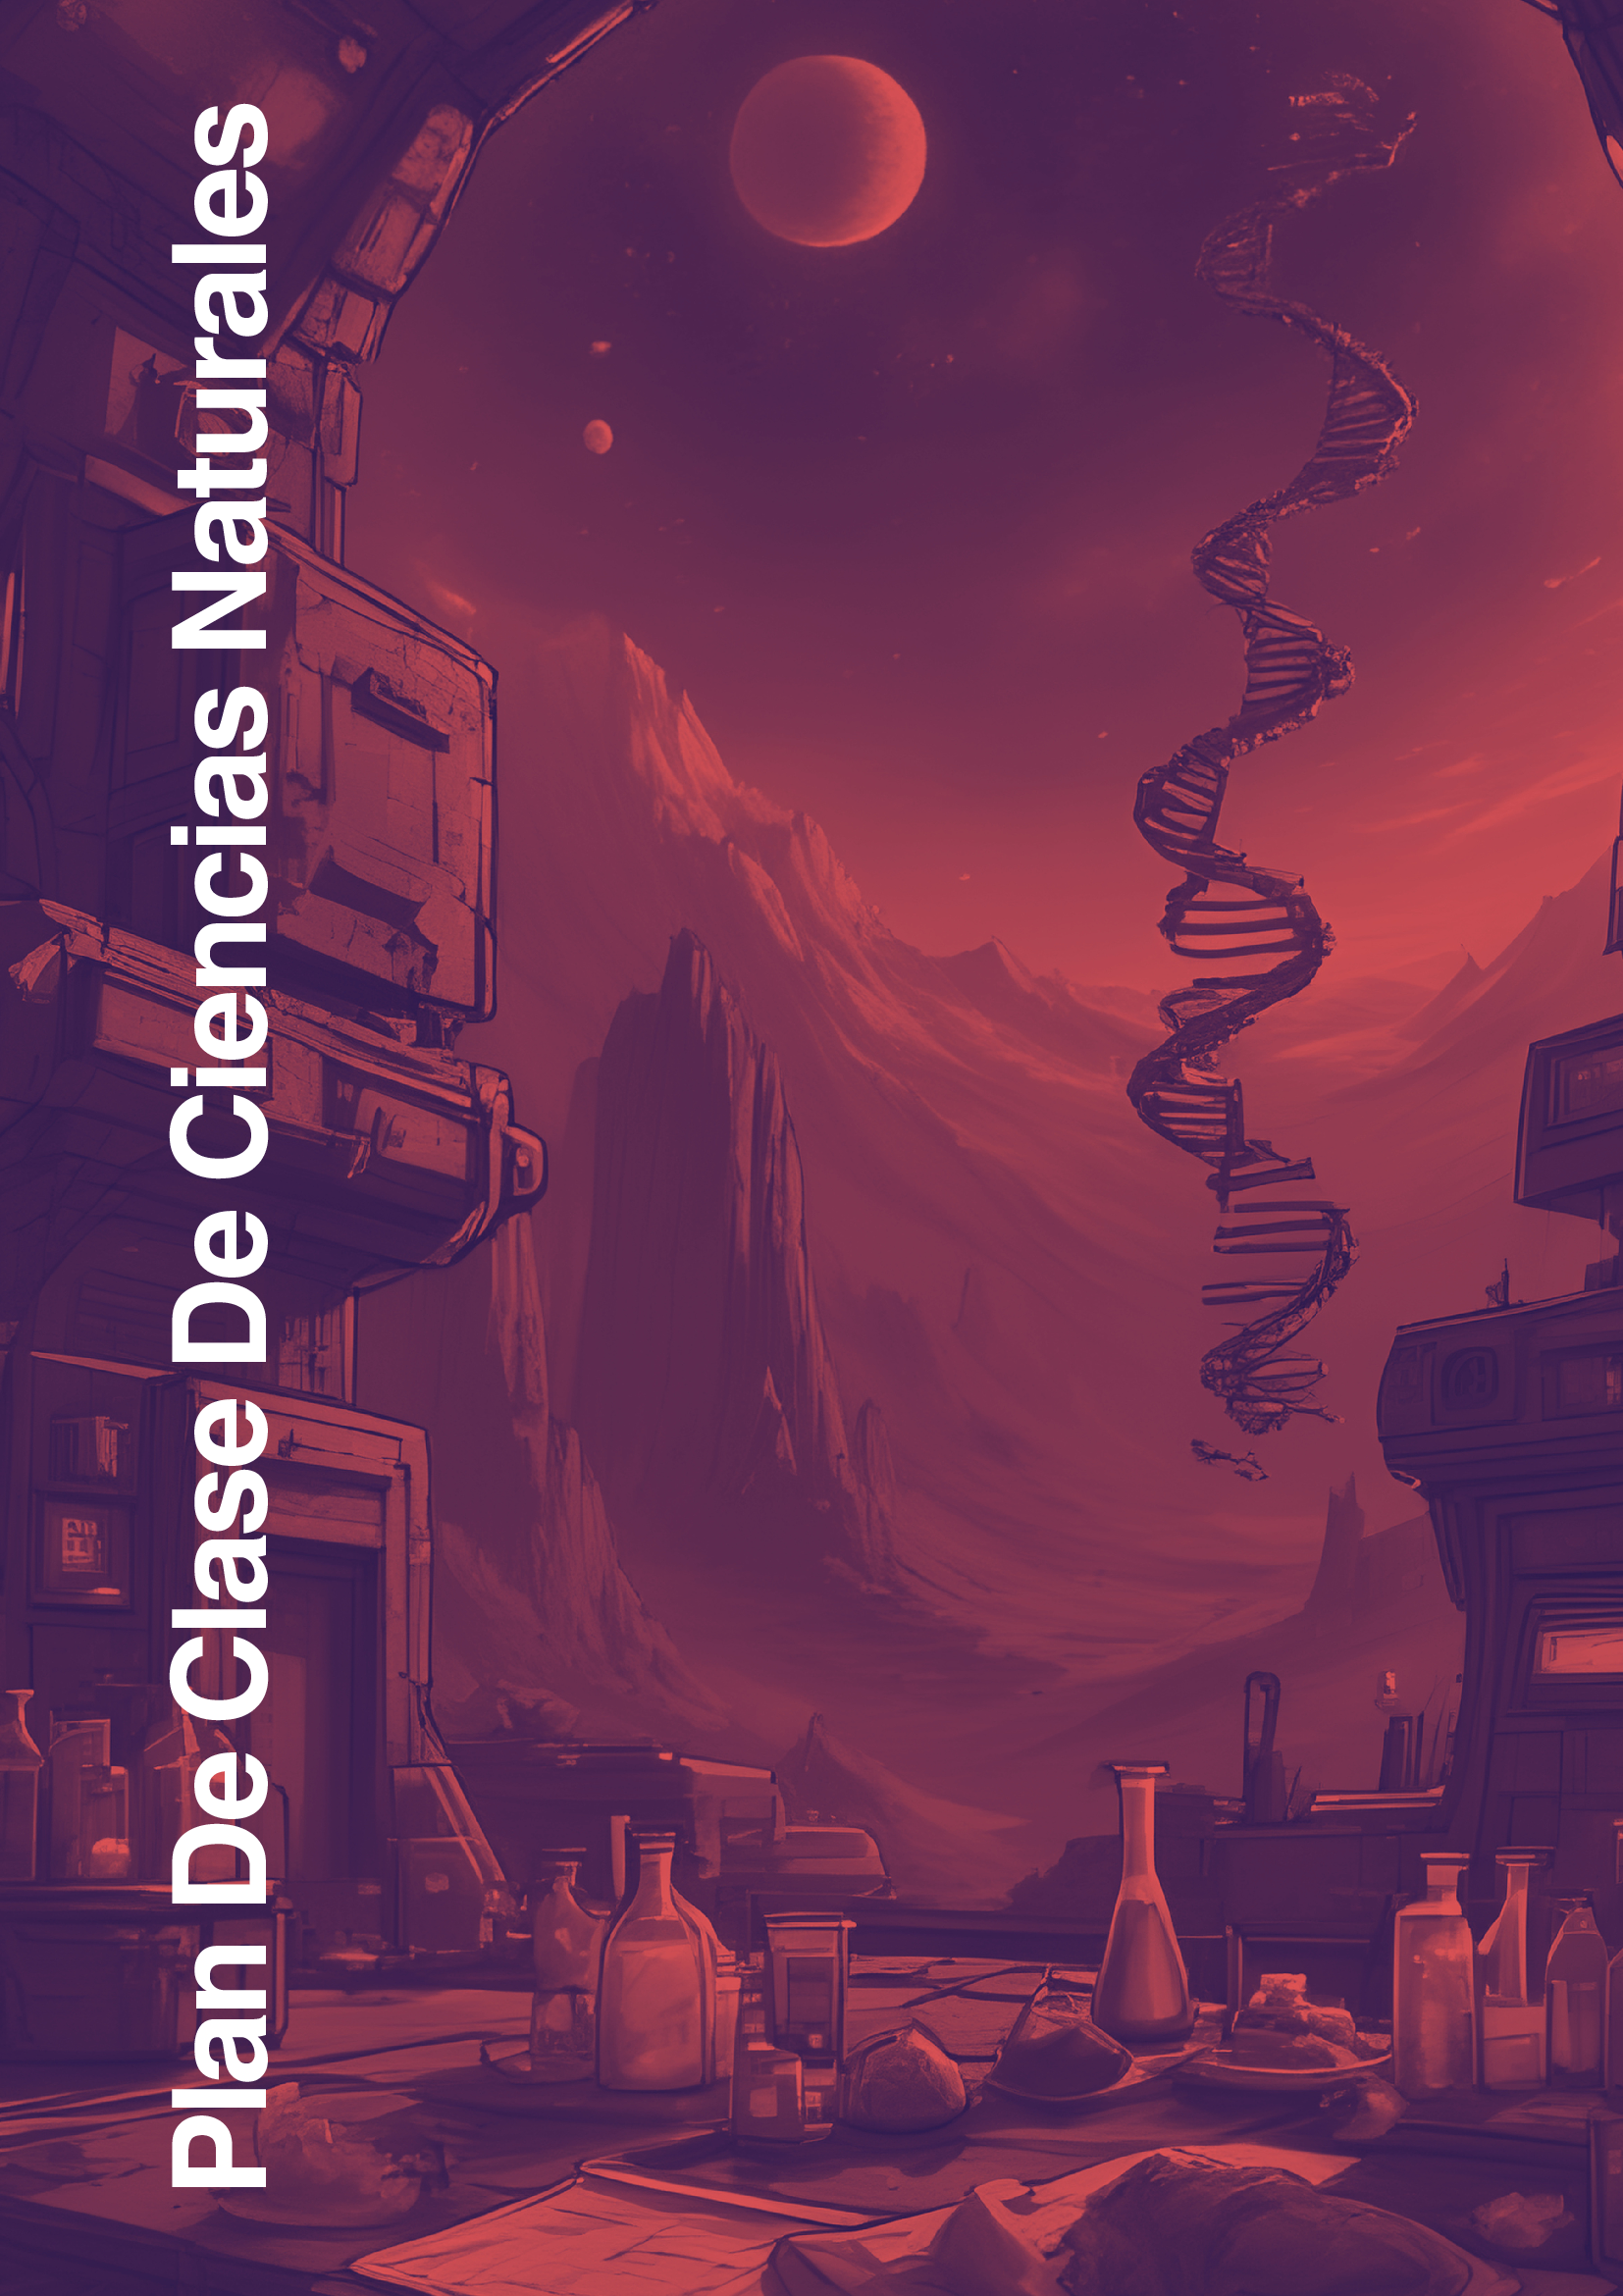
\includepdf[pages=-, fitpaper]{Portada.pdf}
  \mainmatter
  \pagestyle{plain}
}
\makeatletter
\@ifpackageloaded{tcolorbox}{}{\usepackage[skins,breakable]{tcolorbox}}
\@ifpackageloaded{fontawesome5}{}{\usepackage{fontawesome5}}
\definecolor{quarto-callout-color}{HTML}{909090}
\definecolor{quarto-callout-note-color}{HTML}{0758E5}
\definecolor{quarto-callout-important-color}{HTML}{CC1914}
\definecolor{quarto-callout-warning-color}{HTML}{EB9113}
\definecolor{quarto-callout-tip-color}{HTML}{00A047}
\definecolor{quarto-callout-caution-color}{HTML}{FC5300}
\definecolor{quarto-callout-color-frame}{HTML}{acacac}
\definecolor{quarto-callout-note-color-frame}{HTML}{4582ec}
\definecolor{quarto-callout-important-color-frame}{HTML}{d9534f}
\definecolor{quarto-callout-warning-color-frame}{HTML}{f0ad4e}
\definecolor{quarto-callout-tip-color-frame}{HTML}{02b875}
\definecolor{quarto-callout-caution-color-frame}{HTML}{fd7e14}
\makeatother
\makeatletter
\@ifpackageloaded{caption}{}{\usepackage{caption}}
\AtBeginDocument{%
\ifdefined\contentsname
  \renewcommand*\contentsname{Contenido}
\else
  \newcommand\contentsname{Contenido}
\fi
\ifdefined\listfigurename
  \renewcommand*\listfigurename{Listado de Figuras}
\else
  \newcommand\listfigurename{Listado de Figuras}
\fi
\ifdefined\listtablename
  \renewcommand*\listtablename{Listado de Tablas}
\else
  \newcommand\listtablename{Listado de Tablas}
\fi
\ifdefined\figurename
  \renewcommand*\figurename{Figura}
\else
  \newcommand\figurename{Figura}
\fi
\ifdefined\tablename
  \renewcommand*\tablename{Tabla}
\else
  \newcommand\tablename{Tabla}
\fi
}
\@ifpackageloaded{float}{}{\usepackage{float}}
\floatstyle{ruled}
\@ifundefined{c@chapter}{\newfloat{codelisting}{h}{lop}}{\newfloat{codelisting}{h}{lop}[chapter]}
\floatname{codelisting}{Listado}
\newcommand*\listoflistings{\listof{codelisting}{Listado de Listados}}
\makeatother
\makeatletter
\makeatother
\makeatletter
\@ifpackageloaded{caption}{}{\usepackage{caption}}
\@ifpackageloaded{subcaption}{}{\usepackage{subcaption}}
\makeatother
\makeatletter
\@ifpackageloaded{pdflscape}{}{\usepackage{pdflscape}}
\makeatother
\makeatletter
\@ifpackageloaded{colortbl}{}{\usepackage{colortbl}}
\makeatother
\usepackage{bookmark}
\IfFileExists{xurl.sty}{\usepackage{xurl}}{} % add URL line breaks if available
\urlstyle{same}
% fallback for those not using the hyperref driver hyperxmp:
\makeatletter
\@ifundefined{xmpquote}{\newcommand{\xmpquote}[1]{#1}}{}
\makeatother
\hypersetup{
  pdftitle={Natura Docens},
  pdflang={es},
  colorlinks=true,
  linkcolor={docere-link},
  filecolor={Maroon},
  citecolor={docere-cite},
  urlcolor={docere-url},
  pdfcreator={LaTeX via pandoc}}


\title{Natura Docens}
\author{}
\date{}
\begin{document}
\frontmatter
\maketitle

\renewcommand*\contentsname{Contenido}
{
\setcounter{tocdepth}{0}
\tableofcontents
}

\mainmatter
\chapter{Inicio}\label{inicio}

\textbf{Guía didáctica para grados 6° a 11° con enfoque pedagógico
inclusivo.}

Este libro reúne planes de clase estructurados con teoría, ideas
previas, contextualización, ejercicios, retos, aplicación y componente
socioemocional para cada tema del área de Ciencias Naturales.

\chapter{Estructura del libro}\label{estructura-del-libro}

Cada tema está organizado en las siguientes secciones:

\section{Detalles de la Estructura}\label{detalles-de-la-estructura}

\begin{itemize}
\tightlist
\item
  \textbf{Teoría} --- Contenido conceptual fundamental
\item
  \textbf{Ideas previas} --- Cuentos y preguntas para activar
  conocimientos
\item
  \textbf{Contextualización} --- Aplicación del método Richard Feynman
\item
  \textbf{Contextualización para caracterizados} --- Estrategias
  diferenciadas (cognitivo, TDAH, TEA, accesibilidad visual, motora)
\item
  \textbf{Ejemplo} --- Casos guiados en niveles básico, intermedio y
  avanzado
\item
  \textbf{Ejercicios} --- Práctica estructurada
\item
  \textbf{Retos} --- Problemas de profundización
\item
  \textbf{Aplicación} --- Conexión con la vida real y laboratorio
\item
  \textbf{Socioemocional} --- Acompañamiento emocional del aprendizaje
\end{itemize}

\part{Generalidades}

\chapter{Generalidades}\label{generalidades-1}

Este documento presenta un plan de temas por periodos para el
\textbf{área de Ciencias Naturales} (Biología, Física y Química),
dirigido a docentes, como guía de organización y secuenciación de
contenidos durante el año escolar.

\begin{tcolorbox}[enhanced jigsaw, arc=.35mm, bottomrule=.15mm, bottomtitle=1mm, breakable, colback=white, colbacktitle=quarto-callout-important-color!10!white, colframe=quarto-callout-important-color-frame, coltitle=black, left=2mm, leftrule=.75mm, opacityback=0, opacitybacktitle=0.6, rightrule=.15mm, title=\textcolor{quarto-callout-important-color}{\faExclamation}\hspace{0.5em}{Fundamentación}, titlerule=0mm, toprule=.15mm, toptitle=1mm]

En fundamentación se establece el contenido teórico específico y
concreto. Acá se establece la información respaldada por libros
universitarios, enfocada a la temática específica o artículos de
revisión o de investigación. El docente que quiera aportar en la forma
de explicar el concepto lo puede realizar en conceptualización.

\end{tcolorbox}

Este documento se actualiza de forma colaborativa. Para facilitar el
seguimiento, se recomienda registrar aquí quién realizó cada
modificación y qué se cambió (por ejemplo: correcciones de redacción,
incorporación de secciones, ajuste de figuras o referencias).

\begingroup
\arrayrulecolor{icfesborder}
{

\begin{longtable}[]{@{}lll@{}}

\caption{\label{tbl-registro-cambios}Registro de cambios}

\tabularnewline

\toprule\noalign{}
\rowcolor{icfesheader}\color{icfestext}\bfseries
Fecha & Usuario & Cambio realizado \\
\midrule\noalign{}
\endhead
\bottomrule\noalign{}
\endlastfoot
\rowcolors{2}{icfeveryodd}{icfeveryeven}
\color{icfestabletext}\mdseries
8-Jun-2026 & Camilo Tayac & Reactivo Limite \\

\end{longtable}

}\arrayrulecolor{black}
\endgroup

\section{Prefacio}\label{prefacio}

Este libro de Ciencias Naturales está diseñado para acompañar el proceso
de aprendizaje desde grado sexto hasta grado undécimo, integrando
Biología, Física y Química en una ruta progresiva. El material prioriza
la comprensión conceptual, el razonamiento científico y la aplicación
práctica de los contenidos en contextos escolares.

La organización de cada unidad busca mantener un equilibrio entre
precisión académica y lenguaje accesible. Por esa razón, los temas se
presentan de lo general a lo específico, con explicaciones
estructuradas, ejemplos guiados y actividades que fortalecen habilidades
cognitivas como análisis, interpretación y resolución de problemas.

El enfoque metodológico combina fundamentación teórica,
contextualización didáctica y ejercicios de consolidación. De este modo,
el texto puede utilizarse tanto en clase como en trabajo autónomo,
procesos de nivelación o preparación de evaluaciones.

\section{Cómo está organizado este
libro}\label{cuxf3mo-estuxe1-organizado-este-libro}

Cada bloque por grado incluye una secuencia de contenidos por periodos
académicos y por área. Dentro de cada tema, se mantiene una estructura
consistente para facilitar la lectura:

\begin{itemize}
\tightlist
\item
  presentación del concepto central,
\item
  desarrollo explicativo paso a paso,
\item
  ejemplos de aplicación,
\item
  actividades para fortalecer la comprensión.
\end{itemize}

\section{Sugerencias de uso}\label{sugerencias-de-uso}

Se recomienda trabajar los contenidos en orden, registrar ideas clave y
verificar la comprensión con los ejercicios propuestos. Cuando aparezcan
dificultades, conviene retomar los ejemplos y relacionarlos con
situaciones del entorno cotidiano.

\chapter{Plan de Área de Ciencias
Naturales}\label{plan-de-uxe1rea-de-ciencias-naturales}

\begin{quote}
\textbf{Intensidad horaria semanal por grado:}
\end{quote}

\begin{landscape}
\centering
\small
\begingroup
\arrayrulecolor{icfesborder}
{\def\LTcaptype{none} % do not increment counter
\begin{longtable*}[]{@{}
  >{\raggedright\arraybackslash}p{(\linewidth - 22\tabcolsep) * \real{0.0833}}
  >{\raggedright\arraybackslash}p{(\linewidth - 22\tabcolsep) * \real{0.0833}}
  >{\raggedright\arraybackslash}p{(\linewidth - 22\tabcolsep) * \real{0.0833}}
  >{\raggedright\arraybackslash}p{(\linewidth - 22\tabcolsep) * \real{0.0833}}
  >{\raggedright\arraybackslash}p{(\linewidth - 22\tabcolsep) * \real{0.0833}}
  >{\raggedright\arraybackslash}p{(\linewidth - 22\tabcolsep) * \real{0.0833}}
  >{\raggedright\arraybackslash}p{(\linewidth - 22\tabcolsep) * \real{0.0833}}
  >{\raggedright\arraybackslash}p{(\linewidth - 22\tabcolsep) * \real{0.0833}}
  >{\raggedright\arraybackslash}p{(\linewidth - 22\tabcolsep) * \real{0.0833}}
  >{\raggedright\arraybackslash}p{(\linewidth - 22\tabcolsep) * \real{0.0833}}
  >{\raggedright\arraybackslash}p{(\linewidth - 22\tabcolsep) * \real{0.0833}}
  >{\raggedright\arraybackslash}p{(\linewidth - 22\tabcolsep) * \real{0.0833}}@{}}
\toprule\noalign{}
\rowcolor{icfesheader}\color{icfestext}\bfseries
\begin{minipage}[b]{\linewidth}\raggedright
Asignatura
\end{minipage} & \begin{minipage}[b]{\linewidth}\raggedright
1°
\end{minipage} & \begin{minipage}[b]{\linewidth}\raggedright
2°
\end{minipage} & \begin{minipage}[b]{\linewidth}\raggedright
3°
\end{minipage} & \begin{minipage}[b]{\linewidth}\raggedright
4°
\end{minipage} & \begin{minipage}[b]{\linewidth}\raggedright
5°
\end{minipage} & \begin{minipage}[b]{\linewidth}\raggedright
6°
\end{minipage} & \begin{minipage}[b]{\linewidth}\raggedright
7°
\end{minipage} & \begin{minipage}[b]{\linewidth}\raggedright
8°
\end{minipage} & \begin{minipage}[b]{\linewidth}\raggedright
9°
\end{minipage} & \begin{minipage}[b]{\linewidth}\raggedright
10°
\end{minipage} & \begin{minipage}[b]{\linewidth}\raggedright
11°
\end{minipage} \\
\midrule\noalign{}
\endhead
\bottomrule\noalign{}
\endlastfoot
\rowcolors{2}{icfeveryodd}{icfeveryeven}
\color{icfestabletext}\mdseries
Ciencias Naturales (integrada) & 4 & 4 & 3 & 3 & 3 & --- & --- & --- &
--- & --- & --- \\
Biología & --- & --- & --- & --- & --- & 2 & 2 & 2 & 2 & 2 & 2 \\
Física & --- & --- & --- & --- & --- & 1 & 1 & 1 & 2 & 4 & 4 \\
Química & --- & --- & --- & --- & --- & 1 & 1 & 1 & 2 & 4 & 4 \\
\textbf{Total} & \textbf{4} & \textbf{4} & \textbf{3} & \textbf{3} &
\textbf{3} & \textbf{4} & \textbf{4} & \textbf{4} & \textbf{6} &
\textbf{10} & \textbf{10} \\
\end{longtable*}
}\arrayrulecolor{black}
\endgroup
\normalsize
\end{landscape}

\begin{center}\rule{0.5\linewidth}{0.5pt}\end{center}

\section{Primaria (Grados 1°-5°): Ciencias Naturales
Integradas}\label{primaria-grados-1-5-ciencias-naturales-integradas}

\begin{quote}
\textbf{Nota:} DBA = Derechos Básicos de Aprendizaje; Est. = Estándares
de Competencia; G = Guía; U = Unidad. \textbf{Libros:} BJ =
\emph{Biología: Juego y me comunico} (Grado 1); CN2 = \emph{Ciencias
Naturales y Educación Ambiental 2} (Grado 2); CN3 = \emph{Ciencias
Naturales y Educación Ambiental 3} (Grado 3); EA = \emph{Cartillas de
Escuela Activa} (Grados 4-5).
\end{quote}

\begin{landscape}
\centering
\small
\begingroup
\arrayrulecolor{icfesborder}
{\def\LTcaptype{none} % do not increment counter
\begin{longtable*}[]{@{}
  >{\raggedright\arraybackslash}p{(\linewidth - 12\tabcolsep) * \real{0.0500}}
  >{\raggedright\arraybackslash}p{(\linewidth - 12\tabcolsep) * \real{0.0500}}
  >{\raggedright\arraybackslash}p{(\linewidth - 12\tabcolsep) * \real{0.2000}}
  >{\raggedright\arraybackslash}p{(\linewidth - 12\tabcolsep) * \real{0.2000}}
  >{\raggedright\arraybackslash}p{(\linewidth - 12\tabcolsep) * \real{0.2000}}
  >{\raggedright\arraybackslash}p{(\linewidth - 12\tabcolsep) * \real{0.2000}}
  >{\raggedright\arraybackslash}p{(\linewidth - 12\tabcolsep) * \real{0.1000}}@{}}
\toprule\noalign{}
\rowcolor{icfesheader}\color{icfestext}\bfseries
\begin{minipage}[b]{\linewidth}\raggedright
G
\end{minipage} & \begin{minipage}[b]{\linewidth}\raggedright
P
\end{minipage} & \begin{minipage}[b]{\linewidth}\raggedright
Eje Temático
\end{minipage} & \begin{minipage}[b]{\linewidth}\raggedright
DBA
\end{minipage} & \begin{minipage}[b]{\linewidth}\raggedright
Estándares
\end{minipage} & \begin{minipage}[b]{\linewidth}\raggedright
Pre-req
\end{minipage} & \begin{minipage}[b]{\linewidth}\raggedright
Cap.
\end{minipage} \\
\midrule\noalign{}
\endhead
\bottomrule\noalign{}
\endlastfoot
\rowcolors{2}{icfeveryodd}{icfeveryeven}
\color{icfestabletext}\mdseries
1° & I & ¿Cómo son las personas que quiero y el lugar donde vivo? & DBA
5 (Sociales): Reconoce su individualidad y su pertenencia a los
diferentes grupos sociales. & --- & Distingue entre conocidos,
compañeros y personas que quiere. & BJ G 1-4 \\
1° & II & ¡Comuniquemos nuestras ideas! & DBA 8 (Lenguaje): Escribe
palabras que le permiten comunicar sus ideas, preferencias y
aprendizajes. & --- & Reconoce que lo que piensa o siente, tiene valor y
merece ser escuchado. & BJ G 5-9 \\
1° & III & ¡Hagamos preguntas! & DBA 7 (Lenguaje): Enuncia textos orales
de diferente índole sobre temas de su interés o sugeridos por otros. &
--- & Conoce la diferencia entre una frase afirmativa y una
interrogativa. & BJ G 10-14 \\
1° & IV & ¿Qué sabemos sobre los animales y las plantas? & DBA 3:
Comprende que los seres vivos (plantas y animales) tienen
características comunes (se alimentan, respiran, tienen un ciclo de
vida, responden al entorno) y los diferencia de los objetos inertes. &
Describo características de seres vivos y objetos inertes, establezco
semejanzas y diferencias entre ellos y los clasifico. (Est. 1°-3°,
Entorno vivo) & Diferencia claramente un animal o planta real de un
juguete. & BJ G 15-18 \\
& & & & & & \\
2° & I & Los seres vivos habitan en diferentes medios según sus
características & DBA 3: Comprende la relación entre las características
físicas de plantas y animales con los ambientes en donde viven, teniendo
en cuenta sus necesidades básicas (luz, agua, aire, suelo, nutrientes,
desplazamiento y protección). & Identifico y describo la flora, la
fauna, el agua y el suelo de mi entorno. / Describo características de
seres vivos y objetos inertes, establezco semejanzas y diferencias entre
ellos y los clasifico. (Est. 1°-3°, Entorno vivo) & Noción del ser vivo
vs.~ser inerte. & CN2 G 1-6 \\
2° & II & Los seres vivos se desarrollan y sufren cambios & DBA 4:
Explica los procesos de cambios físicos que ocurren en el ciclo de vida
de plantas y animales de su entorno, en un período de tiempo
determinado. & Propongo y verifico necesidades de los seres vivos. /
Reconozco que los hijos y las hijas se parecen a sus padres y describo
algunas características que se heredan. (Est. 1°-3°, Entorno vivo) &
Reconoce el ciclo vital de los seres vivos: nacer, crecer, reproducirse
y morir. & CN2 G 7-12 \\
2° & III & Estudiemos la energía, la fuerza y el movimiento & DBA 1
(Grado 1°): Comprende que una acción mecánica (fuerza) puede producir
distintas deformaciones en un objeto, y que este resiste a las fuerzas
de diferente modo, de acuerdo con el material del que está hecho. &
Reconozco en el entorno fenómenos físicos que me afectan y desarrollo
habilidades para aproximarme a ellos. (Est. 1°-3°, Entorno físico) &
Noción de cuerpo, objeto y materia, además la posición, localización y
fuentes de energía. & CN2 G 13-18 \\
2° & IV & Estudiemos la materia y sus propiedades & DBA 2 (Grado 1°):
Comprende que las sustancias pueden encontrarse en distintos estados
(sólido, líquido y gaseoso). & Clasifico y comparo objetos según sus
usos. / Diferencio objetos naturales de objetos creados por el ser
humano. (Est. 1°-3°, Entorno físico) & Identifica los estados físicos de
la naturaleza. & CN2 G 19-24 \\
& & & & & & \\
3° & I & ¿Cómo son los seres de mi entorno? & DBA 3 (Grado 1°):
Comprende que los seres vivos (plantas y animales) tienen
características comunes (se alimentan, respiran, tienen un ciclo de
vida, responden al entorno) y los diferencia de los objetos inertes. &
Describo características de seres vivos y objetos inertes, establezco
semejanzas y diferencias entre ellos y los clasifico. (Est. 1°-3°,
Entorno vivo) & Diferenciación entre seres vivos y objetos inertes
(Grado 2°). & CN3 G 1-4 \\
3° & II & ¿Dónde viven y cómo se adaptan los seres vivos? & DBA 5:
Explica la influencia de los factores abióticos (luz, temperatura, suelo
y aire) en el desarrollo de los factores bióticos (fauna y flora) de un
ecosistema. & Diferencio tipos de plantas y animales según sus
estructuras externas y sus respuestas de adaptación al medio ambiente. /
Explico la dinámica de un ecosistema considerando las necesidades de
energía y nutrientes de sus seres vivos. (Est. 1°-3°, Entorno vivo) &
Noción de ciclo de vida y necesidades básicas de los seres vivos (Grado
2°). & CN3 G 5-8 \\
3° & III & ¿De qué están hechas las cosas? & DBA 4: Comprende la
influencia de la variación de la temperatura en los cambios de estado de
la materia, considerando como ejemplo el caso del agua. & Reconozco que
los objetos y la materia que me rodea tienen propiedades particulares y
cambian ante ciertos estímulos. / Clasifico materiales de uso cotidiano
de acuerdo con sus propiedades físicas y su utilidad. (Est. 1°-3°,
Entorno físico) & Identificación de propiedades de la materia y sus
estados (Grado 2°). & CN3 G 9-12 \\
3° & IV & ¿Por qué se mueven y cambian las cosas? & DBA 1: Comprende que
la magnitud y la dirección en que se aplica una fuerza puede producir
cambios en la forma como se mueve un objeto (dirección y rapidez). &
Identifico tipos de fuerza que actúan sobre los objetos y su capacidad
para modificar el movimiento de los cuerpos. / Reconozco el Sol como la
fuente fundamental de luz y calor, y su relevancia para la vida. (Est.
1°-3°, Entorno físico y CTS) & Noción de fuerza, movimiento y energía
(Grado 2°). & CN3 G 13-16 \\
& & & & & & \\
4° & I & El Universo y el Sistema Solar. & DBA 6 (Grado 4°): Comprende
que el Sistema Solar está compuesto por el Sol, los planetas y otros
cuerpos celestes, y que la Tierra realiza movimientos que determinan la
duración del día, la noche y las estaciones del año. & Reconozco
características de los cuerpos celestes que integran nuestro Sistema
Solar y establezco relaciones con las condiciones de vida en la Tierra.
(Est. 4°-5°, Entorno Físico / CTS) & Noción de día, noche y estaciones
(Grado 3°). & EA U 1 \\
4° & II & Ecosistemas, relaciones y flujo de energía. & DBA 1 (Grado
4°): Analiza las relaciones que se establecen entre las poblaciones de
un ecosistema (competencia, mutualismo, parasitismo, depredación) y el
flujo de energía a través de redes tróficas. & Identifico adaptaciones
de los seres vivos para preservar el equilibrio en los ecosistemas y
represento estas relaciones mediante cadenas alimenticias. (Est. 4°-5°,
Entorno Vivo) & Factores bióticos y abióticos (Grado 3°). & EA U 2 \\
4° & III & Sustancias químicas y propiedades de la materia. & DBA 2
(Grado 4°): Comprende que existen distintos tipos de mezclas (homogéneas
y heterogéneas) que se pueden separar utilizando diferentes métodos
físicos. & Verifico de forma práctica y experimental diferentes métodos
de separación de mezclas. (Est. 4°-5°, Entorno Físico) & Propiedades
generales de la materia (Grado 3°). & EA U 3 \\
4° & IV & Las fuerzas y el movimiento. & DBA 5 (Grado 4°): Comprende los
efectos de la fuerza de gravedad y la fuerza de fricción en el
movimiento de los cuerpos, y cómo el diseño de máquinas simples facilita
y optimiza el trabajo humano. & Identifico la utilidad e historia de las
máquinas simples y las aplico de manera dirigida para resolver
problemas. (Est. 4°-5°, Entorno Físico / CTS) & Noción de fuerza y
movimiento (Grado 3°). & EA U 4 \\
& & & & & & \\
5° & I & Organización interna de los seres vivos: célula y tejidos. &
DBA 3 (Grado 5°): Comprende que los sistemas de órganos en los seres
vivos se componen de tejidos de células especializadas que cooperan en
la ejecución de funciones vitales y metabólicas complejas. & Explico la
estructura y función de la célula como unidad biológica básica y su
organización en tejidos diferenciados. (Est. 4°-5°, Entorno Vivo) &
Características de los seres vivos y su clasificación (Grado 3°). & EA U
1 \\
5° & II & Sistemas y aparatos del ser humano. & DBA 4 (Grado 5°):
Comprende el camino que siguen los alimentos en el organismo y los
cambios que sufren durante el proceso de digestión, así como la
interrelación obligatoria con los sistemas circulatorio y respiratorio.
& Represento e identifico los principales sistemas de órganos del ser
humano y explico sus funciones e interdependencias vitales. (Est. 4°-5°,
Entorno Vivo) & Organización celular y tejidos (Periodo 1). & EA U 2 \\
5° & III & Sustancias químicas y sus propiedades. & DBA 2 (Grado 5°):
Comprende que la materia está formada por partículas y que las
propiedades específicas de las sustancias permiten diferenciar elementos
de compuestos, así como transformaciones químicas de las físicas. &
Diferencio los cambios físicos de los químicos en objetos del entorno.
(Est. 4°-5°, Entorno Físico) & Mezclas y métodos de separación (Grado
4°). & EA U 3 \\
5° & IV & La electricidad y sus funciones en la vida diaria. & DBA 5
(Grado 5°): Comprende que la energía eléctrica puede transitar a través
de canales conductores dentro de un circuito cerrado y transformarse en
otros tipos de energía. & Construyo circuitos eléctricos simples
funcionales utilizando diferentes materiales conductores y aislantes.
(Est. 4°-5°, Entorno Físico / CTS) & Fuerzas, movimiento y energía
(Grado 4°). & EA U 4 \\
& & & & & & \\
\end{longtable*}
}\arrayrulecolor{black}
\endgroup
\normalsize
\end{landscape}

\begin{center}\rule{0.5\linewidth}{0.5pt}\end{center}

\section{Biología (Grados 6°-7°)}\label{biologuxeda-grados-6-7}

\begin{quote}
\textbf{Nota:} Est. = Estándares de Competencias; Cap. = Capítulo.
\textbf{Libro de texto:} B = \emph{Biología: la vida en la Tierra con
Fisiología} (Audesirk, Audesirk \& Byers, 10ª ed., 2017).
\textbf{Nivel:} Exploratorio (1°-3°) → Diferencial (4°-5°, 6°-9°) →
Disciplinar (10°-11°).
\end{quote}

\begin{landscape}
\centering
\small
\begingroup
\arrayrulecolor{icfesborder}
{\def\LTcaptype{none} % do not increment counter
\begin{longtable*}[]{@{}
  >{\raggedright\arraybackslash}p{(\linewidth - 10\tabcolsep) * \real{0.1667}}
  >{\raggedright\arraybackslash}p{(\linewidth - 10\tabcolsep) * \real{0.1667}}
  >{\raggedright\arraybackslash}p{(\linewidth - 10\tabcolsep) * \real{0.1667}}
  >{\raggedright\arraybackslash}p{(\linewidth - 10\tabcolsep) * \real{0.1667}}
  >{\raggedright\arraybackslash}p{(\linewidth - 10\tabcolsep) * \real{0.1667}}
  >{\raggedright\arraybackslash}p{(\linewidth - 10\tabcolsep) * \real{0.1667}}@{}}
\toprule\noalign{}
\rowcolor{icfesheader}\color{icfestext}\bfseries
\begin{minipage}[b]{\linewidth}\raggedright
G
\end{minipage} & \begin{minipage}[b]{\linewidth}\raggedright
P
\end{minipage} & \begin{minipage}[b]{\linewidth}\raggedright
Eje Temático
\end{minipage} & \begin{minipage}[b]{\linewidth}\raggedright
Estándares
\end{minipage} & \begin{minipage}[b]{\linewidth}\raggedright
Pre-req
\end{minipage} & \begin{minipage}[b]{\linewidth}\raggedright
Cap. B
\end{minipage} \\
\midrule\noalign{}
\endhead
\bottomrule\noalign{}
\endlastfoot
\rowcolors{2}{icfeveryodd}{icfeveryeven}
\color{icfestabletext}\mdseries
6° & I & \textbf{La célula y las moléculas de la vida.} Características
de los seres vivos. Átomos y moléculas. Biomoléculas: carbohidratos,
lípidos, proteínas y ácidos nucleicos. Teoría celular. Célula procariota
y eucariota. Organelos y sus funciones. & Explico la estructura de la
célula y las funciones básicas de sus componentes. (Est. 6°-7°, Entorno
vivo) & Organización interna de los seres vivos: célula y tejidos (Grado
5°). & B 1-4 \\
6° & II & \textbf{La membrana celular y el transporte de sustancias.}
Estructura de la membrana: modelo del mosaico fluido. Permeabilidad
selectiva. Difusión y ósmosis. Transporte pasivo y activo. Endocitosis y
exocitosis. & Verifico y explico los procesos de ósmosis y difusión.
Clasifico membranas de los seres vivos de acuerdo con su permeabilidad
frente a diversas sustancias. (Est. 6°-7°, Entorno vivo) & La célula y
las moléculas de la vida (Período I). & B 5 \\
6° & III & \textbf{Sistemas del cuerpo humano.} Sistemas digestivo,
respiratorio y circulatorio. Nutrición y salud. Relación entre
estructura y función a nivel de sistemas de órganos. Comparación de
estos sistemas con los de otros vertebrados. & Comparo sistemas de
órganos de diferentes grupos taxonómicos. (Est. 6°-7°, Entorno vivo) &
La célula y las moléculas de la vida (Período I) y la membrana celular y
el transporte de sustancias (Período II). & B 32-34 \\
6° & IV & \textbf{Clasificación de los seres vivos.} Criterios de
clasificación. Dominios y reinos. Taxonomía básica: especie, género,
familia, orden, clase, filo, reino. Diversidad: procariontes, virus,
protistas, hongos y plantas. & Clasifico organismos en grupos
taxonómicos de acuerdo con las características de sus células. (Est.
6°-7°, Entorno vivo) & La célula y las moléculas de la vida (Período I).
& B 18-22 \\
& & & & & \\
7° & I & \textbf{División celular: mitosis y meiosis.} Ciclo celular.
Fases de la mitosis. Meiosis. Comparación entre mitosis y meiosis.
Importancia en el crecimiento, la reparación y la reproducción. &
Comparo sistemas de división celular y argumento su importancia en la
generación de nuevos organismos y tejidos. (Est. 6°-7°, Entorno vivo) &
La célula y las moléculas de la vida (Grado 6°). & B 9 \\
7° & II & \textbf{Origen del universo y de la vida.} Teorías sobre el
origen del universo. Teorías del origen de la vida: generación
espontánea, panspermia y evolución química. Primeras formas de vida. &
Explico el origen del universo y de la vida a partir de varias teorías.
(Est. 6°-7°, Entorno vivo) & La célula y las moléculas de la vida (Grado
6°). & B 17 + material complementario \\
7° & III & \textbf{Energía y ciclos de la materia en los ecosistemas.}
Fotosíntesis y respiración celular (nivel descriptivo). Flujo de
energía. Ciclos del agua, del carbono y del nitrógeno. El agua en el
sostenimiento de la vida. El suelo como depósito de nutrientes. &
Justifico la importancia del agua en el sostenimiento de la vida.
Describo y relaciono los ciclos del agua, de algunos elementos y de la
energía en los ecosistemas. Explico la función del suelo como depósito
de nutrientes. (Est. 6°-7°, Entorno vivo) & Ecosistemas, relaciones y
flujo de energía (Grado 4°). & B 6-8, 28 \\
7° & IV & \textbf{Biodiversidad, adaptación y conservación.} Ecosistemas
de Colombia y equilibrio dinámico de sus poblaciones. Adaptaciones de
los seres vivos. Causas de extinción. Estrategias de conservación.
Recursos naturales renovables y no renovables. & Evalúo el potencial de
los recursos naturales, la forma como se han utilizado en desarrollos
tecnológicos y las consecuencias de la acción del ser humano sobre
ellos. (Est. 6°-7°, CTS) & Energía y ciclos de la materia en los
ecosistemas (Período III). & B 27, 29-30 \\
& & & & & \\
\end{longtable*}
}\arrayrulecolor{black}
\endgroup
\normalsize
\end{landscape}

\begin{center}\rule{0.5\linewidth}{0.5pt}\end{center}

\section{Biología (Grados 8°-9°)}\label{biologuxeda-grados-8-9}

\begin{quote}
\textbf{Nota:} Est. = Estándares de Competencias; Cap. = Capítulo.
\textbf{Libro de texto:} B = \emph{Biología: la vida en la Tierra con
Fisiología} (Audesirk, Audesirk \& Byers, 10ª ed., 2017).
\textbf{Nivel:} Exploratorio (1°-3°) → Diferencial (4°-5°, 6°-9°) →
Disciplinar (10°-11°).
\end{quote}

\begin{landscape}
\centering
\small
\begingroup
\arrayrulecolor{icfesborder}
{\def\LTcaptype{none} % do not increment counter
\begin{longtable*}[]{@{}
  >{\raggedright\arraybackslash}p{(\linewidth - 10\tabcolsep) * \real{0.1667}}
  >{\raggedright\arraybackslash}p{(\linewidth - 10\tabcolsep) * \real{0.1667}}
  >{\raggedright\arraybackslash}p{(\linewidth - 10\tabcolsep) * \real{0.1667}}
  >{\raggedright\arraybackslash}p{(\linewidth - 10\tabcolsep) * \real{0.1667}}
  >{\raggedright\arraybackslash}p{(\linewidth - 10\tabcolsep) * \real{0.1667}}
  >{\raggedright\arraybackslash}p{(\linewidth - 10\tabcolsep) * \real{0.1667}}@{}}
\toprule\noalign{}
\rowcolor{icfesheader}\color{icfestext}\bfseries
\begin{minipage}[b]{\linewidth}\raggedright
G
\end{minipage} & \begin{minipage}[b]{\linewidth}\raggedright
P
\end{minipage} & \begin{minipage}[b]{\linewidth}\raggedright
Eje Temático
\end{minipage} & \begin{minipage}[b]{\linewidth}\raggedright
Estándares
\end{minipage} & \begin{minipage}[b]{\linewidth}\raggedright
Pre-req
\end{minipage} & \begin{minipage}[b]{\linewidth}\raggedright
Cap. B
\end{minipage} \\
\midrule\noalign{}
\endhead
\bottomrule\noalign{}
\endlastfoot
\rowcolors{2}{icfeveryodd}{icfeveryeven}
\color{icfestabletext}\mdseries
8° & I & \textbf{Herencia y estructura del ADN.} Patrones de herencia de
Mendel. Genotipo y fenotipo. Cuadrados de Punnett. Cromosomas. Modelo de
la doble hélice del ADN. Replicación y transmisión del material
hereditario. & Reconozco la importancia del modelo de la doble hélice
para la explicación del almacenamiento y transmisión del material
hereditario. (Est. 8°-9°, Entorno vivo) & División celular: mitosis y
meiosis (Período I, Grado 7°). & B 10-11 \\
8° & II & \textbf{Expresión génica y biotecnología.} Código genético.
Transcripción y traducción. Regulación de la expresión génica.
Mutaciones. Biotecnología: ADN recombinante, PCR, organismos
transgénicos. Implicaciones bioéticas. & Establezco relaciones entre los
genes, las proteínas y las funciones celulares. Reconozco la importancia
de las proteínas en el desarrollo de los seres vivos. (Est. 8°-9°,
Entorno vivo) & Herencia y estructura del ADN (Período I). & B 12-13 \\
8° & III & \textbf{Reproducción y variabilidad genética.} Reproducción
asexual y sexual. Meiosis. Comparación de sistemas de reproducción en
distintos grupos de seres vivos. Importancia de la reproducción sexual
en el mantenimiento de la variabilidad. & Comparo diferentes sistemas de
reproducción. Justifico la importancia de la reproducción sexual en el
mantenimiento de la variabilidad. (Est. 8°-9°, Entorno vivo) & División
celular: mitosis y meiosis (Período I, Grado 7°). & B 9, 41, 44 \\
8° & IV & \textbf{Reproducción humana y control de la natalidad.}
Sistema reproductor humano. Ciclo menstrual. Fecundación y desarrollo
embrionario. Métodos anticonceptivos. Control de la natalidad y dinámica
poblacional. Infecciones de transmisión sexual. & Establezco la relación
entre el ciclo menstrual y la reproducción humana. Analizo las
consecuencias del control de la natalidad en las poblaciones. Identifico
aplicaciones de algunos conocimientos sobre la herencia y la
reproducción al mejoramiento de la calidad de vida de las poblaciones.
(Est. 8°-9°, Entorno vivo / CTS) & Reproducción y variabilidad genética
(Período III). & B 41-42 \\
& & & & & \\
9° & I & \textbf{Diversidad animal y sistemas de órganos.}
Invertebrados: poríferos, cnidarios, moluscos y artrópodos. Vertebrados:
peces, anfibios, reptiles, aves y mamíferos. Comparación de sistemas de
órganos entre grupos taxonómicos. & Comparo sistemas de órganos de
diferentes grupos taxonómicos. (Est. 8°-9°, Entorno vivo) &
Clasificación de los seres vivos (Período IV, Grado 6°). & B 23-24 \\
9° & II & \textbf{Evolución: teorías sobre el origen de las especies.}
Desarrollo del pensamiento evolutivo. Darwin y Wallace: selección
natural. Evidencias de la evolución. Comparación de teorías sobre el
origen de las especies. Hipótesis sobre el origen y la evolución de
grupos de organismos. & Comparo diferentes teorías sobre el origen de
las especies. Formulo hipótesis acerca del origen y evolución de un
grupo de organismos. (Est. 8°-9°, Entorno vivo) & Herencia y estructura
del ADN (Grado 8°) y origen del universo y de la vida (Período II, Grado
7°). & B 14-16 \\
9° & III & \textbf{Historia de la vida y eras geológicas.} Fósiles y
datación. Eras geológicas. Relación entre el clima y las adaptaciones de
los seres vivos. Extinciones masivas. Evolución humana. & Establezco
relaciones entre el clima en las diferentes eras geológicas y las
adaptaciones de los seres vivos. (Est. 8°-9°, Entorno vivo) & Evolución:
teorías sobre el origen de las especies (Período II). & B 17 \\
9° & IV & \textbf{Regulación hormonal y sistemas de defensa.} Hormonas y
regulación de las funciones en el ser humano. Sistemas de defensa y
ataque de animales y plantas. & Explico la importancia de las hormonas
en la regulación de las funciones en el ser humano. Comparo y explico
los sistemas de defensa y ataque de algunos animales y plantas en el
aspecto morfológico y fisiológico. (Est. 8°-9°, Entorno vivo) &
Diversidad animal y sistemas de órganos (Período I). & B 36-37 \\
& & & & & \\
\end{longtable*}
}\arrayrulecolor{black}
\endgroup
\normalsize
\end{landscape}

\begin{center}\rule{0.5\linewidth}{0.5pt}\end{center}

\section{Biología (Grados 10°-11°)}\label{biologuxeda-grados-10-11}

\begin{quote}
\textbf{Nota:} Est. = Estándares de Competencias; Cap. = Capítulo.
\textbf{Libro de texto:} B = \emph{Biología: la vida en la Tierra con
Fisiología} (Audesirk, Audesirk \& Byers, 10ª ed., 2017).
\textbf{Nivel:} Exploratorio (1°-3°) → Diferencial (4°-5°, 6°-9°) →
Disciplinar (10°-11°).
\end{quote}

\begin{landscape}
\centering
\small
\begingroup
\arrayrulecolor{icfesborder}
{\def\LTcaptype{none} % do not increment counter
\begin{longtable*}[]{@{}
  >{\raggedright\arraybackslash}p{(\linewidth - 10\tabcolsep) * \real{0.1667}}
  >{\raggedright\arraybackslash}p{(\linewidth - 10\tabcolsep) * \real{0.1667}}
  >{\raggedright\arraybackslash}p{(\linewidth - 10\tabcolsep) * \real{0.1667}}
  >{\raggedright\arraybackslash}p{(\linewidth - 10\tabcolsep) * \real{0.1667}}
  >{\raggedright\arraybackslash}p{(\linewidth - 10\tabcolsep) * \real{0.1667}}
  >{\raggedright\arraybackslash}p{(\linewidth - 10\tabcolsep) * \real{0.1667}}@{}}
\toprule\noalign{}
\rowcolor{icfesheader}\color{icfestext}\bfseries
\begin{minipage}[b]{\linewidth}\raggedright
G
\end{minipage} & \begin{minipage}[b]{\linewidth}\raggedright
P
\end{minipage} & \begin{minipage}[b]{\linewidth}\raggedright
Eje Temático
\end{minipage} & \begin{minipage}[b]{\linewidth}\raggedright
Estándares
\end{minipage} & \begin{minipage}[b]{\linewidth}\raggedright
Pre-req
\end{minipage} & \begin{minipage}[b]{\linewidth}\raggedright
Cap. B
\end{minipage} \\
\midrule\noalign{}
\endhead
\bottomrule\noalign{}
\endlastfoot
\rowcolors{2}{icfeveryodd}{icfeveryeven}
\color{icfestabletext}\mdseries
10° & I & \textbf{Genética de poblaciones y evolución.} Genética de
poblaciones: ley de Hardy-Weinberg. Relación entre mutación, selección
natural y herencia. Casos en especies actuales que ilustran la selección
natural. & Establezco relaciones entre mutación, selección natural y
herencia. Comparo casos en especies actuales que ilustren diferentes
acciones de la selección natural. (Est. 10°-11°, Procesos biológicos) &
Herencia y estructura del ADN y evolución: teorías sobre el origen de
las especies (Grados 8°-9°). & B 14-16 \\
10° & II & \textbf{Fisiología animal: fluidos y señales.} Homeostasis.
Mecánica de fluidos en los seres vivos: sistema circulatorio. Neuronas y
señales eléctricas y químicas. Sistema nervioso y sentidos. & Identifico
y explico ejemplos del modelo de mecánica de fluidos en los seres vivos.
Explico el funcionamiento de neuronas a partir de modelos químicos y
eléctricos. (Est. 10°-11°, Procesos biológicos) & Diversidad animal y
sistemas de órganos (Período I, Grado 9°). & B 32, 38-39 \\
10° & III & \textbf{Energía en los ecosistemas.} Cadenas y redes
alimentarias. Relaciones entre materia y energía. Principios
termodinámicos en los ecosistemas. Productividad primaria. & Explico las
relaciones entre materia y energía en las cadenas alimentarias. Busco
ejemplos de principios termodinámicos en algunos ecosistemas. (Est.
10°-11°, Procesos biológicos) & Energía y ciclos de la materia en los
ecosistemas (Período III, Grado 7°). & B 6-8, 28 \\
10° & IV & \textbf{Ecología de poblaciones y comunidades.} Relaciones
entre individuo, población, comunidad y ecosistema. Crecimiento y
regulación de poblaciones. Relaciones entre especies. Sucesión
ecológica. & Establezco relaciones entre individuo, población, comunidad
y ecosistema. Explico diversos tipos de relaciones entre especies en los
ecosistemas. (Est. 10°-11°, Procesos biológicos) & Energía en los
ecosistemas (Período III). & B 26-27 \\
& & & & & \\
11° & I & \textbf{Ciclos biogeoquímicos y problemas ambientales
globales.} Ciclos del agua y de los elementos. Energía de los
ecosistemas. Cambio climático y contaminación como alteraciones de los
ciclos. & Relaciono los ciclos del agua y de los elementos con la
energía de los ecosistemas. (Est. 10°-11°, Procesos biológicos / CTS) &
Energía en los ecosistemas y ecología de poblaciones (Períodos III-IV,
Grado 10°). & B 28, 30 \\
11° & II & \textbf{Biodiversidad del mundo y de Colombia.} Biomas
terrestres y acuáticos. Adaptaciones de los seres vivos en ecosistemas
del mundo y de Colombia. Especies amenazadas. Conservación y áreas
protegidas. & Explico y comparo algunas adaptaciones de seres vivos en
ecosistemas del mundo y de Colombia. (Est. 10°-11°, Procesos biológicos)
& Ecología de poblaciones y comunidades (Período IV, Grado 10°). & B
29-30 \\
11° & III & \textbf{Fisiología vegetal.} Fotosíntesis como conversión de
energía. Transporte de agua y nutrientes: xilema y floema. Hormonas
vegetales. Fotoperiodismo. Respuestas de las plantas al ambiente. &
Argumento la importancia de la fotosíntesis como un proceso de
conversión de energía necesaria para organismos aerobios. (Est. 10°-11°,
Procesos biológicos) & Energía en los ecosistemas (Período III, Grado
10°). & B 7, 43, 45 \\
11° & IV & \textbf{Biotecnología avanzada y bioética.} Edición genómica:
CRISPR. Terapias génicas. Organismos transgénicos. Clonación. Relación
entre el ADN, el ambiente y la diversidad de los seres vivos. Debate
bioético. & Explico la relación entre el ADN, el ambiente y la
diversidad de los seres vivos. (Est. 10°-11°, Procesos biológicos / CTS)
& Expresión génica y biotecnología (Período II, Grado 8°). & B 13 \\
& & & & & \\
\end{longtable*}
}\arrayrulecolor{black}
\endgroup
\normalsize
\end{landscape}

\begin{center}\rule{0.5\linewidth}{0.5pt}\end{center}

\section{Química (Grados 6°-7°)}\label{quuxedmica-grados-6-7}

\begin{quote}
\textbf{Nota:} Est. = Estándares de Competencias; Cap. = Capítulo.
\textbf{Libro de texto:} Q = \emph{Química: La Ciencia Central} (Brown,
LeMay, Bursten, Murphy \& Woodward, 12ª ed., 2012). \textbf{Nivel:}
Exploratorio (1°-3°) → Diferencial (4°-5°, 6°-9°) → Disciplinar
(10°-11°).
\end{quote}

\begin{landscape}
\centering
\small
\begingroup
\arrayrulecolor{icfesborder}
{\def\LTcaptype{none} % do not increment counter
\begin{longtable*}[]{@{}
  >{\raggedright\arraybackslash}p{(\linewidth - 10\tabcolsep) * \real{0.1667}}
  >{\raggedright\arraybackslash}p{(\linewidth - 10\tabcolsep) * \real{0.1667}}
  >{\raggedright\arraybackslash}p{(\linewidth - 10\tabcolsep) * \real{0.1667}}
  >{\raggedright\arraybackslash}p{(\linewidth - 10\tabcolsep) * \real{0.1667}}
  >{\raggedright\arraybackslash}p{(\linewidth - 10\tabcolsep) * \real{0.1667}}
  >{\raggedright\arraybackslash}p{(\linewidth - 10\tabcolsep) * \real{0.1667}}@{}}
\toprule\noalign{}
\rowcolor{icfesheader}\color{icfestext}\bfseries
\begin{minipage}[b]{\linewidth}\raggedright
G
\end{minipage} & \begin{minipage}[b]{\linewidth}\raggedright
P
\end{minipage} & \begin{minipage}[b]{\linewidth}\raggedright
Eje Temático
\end{minipage} & \begin{minipage}[b]{\linewidth}\raggedright
Estándares
\end{minipage} & \begin{minipage}[b]{\linewidth}\raggedright
Pre-req
\end{minipage} & \begin{minipage}[b]{\linewidth}\raggedright
Cap. Q
\end{minipage} \\
\midrule\noalign{}
\endhead
\bottomrule\noalign{}
\endlastfoot
\rowcolors{2}{icfeveryodd}{icfeveryeven}
\color{icfestabletext}\mdseries
6° & I & \textbf{Estados de la materia y cambios de estado.} Sólido,
líquido, gaseoso y plasma. Cambios de estado: fusión, solidificación,
evaporación, condensación, sublimación. Energía y cambios de estado. &
Clasifico y verifico las propiedades de la materia. (Est. 6°-7°, Entorno
físico) & Propiedades de la materia y sus estados (Grado 3°). & Q 1 \\
6° & II & \textbf{Mezclas y soluciones.} Mezclas homogéneas y
heterogéneas. Soluciones: soluto y solvente. Concentración cualitativa.
Métodos de separación de mezclas: filtración, destilación, evaporación,
cromatografía. & Clasifico materiales en sustancias puras o mezclas.
Verifico diferentes métodos de separación de mezclas. (Est. 6°-7°,
Entorno físico) & Estados de la materia (Período I). & Q 1 \\
6° & III & \textbf{Introducción a los ácidos y bases.} Identificación de
ácidos y bases en el laboratorio. Propiedades ácido-base. Indicadores
naturales. Neutralización básica. & Explico la formación de moléculas y
los estados de la materia a partir de fuerzas electrostáticas. (Est.
6°-7°, Entorno físico) & Mezclas y soluciones (Período II). & Q 16 \\
6° & IV & \textbf{El átomo: introducción.} Modelo atómico de Dalton.
Átomos: protones, neutrones, electrones. Número atómico y masa atómica.
Tabla periódica básica. & Describo el desarrollo de modelos que explican
la estructura de la materia. (Est. 6°-7°, Entorno físico) & Introducción
a los ácidos y bases (Período III). & Q 2 \\
& & & & & \\
7° & I & \textbf{Modelos atómicos y tabla periódica.} Modelo de Thomson.
Modelo de Rutherford. Modelo de Bohr. Tabla periódica: períodos, grupos,
bloques. Metales, no metales y metaloides. & Explico el desarrollo de
modelos de organización de los elementos químicos. (Est. 6°-7°, Entorno
físico) & El átomo: introducción (Período IV, Grado 6°). & Q 6, 7 \\
7° & II & \textbf{Enlace químico.} Enlace iónico. Enlace covalente.
Enlace metálico. Polaridad de enlaces. Lewis: estructuras de punto.
Número de oxidación. & Explico cómo un número limitado de elementos hace
posible la diversidad de la materia conocida. (Est. 6°-7°, Entorno
físico) & Modelos atómicos y tabla periódica (Período I). & Q 8 \\
7° & III & \textbf{Nomenclatura química.} Nomenclatura de compuestos
iónicos y covalentes. Sistemas: IUPAC, stock, tradicional. Fórmulas
moleculares. & Describo el desarrollo de modelos que explican la
estructura de la materia. (Est. 6°-7°, Entorno físico) & Enlace químico
(Período II). & Q 2 \\
7° & IV & \textbf{Reacciones químicas básicas.} Ecuación química
balanceada. Tipos de reacciones: síntesis, descomposición, sustitución
simple, doble sustitución, combustión. Ley de conservación de la masa. &
Clasifico y verifico las propiedades de la materia. (Est. 6°-7°, Entorno
físico) & Nomenclatura química (Período III). & Q 3-4 \\
& & & & & \\
\end{longtable*}
}\arrayrulecolor{black}
\endgroup
\normalsize
\end{landscape}

\begin{center}\rule{0.5\linewidth}{0.5pt}\end{center}

\section{Química (Grados 8°-9°)}\label{quuxedmica-grados-8-9}

\begin{quote}
\textbf{Nota:} Est. = Estándares de Competencias; Cap. = Capítulo.
\textbf{Libro de texto:} Q = \emph{Química: La Ciencia Central} (Brown,
LeMay, Bursten, Murphy \& Woodward, 12ª ed., 2012). \textbf{Nivel:}
Exploratorio (1°-3°) → Diferencial (4°-5°, 6°-9°) → Disciplinar
(10°-11°).
\end{quote}

\begin{landscape}
\centering
\small
\begingroup
\arrayrulecolor{icfesborder}
{\def\LTcaptype{none} % do not increment counter
\begin{longtable*}[]{@{}
  >{\raggedright\arraybackslash}p{(\linewidth - 10\tabcolsep) * \real{0.1667}}
  >{\raggedright\arraybackslash}p{(\linewidth - 10\tabcolsep) * \real{0.1667}}
  >{\raggedright\arraybackslash}p{(\linewidth - 10\tabcolsep) * \real{0.1667}}
  >{\raggedright\arraybackslash}p{(\linewidth - 10\tabcolsep) * \real{0.1667}}
  >{\raggedright\arraybackslash}p{(\linewidth - 10\tabcolsep) * \real{0.1667}}
  >{\raggedright\arraybackslash}p{(\linewidth - 10\tabcolsep) * \real{0.1667}}@{}}
\toprule\noalign{}
\rowcolor{icfesheader}\color{icfestext}\bfseries
\begin{minipage}[b]{\linewidth}\raggedright
G
\end{minipage} & \begin{minipage}[b]{\linewidth}\raggedright
P
\end{minipage} & \begin{minipage}[b]{\linewidth}\raggedright
Eje Temático
\end{minipage} & \begin{minipage}[b]{\linewidth}\raggedright
Estándares
\end{minipage} & \begin{minipage}[b]{\linewidth}\raggedright
Pre-req
\end{minipage} & \begin{minipage}[b]{\linewidth}\raggedright
Cap. Q
\end{minipage} \\
\midrule\noalign{}
\endhead
\bottomrule\noalign{}
\endlastfoot
\rowcolors{2}{icfeveryodd}{icfeveryeven}
\color{icfestabletext}\mdseries
8° & I & \textbf{Estequiometría.} Mol y masa molar. Relaciones
moleculares. Cálculos estequiométricos. Reactivo limitante. Rendimiento
teórico y porcentual. & Comparo masa, peso, cantidad de sustancia y
densidad de diferentes materiales. (Est. 8°-9°, Entorno físico) &
Reacciones químicas básicas (Grado 7°). & Q 3-4 \\
8° & II & \textbf{Gases.} Ley de Boyle, Charles, Gay-Lussac, Avogadro.
Ley general de los gases. Gas ideal vs.~gas real. Presión parcial. &
Comparo los modelos que explican el comportamiento de gases ideales y
reales. (Est. 8°-9°, Entorno físico) & Estequiometría (Período I). & Q
10 \\
8° & III & \textbf{Soluciones y concentración.} Disolventes y solutos.
Concentración: molaridad, molalidad, porcentaje en masa. Dilución.
Propiedades coligativas (introducción). & Establezco relaciones
cuantitativas entre los componentes de una solución. (Est. 8°-9°,
Entorno físico) & Gases (Período II). & Q 13 \\
8° & IV & \textbf{Termoquímica.} Energía en las reacciones químicas.
Entalpía de reacción. Ley de Hess. Calorimetría. Energías de enlace. &
Establezco relaciones entre energía interna de un sistema termodinámico,
trabajo y transferencia de energía térmica; las expreso matemáticamente.
(Est. 8°-9°, Entorno físico) & Soluciones y concentración (Período III).
& Q 5 \\
& & & & & \\
9° & I & \textbf{Estructura atómica avanzada.} Modelo cuántico del
átomo. Números cuánticos. Configuración electrónica. Diagramas de
orbitales. Regla de Aufbau, Hund y Pauli. & Comparo sólidos, líquidos y
gases teniendo en cuenta el movimiento de sus moléculas y las fuerzas
electroestáticas. (Est. 8°-9°, Entorno físico) & Modelos atómicos y
tabla periódica (Grado 7°). & Q 6 \\
9° & II & \textbf{Soluciones avanzadas.} Concentración: molaridad,
molalidad, porcentaje en masa. Dilución. Propiedades coligativas:
elevación del punto de ebullición, depresión del punto de congelación. &
Establezco relaciones cuantitativas entre los componentes de una
solución. (Est. 8°-9°, Entorno físico) & Estequiometría y gases (Grado
8°). & Q 13 \\
9° & III & \textbf{Ácidos y bases.} Definiciones de ácidos y bases
(Arrhenius, Brønsted-Lowry, Lewis). Escala de pH. Hidrólisis.
Indicadores ácido-base. Neutralización. Tampones (introducción). &
Comparo los modelos que sustentan la definición ácido-base. (Est. 8°-9°,
Entorno físico) & Soluciones avanzadas (Período II). & Q 16 \\
9° & IV & \textbf{Química orgánica introductoria.} El carbono como
elemento fundamental. Hidrocarburos: alcanos, alquenos, alquinos. Grupos
funcionales. Isomería básica. & Verifico las diferencias entre cambios
químicos y mezclas. (Est. 8°-9°, Entorno físico) & Ácidos y bases
(Período III). & Q 24 \\
& & & & & \\
\end{longtable*}
}\arrayrulecolor{black}
\endgroup
\normalsize
\end{landscape}

\begin{center}\rule{0.5\linewidth}{0.5pt}\end{center}

\section{Química (Grados 10°-11°)}\label{quuxedmica-grados-10-11}

\begin{quote}
\textbf{Nota:} Est. = Estándares de Competencias; Cap. = Capítulo.
\textbf{Libro de texto:} Q = \emph{Química: La Ciencia Central} (Brown,
LeMay, Bursten, Murphy \& Woodward, 12ª ed., 2012). \textbf{Nivel:}
Exploratorio (1°-3°) → Diferencial (4°-5°, 6°-9°) → Disciplinar
(10°-11°).
\end{quote}

\begin{landscape}
\centering
\small
\begingroup
\arrayrulecolor{icfesborder}
{\def\LTcaptype{none} % do not increment counter
\begin{longtable*}[]{@{}
  >{\raggedright\arraybackslash}p{(\linewidth - 10\tabcolsep) * \real{0.1667}}
  >{\raggedright\arraybackslash}p{(\linewidth - 10\tabcolsep) * \real{0.1667}}
  >{\raggedright\arraybackslash}p{(\linewidth - 10\tabcolsep) * \real{0.1667}}
  >{\raggedright\arraybackslash}p{(\linewidth - 10\tabcolsep) * \real{0.1667}}
  >{\raggedright\arraybackslash}p{(\linewidth - 10\tabcolsep) * \real{0.1667}}
  >{\raggedright\arraybackslash}p{(\linewidth - 10\tabcolsep) * \real{0.1667}}@{}}
\toprule\noalign{}
\rowcolor{icfesheader}\color{icfestext}\bfseries
\begin{minipage}[b]{\linewidth}\raggedright
G
\end{minipage} & \begin{minipage}[b]{\linewidth}\raggedright
P
\end{minipage} & \begin{minipage}[b]{\linewidth}\raggedright
Eje Temático
\end{minipage} & \begin{minipage}[b]{\linewidth}\raggedright
Estándares
\end{minipage} & \begin{minipage}[b]{\linewidth}\raggedright
Pre-req
\end{minipage} & \begin{minipage}[b]{\linewidth}\raggedright
Cap. Q
\end{minipage} \\
\midrule\noalign{}
\endhead
\bottomrule\noalign{}
\endlastfoot
\rowcolors{2}{icfeveryodd}{icfeveryeven}
\color{icfestabletext}\mdseries
10° & I & \textbf{Reacciones químicas avanzadas.} Mecanismos de
reacción: oxidoreducción, descomposición, neutralización, precipitación.
Semi-reacciones. Número de oxidación. & Explico los cambios químicos
desde diferentes modelos. (Est. 10°-11°, Procesos químicos) & Reacciones
y estequiometría (Grados 8°-9°). & Q 3-4 \\
10° & II & \textbf{Cinética química.} Velocidad de reacción. Factores
que afectan la velocidad: concentración, temperatura, catalizador,
superficie. Energía de activación. Mecanismo de reacción. & Identifico
condiciones para controlar la velocidad de cambios químicos. (Est.
10°-11°, Procesos químicos) & Reacciones químicas avanzadas (Período I).
& Q 14 \\
10° & III & \textbf{Equilibrio químico.} Constante de equilibrio (Keq).
Principio de Le Chatelier. Cociente de reacción (Q). Relación entre Keq
y termodinámica. & Verifico el efecto de presión y temperatura en los
cambios químicos. (Est. 10°-11°, Procesos químicos) & Cinética química
(Período II). & Q 15 \\
10° & IV & \textbf{Electroquímica.} Celdas galvánicas (voltaicas).
Potencial estándar de reducción. Celdas electrolíticas. Leyes de
Faraday. Corrosión y protección. Pilas de combustible. & Realizo
cálculos cuantitativos en cambios químicos. (Est. 10°-11°, Procesos
químicos) & Equilibrio químico (Período III). & Q 20 \\
& & & & & \\
11° & I & \textbf{Equilibrios ácido-base avanzados.} Tampones:
preparación y capacidad. Curvas de valoración. pH en puntos
característicos. Indicadores ácido-base. Hidrólisis de sales. &
Caracterizo cambios químicos en condiciones de equilibrio. (Est.
10°-11°, Procesos químicos) & Ácidos, bases y equilibrio (Grados
9°-10°). & Q 16-17 \\
11° & II & \textbf{Termodinámica química.} Entalpía, entropía y energía
libre de Gibbs. Espontaneidad de reacciones. Ley de Hess
(profundización). Relación entre termodinámica y equilibrio. & Explico
los cambios químicos desde diferentes modelos. (Est. 10°-11°, Procesos
químicos) & Termoquímica (Grado 8°) y equilibrios ácido-base (Período
I). & Q 19 \\
11° & III & \textbf{Química ambiental y verde.} Contaminación química
del agua, aire y suelo. Química de la atmósfera: ozono y smog. Química
verde: principios, solventes verdes, catálisis. Biorrefinerías.
Evaluación del ciclo de vida. & Identifico cambios químicos en la vida
cotidiana y en el ambiente. (Est. 10°-11°, Procesos químicos / CTS) &
Termodinámica química (Período II). & Q 18 \\
11° & IV & \textbf{Química orgánica avanzada.} Química orgánica:
reacciones de sustitución, adición, eliminación. Polímeros: adición y
condensación. Biomoléculas: proteínas, carbohidratos, lípidos, ácidos
nucleicos. & Relaciono la estructura del carbono con la formación de
moléculas orgánicas. (Est. 10°-11°, Procesos químicos) & Química
orgánica introductoria (Grado 9°). & Q 24 \\
& & & & & \\
\end{longtable*}
}\arrayrulecolor{black}
\endgroup
\normalsize
\end{landscape}

\begin{center}\rule{0.5\linewidth}{0.5pt}\end{center}

\section{Entorno físico (Grados
6°-7°)}\label{entorno-fuxedsico-grados-6-7}

\begin{quote}
\textbf{Nota:} Est. = Estándares de Competencias; Cap. = Capítulo.
\textbf{Libro de texto:} FC = \emph{Física Conceptual} (Hewitt, 12ª ed.,
2016). \textbf{Nivel:} Exploratorio (1°-3°) → Diferencial (4°-5°, 6°-9°)
→ Disciplinar (10°-11°).
\end{quote}

\begin{landscape}
\centering
\small
\begingroup
\arrayrulecolor{icfesborder}
{\def\LTcaptype{none} % do not increment counter
\begin{longtable*}[]{@{}
  >{\raggedright\arraybackslash}p{(\linewidth - 10\tabcolsep) * \real{0.1667}}
  >{\raggedright\arraybackslash}p{(\linewidth - 10\tabcolsep) * \real{0.1667}}
  >{\raggedright\arraybackslash}p{(\linewidth - 10\tabcolsep) * \real{0.1667}}
  >{\raggedright\arraybackslash}p{(\linewidth - 10\tabcolsep) * \real{0.1667}}
  >{\raggedright\arraybackslash}p{(\linewidth - 10\tabcolsep) * \real{0.1667}}
  >{\raggedright\arraybackslash}p{(\linewidth - 10\tabcolsep) * \real{0.1667}}@{}}
\toprule\noalign{}
\rowcolor{icfesheader}\color{icfestext}\bfseries
\begin{minipage}[b]{\linewidth}\raggedright
G
\end{minipage} & \begin{minipage}[b]{\linewidth}\raggedright
P
\end{minipage} & \begin{minipage}[b]{\linewidth}\raggedright
Eje Temático
\end{minipage} & \begin{minipage}[b]{\linewidth}\raggedright
Estándares
\end{minipage} & \begin{minipage}[b]{\linewidth}\raggedright
Pre-req
\end{minipage} & \begin{minipage}[b]{\linewidth}\raggedright
Cap. FC
\end{minipage} \\
\midrule\noalign{}
\endhead
\bottomrule\noalign{}
\endlastfoot
\rowcolors{2}{icfeveryodd}{icfeveryeven}
\color{icfestabletext}\mdseries
6° & I & \textbf{El movimiento: rapidez, velocidad y aceleración.}
Movimiento relativo. Rapidez instantánea y media. Velocidad y
aceleración. Caída libre. & Verifico relaciones entre distancia
recorrida, velocidad y fuerza involucrada en diversos tipos de
movimiento. (Est. 6°-7°, Entorno físico) & Fuerzas, movimiento y energía
(Grados 3°-4°). & FC 3 \\
6° & II & \textbf{Energía y movimiento.} Trabajo y potencia. Energía
potencial y cinética. Conservación de la energía. & Relaciono energía y
movimiento. (Est. 6°-7°, Entorno físico) & El movimiento (Período I). &
FC 7 \\
6° & III & \textbf{Masa, peso y densidad.} Masa vs.~peso. Densidad.
Experimentos comparativos de materiales. & Comparo masa, peso y densidad
de diferentes materiales mediante experimentos. (Est. 6°-7°, Entorno
físico) & Energía y movimiento (Período II). & FC 4, 12 \\
6° & IV & \textbf{Estados de la materia: líquidos, gases y plasma.}
Presión en líquidos. Flotabilidad y Principio de Arquímedes. Presión
atmosférica y Ley de Boyle. Plasma. & Explico la formación de moléculas
y los estados de la materia a partir de fuerzas electrostáticas. (Est.
6°-7°, Entorno físico) & Masa, peso y densidad (Período III). & FC 13,
14 \\
& & & & & \\
7° & I & \textbf{Leyes de Newton del movimiento.} Primera ley (inercia).
Segunda ley (F = ma). Tercera ley (acción-reacción). Fuerza neta y
equilibrio. & Verifico relaciones entre distancia recorrida, velocidad y
fuerza involucrada en diversos tipos de movimiento. (Est. 6°-7°, Entorno
físico) & El movimiento (Grado 6°). & FC 2, 4, 5 \\
7° & II & \textbf{Gravedad y el sistema solar.} Ley de gravitación
universal. Peso y g en distintos planetas. Movimiento planetario y leyes
de Kepler. & Explico el modelo planetario desde las fuerzas
gravitacionales. Relaciono masa, peso y densidad con la aceleración de
la gravedad en distintos puntos del sistema solar. (Est. 6°-7°, Entorno
físico) & Leyes de Newton (Período I). & FC 9, 10 \\
7° & III & \textbf{La Tierra y el universo.} Formación y extinción de
estrellas. Placas tectónicas y sus consecuencias sobre la corteza
terrestre. & Describo el proceso de formación y extinción de estrellas.
Explico las consecuencias del movimiento de las placas tectónicas sobre
la corteza de la Tierra. (Est. 6°-7°, Entorno físico) & Gravedad
(Período II). & FC 9-10 + material complementario \\
7° & IV & \textbf{Electricidad y magnetismo.} Cargas eléctricas y fuerza
electrostática. Ley de Coulomb. Campos magnéticos y electroimanes.
Relación carga-magnetismo. & Verifico la acción de fuerzas
electrostáticas y magnéticas y explico su relación con la carga
eléctrica. (Est. 6°-7°, Entorno físico) & La electricidad y sus
funciones en la vida diaria (Grado 5°). & FC 22, 23, 24 \\
& & & & & \\
\end{longtable*}
}\arrayrulecolor{black}
\endgroup
\normalsize
\end{landscape}

\begin{center}\rule{0.5\linewidth}{0.5pt}\end{center}

\section{Entorno físico (Grados
8°-9°)}\label{entorno-fuxedsico-grados-8-9}

\begin{quote}
\textbf{Nota:} Est. = Estándares de Competencias; Cap. = Capítulo.
\textbf{Libro de texto:} FC = \emph{Física Conceptual} (Hewitt, 12ª ed.,
2016). \textbf{Nivel:} Exploratorio (1°-3°) → Diferencial (4°-5°, 6°-9°)
→ Disciplinar (10°-11°).
\end{quote}

\begin{landscape}
\centering
\small
\begingroup
\arrayrulecolor{icfesborder}
{\def\LTcaptype{none} % do not increment counter
\begin{longtable*}[]{@{}
  >{\raggedright\arraybackslash}p{(\linewidth - 10\tabcolsep) * \real{0.1667}}
  >{\raggedright\arraybackslash}p{(\linewidth - 10\tabcolsep) * \real{0.1667}}
  >{\raggedright\arraybackslash}p{(\linewidth - 10\tabcolsep) * \real{0.1667}}
  >{\raggedright\arraybackslash}p{(\linewidth - 10\tabcolsep) * \real{0.1667}}
  >{\raggedright\arraybackslash}p{(\linewidth - 10\tabcolsep) * \real{0.1667}}
  >{\raggedright\arraybackslash}p{(\linewidth - 10\tabcolsep) * \real{0.1667}}@{}}
\toprule\noalign{}
\rowcolor{icfesheader}\color{icfestext}\bfseries
\begin{minipage}[b]{\linewidth}\raggedright
G
\end{minipage} & \begin{minipage}[b]{\linewidth}\raggedright
P
\end{minipage} & \begin{minipage}[b]{\linewidth}\raggedright
Eje Temático
\end{minipage} & \begin{minipage}[b]{\linewidth}\raggedright
Estándares
\end{minipage} & \begin{minipage}[b]{\linewidth}\raggedright
Pre-req
\end{minipage} & \begin{minipage}[b]{\linewidth}\raggedright
Cap. FC
\end{minipage} \\
\midrule\noalign{}
\endhead
\bottomrule\noalign{}
\endlastfoot
\rowcolors{2}{icfeveryodd}{icfeveryeven}
\color{icfestabletext}\mdseries
8° & I & \textbf{Ondas mecánicas.} Vibraciones y ondas. Ondas
transversales y longitudinales. Amplitud, frecuencia, longitud de onda y
velocidad de propagación. & Establezco relaciones entre frecuencia,
amplitud, velocidad de propagación y longitud de onda en diversos tipos
de ondas mecánicas. (Est. 8°-9°, Entorno físico) & Movimiento, energía y
estados de la materia (Grados 6°-7°). & FC 19 \\
8° & II & \textbf{Sonido y energía de las ondas.} Propagación del
sonido. Intensidad, tono y timbre. Resonancia. Relación entre amplitud,
frecuencia y energía de las ondas. & Explico el principio de
conservación de la energía en ondas que cambian de medio de propagación.
(Est. 8°-9°, Entorno físico) & Ondas mecánicas (Período I). & FC 19,
20 \\
8° & III & \textbf{Temperatura, calor y expansión.} Variables de estado:
presión, volumen y temperatura. Termómetros y escalas. Dilatación
térmica. & Establezco relaciones entre las variables de estado en un
sistema termodinámico para predecir cambios físicos y químicos y las
expreso matemáticamente. (Est. 8°-9°, Entorno físico) & Estados de la
materia (Grado 6°). & FC 15 \\
8° & IV & \textbf{Transferencia de calor.} Conducción, convección y
radiación. Conductores y aislantes. Vientos y corrientes marinas. &
Relaciono las diversas formas de transferencia de energía térmica con la
formación de vientos. (Est. 8°-9°, Entorno físico) & Temperatura, calor
y expansión (Período III). & FC 16 \\
& & & & & \\
9° & I & \textbf{Energía interna, trabajo y calor.} Energía interna y
temperatura. Movimiento de las partículas. Relaciones entre calor,
trabajo y energía interna. & Establezco relaciones entre energía interna
de un sistema termodinámico, trabajo y transferencia de energía térmica;
las expreso matemáticamente. (Est. 8°-9°, Entorno físico) &
Transferencia de calor (Grado 8°). & FC 18 \\
9° & II & \textbf{Termodinámica.} Primera y segunda ley. Entropía.
Máquinas térmicas y refrigeradores. Eficiencia. & Explico la relación
entre ciclos termodinámicos y el funcionamiento de motores. (Est. 8°-9°,
CTS) & Energía interna, trabajo y calor (Período I). & FC 18 \\
9° & III & \textbf{Naturaleza de la luz.} Modelos corpuscular y
ondulatorio. Velocidad de la luz. Reflexión y refracción. Lentes y
formación de imágenes. & Reconozco y diferencio modelos para explicar la
naturaleza y el comportamiento de la luz. (Est. 8°-9°, Entorno físico) &
Ondas y sonido (Grado 8°). & FC 26, 28, 29 \\
9° & IV & \textbf{Emisión de la luz.} Espectros de emisión y absorción.
Luz y cuantos. Fotones. Efecto fotoeléctrico (introducción). &
Identifico aplicaciones de los diferentes modelos de la luz. (Est.
8°-9°, CTS) & Naturaleza de la luz (Período III). & FC 30, 31 \\
& & & & & \\
\end{longtable*}
}\arrayrulecolor{black}
\endgroup
\normalsize
\end{landscape}

\begin{center}\rule{0.5\linewidth}{0.5pt}\end{center}

\section{Física (Grados 10°-11°)}\label{fuxedsica-grados-10-11}

\begin{quote}
\textbf{Nota:} Est. = Estándares de Competencias; Cap. = Capítulo.
\textbf{Libro de texto:} FC = \emph{Física Conceptual} (Hewitt, 12ª ed.,
2016). \textbf{Nivel:} Exploratorio (1°-3°) → Diferencial (4°-5°, 6°-9°)
→ Disciplinar (10°-11°).
\end{quote}

\begin{landscape}
\centering
\small
\begingroup
\arrayrulecolor{icfesborder}
{\def\LTcaptype{none} % do not increment counter
\begin{longtable*}[]{@{}
  >{\raggedright\arraybackslash}p{(\linewidth - 10\tabcolsep) * \real{0.1667}}
  >{\raggedright\arraybackslash}p{(\linewidth - 10\tabcolsep) * \real{0.1667}}
  >{\raggedright\arraybackslash}p{(\linewidth - 10\tabcolsep) * \real{0.1667}}
  >{\raggedright\arraybackslash}p{(\linewidth - 10\tabcolsep) * \real{0.1667}}
  >{\raggedright\arraybackslash}p{(\linewidth - 10\tabcolsep) * \real{0.1667}}
  >{\raggedright\arraybackslash}p{(\linewidth - 10\tabcolsep) * \real{0.1667}}@{}}
\toprule\noalign{}
\rowcolor{icfesheader}\color{icfestext}\bfseries
\begin{minipage}[b]{\linewidth}\raggedright
G
\end{minipage} & \begin{minipage}[b]{\linewidth}\raggedright
P
\end{minipage} & \begin{minipage}[b]{\linewidth}\raggedright
Eje Temático
\end{minipage} & \begin{minipage}[b]{\linewidth}\raggedright
Estándares
\end{minipage} & \begin{minipage}[b]{\linewidth}\raggedright
Pre-req
\end{minipage} & \begin{minipage}[b]{\linewidth}\raggedright
Cap. FC
\end{minipage} \\
\midrule\noalign{}
\endhead
\bottomrule\noalign{}
\endlastfoot
\rowcolors{2}{icfeveryodd}{icfeveryeven}
\color{icfestabletext}\mdseries
10° & I & \textbf{Leyes de Newton y movimiento.} Primera, segunda y
tercera ley. Movimiento rectilíneo uniforme y uniformemente acelerado.
Fuerza neta y equilibrio. & Establezco relaciones entre las diferentes
fuerzas que actúan sobre los cuerpos en reposo o en movimiento
rectilíneo uniforme y establezco condiciones para conservar la energía
mecánica. (Est. 10°-11°, Procesos físicos) & Movimiento y leyes de
Newton (Grados 6°-7°). & FC 2-5 \\
10° & II & \textbf{Cantidad de movimiento e impulso.} Impulso.
Conservación de la cantidad de movimiento. Choques elásticos e
inelásticos. & Establezco relaciones entre la conservación del momento
lineal y el impulso en sistemas de objetos. (Est. 10°-11°, Procesos
físicos) & Leyes de Newton (Período I). & FC 6 \\
10° & III & \textbf{Energía, trabajo y potencia.} Trabajo y potencia.
Energía potencial y cinética. Conservación y transformación de la
energía. & Utilizo modelos biológicos, físicos y químicos para explicar
la transformación y conservación de la energía. (Est. 10°-11°, Procesos
físicos) & Cantidad de movimiento (Período II). & FC 7 \\
10° & IV & \textbf{Gravitación y movimiento orbital.} Ley de gravitación
universal. Peso y g. Movimiento de satélites y planetas. Leyes de
Kepler. & Relaciono masa, distancia y fuerza de atracción gravitacional
entre objetos. (Est. 10°-11°, Procesos físicos) & Energía (Período III).
& FC 9, 10 \\
& & & & & \\
11° & I & \textbf{Rotación.} Movimiento circular uniforme. Aceleración
centrípeta. Rotación de cuerpos rígidos. Momento de inercia. &
Establezco relaciones entre estabilidad y centro de masa de un objeto.
(Est. 10°-11°, Procesos físicos) & Gravitación (Período IV, Grado 10°).
& FC 8 \\
11° & II & \textbf{Termodinámica.} Leyes de la termodinámica. Entropía.
Máquinas térmicas y refrigeradores. Eficiencia. & Explico la
transformación de energía mecánica en energía térmica. (Est. 10°-11°,
Procesos físicos) & Energía y calor (Grados 9°-10°). & FC 15, 18 \\
11° & III & \textbf{Electrostática.} Cargas eléctricas y fuerzas
electrostáticas. Ley de Coulomb. Campo eléctrico. Energía potencial
eléctrica. & Establezco relaciones entre fuerzas macroscópicas y fuerzas
electrostáticas. (Est. 10°-11°, Procesos físicos) & Electricidad y
magnetismo (Grado 7°). & FC 22 \\
11° & IV & \textbf{Corriente eléctrica y magnetismo.} Corriente
eléctrica. Ley de Ohm. Circuitos. Fuerzas magnéticas sobre cargas en
movimiento. & Relaciono voltaje y corriente con los diferentes elementos
de un circuito eléctrico complejo y para todo el sistema. (Est. 10°-11°,
Procesos físicos) & Electrostática (Período III). & FC 23, 24 \\
& & & & & \\
\end{longtable*}
}\arrayrulecolor{black}
\endgroup
\normalsize
\end{landscape}

\part{Séptimo - Física}

\chapter{Movimiento en la historia}\label{movimiento-en-la-historia}

\setcolorsection{f9ebaf}{e8d68a}

\section{Ideas previas}\label{ideas-previas}

\begin{tcolorbox}[enhanced jigsaw, arc=.35mm, bottomrule=.15mm, bottomtitle=1mm, breakable, colback=white, colbacktitle=quarto-callout-important-color!10!white, colframe=quarto-callout-important-color-frame, coltitle=black, left=2mm, leftrule=.75mm, opacityback=0, opacitybacktitle=0.6, rightrule=.15mm, title=\textcolor{quarto-callout-important-color}{\faExclamation}\hspace{0.5em}{Anclaje Cognitivo (Prerrequisitos)}, titlerule=0mm, toprule=.15mm, toptitle=1mm]

Ya sabes que el movimiento es el cambio de posición de un objeto y que
el reposo es no cambiar de posición. También has sentido que, para mover
algo, hay que empujarlo o jalarlo: eso es una fuerza. Y cuando arrastras
los pies por el piso, notas un roce que se opone: la fricción. Con esas
cuatro ideas puedes empezar.

\end{tcolorbox}

\begin{tcolorbox}[enhanced jigsaw, arc=.35mm, bottomrule=.15mm, bottomtitle=1mm, breakable, colback=white, colbacktitle=quarto-callout-tip-color!10!white, colframe=quarto-callout-tip-color-frame, coltitle=black, left=2mm, leftrule=.75mm, opacityback=0, opacitybacktitle=0.6, rightrule=.15mm, title=\textcolor{quarto-callout-tip-color}{\faLightbulb}\hspace{0.5em}{Apoyo Procedimental (Vocabulario Clave)}, titlerule=0mm, toprule=.15mm, toptitle=1mm]

\begin{itemize}
\tightlist
\item
  \textbf{{[}Movimiento{]}:} el cambio de posición de un objeto en el
  tiempo. Sin él no habría nada que explicar.
\item
  \textbf{{[}Reposo{]}:} cuando un objeto no cambia de posición. Es el
  otro estado posible.
\item
  \textbf{{[}Fricción{]}:} una fuerza que se opone al movimiento y hace
  que los objetos se detengan. La sientes al arrastrar los pies por el
  piso.
\item
  \textbf{{[}Fuerza{]}:} un empujón o un tirón. Puede ser de tu mano, de
  un motor o de la gravedad.
\item
  \textbf{{[}Velocidad{]}:} cuán rápido se mueve un objeto y en qué
  dirección va.
\end{itemize}

\end{tcolorbox}

\subsection{Contexto}\label{contexto}

Doña Carmen tiene una tienda en el barrio La Esperanza, en Medellín.
Todas las mañanas barre el andén antes de abrir. Hoy, mientras barre,
empuja una canica que encontró en la acera. La canica rueda un buen
tramo y se detiene. La empuja otra vez, con más fuerza, y rueda más
lejos, pero al final siempre se para. Su nieto Mateo, que está en noveno
grado, la ve y le dice: ``Abuela, la canica no se para porque quiera.
Algo la está frenando.'' Doña Carmen lo mira curiosa. ``¿Y qué la frena,
pues, si no hay nadie tocándola?'' Mateo sonríe y responde: ``Eso es
justo lo que vamos a ver en clase de física hoy.''

\begin{tcolorbox}[enhanced jigsaw, arc=.35mm, bottomrule=.15mm, bottomtitle=1mm, breakable, colback=white, colbacktitle=quarto-callout-note-color!10!white, colframe=quarto-callout-note-color-frame, coltitle=black, left=2mm, leftrule=.75mm, opacityback=0, opacitybacktitle=0.6, rightrule=.15mm, title=\textcolor{quarto-callout-note-color}{\faInfo}\hspace{0.5em}{Reflexiona y Conecta (Preguntas de Comprensión)}, titlerule=0mm, toprule=.15mm, toptitle=1mm]

\begin{enumerate}
\def\labelenumi{\arabic{enumi}.}
\tightlist
\item
  ¿Qué hace Mateo con la canica que encuentra en la acera?
\item
  ¿Por qué la canica rueda más lejos cuando la empujan con más fuerza,
  según lo que se ve en la historia?
\item
  Mateo dice que algo frena la canica. ¿Qué crees que puede ser lo que
  la frena?
\end{enumerate}

\end{tcolorbox}

\begin{tcolorbox}[enhanced jigsaw, arc=.35mm, bottomrule=.15mm, bottomtitle=1mm, breakable, colback=white, colbacktitle=quarto-callout-tip-color!10!white, colframe=quarto-callout-tip-color-frame, coltitle=black, left=2mm, leftrule=.75mm, opacityback=0, opacitybacktitle=0.6, rightrule=.15mm, title=\textcolor{quarto-callout-tip-color}{\faLightbulb}\hspace{0.5em}{Apoyo Procedimental (Pista)}, titlerule=0mm, toprule=.15mm, toptitle=1mm]

Piensa en lo que pasa cuando arrastras los pies por el piso o cuando
sueltas un balón en el pasto: algo siempre los detiene. Ese ``algo'' no
lo ves, pero lo sientes.

\end{tcolorbox}

\subsection{Ámbitos de aplicación}\label{uxe1mbitos-de-aplicaciuxf3n}

Esta idea la usan personas y empresas en Colombia. Un conductor de bus
en Bogotá sabe que si frena de repente, los pasajeros siguen hacia
adelante. Te afecta a ti cuando vas de pie en el bus y frena: tu cuerpo
se va hacia adelante. Un jugador de fútbol en Barranquilla sabe que el
balón rueda más lejos en césped seco que mojado. Te afecta a ti cuando
pateas el balón. En Ecopetrol calculan cuánta fuerza necesita una
tubería para moverse. Te afecta a ti cuando el agua llega por tubos a tu
casa. Y en patineta, tu cuerpo sigue avanzando cuando te detienes. Te
afecta a ti cuando frenas de golpe.

\begin{tcolorbox}[enhanced jigsaw, arc=.35mm, bottomrule=.15mm, bottomtitle=1mm, breakable, colback=white, colbacktitle=quarto-callout-note-color!10!white, colframe=quarto-callout-note-color-frame, coltitle=black, left=2mm, leftrule=.75mm, opacityback=0, opacitybacktitle=0.6, rightrule=.15mm, title=\textcolor{quarto-callout-note-color}{\faInfo}\hspace{0.5em}{Conexión con el Mundo Real}, titlerule=0mm, toprule=.15mm, toptitle=1mm]

\begin{enumerate}
\def\labelenumi{\arabic{enumi}.}
\tightlist
\item
  ¿Qué sector o situación de las que se mencionan usa la idea de que los
  objetos tienden a seguir moviéndose?
\item
  Piensa en tu casa o tu barrio: ¿en qué momento has sentido que tu
  cuerpo ``sigue'' moviéndose cuando algo se detiene? ¿Cuándo fue?
\end{enumerate}

\end{tcolorbox}

\setcolorsection{f2c6a0}{e0b088}

\section{Contextualización}\label{contextualizaciuxf3n}

\begin{tcolorbox}[enhanced jigsaw, arc=.35mm, bottomrule=.15mm, bottomtitle=1mm, breakable, colback=white, colbacktitle=quarto-callout-important-color!10!white, colframe=quarto-callout-important-color-frame, coltitle=black, left=2mm, leftrule=.75mm, opacityback=0, opacitybacktitle=0.6, rightrule=.15mm, title=\textcolor{quarto-callout-important-color}{\faExclamation}\hspace{0.5em}{Conceptos Clave (Objetivos de Aprendizaje)}, titlerule=0mm, toprule=.15mm, toptitle=1mm]

Al finalizar esta sección comprenderás: - Qué es la inercia y por qué un
objeto tiende a mantener su estado de movimiento o de reposo. - Por qué
la fricción frena a los objetos y qué papel cumple una fuerza para
cambiar su estado. - Cómo explicar situaciones cotidianas (un bus que
frena, un balón en el césped) con la primera ley de Newton. - En qué se
diferencia la explicación de Aristóteles de la de Newton sobre por qué
se detiene un objeto.

\end{tcolorbox}

\subsection{Una canica que rueda guarda un
secreto}\label{una-canica-que-rueda-guarda-un-secreto}

Imagina una canica que rueda por tu mesa. Rueda un rato y se detiene
sola, sin que nadie la toque. ¿Qué la frenó? Esa pregunta tardó dos mil
años en contestarse bien.

\begin{tcolorbox}[enhanced jigsaw, arc=.35mm, bottomrule=.15mm, bottomtitle=1mm, breakable, colback=white, colbacktitle=quarto-callout-warning-color!10!white, colframe=quarto-callout-warning-color-frame, coltitle=black, left=2mm, leftrule=.75mm, opacityback=0, opacitybacktitle=0.6, rightrule=.15mm, title=\textcolor{quarto-callout-warning-color}{\faExclamationTriangle}\hspace{0.5em}{Pregunta de comprensión}, titlerule=0mm, toprule=.15mm, toptitle=1mm]

¿Qué crees que detiene a la canica, aunque nadie la toque?

\end{tcolorbox}

\begin{tcolorbox}[enhanced jigsaw, arc=.35mm, bottomrule=.15mm, bottomtitle=1mm, breakable, colback=white, colbacktitle=quarto-callout-tip-color!10!white, colframe=quarto-callout-tip-color-frame, coltitle=black, left=2mm, leftrule=.75mm, opacityback=0, opacitybacktitle=0.6, rightrule=.15mm, title=\textcolor{quarto-callout-tip-color}{\faLightbulb}\hspace{0.5em}{Comprobación}, titlerule=0mm, toprule=.15mm, toptitle=1mm]

El roce con la superficie la frena. A ese roce lo conocerás mejor más
adelante en la clase.

\end{tcolorbox}

\begin{tcolorbox}[enhanced jigsaw, arc=.35mm, bottomrule=.15mm, bottomtitle=1mm, breakable, colback=white, colbacktitle=quarto-callout-note-color!10!white, colframe=quarto-callout-note-color-frame, coltitle=black, left=2mm, leftrule=.75mm, opacityback=0, opacitybacktitle=0.6, rightrule=.15mm, title=\textcolor{quarto-callout-note-color}{\faInfo}\hspace{0.5em}{Pregunta socioemocional}, titlerule=0mm, toprule=.15mm, toptitle=1mm]

¿Qué se siente al saber que una pregunta tan sencilla confundió a la
ciencia durante siglos?

\end{tcolorbox}

\begin{tcolorbox}[enhanced jigsaw, arc=.35mm, bottomrule=.15mm, bottomtitle=1mm, breakable, colback=white, colbacktitle=quarto-callout-tip-color!10!white, colframe=quarto-callout-tip-color-frame, coltitle=black, left=2mm, leftrule=.75mm, opacityback=0, opacitybacktitle=0.6, rightrule=.15mm, title=\textcolor{quarto-callout-tip-color}{\faLightbulb}\hspace{0.5em}{Sobre la pregunta socioemocional}, titlerule=0mm, toprule=.15mm, toptitle=1mm]

Si te sorprende, aprovecha esa curiosidad. Si no te impresiona, piensa
que la encontrarás en toda la clase.

\end{tcolorbox}

\subsection{Por qué Aristóteles creía que la canica busca su
lugar}\label{por-quuxe9-aristuxf3teles-creuxeda-que-la-canica-busca-su-lugar}

La canica se detiene. Hace más de dos mil años, un sabio creyó tener la
respuesta. Aristóteles decía que nada se mueve sin causa: caer hacia su
\textbf{lugar propio} es \textcolor[HTML]{7C3AED}{\textbf{movimiento
natural}}; moverse por un empujón es
\textcolor[HTML]{2563EB}{\textbf{movimiento violento}}. Tu canica rueda
porque la empujan; al terminar el empujón, vuelve el reposo.

\begin{tcolorbox}[enhanced jigsaw, arc=.35mm, bottomrule=.15mm, bottomtitle=1mm, breakable, colback=white, colbacktitle=quarto-callout-warning-color!10!white, colframe=quarto-callout-warning-color-frame, coltitle=black, left=2mm, leftrule=.75mm, opacityback=0, opacitybacktitle=0.6, rightrule=.15mm, title=\textcolor{quarto-callout-warning-color}{\faExclamationTriangle}\hspace{0.5em}{Pregunta de comprensión}, titlerule=0mm, toprule=.15mm, toptitle=1mm]

Según Aristóteles, ¿por qué se detiene tu canica?

\end{tcolorbox}

\begin{tcolorbox}[enhanced jigsaw, arc=.35mm, bottomrule=.15mm, bottomtitle=1mm, breakable, colback=white, colbacktitle=quarto-callout-tip-color!10!white, colframe=quarto-callout-tip-color-frame, coltitle=black, left=2mm, leftrule=.75mm, opacityback=0, opacitybacktitle=0.6, rightrule=.15mm, title=\textcolor{quarto-callout-tip-color}{\faLightbulb}\hspace{0.5em}{Comprobación}, titlerule=0mm, toprule=.15mm, toptitle=1mm]

Porque terminó el empujón que la movía. Sin un empujón, Aristóteles
decía que vuelve el reposo.

\end{tcolorbox}

\begin{tcolorbox}[enhanced jigsaw, arc=.35mm, bottomrule=.15mm, bottomtitle=1mm, breakable, colback=white, colbacktitle=quarto-callout-note-color!10!white, colframe=quarto-callout-note-color-frame, coltitle=black, left=2mm, leftrule=.75mm, opacityback=0, opacitybacktitle=0.6, rightrule=.15mm, title=\textcolor{quarto-callout-note-color}{\faInfo}\hspace{0.5em}{Pregunta socioemocional}, titlerule=0mm, toprule=.15mm, toptitle=1mm]

¿Qué te pareció más convincente de la idea de Aristóteles?

\end{tcolorbox}

\begin{tcolorbox}[enhanced jigsaw, arc=.35mm, bottomrule=.15mm, bottomtitle=1mm, breakable, colback=white, colbacktitle=quarto-callout-tip-color!10!white, colframe=quarto-callout-tip-color-frame, coltitle=black, left=2mm, leftrule=.75mm, opacityback=0, opacitybacktitle=0.6, rightrule=.15mm, title=\textcolor{quarto-callout-tip-color}{\faLightbulb}\hspace{0.5em}{Sobre la pregunta socioemocional}, titlerule=0mm, toprule=.15mm, toptitle=1mm]

Si te convenció, no estás solo: fue la creencia dominante por siglos. Si
te sonó rara, espera: pronto verás por qué dejó de convencer.

\end{tcolorbox}

\subsection{Reconoce el error de que lo pesado cae más
rápido}\label{reconoce-el-error-de-que-lo-pesado-cae-muxe1s-ruxe1pido}

Con la misma idea, Aristóteles miró la caída. Dijo que lo
\textcolor[HTML]{7C3AED}{\textbf{pesado}} cae más rápido que lo
\textcolor[HTML]{2563EB}{\textbf{liviano}}. Sonaba tan lógico que nadie
lo comprobó con cuidado. El mundo lo creyó durante siglos.

\begin{tcolorbox}[enhanced jigsaw, arc=.35mm, bottomrule=.15mm, bottomtitle=1mm, breakable, colback=white, colbacktitle=quarto-callout-warning-color!10!white, colframe=quarto-callout-warning-color-frame, coltitle=black, left=2mm, leftrule=.75mm, opacityback=0, opacitybacktitle=0.6, rightrule=.15mm, title=\textcolor{quarto-callout-warning-color}{\faExclamationTriangle}\hspace{0.5em}{Pregunta de comprensión}, titlerule=0mm, toprule=.15mm, toptitle=1mm]

Según Aristóteles, ¿cuál de dos canicas debería caer primero al suelo:
la de vidrio o la de plástico?

\end{tcolorbox}

\begin{tcolorbox}[enhanced jigsaw, arc=.35mm, bottomrule=.15mm, bottomtitle=1mm, breakable, colback=white, colbacktitle=quarto-callout-tip-color!10!white, colframe=quarto-callout-tip-color-frame, coltitle=black, left=2mm, leftrule=.75mm, opacityback=0, opacitybacktitle=0.6, rightrule=.15mm, title=\textcolor{quarto-callout-tip-color}{\faLightbulb}\hspace{0.5em}{Comprobación}, titlerule=0mm, toprule=.15mm, toptitle=1mm]

La de vidrio, porque es más pesada. Más peso, para Aristóteles,
significa más rapidez de caída.

\end{tcolorbox}

\begin{tcolorbox}[enhanced jigsaw, arc=.35mm, bottomrule=.15mm, bottomtitle=1mm, breakable, colback=white, colbacktitle=quarto-callout-note-color!10!white, colframe=quarto-callout-note-color-frame, coltitle=black, left=2mm, leftrule=.75mm, opacityback=0, opacitybacktitle=0.6, rightrule=.15mm, title=\textcolor{quarto-callout-note-color}{\faInfo}\hspace{0.5em}{Pregunta socioemocional}, titlerule=0mm, toprule=.15mm, toptitle=1mm]

¿En qué momento de tu vida has creído algo ``porque todo el mundo lo
decía'' y resultó falso?

\end{tcolorbox}

\begin{tcolorbox}[enhanced jigsaw, arc=.35mm, bottomrule=.15mm, bottomtitle=1mm, breakable, colback=white, colbacktitle=quarto-callout-tip-color!10!white, colframe=quarto-callout-tip-color-frame, coltitle=black, left=2mm, leftrule=.75mm, opacityback=0, opacitybacktitle=0.6, rightrule=.15mm, title=\textcolor{quarto-callout-tip-color}{\faLightbulb}\hspace{0.5em}{Sobre la pregunta socioemocional}, titlerule=0mm, toprule=.15mm, toptitle=1mm]

Si encontraste un ejemplo, guárdalo: hoy verás cómo se derrumbó una
creencia parecida. Si no, fíjate en cómo cambia tu opinión cuando llegan
las pruebas.

\end{tcolorbox}

\subsection{Descubre la idea atrevida de
Copérnico}\label{descubre-la-idea-atrevida-de-copuxe9rnico}

Copérnico llevó la duda más lejos: la Tierra no está
\textcolor[HTML]{7C3AED}{\textbf{quieta}},
\textcolor[HTML]{2563EB}{\textbf{gira}} alrededor del Sol. Si la Tierra
se mueve, tu mesa y tu canica se mueven con ella. ¿Pero quién empuja
algo tan enorme?

\begin{tcolorbox}[enhanced jigsaw, arc=.35mm, bottomrule=.15mm, bottomtitle=1mm, breakable, colback=white, colbacktitle=quarto-callout-warning-color!10!white, colframe=quarto-callout-warning-color-frame, coltitle=black, left=2mm, leftrule=.75mm, opacityback=0, opacitybacktitle=0.6, rightrule=.15mm, title=\textcolor{quarto-callout-warning-color}{\faExclamationTriangle}\hspace{0.5em}{Pregunta de comprensión}, titlerule=0mm, toprule=.15mm, toptitle=1mm]

¿Por qué la gente pensaba que la Tierra no podía moverse?

\end{tcolorbox}

\begin{tcolorbox}[enhanced jigsaw, arc=.35mm, bottomrule=.15mm, bottomtitle=1mm, breakable, colback=white, colbacktitle=quarto-callout-tip-color!10!white, colframe=quarto-callout-tip-color-frame, coltitle=black, left=2mm, leftrule=.75mm, opacityback=0, opacitybacktitle=0.6, rightrule=.15mm, title=\textcolor{quarto-callout-tip-color}{\faLightbulb}\hspace{0.5em}{Comprobación}, titlerule=0mm, toprule=.15mm, toptitle=1mm]

Porque creían que todo necesita una fuerza constante para moverse. Y
nadie veía fuerza que empujara la Tierra.

\end{tcolorbox}

\begin{tcolorbox}[enhanced jigsaw, arc=.35mm, bottomrule=.15mm, bottomtitle=1mm, breakable, colback=white, colbacktitle=quarto-callout-note-color!10!white, colframe=quarto-callout-note-color-frame, coltitle=black, left=2mm, leftrule=.75mm, opacityback=0, opacitybacktitle=0.6, rightrule=.15mm, title=\textcolor{quarto-callout-note-color}{\faInfo}\hspace{0.5em}{Pregunta socioemocional}, titlerule=0mm, toprule=.15mm, toptitle=1mm]

¿Qué se siente cuando alguien propone una idea que contradice lo que
todos creen?

\end{tcolorbox}

\begin{tcolorbox}[enhanced jigsaw, arc=.35mm, bottomrule=.15mm, bottomtitle=1mm, breakable, colback=white, colbacktitle=quarto-callout-tip-color!10!white, colframe=quarto-callout-tip-color-frame, coltitle=black, left=2mm, leftrule=.75mm, opacityback=0, opacitybacktitle=0.6, rightrule=.15mm, title=\textcolor{quarto-callout-tip-color}{\faLightbulb}\hspace{0.5em}{Sobre la pregunta socioemocional}, titlerule=0mm, toprule=.15mm, toptitle=1mm]

Si admiras a quien se atreve a pensar distinto, hoy conocerás a dos. Si
te da miedo contradecir a otros, esta historia también es tuya.

\end{tcolorbox}

\subsection{Comprueba que el peso no decide la
caída}\label{comprueba-que-el-peso-no-decide-la-cauxedda}

Galileo no discutió con palabras: hizo experimentos. Cuenta la leyenda
que, desde lo alto de la Torre Inclinada de Pisa, soltó dos canicas: una
\textcolor[HTML]{7C3AED}{\textbf{pesada}} y una
\textcolor[HTML]{2563EB}{\textbf{liviana}}.

\textbf{{[}Pausa de predicción{]}} \emph{Antes de ver el resultado:
¿cuál crees que tocó el suelo primero?}

Cayeron juntas: salvo el roce del aire, el peso no cambió la caída.
Aristóteles se equivocaba.

\begin{tcolorbox}[enhanced jigsaw, arc=.35mm, bottomrule=.15mm, bottomtitle=1mm, breakable, colback=white, colbacktitle=quarto-callout-warning-color!10!white, colframe=quarto-callout-warning-color-frame, coltitle=black, left=2mm, leftrule=.75mm, opacityback=0, opacitybacktitle=0.6, rightrule=.15mm, title=\textcolor{quarto-callout-warning-color}{\faExclamationTriangle}\hspace{0.5em}{Pregunta de comprensión}, titlerule=0mm, toprule=.15mm, toptitle=1mm]

¿Qué demostró el experimento de la Torre de Pisa?

\end{tcolorbox}

\begin{tcolorbox}[enhanced jigsaw, arc=.35mm, bottomrule=.15mm, bottomtitle=1mm, breakable, colback=white, colbacktitle=quarto-callout-tip-color!10!white, colframe=quarto-callout-tip-color-frame, coltitle=black, left=2mm, leftrule=.75mm, opacityback=0, opacitybacktitle=0.6, rightrule=.15mm, title=\textcolor{quarto-callout-tip-color}{\faLightbulb}\hspace{0.5em}{Comprobación}, titlerule=0mm, toprule=.15mm, toptitle=1mm]

Que dos canicas de distinto peso caen juntas. Salvo el roce del aire, el
peso no decide la caída.

\end{tcolorbox}

\begin{tcolorbox}[enhanced jigsaw, arc=.35mm, bottomrule=.15mm, bottomtitle=1mm, breakable, colback=white, colbacktitle=quarto-callout-note-color!10!white, colframe=quarto-callout-note-color-frame, coltitle=black, left=2mm, leftrule=.75mm, opacityback=0, opacitybacktitle=0.6, rightrule=.15mm, title=\textcolor{quarto-callout-note-color}{\faInfo}\hspace{0.5em}{Pregunta socioemocional}, titlerule=0mm, toprule=.15mm, toptitle=1mm]

¿Qué se siente cuando un experimento demuestra que la idea de todos
estaba equivocada?

\end{tcolorbox}

\begin{tcolorbox}[enhanced jigsaw, arc=.35mm, bottomrule=.15mm, bottomtitle=1mm, breakable, colback=white, colbacktitle=quarto-callout-tip-color!10!white, colframe=quarto-callout-tip-color-frame, coltitle=black, left=2mm, leftrule=.75mm, opacityback=0, opacitybacktitle=0.6, rightrule=.15mm, title=\textcolor{quarto-callout-tip-color}{\faLightbulb}\hspace{0.5em}{Sobre la pregunta socioemocional}, titlerule=0mm, toprule=.15mm, toptitle=1mm]

Si te impactó, notaste el poder de la prueba: la evidencia gana sobre la
creencia. Ese es el corazón de la ciencia.

\end{tcolorbox}

\subsection{Descubre que la fricción frena a tu
canica}\label{descubre-que-la-fricciuxf3n-frena-a-tu-canica}

Galileo siguió probando con canicas. Las hizo rodar sobre superficies
distintas. Sobre \textcolor[HTML]{7C3AED}{\textbf{lija}} se detiene
pronto; sobre un \textcolor[HTML]{2563EB}{\textbf{piso pulido}}, rueda
mucho más lejos. Quien frena es la \textbf{fricción}, el roce de la
superficie, no la ``naturaleza'' de la canica.

\begin{tcolorbox}[enhanced jigsaw, arc=.35mm, bottomrule=.15mm, bottomtitle=1mm, breakable, colback=white, colbacktitle=quarto-callout-warning-color!10!white, colframe=quarto-callout-warning-color-frame, coltitle=black, left=2mm, leftrule=.75mm, opacityback=0, opacitybacktitle=0.6, rightrule=.15mm, title=\textcolor{quarto-callout-warning-color}{\faExclamationTriangle}\hspace{0.5em}{Pregunta de comprensión}, titlerule=0mm, toprule=.15mm, toptitle=1mm]

¿Por qué la canica rueda más lejos sobre el piso pulido que sobre la
lija?

\end{tcolorbox}

\begin{tcolorbox}[enhanced jigsaw, arc=.35mm, bottomrule=.15mm, bottomtitle=1mm, breakable, colback=white, colbacktitle=quarto-callout-tip-color!10!white, colframe=quarto-callout-tip-color-frame, coltitle=black, left=2mm, leftrule=.75mm, opacityback=0, opacitybacktitle=0.6, rightrule=.15mm, title=\textcolor{quarto-callout-tip-color}{\faLightbulb}\hspace{0.5em}{Comprobación}, titlerule=0mm, toprule=.15mm, toptitle=1mm]

Porque el piso pulido ofrece menos fricción. Menos roce deja que la
canica ruede más.

\end{tcolorbox}

\begin{tcolorbox}[enhanced jigsaw, arc=.35mm, bottomrule=.15mm, bottomtitle=1mm, breakable, colback=white, colbacktitle=quarto-callout-note-color!10!white, colframe=quarto-callout-note-color-frame, coltitle=black, left=2mm, leftrule=.75mm, opacityback=0, opacitybacktitle=0.6, rightrule=.15mm, title=\textcolor{quarto-callout-note-color}{\faInfo}\hspace{0.5em}{Pregunta socioemocional}, titlerule=0mm, toprule=.15mm, toptitle=1mm]

¿Cuándo has sentido que algo frena tu bicicleta o tu patineta, aunque
nadie lo toque?

\end{tcolorbox}

\begin{tcolorbox}[enhanced jigsaw, arc=.35mm, bottomrule=.15mm, bottomtitle=1mm, breakable, colback=white, colbacktitle=quarto-callout-tip-color!10!white, colframe=quarto-callout-tip-color-frame, coltitle=black, left=2mm, leftrule=.75mm, opacityback=0, opacitybacktitle=0.6, rightrule=.15mm, title=\textcolor{quarto-callout-tip-color}{\faLightbulb}\hspace{0.5em}{Sobre la pregunta socioemocional}, titlerule=0mm, toprule=.15mm, toptitle=1mm]

Si lo recuerdas, ya sentiste la fricción de primera mano. Si no,
pruébalo en el piso de tu casa: al arrastrar los pies.

\end{tcolorbox}

\subsection{Imagina una mesa sin fricción: nace la
inercia}\label{imagina-una-mesa-sin-fricciuxf3n-nace-la-inercia}

Galileo dio un paso más allá: imaginó una superficie perfectamente lisa,
sin fricción.

\textbf{{[}Pausa de predicción{]}} \emph{¿Hasta dónde crees que rodaría
la canica si nada la frena?}

Rodaría para siempre. Una canica
\textcolor[HTML]{7C3AED}{\textbf{quieta}} seguiría quieta, y una
\textcolor[HTML]{2563EB}{\textbf{en movimiento}}, rodando. A esa
tendencia a no cambiar de estado, Galileo la llamó \textbf{inercia}.

\begin{tcolorbox}[enhanced jigsaw, arc=.35mm, bottomrule=.15mm, bottomtitle=1mm, breakable, colback=white, colbacktitle=quarto-callout-warning-color!10!white, colframe=quarto-callout-warning-color-frame, coltitle=black, left=2mm, leftrule=.75mm, opacityback=0, opacitybacktitle=0.6, rightrule=.15mm, title=\textcolor{quarto-callout-warning-color}{\faExclamationTriangle}\hspace{0.5em}{Pregunta de comprensión}, titlerule=0mm, toprule=.15mm, toptitle=1mm]

Con tus palabras, ¿qué es la inercia de una canica?

\end{tcolorbox}

\begin{tcolorbox}[enhanced jigsaw, arc=.35mm, bottomrule=.15mm, bottomtitle=1mm, breakable, colback=white, colbacktitle=quarto-callout-tip-color!10!white, colframe=quarto-callout-tip-color-frame, coltitle=black, left=2mm, leftrule=.75mm, opacityback=0, opacitybacktitle=0.6, rightrule=.15mm, title=\textcolor{quarto-callout-tip-color}{\faLightbulb}\hspace{0.5em}{Comprobación}, titlerule=0mm, toprule=.15mm, toptitle=1mm]

Es su tendencia a seguir como está: si rueda, seguir rodando; si está
quieta, seguir quieta, mientras nada la cambie.

\end{tcolorbox}

\begin{tcolorbox}[enhanced jigsaw, arc=.35mm, bottomrule=.15mm, bottomtitle=1mm, breakable, colback=white, colbacktitle=quarto-callout-note-color!10!white, colframe=quarto-callout-note-color-frame, coltitle=black, left=2mm, leftrule=.75mm, opacityback=0, opacitybacktitle=0.6, rightrule=.15mm, title=\textcolor{quarto-callout-note-color}{\faInfo}\hspace{0.5em}{Pregunta socioemocional}, titlerule=0mm, toprule=.15mm, toptitle=1mm]

¿Qué se siente al imaginar una canica que rueda para siempre?

\end{tcolorbox}

\begin{tcolorbox}[enhanced jigsaw, arc=.35mm, bottomrule=.15mm, bottomtitle=1mm, breakable, colback=white, colbacktitle=quarto-callout-tip-color!10!white, colframe=quarto-callout-tip-color-frame, coltitle=black, left=2mm, leftrule=.75mm, opacityback=0, opacitybacktitle=0.6, rightrule=.15mm, title=\textcolor{quarto-callout-tip-color}{\faLightbulb}\hspace{0.5em}{Sobre la pregunta socioemocional}, titlerule=0mm, toprule=.15mm, toptitle=1mm]

Si te maravilló, estás en sintonía con Galileo. Si te costó creerlo, es
normal: casi nunca ves una superficie sin fricción.

\end{tcolorbox}

\subsection{Newton convierte la idea de Galileo en
ley}\label{newton-convierte-la-idea-de-galileo-en-ley}

Newton convirtió esa idea en ley: la \textbf{primera ley de Newton del
movimiento}. Todo objeto sigue \textcolor[HTML]{7C3AED}{\textbf{en
reposo}} o \textcolor[HTML]{2563EB}{\textbf{en movimiento}} hasta que
una fuerza lo cambie. Tu canica la cumple todos los días.

\begin{tcolorbox}[enhanced jigsaw, arc=.35mm, bottomrule=.15mm, bottomtitle=1mm, breakable, colback=white, colbacktitle=quarto-callout-important-color!10!white, colframe=quarto-callout-important-color-frame, coltitle=black, left=2mm, leftrule=.75mm, opacityback=0, opacitybacktitle=0.6, rightrule=.15mm, title=\textcolor{quarto-callout-important-color}{\faExclamation}\hspace{0.5em}{Regla de Oro (Concepto Clave)}, titlerule=0mm, toprule=.15mm, toptitle=1mm]

Un objeto tiende a mantener su estado: si está quieto sigue quieto, y si
se mueve sigue moviéndose. Lo que lo frena es la fricción, no su
naturaleza. Lo que lo cambia es una fuerza.

\end{tcolorbox}

\begin{tcolorbox}[enhanced jigsaw, arc=.35mm, bottomrule=.15mm, bottomtitle=1mm, breakable, colback=white, colbacktitle=quarto-callout-warning-color!10!white, colframe=quarto-callout-warning-color-frame, coltitle=black, left=2mm, leftrule=.75mm, opacityback=0, opacitybacktitle=0.6, rightrule=.15mm, title=\textcolor{quarto-callout-warning-color}{\faExclamationTriangle}\hspace{0.5em}{Pregunta de comprensión}, titlerule=0mm, toprule=.15mm, toptitle=1mm]

Según la primera ley, ¿qué necesita tu canica para cambiar su estado?

\end{tcolorbox}

\begin{tcolorbox}[enhanced jigsaw, arc=.35mm, bottomrule=.15mm, bottomtitle=1mm, breakable, colback=white, colbacktitle=quarto-callout-tip-color!10!white, colframe=quarto-callout-tip-color-frame, coltitle=black, left=2mm, leftrule=.75mm, opacityback=0, opacitybacktitle=0.6, rightrule=.15mm, title=\textcolor{quarto-callout-tip-color}{\faLightbulb}\hspace{0.5em}{Comprobación}, titlerule=0mm, toprule=.15mm, toptitle=1mm]

Necesita una fuerza que actúe sobre ella. Sin fuerza, sigue como está:
quieta o en movimiento.

\end{tcolorbox}

\begin{tcolorbox}[enhanced jigsaw, arc=.35mm, bottomrule=.15mm, bottomtitle=1mm, breakable, colback=white, colbacktitle=quarto-callout-note-color!10!white, colframe=quarto-callout-note-color-frame, coltitle=black, left=2mm, leftrule=.75mm, opacityback=0, opacitybacktitle=0.6, rightrule=.15mm, title=\textcolor{quarto-callout-note-color}{\faInfo}\hspace{0.5em}{Pregunta socioemocional}, titlerule=0mm, toprule=.15mm, toptitle=1mm]

Después de toda esta historia, ¿qué te pareció más sorprendente?

\end{tcolorbox}

\begin{tcolorbox}[enhanced jigsaw, arc=.35mm, bottomrule=.15mm, bottomtitle=1mm, breakable, colback=white, colbacktitle=quarto-callout-tip-color!10!white, colframe=quarto-callout-tip-color-frame, coltitle=black, left=2mm, leftrule=.75mm, opacityback=0, opacitybacktitle=0.6, rightrule=.15mm, title=\textcolor{quarto-callout-tip-color}{\faLightbulb}\hspace{0.5em}{Sobre la pregunta socioemocional}, titlerule=0mm, toprule=.15mm, toptitle=1mm]

Si te sorprendió que una canica guarde una ley, ya viste la física en lo
cotidiano. Si prefieres otra parte de la clase, también está bien: cada
quien se engancha distinto.

\end{tcolorbox}

\setcolorsection{b3d9f0}{94c4e0}

\section{Ejemplos resueltos}\label{ejemplos-resueltos}

\emph{A continuación, verás ejemplos resueltos paso a paso. La analogía
de la canica nos acompaña solo en el nivel básico; en los niveles medio
y alto se trabaja directamente sobre la primera ley de Newton.}

\subsection{Ejemplo 1 (Básico)}\label{ejemplo-1-buxe1sico}

\begin{tcolorbox}[enhanced jigsaw, arc=.35mm, bottomrule=.15mm, bottomtitle=1mm, breakable, colback=white, colbacktitle=quarto-callout-note-color!10!white, colframe=quarto-callout-note-color-frame, coltitle=black, left=2mm, leftrule=.75mm, opacityback=0, opacitybacktitle=0.6, rightrule=.15mm, title=\textcolor{quarto-callout-note-color}{\faInfo}\hspace{0.5em}{Paso 1: Problema}, titlerule=0mm, toprule=.15mm, toptitle=1mm]

Tu canica rueda por el \textcolor[HTML]{2563EB}{\textbf{piso pulido}}
del salón. Al llegar al \textcolor[HTML]{7C3AED}{\textbf{tapete}} de la
puerta, se detiene. ¿Qué hace que se detenga justo ahí?

\end{tcolorbox}

\begin{tcolorbox}[enhanced jigsaw, arc=.35mm, bottomrule=.15mm, bottomtitle=1mm, breakable, colback=white, colbacktitle=quarto-callout-note-color!10!white, colframe=quarto-callout-note-color-frame, coltitle=black, left=2mm, leftrule=.75mm, opacityback=0, opacitybacktitle=0.6, rightrule=.15mm, title=\textcolor{quarto-callout-note-color}{\faInfo}\hspace{0.5em}{Paso 2: Reconocer el estado de la canica en el piso pulido}, titlerule=0mm, toprule=.15mm, toptitle=1mm]

En el \textcolor[HTML]{2563EB}{\textbf{piso pulido}} hay poco roce. La
canica rueda casi sin frenarse. Su estado es estar en movimiento.

\end{tcolorbox}

\begin{tcolorbox}[enhanced jigsaw, arc=.35mm, bottomrule=.15mm, bottomtitle=1mm, breakable, colback=white, colbacktitle=quarto-callout-note-color!10!white, colframe=quarto-callout-note-color-frame, coltitle=black, left=2mm, leftrule=.75mm, opacityback=0, opacitybacktitle=0.6, rightrule=.15mm, title=\textcolor{quarto-callout-note-color}{\faInfo}\hspace{0.5em}{Paso 3: Reconocer qué cambia al llegar al tapete}, titlerule=0mm, toprule=.15mm, toptitle=1mm]

Al llegar al \textcolor[HTML]{7C3AED}{\textbf{tapete}}, el roce aumenta.
La fricción del tapete se opone al movimiento de la canica.

\textbf{{[}Pausa de predicción{]}} \emph{Con lo que ya viste en la
clase: ¿qué crees que le pasa a la canica cuando el roce aumenta?}

La fricción mayor es la que empieza a frenarla. No es que la canica
``quiera'' descansar: es la fuerza del roce.

\end{tcolorbox}

\begin{tcolorbox}[enhanced jigsaw, arc=.35mm, bottomrule=.15mm, bottomtitle=1mm, breakable, colback=white, colbacktitle=quarto-callout-note-color!10!white, colframe=quarto-callout-note-color-frame, coltitle=black, left=2mm, leftrule=.75mm, opacityback=0, opacitybacktitle=0.6, rightrule=.15mm, title=\textcolor{quarto-callout-note-color}{\faInfo}\hspace{0.5em}{Paso 4: Explicar qué hace la fricción}, titlerule=0mm, toprule=.15mm, toptitle=1mm]

La fricción es una fuerza que se opone al movimiento. En el tapete, esa
fuerza frena la canica. Quien la detiene es el roce, no la
``naturaleza'' de la canica.

\end{tcolorbox}

\begin{tcolorbox}[enhanced jigsaw, arc=.35mm, bottomrule=.15mm, bottomtitle=1mm, breakable, colback=white, colbacktitle=quarto-callout-note-color!10!white, colframe=quarto-callout-note-color-frame, coltitle=black, left=2mm, leftrule=.75mm, opacityback=0, opacitybacktitle=0.6, rightrule=.15mm, title=\textcolor{quarto-callout-note-color}{\faInfo}\hspace{0.5em}{Paso 5: Conectar el resultado con la primera ley}, titlerule=0mm, toprule=.15mm, toptitle=1mm]

La primera ley de Newton dice que la canica mantiene su estado de
movimiento hasta que una fuerza la cambie. La fricción del tapete fue
esa fuerza. Por eso la canica se detuvo justo ahí y no antes.

\end{tcolorbox}

\subsection{Ejemplo 2 (Medio)}\label{ejemplo-2-medio}

\begin{tcolorbox}[enhanced jigsaw, arc=.35mm, bottomrule=.15mm, bottomtitle=1mm, breakable, colback=white, colbacktitle=quarto-callout-note-color!10!white, colframe=quarto-callout-note-color-frame, coltitle=black, left=2mm, leftrule=.75mm, opacityback=0, opacitybacktitle=0.6, rightrule=.15mm, title=\textcolor{quarto-callout-note-color}{\faInfo}\hspace{0.5em}{Paso 1: Problema}, titlerule=0mm, toprule=.15mm, toptitle=1mm]

En el SITP de Bogotá, un \textcolor[HTML]{7C3AED}{\textbf{bus}} frena de
repente. Una \textcolor[HTML]{2563EB}{\textbf{pasajera}} que va de pie
se va hacia adelante. Usando la primera ley de Newton, explica por qué
su cuerpo se va hacia adelante.

\end{tcolorbox}

\begin{tcolorbox}[enhanced jigsaw, arc=.35mm, bottomrule=.15mm, bottomtitle=1mm, breakable, colback=white, colbacktitle=quarto-callout-note-color!10!white, colframe=quarto-callout-note-color-frame, coltitle=black, left=2mm, leftrule=.75mm, opacityback=0, opacitybacktitle=0.6, rightrule=.15mm, title=\textcolor{quarto-callout-note-color}{\faInfo}\hspace{0.5em}{Paso 2: Identificar el estado de la pasajera antes del frenado}, titlerule=0mm, toprule=.15mm, toptitle=1mm]

Antes de frenar, la \textcolor[HTML]{2563EB}{\textbf{pasajera}} se mueve
con el \textcolor[HTML]{7C3AED}{\textbf{bus}} a la misma velocidad. Su
estado es estar en movimiento.

\end{tcolorbox}

\begin{tcolorbox}[enhanced jigsaw, arc=.35mm, bottomrule=.15mm, bottomtitle=1mm, breakable, colback=white, colbacktitle=quarto-callout-note-color!10!white, colframe=quarto-callout-note-color-frame, coltitle=black, left=2mm, leftrule=.75mm, opacityback=0, opacitybacktitle=0.6, rightrule=.15mm, title=\textcolor{quarto-callout-note-color}{\faInfo}\hspace{0.5em}{Paso 3: Identificar qué le pasa al bus}, titlerule=0mm, toprule=.15mm, toptitle=1mm]

El conductor aplica los frenos. Los frenos producen una fuerza que
detiene al \textcolor[HTML]{7C3AED}{\textbf{bus}}. El bus cambia su
estado: pasa de moverse a detenerse.

\end{tcolorbox}

\begin{tcolorbox}[enhanced jigsaw, arc=.35mm, bottomrule=.15mm, bottomtitle=1mm, breakable, colback=white, colbacktitle=quarto-callout-note-color!10!white, colframe=quarto-callout-note-color-frame, coltitle=black, left=2mm, leftrule=.75mm, opacityback=0, opacitybacktitle=0.6, rightrule=.15mm, title=\textcolor{quarto-callout-note-color}{\faInfo}\hspace{0.5em}{Paso 4: Reconocer que la pasajera no recibe esa fuerza}, titlerule=0mm, toprule=.15mm, toptitle=1mm]

\textbf{{[}Pausa de predicción{]}} \emph{Si la fuerza de los frenos
actúa sobre el bus, ¿qué le pasa al cuerpo de la pasajera que no recibe
esa fuerza?}

La fuerza de los frenos actúa sobre el
\textcolor[HTML]{7C3AED}{\textbf{bus}}, no directamente sobre la
\textcolor[HTML]{2563EB}{\textbf{pasajera}}. Su cuerpo tiende a mantener
su estado: seguir en movimiento.

\end{tcolorbox}

\begin{tcolorbox}[enhanced jigsaw, arc=.35mm, bottomrule=.15mm, bottomtitle=1mm, breakable, colback=white, colbacktitle=quarto-callout-note-color!10!white, colframe=quarto-callout-note-color-frame, coltitle=black, left=2mm, leftrule=.75mm, opacityback=0, opacitybacktitle=0.6, rightrule=.15mm, title=\textcolor{quarto-callout-note-color}{\faInfo}\hspace{0.5em}{Paso 5: Conectar el resultado con el enunciado}, titlerule=0mm, toprule=.15mm, toptitle=1mm]

Por eso la pasajera se va hacia adelante: mientras el bus se detiene, su
cuerpo sigue en movimiento hasta que una fuerza lo cambie. Esa fuerza
llega después, por ejemplo, con el suelo o con otra persona.

\end{tcolorbox}

\subsection{Ejemplo 3 (Alto)}\label{ejemplo-3-alto}

\begin{tcolorbox}[enhanced jigsaw, arc=.35mm, bottomrule=.15mm, bottomtitle=1mm, breakable, colback=white, colbacktitle=quarto-callout-note-color!10!white, colframe=quarto-callout-note-color-frame, coltitle=black, left=2mm, leftrule=.75mm, opacityback=0, opacitybacktitle=0.6, rightrule=.15mm, title=\textcolor{quarto-callout-note-color}{\faInfo}\hspace{0.5em}{Paso 1: Problema}, titlerule=0mm, toprule=.15mm, toptitle=1mm]

En un estadio de Barranquilla patean dos balones idénticos con la misma
fuerza: uno rueda sobre \textcolor[HTML]{7C3AED}{\textbf{césped seco}} y
otro sobre \textcolor[HTML]{2563EB}{\textbf{césped mojado}}. ¿Cuál se
detiene primero? Explica qué fuerza lo frena y por qué la primera ley lo
explica. ¿Qué diría Aristóteles al respecto?

\end{tcolorbox}

\begin{tcolorbox}[enhanced jigsaw, arc=.35mm, bottomrule=.15mm, bottomtitle=1mm, breakable, colback=white, colbacktitle=quarto-callout-note-color!10!white, colframe=quarto-callout-note-color-frame, coltitle=black, left=2mm, leftrule=.75mm, opacityback=0, opacitybacktitle=0.6, rightrule=.15mm, title=\textcolor{quarto-callout-note-color}{\faInfo}\hspace{0.5em}{Paso 2: Comparar la fricción de las dos superficies}, titlerule=0mm, toprule=.15mm, toptitle=1mm]

El \textcolor[HTML]{2563EB}{\textbf{césped mojado}} ofrece más fricción
que el \textcolor[HTML]{7C3AED}{\textbf{césped seco}}. Más fricción
significa más fuerza que se opone al movimiento del balón.

\end{tcolorbox}

\begin{tcolorbox}[enhanced jigsaw, arc=.35mm, bottomrule=.15mm, bottomtitle=1mm, breakable, colback=white, colbacktitle=quarto-callout-note-color!10!white, colframe=quarto-callout-note-color-frame, coltitle=black, left=2mm, leftrule=.75mm, opacityback=0, opacitybacktitle=0.6, rightrule=.15mm, title=\textcolor{quarto-callout-note-color}{\faInfo}\hspace{0.5em}{Paso 3: Concluir cuál balón se detiene primero}, titlerule=0mm, toprule=.15mm, toptitle=1mm]

Con la misma fuerza inicial, el balón del
\textcolor[HTML]{2563EB}{\textbf{césped mojado}} recibe más fricción
desde el principio. Su movimiento se frena más pronto. Se detiene
primero.

\end{tcolorbox}

\begin{tcolorbox}[enhanced jigsaw, arc=.35mm, bottomrule=.15mm, bottomtitle=1mm, breakable, colback=white, colbacktitle=quarto-callout-note-color!10!white, colframe=quarto-callout-note-color-frame, coltitle=black, left=2mm, leftrule=.75mm, opacityback=0, opacitybacktitle=0.6, rightrule=.15mm, title=\textcolor{quarto-callout-note-color}{\faInfo}\hspace{0.5em}{Paso 4: Conectar con la primera ley de Newton}, titlerule=0mm, toprule=.15mm, toptitle=1mm]

Ambos balones mantienen su estado de movimiento hasta que una fuerza los
cambie. La fricción mayor del \textcolor[HTML]{2563EB}{\textbf{césped
mojado}} cambia el estado de su balón antes.

\textbf{{[}Pausa de predicción{]}} \emph{Antes de seguir: ¿qué diría
Aristóteles que detiene a los dos balones? Recuerda su idea del
movimiento.}

Aristóteles diría que el balón se detiene porque terminó el empujón y
vuelve el reposo, o porque busca su lugar. Newton dice algo distinto:
mantiene su estado hasta que una fuerza lo cambia.

\end{tcolorbox}

\begin{tcolorbox}[enhanced jigsaw, arc=.35mm, bottomrule=.15mm, bottomtitle=1mm, breakable, colback=white, colbacktitle=quarto-callout-note-color!10!white, colframe=quarto-callout-note-color-frame, coltitle=black, left=2mm, leftrule=.75mm, opacityback=0, opacitybacktitle=0.6, rightrule=.15mm, title=\textcolor{quarto-callout-note-color}{\faInfo}\hspace{0.5em}{Paso 5: Conectar el resultado con el enunciado completo}, titlerule=0mm, toprule=.15mm, toptitle=1mm]

El balón del \textcolor[HTML]{2563EB}{\textbf{césped mojado}} se detiene
primero porque la fricción, una fuerza, cambia su estado antes. La misma
ley explica los dos balones: cambia más pronto el que recibe más fuerza
que lo frene.

\end{tcolorbox}

\setcolorsection{b2e0d8}{98ccc4}

\section{Ejercicios}\label{ejercicios}

\emph{Practica lo que aprendiste. Intenta resolver los problemas
justificando cada uno de tus pasos.}

\begin{tcolorbox}[enhanced jigsaw, arc=.35mm, bottomrule=.15mm, bottomtitle=1mm, breakable, colback=white, colbacktitle=quarto-callout-caution-color!10!white, colframe=quarto-callout-caution-color-frame, coltitle=black, left=2mm, leftrule=.75mm, opacityback=0, opacitybacktitle=0.6, rightrule=.15mm, title=\textcolor{quarto-callout-caution-color}{\faFire}\hspace{0.5em}{Prevención de Errores (Cuidado)}, titlerule=0mm, toprule=.15mm, toptitle=1mm]

\textbf{Error Frecuente:} creer que un objeto en movimiento se detiene
solo porque ``quiere'' descansar. Recuerda: un objeto solo cambia su
estado cuando una fuerza lo cambia. Lo que frena a la canica, al balón o
a la caja es la fricción.

\end{tcolorbox}

\begin{tcolorbox}[enhanced jigsaw, arc=.35mm, bottomrule=.15mm, bottomtitle=1mm, breakable, colback=white, colbacktitle=quarto-callout-note-color!10!white, colframe=quarto-callout-note-color-frame, coltitle=black, left=2mm, leftrule=.75mm, opacityback=0, opacitybacktitle=0.6, rightrule=.15mm, title=\textcolor{quarto-callout-note-color}{\faInfo}\hspace{0.5em}{Apoyo Socioemocional}, titlerule=0mm, toprule=.15mm, toptitle=1mm]

\textbf{Tranquilo/a:} si al principio te cuesta explicar con tus
palabras por qué las cosas se mueven o se detienen, es normal. Cada
ejercicio es práctica para dominar la primera ley.

\end{tcolorbox}

\subsection{Ejercicio 1 (Básico)}\label{ejercicio-1-buxe1sico}

Tu canica rueda por el \textcolor[HTML]{2563EB}{\textbf{piso pulido}}
del salón y luego pasa a la \textcolor[HTML]{7C3AED}{\textbf{lija}} que
pegaron junto a la puerta. Aplica la primera ley de Newton y di qué le
pasa a la canica y por qué.

\subsection{Ejercicio 2 (Básico)}\label{ejercicio-2-buxe1sico}

Sobre el piso pulido, tu canica
\textcolor[HTML]{2563EB}{\textbf{rueda}}. Si la dejamos quieta sobre ese
mismo piso, \textcolor[HTML]{7C3AED}{\textbf{se queda quieta}} mientras
nadie la toque. Usa la primera ley de Newton para explicar por qué
ninguno de los dos estados cambia solo.

\subsection{Ejercicio 1 (Medio)}\label{ejercicio-1-medio}

En el SITP de Bogotá, una pasajera va de pie mirando su celular. El bus
frena de golpe y ella se va hacia adelante, pero su bolso se queda atrás
un instante. Explica con la primera ley de Newton por qué el cuerpo de
la pasajera se va hacia adelante.

\subsection{Ejercicio 2 (Medio)}\label{ejercicio-2-medio}

Un camión de reparto en Medellín lleva una caja sin amarrar en la
platón. El conductor pisa el freno de golpe y la caja se desliza hacia
adelante. Predice qué le pasa a la caja si el camión, en vez de frenar,
acelera de golpe. Explica ambos casos con la primera ley de Newton.

\subsection{Ejercicio 1 (Alto)}\label{ejercicio-1-alto}

En un estadio de Barranquilla patean dos balones idénticos con la misma
fuerza. Uno rueda sobre \textcolor[HTML]{7C3AED}{\textbf{césped seco}} y
el otro sobre \textcolor[HTML]{2563EB}{\textbf{césped mojado}}. El balón
del césped mojado se detiene antes. Explica con la primera ley de Newton
por qué, y compara tu explicación con la que daría Aristóteles.

\subsection{Ejercicio 2 (Alto)}\label{ejercicio-2-alto}

Un bus escolar en Cali frena de repente. Un estudiante sentado sale
disparado hacia adelante sobre el asiento y choca con la silla del bus,
pero un estudiante que va de pie cae hacia adelante en el pasillo.
Explica con la primera ley de Newton si las dos situaciones son el mismo
fenómeno o dos distintos, y justifica tu respuesta.

\setcolorsection{f0c4b8}{dcb0a4}

\section{Evaluación --- tipo ICFES}\label{evaluaciuxf3n-tipo-icfes}

Intenta responder estas preguntas sin mirar las respuestas. Esto te
ayudará a prepararte para las pruebas.

\subsection{Pregunta 1 --- Nivel
Básico}\label{pregunta-1-nivel-buxe1sico}

Una estudiante deja caer una canica desde la misma altura sobre cuatro
superficies y mide la distancia que recorre antes de detenerse.

{\def\LTcaptype{none} % do not increment counter
\begin{longtable}[]{@{}ll@{}}
\toprule\noalign{}
Superficie & Distancia recorrida \\
\midrule\noalign{}
\endhead
\bottomrule\noalign{}
\endlastfoot
Lija & \(8.0\,\text{cm}\) \\
Madera & \(42.0\,\text{cm}\) \\
Vidrio & \(95.0\,\text{cm}\) \\
Hielo & \(120.0\,\text{cm}\) \\
\end{longtable}
}

Según la información de la tabla, ¿en cuál de las superficies se ejerce
más fricción sobre la canica?

\begin{tcbraster}[raster columns=2, raster equal height, raster column skip=8pt, raster row skip=8pt]
  \begin{tcolorbox}[colback=icfesbg, colframe=icfesborder, arc=4pt, boxrule=0.6pt, left=10pt, right=10pt, top=8pt, bottom=8pt, valign=center]
    \circletter{A} En el hielo, porque la canica recorre la mayor distancia.
  \end{tcolorbox}
  \begin{tcolorbox}[colback=icfesbg, colframe=icfesborder, arc=4pt, boxrule=0.6pt, left=10pt, right=10pt, top=8pt, bottom=8pt, valign=center]
    \circletter{B} En la lija, porque la canica recorre la menor distancia.
  \end{tcolorbox}
  \begin{tcolorbox}[colback=icfesbg, colframe=icfesborder, arc=4pt, boxrule=0.6pt, left=10pt, right=10pt, top=8pt, bottom=8pt, valign=center]
    \circletter{C} En la madera, porque es la superficie intermedia.
  \end{tcolorbox}
  \begin{tcolorbox}[colback=icfesbg, colframe=icfesborder, arc=4pt, boxrule=0.6pt, left=10pt, right=10pt, top=8pt, bottom=8pt, valign=center]
    \circletter{D} En el vidrio, porque la canica se detiene antes que en el hielo.
  \end{tcolorbox}
\end{tcbraster}

\subsection{Pregunta 2 --- Nivel
Básico}\label{pregunta-2-nivel-buxe1sico}

Un bus del SITP frena de repente. Una pasajera que va de pie se va hacia
adelante, aunque ninguna persona la empuja.

¿Por qué el cuerpo de la pasajera se mueve hacia adelante cuando el bus
frena?

\begin{tcbraster}[raster columns=2, raster equal height, raster column skip=8pt, raster row skip=8pt]
  \begin{tcolorbox}[colback=icfesbg, colframe=icfesborder, arc=4pt, boxrule=0.6pt, left=10pt, right=10pt, top=8pt, bottom=8pt, valign=center]
    \circletter{A} Porque el freno del bus empuja a la pasajera hacia adelante al detener la rueda.
  \end{tcolorbox}
  \begin{tcolorbox}[colback=icfesbg, colframe=icfesborder, arc=4pt, boxrule=0.6pt, left=10pt, right=10pt, top=8pt, bottom=8pt, valign=center]
    \circletter{B} Porque la pasajera mantiene su estado de movimiento hasta que una fuerza cambie ese estado.
  \end{tcolorbox}
  \begin{tcolorbox}[colback=icfesbg, colframe=icfesborder, arc=4pt, boxrule=0.6pt, left=10pt, right=10pt, top=8pt, bottom=8pt, valign=center]
    \circletter{C} Porque la pasajera, al ser más liviana que el bus, sale disparada por su propio peso.
  \end{tcolorbox}
  \begin{tcolorbox}[colback=icfesbg, colframe=icfesborder, arc=4pt, boxrule=0.6pt, left=10pt, right=10pt, top=8pt, bottom=8pt, valign=center]
    \circletter{D} Porque el aire que queda atrás del bus la impulsa hacia el frente en el frenazo.
  \end{tcolorbox}
\end{tcbraster}

\subsection{Pregunta 3 --- Nivel Medio}\label{pregunta-3-nivel-medio}

Dos canicas idénticas ruedan por dos pisos distintos con la misma
rapidez inicial. La canica del piso A se detiene en \(3.0\,\text{s}\) y
la del piso B en \(9.0\,\text{s}\). La masa de las dos canicas es igual.

¿Qué relación existe entre la fricción de cada piso y el tiempo que
tarda cada canica en detenerse?

\begin{tcbraster}[raster columns=2, raster equal height, raster column skip=8pt, raster row skip=8pt]
  \begin{tcolorbox}[colback=icfesbg, colframe=icfesborder, arc=4pt, boxrule=0.6pt, left=10pt, right=10pt, top=8pt, bottom=8pt, valign=center]
    \circletter{A} El piso A tiene menos fricción que el piso B, por eso su canica tarda menos en detenerse.
  \end{tcolorbox}
  \begin{tcolorbox}[colback=icfesbg, colframe=icfesborder, arc=4pt, boxrule=0.6pt, left=10pt, right=10pt, top=8pt, bottom=8pt, valign=center]
    \circletter{B} El piso A tiene más fricción que el piso B, por eso su canica se detiene más rápido.
  \end{tcolorbox}
  \begin{tcolorbox}[colback=icfesbg, colframe=icfesborder, arc=4pt, boxrule=0.6pt, left=10pt, right=10pt, top=8pt, bottom=8pt, valign=center]
    \circletter{C} Los dos pisos tienen la misma fricción y la diferencia se debe al peso de cada canica.
  \end{tcolorbox}
  \begin{tcolorbox}[colback=icfesbg, colframe=icfesborder, arc=4pt, boxrule=0.6pt, left=10pt, right=10pt, top=8pt, bottom=8pt, valign=center]
    \circletter{D} La fricción del piso B es menor, pero la canica B es más pesada y por eso dura más.
  \end{tcolorbox}
\end{tcbraster}

\subsection{Pregunta 4 --- Nivel Medio}\label{pregunta-4-nivel-medio}

Un camión de reparto lleva una caja suelta en la platón. En un semáforo,
el conductor frena de golpe y la caja se desliza hacia adelante. Minutos
después, el camión arranca de golpe desde el reposo.

Teniendo en cuenta la primera ley de Newton, ¿qué le sucede a la caja
cuando el camión arranca de golpe?

\begin{tcbraster}[raster columns=2, raster equal height, raster column skip=8pt, raster row skip=8pt]
  \begin{tcolorbox}[colback=icfesbg, colframe=icfesborder, arc=4pt, boxrule=0.6pt, left=10pt, right=10pt, top=8pt, bottom=8pt, valign=center]
    \circletter{A} Se desliza hacia adelante, igual que cuando frenó, porque la primera ley actúa igual en los dos casos.
  \end{tcolorbox}
  \begin{tcolorbox}[colback=icfesbg, colframe=icfesborder, arc=4pt, boxrule=0.6pt, left=10pt, right=10pt, top=8pt, bottom=8pt, valign=center]
    \circletter{B} Se desliza hacia atrás, porque la caja mantiene su estado de reposo mientras la platón se mueve más rápido.
  \end{tcolorbox}
  \begin{tcolorbox}[colback=icfesbg, colframe=icfesborder, arc=4pt, boxrule=0.6pt, left=10pt, right=10pt, top=8pt, bottom=8pt, valign=center]
    \circletter{C} Se queda exactamente en el mismo lugar, porque el arranque no le transmite ninguna fuerza.
  \end{tcolorbox}
  \begin{tcolorbox}[colback=icfesbg, colframe=icfesborder, arc=4pt, boxrule=0.6pt, left=10pt, right=10pt, top=8pt, bottom=8pt, valign=center]
    \circletter{D} Se levanta del piso, porque la aceleración del camión la separa de la platón.
  \end{tcolorbox}
\end{tcbraster}

\subsection{Pregunta 5 --- Nivel Alto}\label{pregunta-5-nivel-alto}

Una empresa de transporte quiere que las cajas que van en la platón de
sus camiones no se muevan durante el recorrido, ni al frenar ni al
arrancar. El conductor propone simplemente confiar en que las cajas
queden quietas si van bien acomodadas.

¿Cuál de las siguientes acciones es la más adecuada para cumplir el
objetivo de la empresa?

\begin{tcbraster}[raster columns=2, raster equal height, raster column skip=8pt, raster row skip=8pt]
  \begin{tcolorbox}[colback=icfesbg, colframe=icfesborder, arc=4pt, boxrule=0.6pt, left=10pt, right=10pt, top=8pt, bottom=8pt, valign=center]
    \circletter{A} No amarrar las cajas, porque si se amarran, la fuerza del freno las va a arrastrar de todos modos.
  \end{tcolorbox}
  \begin{tcolorbox}[colback=icfesbg, colframe=icfesborder, arc=4pt, boxrule=0.6pt, left=10pt, right=10pt, top=8pt, bottom=8pt, valign=center]
    \circletter{B} Poner las cajas más livianas adelante y las más pesadas atrás, para que el peso las detenga solas.
  \end{tcolorbox}
  \begin{tcolorbox}[colback=icfesbg, colframe=icfesborder, arc=4pt, boxrule=0.6pt, left=10pt, right=10pt, top=8pt, bottom=8pt, valign=center]
    \circletter{C} Amarrar las cajas a la platón, porque así una fuerza externa cambia su estado antes de que se deslicen.
  \end{tcolorbox}
  \begin{tcolorbox}[colback=icfesbg, colframe=icfesborder, arc=4pt, boxrule=0.6pt, left=10pt, right=10pt, top=8pt, bottom=8pt, valign=center]
    \circletter{D} Acelerar y frenar suave siempre, porque de esa forma ninguna fuerza actúa sobre las cajas.
  \end{tcolorbox}
\end{tcbraster}

\begin{tcolorbox}[enhanced jigsaw, arc=.35mm, bottomrule=.15mm, bottomtitle=1mm, breakable, colback=white, colbacktitle=quarto-callout-tip-color!10!white, colframe=quarto-callout-tip-color-frame, coltitle=black, left=2mm, leftrule=.75mm, opacityback=0, opacitybacktitle=0.6, rightrule=.15mm, title=\textcolor{quarto-callout-tip-color}{\faLightbulb}\hspace{0.5em}{Tip}, titlerule=0mm, toprule=.15mm, toptitle=1mm]

\textbf{Reflexión Final:} 1. ¿Qué pregunta te resultó más fácil y por
qué? 2. ¿Qué pregunta te resultó más difícil? ¿Qué harías diferente? 3.
En una escala del 1 al 5, ¿qué tan seguro te sientes con este tema?

\end{tcolorbox}

\chapter{Primera ley de Newton del movimiento:
inercia}\label{primera-ley-de-newton-del-movimiento-inercia}

\setcolorsection{f9ebaf}{e8d68a}

\section{Ideas previas}\label{ideas-previas-1}

\begin{tcolorbox}[enhanced jigsaw, arc=.35mm, bottomrule=.15mm, bottomtitle=1mm, breakable, colback=white, colbacktitle=quarto-callout-important-color!10!white, colframe=quarto-callout-important-color-frame, coltitle=black, left=2mm, leftrule=.75mm, opacityback=0, opacitybacktitle=0.6, rightrule=.15mm, title=\textcolor{quarto-callout-important-color}{\faExclamation}\hspace{0.5em}{Anclaje Cognitivo (Prerrequisitos)}, titlerule=0mm, toprule=.15mm, toptitle=1mm]

Para esta clase ya sabes que el \textbf{movimiento} es el cambio de
posición de un objeto y que el \textbf{reposo} es no cambiar de
posición. También sabes que para mover algo hay que empujarlo o jalarlo:
eso es una \textbf{fuerza}. Y has sentido que el piso o el aire rozan y
frenan: eso es la \textbf{fricción}. Con esas cuatro ideas puedes
empezar.

\end{tcolorbox}

\begin{tcolorbox}[enhanced jigsaw, arc=.35mm, bottomrule=.15mm, bottomtitle=1mm, breakable, colback=white, colbacktitle=quarto-callout-tip-color!10!white, colframe=quarto-callout-tip-color-frame, coltitle=black, left=2mm, leftrule=.75mm, opacityback=0, opacitybacktitle=0.6, rightrule=.15mm, title=\textcolor{quarto-callout-tip-color}{\faLightbulb}\hspace{0.5em}{Apoyo Procedimental (Vocabulario Clave)}, titlerule=0mm, toprule=.15mm, toptitle=1mm]

\begin{itemize}
\tightlist
\item
  \textbf{{[}Movimiento{]}:} el cambio de posición de un objeto. Es un
  estado que los objetos pueden tener.
\item
  \textbf{{[}Reposo{]}:} cuando un objeto no cambia de posición. Es el
  otro estado posible.
\item
  \textbf{{[}Fuerza{]}:} un empujón o un jalón que puede cambiar el
  estado de un objeto.
\item
  \textbf{{[}Fricción{]}:} el roce con una superficie, que se opone al
  movimiento y lo frena.
\item
  \textbf{{[}Estado de movimiento{]}:} si el objeto está quieto o en
  movimiento, y a qué velocidad va.
\end{itemize}

\end{tcolorbox}

\subsection{Contexto}\label{contexto-1}

¿Por qué, cuando el bus en el que vas de pie frena de golpe, tu cuerpo
se va hacia adelante como si alguien te empujara, si nadie te tocó? Doña
Inés lo vive cada mañana en la ruta que sube a Ciudad Bolívar, en
Bogotá. Va de pie con una bolsa de mercado en la mano. El bus frena en
un semáforo y su cuerpo se va hacia el frente; la papa criolla se le
resbala y cae. Dos cuadras después, el bus arranca y su cuerpo se va
hacia atrás, contra la silla. El conductor le grita desde el puesto:
``¡Abuela, agarre bien, que el bus no la perdona!'' Inés se agarra y
piensa: nadie me empujó para adelante ni me jaló para atrás. ¿Entonces
qué fue lo que movió mi cuerpo?

\begin{tcolorbox}[enhanced jigsaw, arc=.35mm, bottomrule=.15mm, bottomtitle=1mm, breakable, colback=white, colbacktitle=quarto-callout-note-color!10!white, colframe=quarto-callout-note-color-frame, coltitle=black, left=2mm, leftrule=.75mm, opacityback=0, opacitybacktitle=0.6, rightrule=.15mm, title=\textcolor{quarto-callout-note-color}{\faInfo}\hspace{0.5em}{Reflexiona y Conecta (Preguntas de Comprensión)}, titlerule=0mm, toprule=.15mm, toptitle=1mm]

\begin{enumerate}
\def\labelenumi{\arabic{enumi}.}
\tightlist
\item
  ¿Qué le pasó al cuerpo de Doña Inés cuando el bus frenó en el
  semáforo?
\item
  ¿Por qué, según la historia, el cuerpo de Inés se fue hacia adelante
  si nadie la empujó?
\item
  ¿Cómo llamarías la idea que explica que el cuerpo de Inés ``siga'' en
  la dirección en la que iba el bus?
\end{enumerate}

\end{tcolorbox}

\begin{tcolorbox}[enhanced jigsaw, arc=.35mm, bottomrule=.15mm, bottomtitle=1mm, breakable, colback=white, colbacktitle=quarto-callout-tip-color!10!white, colframe=quarto-callout-tip-color-frame, coltitle=black, left=2mm, leftrule=.75mm, opacityback=0, opacitybacktitle=0.6, rightrule=.15mm, title=\textcolor{quarto-callout-tip-color}{\faLightbulb}\hspace{0.5em}{Apoyo Procedimental (Pista)}, titlerule=0mm, toprule=.15mm, toptitle=1mm]

Piensa en lo que pasa con la yuca en la bolsa: cuando el bus frena, la
yuca no se mueve ``sola'' hacia adelante, sino que sigue con la
velocidad que ya llevaba el bus antes de frenar.

\end{tcolorbox}

\subsection{Ámbitos de aplicación}\label{uxe1mbitos-de-aplicaciuxf3n-1}

Esta idea la usan personas y empresas en Colombia todos los días. Un
conductor del SITP de Bogotá sabe que, si frena de repente, los
pasajeros de pie siguen hacia adelante. Te afecta a ti cuando vas de pie
en el bus y frena: tu cuerpo se va hacia el frente. En Ecopetrol
calculan cómo evitar que el crudo siga avanzando por la tubería cuando
se cierra una válvula. Te afecta a ti cuando el gas o el agua llegan por
tubos hasta tu casa. Un jugador de fútbol de Barranquilla sabe que el
balón rueda más lejos si no lo frena el césped. Te afecta a ti cuando
pateas el balón y este sigue rodando. Y las fábricas de arepas amarran
bien las bolsas en los camiones para que no se deslicen al frenar. Te
afecta a ti cuando compras mercado y el camión frena.

\begin{tcolorbox}[enhanced jigsaw, arc=.35mm, bottomrule=.15mm, bottomtitle=1mm, breakable, colback=white, colbacktitle=quarto-callout-note-color!10!white, colframe=quarto-callout-note-color-frame, coltitle=black, left=2mm, leftrule=.75mm, opacityback=0, opacitybacktitle=0.6, rightrule=.15mm, title=\textcolor{quarto-callout-note-color}{\faInfo}\hspace{0.5em}{Conexión con el Mundo Real}, titlerule=0mm, toprule=.15mm, toptitle=1mm]

\begin{enumerate}
\def\labelenumi{\arabic{enumi}.}
\tightlist
\item
  ¿Qué sector de los que se mencionan tiene que controlar que las cosas
  sigan moviéndose cuando algo frena?
\item
  Piensa en tu barrio: ¿en qué momento has sentido que tu cuerpo
  ``sigue'' moviéndose cuando algo se detiene, sin que nadie te
  empujara?
\end{enumerate}

\end{tcolorbox}

\setcolorsection{f2c6a0}{e0b088}

\section{Contextualización}\label{contextualizaciuxf3n-1}

\begin{tcolorbox}[enhanced jigsaw, arc=.35mm, bottomrule=.15mm, bottomtitle=1mm, breakable, colback=white, colbacktitle=quarto-callout-important-color!10!white, colframe=quarto-callout-important-color-frame, coltitle=black, left=2mm, leftrule=.75mm, opacityback=0, opacitybacktitle=0.6, rightrule=.15mm, title=\textcolor{quarto-callout-important-color}{\faExclamation}\hspace{0.5em}{Conceptos Clave (Objetivos de Aprendizaje)}, titlerule=0mm, toprule=.15mm, toptitle=1mm]

Al finalizar esta sección comprenderás: - Explicar la primera ley de
Newton con tus palabras, usando la palabra clave \textbf{continúa}. -
Reconocer la \textbf{inercia} en situaciones cotidianas (mantel, moneda,
martillo, cuerdas, bus). - Distinguir la explicación de
\textbf{Aristóteles} de la de \textbf{Galileo y Newton}. - Identificar
la \textbf{fricción} como la fuerza que en la Tierra cambia el estado de
los objetos. - Describir el límite del conocimiento: la \textbf{inercia}
es un nombre, no una explicación.

\end{tcolorbox}

\subsection{Un secreto que guarda la
mesa}\label{un-secreto-que-guarda-la-mesa}

¿Alguna vez viste sacar un \textcolor[HTML]{2563EB}{\textbf{mantel}} de
un tirón y que los \textcolor[HTML]{7C3AED}{\textbf{platos}} quedaran
quietos sobre la mesa? No es magia: es un secreto que guardan los
objetos. Durante siglos se creyó que para que algo se moviera había que
empujarlo sin parar, como quien arrastra el
\textcolor[HTML]{2563EB}{\textbf{mantel}} todo el tiempo. Aristóteles,
un sabio de la antigua Grecia, lo afirmó, y el mundo lo creyó durante
mucho tiempo.

\begin{tcolorbox}[enhanced jigsaw, arc=.35mm, bottomrule=.15mm, bottomtitle=1mm, breakable, colback=white, colbacktitle=quarto-callout-warning-color!10!white, colframe=quarto-callout-warning-color-frame, coltitle=black, left=2mm, leftrule=.75mm, opacityback=0, opacitybacktitle=0.6, rightrule=.15mm, title=\textcolor{quarto-callout-warning-color}{\faExclamationTriangle}\hspace{0.5em}{Pregunta de comprensión}, titlerule=0mm, toprule=.15mm, toptitle=1mm]

¿Por qué crees que una idea que hoy se duda con facilidad se aceptó
durante siglos?

\end{tcolorbox}

\begin{tcolorbox}[enhanced jigsaw, arc=.35mm, bottomrule=.15mm, bottomtitle=1mm, breakable, colback=white, colbacktitle=quarto-callout-tip-color!10!white, colframe=quarto-callout-tip-color-frame, coltitle=black, left=2mm, leftrule=.75mm, opacityback=0, opacitybacktitle=0.6, rightrule=.15mm, title=\textcolor{quarto-callout-tip-color}{\faLightbulb}\hspace{0.5em}{Apoyo Procedimental (Comprobación)}, titlerule=0mm, toprule=.15mm, toptitle=1mm]

Si pensaste que ``arrastrar el \textcolor[HTML]{2563EB}{\textbf{mantel}}
sin parar'' es creer que todo necesita un empujón constante para
moverse, vas bien: esa era la idea antigua que vamos a derribar.

\end{tcolorbox}

\begin{tcolorbox}[enhanced jigsaw, arc=.35mm, bottomrule=.15mm, bottomtitle=1mm, breakable, colback=white, colbacktitle=quarto-callout-note-color!10!white, colframe=quarto-callout-note-color-frame, coltitle=black, left=2mm, leftrule=.75mm, opacityback=0, opacitybacktitle=0.6, rightrule=.15mm, title=\textcolor{quarto-callout-note-color}{\faInfo}\hspace{0.5em}{Pregunta socioemocional}, titlerule=0mm, toprule=.15mm, toptitle=1mm]

¿Qué se siente saber que una idea equivocada duró siglos antes de que
alguien la pusiera a prueba?

\end{tcolorbox}

\begin{tcolorbox}[enhanced jigsaw, arc=.35mm, bottomrule=.15mm, bottomtitle=1mm, breakable, colback=white, colbacktitle=quarto-callout-tip-color!10!white, colframe=quarto-callout-tip-color-frame, coltitle=black, left=2mm, leftrule=.75mm, opacityback=0, opacitybacktitle=0.6, rightrule=.15mm, title=\textcolor{quarto-callout-tip-color}{\faLightbulb}\hspace{0.5em}{Sobre la pregunta socioemocional}, titlerule=0mm, toprule=.15mm, toptitle=1mm]

Si te sorprende, usa esa curiosidad para dudar con respeto. Si te parece
obvio, piensa qué creencias de hoy podrían resultar falsas mañana.

\end{tcolorbox}

\subsection{La palabra clave:
continúa}\label{la-palabra-clave-continuxfaa}

Galileo, el sabio que probaba las ideas con experimentos, miró la mesa
de otra manera. Dijo: sin una fuerza, el
\textcolor[HTML]{7C3AED}{\textbf{plato}} quieto sigue quieto, y el
\textcolor[HTML]{7C3AED}{\textbf{plato}} que ya rueda sigue rodando.
Newton, el físico que resumió todo en leyes, convirtió esa idea en su
primera ley. Todo objeto continúa en su estado de reposo o de movimiento
uniforme en línea recta, es decir, moverse en línea recta sin cambiar la
rapidez, hasta que una fuerza lo obligue a cambiar. La palabra clave es
\textbf{continúa}: el \textcolor[HTML]{7C3AED}{\textbf{plato}} sigue
haciendo lo que está haciendo.

\begin{tcolorbox}[enhanced jigsaw, arc=.35mm, bottomrule=.15mm, bottomtitle=1mm, breakable, colback=white, colbacktitle=quarto-callout-note-color!10!white, colframe=quarto-callout-note-color-frame, coltitle=black, left=2mm, leftrule=.75mm, opacityback=0, opacitybacktitle=0.6, rightrule=.15mm, title=\textcolor{quarto-callout-note-color}{\faInfo}\hspace{0.5em}{Apoyo Visual}, titlerule=0mm, toprule=.15mm, toptitle=1mm]

Los \textcolor[HTML]{7C3AED}{\textbf{platos}} de la mesa: quietos antes
del tirón, quietos después del tirón. No cambiaron su estado: solo el
\textcolor[HTML]{2563EB}{\textbf{mantel}} se movió.

\end{tcolorbox}

\begin{tcolorbox}[enhanced jigsaw, arc=.35mm, bottomrule=.15mm, bottomtitle=1mm, breakable, colback=white, colbacktitle=quarto-callout-important-color!10!white, colframe=quarto-callout-important-color-frame, coltitle=black, left=2mm, leftrule=.75mm, opacityback=0, opacitybacktitle=0.6, rightrule=.15mm, title=\textcolor{quarto-callout-important-color}{\faExclamation}\hspace{0.5em}{Regla de Oro (Concepto Clave)}, titlerule=0mm, toprule=.15mm, toptitle=1mm]

Un objeto continúa en su estado de reposo o de movimiento hasta que una
fuerza lo cambie. Si está quieto, sigue quieto. Si se mueve, sigue
moviéndose.

\end{tcolorbox}

\begin{tcolorbox}[enhanced jigsaw, arc=.35mm, bottomrule=.15mm, bottomtitle=1mm, breakable, colback=white, colbacktitle=quarto-callout-warning-color!10!white, colframe=quarto-callout-warning-color-frame, coltitle=black, left=2mm, leftrule=.75mm, opacityback=0, opacitybacktitle=0.6, rightrule=.15mm, title=\textcolor{quarto-callout-warning-color}{\faExclamationTriangle}\hspace{0.5em}{Pregunta de comprensión}, titlerule=0mm, toprule=.15mm, toptitle=1mm]

En el truco, ¿quién cambió su estado: el
\textcolor[HTML]{2563EB}{\textbf{mantel}} o el
\textcolor[HTML]{7C3AED}{\textbf{plato}}? ¿Y por qué eso es lo
importante?

\end{tcolorbox}

\begin{tcolorbox}[enhanced jigsaw, arc=.35mm, bottomrule=.15mm, bottomtitle=1mm, breakable, colback=white, colbacktitle=quarto-callout-tip-color!10!white, colframe=quarto-callout-tip-color-frame, coltitle=black, left=2mm, leftrule=.75mm, opacityback=0, opacitybacktitle=0.6, rightrule=.15mm, title=\textcolor{quarto-callout-tip-color}{\faLightbulb}\hspace{0.5em}{Apoyo Procedimental (Comprobación)}, titlerule=0mm, toprule=.15mm, toptitle=1mm]

El \textcolor[HTML]{2563EB}{\textbf{mantel}} cambió de estado: pasó de
quieto a movido. El \textcolor[HTML]{7C3AED}{\textbf{plato}} no: siguió
quieto. Lo importante es que el plato se mantuvo en su estado porque
ninguna fuerza lo obligó a cambiarlo.

\end{tcolorbox}

\begin{tcolorbox}[enhanced jigsaw, arc=.35mm, bottomrule=.15mm, bottomtitle=1mm, breakable, colback=white, colbacktitle=quarto-callout-note-color!10!white, colframe=quarto-callout-note-color-frame, coltitle=black, left=2mm, leftrule=.75mm, opacityback=0, opacitybacktitle=0.6, rightrule=.15mm, title=\textcolor{quarto-callout-note-color}{\faInfo}\hspace{0.5em}{Pregunta socioemocional}, titlerule=0mm, toprule=.15mm, toptitle=1mm]

¿Qué se siente descubrir que una ley de la física se esconde en un truco
de mesa?

\end{tcolorbox}

\begin{tcolorbox}[enhanced jigsaw, arc=.35mm, bottomrule=.15mm, bottomtitle=1mm, breakable, colback=white, colbacktitle=quarto-callout-tip-color!10!white, colframe=quarto-callout-tip-color-frame, coltitle=black, left=2mm, leftrule=.75mm, opacityback=0, opacitybacktitle=0.6, rightrule=.15mm, title=\textcolor{quarto-callout-tip-color}{\faLightbulb}\hspace{0.5em}{Sobre la pregunta socioemocional}, titlerule=0mm, toprule=.15mm, toptitle=1mm]

Si te maravilló, ya viste la física en lo cotidiano. Si no te
impresionó, espera: los próximos trucos te van a hacer dudar.

\end{tcolorbox}

\subsection{El plato que ya rueda sigue
rodando}\label{el-plato-que-ya-rueda-sigue-rodando}

Ahora imagina que la vajilla ya va deslizándose sobre el
\textcolor[HTML]{2563EB}{\textbf{mantel}}. Si alguien lo detiene de
golpe, la vajilla no se detiene con él: sigue deslizándose en línea
recta, a la misma rapidez, hasta que algo la cambie. Prueba con un
\textcolor[HTML]{2563EB}{\textbf{mantel}} pequeño: pon una
\textcolor[HTML]{7C3AED}{\textbf{moneda}} sobre una
\textcolor[HTML]{2563EB}{\textbf{tarjeta}}, y encima de un vaso.
\textbf{{[}Pausa de predicción{]}} \emph{¿Qué crees que le pase a la
\textcolor[HTML]{7C3AED}{\textbf{moneda}} si la
\textcolor[HTML]{2563EB}{\textbf{tarjeta}} sale disparada de golpe?}

La \textcolor[HTML]{7C3AED}{\textbf{moneda}} no se va con la
\textcolor[HTML]{2563EB}{\textbf{tarjeta}}: continúa en reposo, y cae al
vaso que está debajo. No se movió porque ``quiso''; no se movió porque
nada la obligó a moverse.

\begin{tcolorbox}[enhanced jigsaw, arc=.35mm, bottomrule=.15mm, bottomtitle=1mm, breakable, colback=white, colbacktitle=quarto-callout-warning-color!10!white, colframe=quarto-callout-warning-color-frame, coltitle=black, left=2mm, leftrule=.75mm, opacityback=0, opacitybacktitle=0.6, rightrule=.15mm, title=\textcolor{quarto-callout-warning-color}{\faExclamationTriangle}\hspace{0.5em}{Pregunta de comprensión}, titlerule=0mm, toprule=.15mm, toptitle=1mm]

¿Por qué la \textcolor[HTML]{7C3AED}{\textbf{moneda}} no se va con la
\textcolor[HTML]{2563EB}{\textbf{tarjeta}}, si la tarjeta se movió justo
debajo de ella?

\end{tcolorbox}

\begin{tcolorbox}[enhanced jigsaw, arc=.35mm, bottomrule=.15mm, bottomtitle=1mm, breakable, colback=white, colbacktitle=quarto-callout-tip-color!10!white, colframe=quarto-callout-tip-color-frame, coltitle=black, left=2mm, leftrule=.75mm, opacityback=0, opacitybacktitle=0.6, rightrule=.15mm, title=\textcolor{quarto-callout-tip-color}{\faLightbulb}\hspace{0.5em}{Apoyo Procedimental (Comprobación)}, titlerule=0mm, toprule=.15mm, toptitle=1mm]

Porque la \textcolor[HTML]{7C3AED}{\textbf{moneda}} continuaba en
reposo. La \textcolor[HTML]{2563EB}{\textbf{tarjeta}} se movió, pero no
alcanzó a empujarla a tiempo. Ninguna fuerza obligó a la moneda a
cambiar su estado.

\end{tcolorbox}

\begin{tcolorbox}[enhanced jigsaw, arc=.35mm, bottomrule=.15mm, bottomtitle=1mm, breakable, colback=white, colbacktitle=quarto-callout-note-color!10!white, colframe=quarto-callout-note-color-frame, coltitle=black, left=2mm, leftrule=.75mm, opacityback=0, opacitybacktitle=0.6, rightrule=.15mm, title=\textcolor{quarto-callout-note-color}{\faInfo}\hspace{0.5em}{Pregunta socioemocional}, titlerule=0mm, toprule=.15mm, toptitle=1mm]

¿Qué pasó por tu mente justo antes de saber si la
\textcolor[HTML]{7C3AED}{\textbf{moneda}} caía o se iba con la
\textcolor[HTML]{2563EB}{\textbf{tarjeta}}?

\end{tcolorbox}

\begin{tcolorbox}[enhanced jigsaw, arc=.35mm, bottomrule=.15mm, bottomtitle=1mm, breakable, colback=white, colbacktitle=quarto-callout-tip-color!10!white, colframe=quarto-callout-tip-color-frame, coltitle=black, left=2mm, leftrule=.75mm, opacityback=0, opacitybacktitle=0.6, rightrule=.15mm, title=\textcolor{quarto-callout-tip-color}{\faLightbulb}\hspace{0.5em}{Sobre la pregunta socioemocional}, titlerule=0mm, toprule=.15mm, toptitle=1mm]

Si predijiste bien, tu intuición ya entendía la idea. Si fallaste, no
importa: esa sorpresa es la que fija la ley en la memoria.

\end{tcolorbox}

\subsection{Cuando el mantel se detiene de
golpe}\label{cuando-el-mantel-se-detiene-de-golpe}

Ya viste que la vajilla sigue cuando el
\textcolor[HTML]{2563EB}{\textbf{mantel}} se detiene. Ahora mira dos
herramientas de la casa. El martillo: golpea el
\textcolor[HTML]{2563EB}{\textbf{mango}} contra la mesa y el mango se
detiene, pero la \textcolor[HTML]{7C3AED}{\textbf{cabeza}} no: continúa
hacia abajo y se aprieta contra el mango. La
\textcolor[HTML]{7C3AED}{\textbf{bola}} colgada lo muestra con dos
\textcolor[HTML]{2563EB}{\textbf{cuerdas}}, una arriba y una abajo.
\textbf{{[}Pausa de predicción{]}} \emph{¿Cuál cuerda crees que se rompe
con un tirón lento y continuo?} Caso 1: tiras de la cuerda de abajo con
un tirón lento y continuo. La \textcolor[HTML]{7C3AED}{\textbf{bola}} se
mueve, y se rompe la cuerda de arriba. Caso 2: das un tirón seco y
repentino. La \textcolor[HTML]{7C3AED}{\textbf{bola}} no se mueve a
tiempo: continúa en reposo, y se rompe la cuerda de abajo.

\begin{tcolorbox}[enhanced jigsaw, arc=.35mm, bottomrule=.15mm, bottomtitle=1mm, breakable, colback=white, colbacktitle=quarto-callout-warning-color!10!white, colframe=quarto-callout-warning-color-frame, coltitle=black, left=2mm, leftrule=.75mm, opacityback=0, opacitybacktitle=0.6, rightrule=.15mm, title=\textcolor{quarto-callout-warning-color}{\faExclamationTriangle}\hspace{0.5em}{Pregunta de comprensión}, titlerule=0mm, toprule=.15mm, toptitle=1mm]

En el caso 2, ¿por qué la \textcolor[HTML]{7C3AED}{\textbf{bola}} no se
mueve ``a tiempo'' cuando el tirón es seco?

\end{tcolorbox}

\begin{tcolorbox}[enhanced jigsaw, arc=.35mm, bottomrule=.15mm, bottomtitle=1mm, breakable, colback=white, colbacktitle=quarto-callout-tip-color!10!white, colframe=quarto-callout-tip-color-frame, coltitle=black, left=2mm, leftrule=.75mm, opacityback=0, opacitybacktitle=0.6, rightrule=.15mm, title=\textcolor{quarto-callout-tip-color}{\faLightbulb}\hspace{0.5em}{Apoyo Procedimental (Comprobación)}, titlerule=0mm, toprule=.15mm, toptitle=1mm]

Porque la \textcolor[HTML]{7C3AED}{\textbf{bola}} estaba en reposo y
tiende a continuar en reposo. Un tirón seco termina antes de que la bola
alcance a moverse: toda la fuerza se gasta en la
\textcolor[HTML]{2563EB}{\textbf{cuerda}} de abajo.

\end{tcolorbox}

\begin{tcolorbox}[enhanced jigsaw, arc=.35mm, bottomrule=.15mm, bottomtitle=1mm, breakable, colback=white, colbacktitle=quarto-callout-note-color!10!white, colframe=quarto-callout-note-color-frame, coltitle=black, left=2mm, leftrule=.75mm, opacityback=0, opacitybacktitle=0.6, rightrule=.15mm, title=\textcolor{quarto-callout-note-color}{\faInfo}\hspace{0.5em}{Pregunta socioemocional}, titlerule=0mm, toprule=.15mm, toptitle=1mm]

¿Qué te pareció tener que separar el caso lento del caso seco para
entenderlos?

\end{tcolorbox}

\begin{tcolorbox}[enhanced jigsaw, arc=.35mm, bottomrule=.15mm, bottomtitle=1mm, breakable, colback=white, colbacktitle=quarto-callout-tip-color!10!white, colframe=quarto-callout-tip-color-frame, coltitle=black, left=2mm, leftrule=.75mm, opacityback=0, opacitybacktitle=0.6, rightrule=.15mm, title=\textcolor{quarto-callout-tip-color}{\faLightbulb}\hspace{0.5em}{Sobre la pregunta socioemocional}, titlerule=0mm, toprule=.15mm, toptitle=1mm]

Si la separación te ayudó, ya estás usando la herramienta de los
científicos. Si te confundió, lee cada caso por separado y verás la
diferencia.

\end{tcolorbox}

\subsection{Cuando no hay nada que frene: el
espacio}\label{cuando-no-hay-nada-que-frene-el-espacio}

Si el \textcolor[HTML]{2563EB}{\textbf{mantel}} no tuviera mesa, ni
manos, ni aire, ¿qué pasaría con la vajilla que ya se desliza? Se
deslizaría para siempre, en línea recta, sin girar y sin cambiar su
rapidez. Eso pasa con las \textcolor[HTML]{7C3AED}{\textbf{sondas
espaciales}}: se mueven continuamente en el espacio exterior porque casi
nada las frena. Ningún ``empujón constante'' las lleva: simplemente
continúan.

\begin{tcolorbox}[enhanced jigsaw, arc=.35mm, bottomrule=.15mm, bottomtitle=1mm, breakable, colback=white, colbacktitle=quarto-callout-important-color!10!white, colframe=quarto-callout-important-color-frame, coltitle=black, left=2mm, leftrule=.75mm, opacityback=0, opacitybacktitle=0.6, rightrule=.15mm, title=\textcolor{quarto-callout-important-color}{\faExclamation}\hspace{0.5em}{Regla de Oro (Concepto Clave)}, titlerule=0mm, toprule=.15mm, toptitle=1mm]

Cuando ninguna fuerza queda empujando al objeto, un objeto en movimiento
tiende a moverse indefinidamente en línea recta. Nada lo empuja:
continúa.

\end{tcolorbox}

\begin{tcolorbox}[enhanced jigsaw, arc=.35mm, bottomrule=.15mm, bottomtitle=1mm, breakable, colback=white, colbacktitle=quarto-callout-warning-color!10!white, colframe=quarto-callout-warning-color-frame, coltitle=black, left=2mm, leftrule=.75mm, opacityback=0, opacitybacktitle=0.6, rightrule=.15mm, title=\textcolor{quarto-callout-warning-color}{\faExclamationTriangle}\hspace{0.5em}{Pregunta de comprensión}, titlerule=0mm, toprule=.15mm, toptitle=1mm]

Si una \textcolor[HTML]{7C3AED}{\textbf{sonda espacial}} necesita
cambiar de dirección o de rapidez, ¿qué crees que tiene que pasarle?

\end{tcolorbox}

\begin{tcolorbox}[enhanced jigsaw, arc=.35mm, bottomrule=.15mm, bottomtitle=1mm, breakable, colback=white, colbacktitle=quarto-callout-tip-color!10!white, colframe=quarto-callout-tip-color-frame, coltitle=black, left=2mm, leftrule=.75mm, opacityback=0, opacitybacktitle=0.6, rightrule=.15mm, title=\textcolor{quarto-callout-tip-color}{\faLightbulb}\hspace{0.5em}{Apoyo Procedimental (Comprobación)}, titlerule=0mm, toprule=.15mm, toptitle=1mm]

Tiene que actuar una fuerza sobre ella. La sonda no cambia sola: su
estado solo cambia cuando una fuerza la obliga a cambiar.

\end{tcolorbox}

\begin{tcolorbox}[enhanced jigsaw, arc=.35mm, bottomrule=.15mm, bottomtitle=1mm, breakable, colback=white, colbacktitle=quarto-callout-note-color!10!white, colframe=quarto-callout-note-color-frame, coltitle=black, left=2mm, leftrule=.75mm, opacityback=0, opacitybacktitle=0.6, rightrule=.15mm, title=\textcolor{quarto-callout-note-color}{\faInfo}\hspace{0.5em}{Pregunta socioemocional}, titlerule=0mm, toprule=.15mm, toptitle=1mm]

¿Qué se siente imaginar un objeto moviéndose para siempre sin que nadie
lo empuje?

\end{tcolorbox}

\begin{tcolorbox}[enhanced jigsaw, arc=.35mm, bottomrule=.15mm, bottomtitle=1mm, breakable, colback=white, colbacktitle=quarto-callout-tip-color!10!white, colframe=quarto-callout-tip-color-frame, coltitle=black, left=2mm, leftrule=.75mm, opacityback=0, opacitybacktitle=0.6, rightrule=.15mm, title=\textcolor{quarto-callout-tip-color}{\faLightbulb}\hspace{0.5em}{Sobre la pregunta socioemocional}, titlerule=0mm, toprule=.15mm, toptitle=1mm]

Si te maravilló, estás en sintonía con Galileo. Si te cuesta creerlo, es
normal: en la Tierra casi nunca ves eso.

\end{tcolorbox}

\subsection{El roce que frena: la
fricción}\label{el-roce-que-frena-la-fricciuxf3n}

Entonces, ¿por qué en la Tierra nada rueda para siempre? Porque la mesa
no es perfecta: tiene manos invisibles. Ese roce se llama
\textbf{fricción}. Un \textcolor[HTML]{7C3AED}{\textbf{disco de hockey}}
se desliza por el hielo y al final se detiene. Sobre el hielo hay poca
fricción, por eso rueda tan lejos; sobre un piso de madera se detiene
mucho antes. Aristóteles habría dicho que el
\textcolor[HTML]{7C3AED}{\textbf{disco}} busca su lugar natural, el
reposo. Galileo y Newton dicen lo contrario: el
\textcolor[HTML]{7C3AED}{\textbf{disco}} continuaría moviéndose; lo que
lo detiene es la fricción, no su naturaleza.

\begin{tcolorbox}[enhanced jigsaw, arc=.35mm, bottomrule=.15mm, bottomtitle=1mm, breakable, colback=white, colbacktitle=quarto-callout-warning-color!10!white, colframe=quarto-callout-warning-color-frame, coltitle=black, left=2mm, leftrule=.75mm, opacityback=0, opacitybacktitle=0.6, rightrule=.15mm, title=\textcolor{quarto-callout-warning-color}{\faExclamationTriangle}\hspace{0.5em}{Pregunta de comprensión}, titlerule=0mm, toprule=.15mm, toptitle=1mm]

¿Por qué el \textcolor[HTML]{7C3AED}{\textbf{disco de hockey}} se
desliza mucho más lejos sobre el hielo que sobre el piso de madera?

\end{tcolorbox}

\begin{tcolorbox}[enhanced jigsaw, arc=.35mm, bottomrule=.15mm, bottomtitle=1mm, breakable, colback=white, colbacktitle=quarto-callout-tip-color!10!white, colframe=quarto-callout-tip-color-frame, coltitle=black, left=2mm, leftrule=.75mm, opacityback=0, opacitybacktitle=0.6, rightrule=.15mm, title=\textcolor{quarto-callout-tip-color}{\faLightbulb}\hspace{0.5em}{Apoyo Procedimental (Comprobación)}, titlerule=0mm, toprule=.15mm, toptitle=1mm]

Porque el hielo ofrece menos fricción, menos ``manos invisibles'' que lo
frenen. Menos fricción, más distancia. El
\textcolor[HTML]{7C3AED}{\textbf{disco}} no ``quiere'' detenerse: el
roce lo detiene.

\end{tcolorbox}

\begin{tcolorbox}[enhanced jigsaw, arc=.35mm, bottomrule=.15mm, bottomtitle=1mm, breakable, colback=white, colbacktitle=quarto-callout-note-color!10!white, colframe=quarto-callout-note-color-frame, coltitle=black, left=2mm, leftrule=.75mm, opacityback=0, opacitybacktitle=0.6, rightrule=.15mm, title=\textcolor{quarto-callout-note-color}{\faInfo}\hspace{0.5em}{Pregunta socioemocional}, titlerule=0mm, toprule=.15mm, toptitle=1mm]

¿En qué momento has sentido que algo frena tu bicicleta o tu patineta
sin que nadie lo toque?

\end{tcolorbox}

\begin{tcolorbox}[enhanced jigsaw, arc=.35mm, bottomrule=.15mm, bottomtitle=1mm, breakable, colback=white, colbacktitle=quarto-callout-tip-color!10!white, colframe=quarto-callout-tip-color-frame, coltitle=black, left=2mm, leftrule=.75mm, opacityback=0, opacitybacktitle=0.6, rightrule=.15mm, title=\textcolor{quarto-callout-tip-color}{\faLightbulb}\hspace{0.5em}{Sobre la pregunta socioemocional}, titlerule=0mm, toprule=.15mm, toptitle=1mm]

Si lo recuerdas, ya sentiste la fricción de primera mano. Si no,
pruébalo: arrastra los pies por el piso.

\end{tcolorbox}

\subsection{Un nombre, no una
explicación}\label{un-nombre-no-una-explicaciuxf3n}

Volvamos a la mesa. Sabemos que el
\textcolor[HTML]{7C3AED}{\textbf{plato}} continúa en su estado, pero no
sabemos por qué lo hace. A esa propiedad de los objetos de comportarse
de forma predecible, Galileo le puso un nombre: \textbf{inercia}.
Comprender que la inercia es un nombre, no una explicación, es parte de
la ciencia. La educación no consiste solo en aprender nombres nuevos,
sino en saber qué fenómenos comprendemos y cuáles todavía no.

\begin{tcolorbox}[enhanced jigsaw, arc=.35mm, bottomrule=.15mm, bottomtitle=1mm, breakable, colback=white, colbacktitle=quarto-callout-warning-color!10!white, colframe=quarto-callout-warning-color-frame, coltitle=black, left=2mm, leftrule=.75mm, opacityback=0, opacitybacktitle=0.6, rightrule=.15mm, title=\textcolor{quarto-callout-warning-color}{\faExclamationTriangle}\hspace{0.5em}{Pregunta de comprensión}, titlerule=0mm, toprule=.15mm, toptitle=1mm]

¿Por qué decir ``inercia'' no explica por qué los objetos continúan en
su estado? ¿Qué sí logra el nombre?

\end{tcolorbox}

\begin{tcolorbox}[enhanced jigsaw, arc=.35mm, bottomrule=.15mm, bottomtitle=1mm, breakable, colback=white, colbacktitle=quarto-callout-tip-color!10!white, colframe=quarto-callout-tip-color-frame, coltitle=black, left=2mm, leftrule=.75mm, opacityback=0, opacitybacktitle=0.6, rightrule=.15mm, title=\textcolor{quarto-callout-tip-color}{\faLightbulb}\hspace{0.5em}{Apoyo Procedimental (Comprobación)}, titlerule=0mm, toprule=.15mm, toptitle=1mm]

El nombre ``inercia'' describe la propiedad y nos permite hablar de
ella, pero no dice por qué existe. Reconocer la diferencia entre nombrar
y explicar es ciencia.

\end{tcolorbox}

\begin{tcolorbox}[enhanced jigsaw, arc=.35mm, bottomrule=.15mm, bottomtitle=1mm, breakable, colback=white, colbacktitle=quarto-callout-note-color!10!white, colframe=quarto-callout-note-color-frame, coltitle=black, left=2mm, leftrule=.75mm, opacityback=0, opacitybacktitle=0.6, rightrule=.15mm, title=\textcolor{quarto-callout-note-color}{\faInfo}\hspace{0.5em}{Pregunta socioemocional}, titlerule=0mm, toprule=.15mm, toptitle=1mm]

¿Qué se siente saber que la ciencia aún no lo explica todo?

\end{tcolorbox}

\begin{tcolorbox}[enhanced jigsaw, arc=.35mm, bottomrule=.15mm, bottomtitle=1mm, breakable, colback=white, colbacktitle=quarto-callout-tip-color!10!white, colframe=quarto-callout-tip-color-frame, coltitle=black, left=2mm, leftrule=.75mm, opacityback=0, opacitybacktitle=0.6, rightrule=.15mm, title=\textcolor{quarto-callout-tip-color}{\faLightbulb}\hspace{0.5em}{Sobre la pregunta socioemocional}, titlerule=0mm, toprule=.15mm, toptitle=1mm]

Si te da curiosidad, estás viendo dónde sigue trabajando la ciencia. Si
te inquieta, recuerda: nombrar ya es un gran paso para entender.

\end{tcolorbox}

\setcolorsection{b3d9f0}{94c4e0}

\section{Ejemplos resueltos}\label{ejemplos-resueltos-1}

\emph{A continuación, verás ejemplos resueltos paso a paso.}

\subsection{Ejemplo 1 (Básico)}\label{ejemplo-1-buxe1sico-1}

\begin{tcolorbox}[enhanced jigsaw, arc=.35mm, bottomrule=.15mm, bottomtitle=1mm, breakable, colback=white, colbacktitle=quarto-callout-note-color!10!white, colframe=quarto-callout-note-color-frame, coltitle=black, left=2mm, leftrule=.75mm, opacityback=0, opacitybacktitle=0.6, rightrule=.15mm, title=\textcolor{quarto-callout-note-color}{\faInfo}\hspace{0.5em}{Paso 1: Problema}, titlerule=0mm, toprule=.15mm, toptitle=1mm]

En la mesa de la casa, un \textcolor[HTML]{7C3AED}{\textbf{plato}} está
quieto sobre el \textcolor[HTML]{2563EB}{\textbf{mantel}}. Tu tío saca
el mantel de un tirón y el plato se queda quieto sobre la mesa. Usa la
primera ley para explicar por qué el plato no se movió.

\end{tcolorbox}

\begin{tcolorbox}[enhanced jigsaw, arc=.35mm, bottomrule=.15mm, bottomtitle=1mm, breakable, colback=white, colbacktitle=quarto-callout-note-color!10!white, colframe=quarto-callout-note-color-frame, coltitle=black, left=2mm, leftrule=.75mm, opacityback=0, opacitybacktitle=0.6, rightrule=.15mm, title=\textcolor{quarto-callout-note-color}{\faInfo}\hspace{0.5em}{Paso 2: Análisis del Modelo/Analogía}, titlerule=0mm, toprule=.15mm, toptitle=1mm]

El plato es el objeto de la mesa. Antes del tirón, su estado era el
reposo. El \textcolor[HTML]{2563EB}{\textbf{mantel}} se movió, pero
ninguna fuerza empujó al plato. La primera ley dice que un objeto
continúa en su estado hasta que una fuerza lo obligue a cambiar.

\end{tcolorbox}

\begin{tcolorbox}[enhanced jigsaw, arc=.35mm, bottomrule=.15mm, bottomtitle=1mm, breakable, colback=white, colbacktitle=quarto-callout-note-color!10!white, colframe=quarto-callout-note-color-frame, coltitle=black, left=2mm, leftrule=.75mm, opacityback=0, opacitybacktitle=0.6, rightrule=.15mm, title=\textcolor{quarto-callout-note-color}{\faInfo}\hspace{0.5em}{Paso 3: Conclusión}, titlerule=0mm, toprule=.15mm, toptitle=1mm]

El plato continuó en reposo porque ninguna fuerza lo obligó a cambiar de
estado. Por eso se quedó quieto sobre la mesa, igual que antes del
tirón.

\end{tcolorbox}

\subsection{Ejemplo 2 (Medio)}\label{ejemplo-2-medio-1}

\begin{tcolorbox}[enhanced jigsaw, arc=.35mm, bottomrule=.15mm, bottomtitle=1mm, breakable, colback=white, colbacktitle=quarto-callout-note-color!10!white, colframe=quarto-callout-note-color-frame, coltitle=black, left=2mm, leftrule=.75mm, opacityback=0, opacitybacktitle=0.6, rightrule=.15mm, title=\textcolor{quarto-callout-note-color}{\faInfo}\hspace{0.5em}{Paso 1: Problema}, titlerule=0mm, toprule=.15mm, toptitle=1mm]

Un bus del SITP va a velocidad y frena de golpe en el semáforo. Un
pasajero que va de pie se va hacia adelante. Explica con la primera ley
por qué el pasajero se va hacia adelante.

\end{tcolorbox}

\begin{tcolorbox}[enhanced jigsaw, arc=.35mm, bottomrule=.15mm, bottomtitle=1mm, breakable, colback=white, colbacktitle=quarto-callout-note-color!10!white, colframe=quarto-callout-note-color-frame, coltitle=black, left=2mm, leftrule=.75mm, opacityback=0, opacitybacktitle=0.6, rightrule=.15mm, title=\textcolor{quarto-callout-note-color}{\faInfo}\hspace{0.5em}{Paso 2: Principio Físico/Científico}, titlerule=0mm, toprule=.15mm, toptitle=1mm]

Antes de frenar, el pasajero está en movimiento junto con el bus. La
primera ley dice que un objeto continúa en su estado hasta que una
fuerza lo cambie. La fuerza de los
\textcolor[HTML]{2563EB}{\textbf{frenos}} actúa sobre el bus, no sobre
el \textcolor[HTML]{7C3AED}{\textbf{pasajero}}.

\end{tcolorbox}

\begin{tcolorbox}[enhanced jigsaw, arc=.35mm, bottomrule=.15mm, bottomtitle=1mm, breakable, colback=white, colbacktitle=quarto-callout-note-color!10!white, colframe=quarto-callout-note-color-frame, coltitle=black, left=2mm, leftrule=.75mm, opacityback=0, opacitybacktitle=0.6, rightrule=.15mm, title=\textcolor{quarto-callout-note-color}{\faInfo}\hspace{0.5em}{Paso 3: Explicación Detallada}, titlerule=0mm, toprule=.15mm, toptitle=1mm]

El pasajero continúa en movimiento hasta que una fuerza lo detenga: el
pasamanos o el piso. Por eso se va hacia adelante cuando el bus frena.
Nadie lo empujó: simplemente continuó.

\end{tcolorbox}

\subsection{Ejemplo 3 (Alto)}\label{ejemplo-3-alto-1}

\begin{tcolorbox}[enhanced jigsaw, arc=.35mm, bottomrule=.15mm, bottomtitle=1mm, breakable, colback=white, colbacktitle=quarto-callout-note-color!10!white, colframe=quarto-callout-note-color-frame, coltitle=black, left=2mm, leftrule=.75mm, opacityback=0, opacitybacktitle=0.6, rightrule=.15mm, title=\textcolor{quarto-callout-note-color}{\faInfo}\hspace{0.5em}{Paso 1: Problema}, titlerule=0mm, toprule=.15mm, toptitle=1mm]

En un supermercado de Medellín, un carrito de mercado va rodando. Una
persona lo frena de golpe y una
\textcolor[HTML]{7C3AED}{\textbf{botella}} de adentro sale disparada
hacia adelante. Después, desde el reposo, la persona arranca el carrito
de golpe y la botella parece irse hacia atrás. Explica los dos casos con
una sola ley y decide si el nombre ``inercia'' explica por qué pasa.

\end{tcolorbox}

\begin{tcolorbox}[enhanced jigsaw, arc=.35mm, bottomrule=.15mm, bottomtitle=1mm, breakable, colback=white, colbacktitle=quarto-callout-note-color!10!white, colframe=quarto-callout-note-color-frame, coltitle=black, left=2mm, leftrule=.75mm, opacityback=0, opacitybacktitle=0.6, rightrule=.15mm, title=\textcolor{quarto-callout-note-color}{\faInfo}\hspace{0.5em}{Paso 2: Análisis de la Variable A (Frenar)}, titlerule=0mm, toprule=.15mm, toptitle=1mm]

Al frenar, el estado de la botella es el movimiento, junto con el
carrito. La fuerza del \textcolor[HTML]{2563EB}{\textbf{freno}} actúa
sobre el carrito, no sobre la botella. La botella continúa en movimiento
y sale disparada hacia adelante.

\end{tcolorbox}

\begin{tcolorbox}[enhanced jigsaw, arc=.35mm, bottomrule=.15mm, bottomtitle=1mm, breakable, colback=white, colbacktitle=quarto-callout-note-color!10!white, colframe=quarto-callout-note-color-frame, coltitle=black, left=2mm, leftrule=.75mm, opacityback=0, opacitybacktitle=0.6, rightrule=.15mm, title=\textcolor{quarto-callout-note-color}{\faInfo}\hspace{0.5em}{Paso 3: Análisis de la Variable B (Arrancar) y Conclusión}, titlerule=0mm, toprule=.15mm, toptitle=1mm]

Al arrancar, el estado de la botella es el reposo. El empujón actúa
sobre el carrito, no sobre la botella. La botella continúa en reposo: el
carrito avanza y ella queda atrás, como si se fuera hacia atrás. Es la
misma ley en los dos casos. ``Inercia'' es solo el nombre de esa
propiedad predecible, no la explicación de por qué existe.

\end{tcolorbox}

\setcolorsection{b2e0d8}{98ccc4}

\section{Ejercicios}\label{ejercicios-1}

\emph{Practica lo que aprendiste. Intenta resolver los problemas
justificando cada uno de tus pasos.}

\begin{tcolorbox}[enhanced jigsaw, arc=.35mm, bottomrule=.15mm, bottomtitle=1mm, breakable, colback=white, colbacktitle=quarto-callout-caution-color!10!white, colframe=quarto-callout-caution-color-frame, coltitle=black, left=2mm, leftrule=.75mm, opacityback=0, opacitybacktitle=0.6, rightrule=.15mm, title=\textcolor{quarto-callout-caution-color}{\faFire}\hspace{0.5em}{Prevención de Errores (Cuidado)}, titlerule=0mm, toprule=.15mm, toptitle=1mm]

\textbf{Error Frecuente:} creer que un objeto en movimiento necesita un
empujón constante para seguir moviéndose, o que se detiene ``porque
sí''. Recuerda: un objeto continúa en su estado hasta que una fuerza lo
cambie. La \textcolor[HTML]{2563EB}{\textbf{fricción}} es la fuerza que
casi siempre lo detiene en la Tierra.

\end{tcolorbox}

\begin{tcolorbox}[enhanced jigsaw, arc=.35mm, bottomrule=.15mm, bottomtitle=1mm, breakable, colback=white, colbacktitle=quarto-callout-note-color!10!white, colframe=quarto-callout-note-color-frame, coltitle=black, left=2mm, leftrule=.75mm, opacityback=0, opacitybacktitle=0.6, rightrule=.15mm, title=\textcolor{quarto-callout-note-color}{\faInfo}\hspace{0.5em}{Apoyo Socioemocional}, titlerule=0mm, toprule=.15mm, toptitle=1mm]

\textbf{Tranquilo/a:} resolver estos casos sin la ayuda de un ejemplo
resuelto cuesta un poco al principio. Justifica cada respuesta con tus
palabras; tu explicación vale más que el resultado.

\end{tcolorbox}

\subsection{Ejercicio 1 (Básico)}\label{ejercicio-1-buxe1sico-1}

En la mesa de la casa está la vajilla sobre el
\textcolor[HTML]{2563EB}{\textbf{mantel}}. Si alguien saca el mantel de
un tirón seco, los \textcolor[HTML]{7C3AED}{\textbf{platos}} se quedan
sobre la mesa; si lo saca lento, la vajilla se cae. Usa la primera ley y
la palabra clave \textbf{continúa} para explicar los dos resultados.

\subsection{Ejercicio 2 (Medio)}\label{ejercicio-2-medio-1}

Un bus de transporte se detiene de golpe y un
\textcolor[HTML]{7C3AED}{\textbf{paquete}} que estaba en el piso se
desliza hacia adelante. Explica con la primera ley por qué el paquete se
desliza, y nombra la fuerza que en la Tierra termina deteniéndolo.

\subsection{Ejercicio 3 (Alto)}\label{ejercicio-3-alto}

Un carrito de supermercado con una
\textcolor[HTML]{7C3AED}{\textbf{botella}} va rodando. Alguien frena el
carrito y la botella sale disparada hacia adelante. Alguien más afirma:
``la botella salió disparada porque recibió un empujón del freno''.
Explica por qué esa afirmación es falsa usando la primera ley, y luego
decide: ¿el nombre ``inercia'' explica por qué la botella se comporta
así? Justifica tu respuesta.

\setcolorsection{f0c4b8}{dcb0a4}

\section{Evaluación --- tipo ICFES}\label{evaluaciuxf3n-tipo-icfes-1}

Intenta responder estas preguntas sin mirar las respuestas. Esto te
ayudará a prepararte para las pruebas.

\subsection{Pregunta 1 --- Nivel
Básico}\label{pregunta-1-nivel-buxe1sico-1}

Sobre un vaso se coloca una tarjeta y sobre la tarjeta una moneda. La
tarjeta sale disparada de golpe y la moneda cae dentro del vaso.

¿Por qué la moneda cae en el vaso y no sale disparada con la tarjeta?

\begin{tcbraster}[raster columns=2, raster equal height, raster column skip=8pt, raster row skip=8pt]
  \begin{tcolorbox}[colback=icfesbg, colframe=icfesborder, arc=4pt, boxrule=0.6pt, left=10pt, right=10pt, top=8pt, bottom=8pt, valign=center]
    \circletter{A} Porque la moneda continuaba en reposo y ninguna fuerza la obligó a moverse cuando la tarjeta salió disparada.
  \end{tcolorbox}
  \begin{tcolorbox}[colback=icfesbg, colframe=icfesborder, arc=4pt, boxrule=0.6pt, left=10pt, right=10pt, top=8pt, bottom=8pt, valign=center]
    \circletter{B} Porque la moneda se movió junto con la tarjeta y luego cayó al vaso por su propio peso.
  \end{tcolorbox}
  \begin{tcolorbox}[colback=icfesbg, colframe=icfesborder, arc=4pt, boxrule=0.6pt, left=10pt, right=10pt, top=8pt, bottom=8pt, valign=center]
    \circletter{C} Porque la tarjeta empujó la moneda hasta dejarla justo encima del vaso antes de detenerse.
  \end{tcolorbox}
  \begin{tcolorbox}[colback=icfesbg, colframe=icfesborder, arc=4pt, boxrule=0.6pt, left=10pt, right=10pt, top=8pt, bottom=8pt, valign=center]
    \circletter{D} Porque la moneda se detuvo porque los objetos buscan su lugar natural, que es el reposo.
  \end{tcolorbox}
\end{tcbraster}

\subsection{Pregunta 2 --- Nivel
Básico}\label{pregunta-2-nivel-buxe1sico-1}

Un pasajero viaja de pie en un bus del SITP que avanza a velocidad. El
bus frena de golpe en el semáforo y el pasajero se va hacia adelante.

¿Por qué el pasajero se va hacia adelante cuando el bus frena?

\begin{tcbraster}[raster columns=2, raster equal height, raster column skip=8pt, raster row skip=8pt]
  \begin{tcolorbox}[colback=icfesbg, colframe=icfesborder, arc=4pt, boxrule=0.6pt, left=10pt, right=10pt, top=8pt, bottom=8pt, valign=center]
    \circletter{A} Porque el pasajero continúa en su estado de movimiento y la fuerza de los frenos actúa sobre el bus, no sobre él.
  \end{tcolorbox}
  \begin{tcolorbox}[colback=icfesbg, colframe=icfesborder, arc=4pt, boxrule=0.6pt, left=10pt, right=10pt, top=8pt, bottom=8pt, valign=center]
    \circletter{B} Porque el bus empuja al pasajero hacia adelante con la fuerza que aplican los frenos en las llantas.
  \end{tcolorbox}
  \begin{tcolorbox}[colback=icfesbg, colframe=icfesborder, arc=4pt, boxrule=0.6pt, left=10pt, right=10pt, top=8pt, bottom=8pt, valign=center]
    \circletter{C} Porque la fuerza de los frenos se transmite a todas las personas que van dentro del bus al mismo tiempo.
  \end{tcolorbox}
  \begin{tcolorbox}[colback=icfesbg, colframe=icfesborder, arc=4pt, boxrule=0.6pt, left=10pt, right=10pt, top=8pt, bottom=8pt, valign=center]
    \circletter{D} Porque el pasajero tiende a buscar el reposo y se adelanta para detenerse antes que el bus.
  \end{tcolorbox}
\end{tcbraster}

\subsection{Pregunta 3 --- Nivel Medio}\label{pregunta-3-nivel-medio-1}

Un grupo de estudiantes lanza un disco de hockey con la misma fuerza
sobre cuatro superficies y registra la distancia que recorre antes de
detenerse.

{\def\LTcaptype{none} % do not increment counter
\begin{longtable}[]{@{}ll@{}}
\toprule\noalign{}
Superficie & Distancia hasta detenerse \\
\midrule\noalign{}
\endhead
\bottomrule\noalign{}
\endlastfoot
Hielo & \(25\,\text{m}\) \\
Madera & \(12\,\text{m}\) \\
Pasto & \(4\,\text{m}\) \\
Arena & \(1\,\text{m}\) \\
\end{longtable}
}

Un estudiante afirma que la distancia depende de la fricción de cada
superficie. ¿Es correcta la afirmación del estudiante?

\begin{tcbraster}[raster columns=2, raster equal height, raster column skip=8pt, raster row skip=8pt]
  \begin{tcolorbox}[colback=icfesbg, colframe=icfesborder, arc=4pt, boxrule=0.6pt, left=10pt, right=10pt, top=8pt, bottom=8pt, valign=center]
    \circletter{A} Sí, porque a mayor fricción el disco recorre menos distancia, ya que el roce lo detiene más rápido.
  \end{tcolorbox}
  \begin{tcolorbox}[colback=icfesbg, colframe=icfesborder, arc=4pt, boxrule=0.6pt, left=10pt, right=10pt, top=8pt, bottom=8pt, valign=center]
    \circletter{B} Sí, pero la distancia no depende de la fricción sino de la rapidez con que se lanzó el disco.
  \end{tcolorbox}
  \begin{tcolorbox}[colback=icfesbg, colframe=icfesborder, arc=4pt, boxrule=0.6pt, left=10pt, right=10pt, top=8pt, bottom=8pt, valign=center]
    \circletter{C} No, porque el disco se detiene al buscar su lugar natural, que cambia según la superficie.
  \end{tcolorbox}
  \begin{tcolorbox}[colback=icfesbg, colframe=icfesborder, arc=4pt, boxrule=0.6pt, left=10pt, right=10pt, top=8pt, bottom=8pt, valign=center]
    \circletter{D} No, porque la fricción empuja al disco hacia adelante y por eso recorre más distancia.
  \end{tcolorbox}
\end{tcbraster}

\subsection{Pregunta 4 --- Nivel Medio}\label{pregunta-4-nivel-medio-1}

Una bola está colgada de dos cuerdas: una arriba y una abajo. Si se tira
de la cuerda inferior con un tirón seco y repentino, se rompe la cuerda
de abajo y la bola apenas se mueve. Con un tirón lento, se rompe la
cuerda de arriba.

¿Cómo explica la primera ley de Newton que en el tirón seco se rompa la
cuerda de abajo?

\begin{tcbraster}[raster columns=2, raster equal height, raster column skip=8pt, raster row skip=8pt]
  \begin{tcolorbox}[colback=icfesbg, colframe=icfesborder, arc=4pt, boxrule=0.6pt, left=10pt, right=10pt, top=8pt, bottom=8pt, valign=center]
    \circletter{A} Porque la bola estaba en reposo y continúa en reposo durante el tirón seco, así que toda la fuerza se gasta en la cuerda inferior antes de que la bola se mueva.
  \end{tcolorbox}
  \begin{tcolorbox}[colback=icfesbg, colframe=icfesborder, arc=4pt, boxrule=0.6pt, left=10pt, right=10pt, top=8pt, bottom=8pt, valign=center]
    \circletter{B} Porque la bola se movió hacia abajo tan rápido que rompió la cuerda inferior con su propio peso antes de tensar la superior.
  \end{tcolorbox}
  \begin{tcolorbox}[colback=icfesbg, colframe=icfesborder, arc=4pt, boxrule=0.6pt, left=10pt, right=10pt, top=8pt, bottom=8pt, valign=center]
    \circletter{C} Porque la cuerda de abajo era más débil que la de arriba y el tirón seco alcanzó a romperla sin mover la bola.
  \end{tcolorbox}
  \begin{tcolorbox}[colback=icfesbg, colframe=icfesborder, arc=4pt, boxrule=0.6pt, left=10pt, right=10pt, top=8pt, bottom=8pt, valign=center]
    \circletter{D} Porque la fuerza del tirón seco viaja más rápido que la del tirón lento, por eso rompe la cuerda más cercana.
  \end{tcolorbox}
\end{tcbraster}

\subsection{Pregunta 5 --- Nivel Alto}\label{pregunta-5-nivel-alto-1}

En un laboratorio escolar hay un riel de aire casi sin fricción y una
mesa común. Un estudiante quiere comprobar que un objeto en movimiento
continúa en línea recta y a la misma rapidez cuando ninguna fuerza actúa
sobre él.

¿Cuál procedimiento permite comprobar esa idea de la manera más
confiable?

\begin{tcbraster}[raster columns=2, raster equal height, raster column skip=8pt, raster row skip=8pt]
  \begin{tcolorbox}[colback=icfesbg, colframe=icfesborder, arc=4pt, boxrule=0.6pt, left=10pt, right=10pt, top=8pt, bottom=8pt, valign=center]
    \circletter{A} Lanzar el deslizador sobre el riel de aire, registrar que avanza en línea recta sin cambiar su rapidez y compararlo con un lanzamiento sobre la mesa, donde la fricción lo detiene.
  \end{tcolorbox}
  \begin{tcolorbox}[colback=icfesbg, colframe=icfesborder, arc=4pt, boxrule=0.6pt, left=10pt, right=10pt, top=8pt, bottom=8pt, valign=center]
    \circletter{B} Lanzar el deslizador sobre la mesa común y concluir que se detiene porque el movimiento en línea recta no es su estado natural.
  \end{tcolorbox}
  \begin{tcolorbox}[colback=icfesbg, colframe=icfesborder, arc=4pt, boxrule=0.6pt, left=10pt, right=10pt, top=8pt, bottom=8pt, valign=center]
    \circletter{C} Empujar el deslizador con distintas fuerzas sobre el riel de aire y medir la distancia recorrida para saber cuándo se le agota la inercia.
  \end{tcolorbox}
  \begin{tcolorbox}[colback=icfesbg, colframe=icfesborder, arc=4pt, boxrule=0.6pt, left=10pt, right=10pt, top=8pt, bottom=8pt, valign=center]
    \circletter{D} Dejar el deslizador quieto sobre el riel de aire y observar que permanece quieto, para concluir que solo el reposo es natural.
  \end{tcolorbox}
\end{tcbraster}

\begin{tcolorbox}[enhanced jigsaw, arc=.35mm, bottomrule=.15mm, bottomtitle=1mm, breakable, colback=white, colbacktitle=quarto-callout-tip-color!10!white, colframe=quarto-callout-tip-color-frame, coltitle=black, left=2mm, leftrule=.75mm, opacityback=0, opacitybacktitle=0.6, rightrule=.15mm, title=\textcolor{quarto-callout-tip-color}{\faLightbulb}\hspace{0.5em}{Tip}, titlerule=0mm, toprule=.15mm, toptitle=1mm]

\textbf{Reflexión Final:} 1. ¿Qué pregunta te resultó más fácil y por
qué? 2. En una escala del 1 al 5, ¿qué tan seguro te sientes con este
tema?

\end{tcolorbox}

\chapter{Fuerza neta: la fuerza que
queda}\label{fuerza-neta-la-fuerza-que-queda}

\setcolorsection{f9ebaf}{e8d68a}

\section{Ideas previas}\label{ideas-previas-2}

\begin{tcolorbox}[enhanced jigsaw, arc=.35mm, bottomrule=.15mm, bottomtitle=1mm, breakable, colback=white, colbacktitle=quarto-callout-important-color!10!white, colframe=quarto-callout-important-color-frame, coltitle=black, left=2mm, leftrule=.75mm, opacityback=0, opacitybacktitle=0.6, rightrule=.15mm, title=\textcolor{quarto-callout-important-color}{\faExclamation}\hspace{0.5em}{Anclaje Cognitivo (Prerrequisitos)}, titlerule=0mm, toprule=.15mm, toptitle=1mm]

En la clase anterior viste que una \textbf{fuerza} es un empuje o un
tirón, y que la \textbf{primera ley de Newton} dice que un objeto
continúa en su estado de \textbf{movimiento} o de \textbf{reposo} hasta
que una fuerza lo obligue a cambiar. Ahora vas a ver qué pasa cuando
sobre un objeto actúan varias fuerzas a la vez. Para eso solo necesitas
recordar la fuerza y la \textbf{dirección}: hacia dónde apunta cada
empuje o tirón.

\end{tcolorbox}

\begin{tcolorbox}[enhanced jigsaw, arc=.35mm, bottomrule=.15mm, bottomtitle=1mm, breakable, colback=white, colbacktitle=quarto-callout-tip-color!10!white, colframe=quarto-callout-tip-color-frame, coltitle=black, left=2mm, leftrule=.75mm, opacityback=0, opacitybacktitle=0.6, rightrule=.15mm, title=\textcolor{quarto-callout-tip-color}{\faLightbulb}\hspace{0.5em}{Apoyo Procedimental (Vocabulario Clave)}, titlerule=0mm, toprule=.15mm, toptitle=1mm]

\begin{itemize}
\tightlist
\item
  \textbf{{[}Movimiento{]}:} cuando un objeto cambia de posición.
\item
  \textbf{{[}Reposo{]}:} cuando un objeto no cambia de posición.
\item
  \textbf{{[}Fuerza{]}:} un empuje o un tirón que puede cambiar el
  estado de un objeto.
\item
  \textbf{{[}Dirección{]}:} hacia dónde va el empuje o el tirón. Hacia
  adelante, hacia atrás, hacia la izquierda o hacia la derecha.
\end{itemize}

\end{tcolorbox}

\subsection{Contexto}\label{contexto-2}

¿Por qué, si dos personas empujan y jalan con todas sus fuerzas, un
costal a veces no se mueve ni un centímetro, pero las mismas dos
personas, jalando del mismo lado, lo mueven con facilidad? En la plaza
de mercado de Sincelejo, don Belarmino tiene un costal de yuca enorme y
pesado. Le pide a su hijo que empuje el costal desde atrás, y a su
sobrino que lo jale desde adelante. Los dos hacen fuerza hasta que les
tiemblan los brazos, pero el costal no se mueve. ``¡Este costal está
pegado al piso!'', se queja Belarmino. Entonces el hijo dice: ``Papi,
mejor los dos del mismo lado.'' Se ponen los dos detrás del costal,
empujan juntos, y el costal se desliza suave por el piso del mercado.
¿Qué pasó? Las mismas dos personas, con la misma fuerza, movieron el
costal al cambiar solo una cosa: el lado desde donde empujaban.

\begin{tcolorbox}[enhanced jigsaw, arc=.35mm, bottomrule=.15mm, bottomtitle=1mm, breakable, colback=white, colbacktitle=quarto-callout-note-color!10!white, colframe=quarto-callout-note-color-frame, coltitle=black, left=2mm, leftrule=.75mm, opacityback=0, opacitybacktitle=0.6, rightrule=.15mm, title=\textcolor{quarto-callout-note-color}{\faInfo}\hspace{0.5em}{Reflexiona y Conecta (Preguntas de Comprensión)}, titlerule=0mm, toprule=.15mm, toptitle=1mm]

\begin{enumerate}
\def\labelenumi{\arabic{enumi}.}
\tightlist
\item
  ¿Qué hicieron el hijo y el sobrino para que el costal no se moviera?
\item
  ¿Por qué, según la historia, el costal se movió cuando los dos
  empujaron del mismo lado?
\item
  ¿Cómo llamarías a la ``fuerza que queda'' cuando varios empujones o
  tirones actúan a la vez?
\end{enumerate}

\end{tcolorbox}

\begin{tcolorbox}[enhanced jigsaw, arc=.35mm, bottomrule=.15mm, bottomtitle=1mm, breakable, colback=white, colbacktitle=quarto-callout-tip-color!10!white, colframe=quarto-callout-tip-color-frame, coltitle=black, left=2mm, leftrule=.75mm, opacityback=0, opacitybacktitle=0.6, rightrule=.15mm, title=\textcolor{quarto-callout-tip-color}{\faLightbulb}\hspace{0.5em}{Apoyo Procedimental (Pista)}, titlerule=0mm, toprule=.15mm, toptitle=1mm]

Piensa en el juego de la culebra del colegio: si un equipo jala para su
lado y el otro equipo jala para el lado contrario con la misma fuerza,
¿hacia dónde se mueve la cuerda? Y si los dos equipos se ponen del mismo
lado, ¿qué pasa?

\end{tcolorbox}

\subsection{Ámbitos de aplicación}\label{uxe1mbitos-de-aplicaciuxf3n-2}

Esta idea la usan personas y empresas en Colombia todos los días. En el
puerto de Buenaventura, dos remolcadores empujan un barco carguero en la
misma dirección para moverlo, y ninguno empuja solo. Te afecta a ti
cuando un bus lleno se atasca en el barro y la gente baja a empujarlo
todos del mismo lado. En Ecopetrol, las cuadrillas calculan cuántos
empujones necesita una tubería pesada para deslizarse. Te afecta a ti
cuando entre varios mueven un mueble pesado en la casa. En el fútbol,
dos jugadores del mismo equipo empujan al rival desde el mismo lado para
ganar el balón, y los árbitros miden si las fuerzas se anulan. Te afecta
a ti cuando en un partido todos jalan la misma camiseta. Y en las obras
de construcción, entre varios obreros empujan una viga y cada quien hace
fuerza desde el lado que más conviene. Te afecta a ti cuando ayudas a
cargar algo entre todos en tu barrio.

\begin{tcolorbox}[enhanced jigsaw, arc=.35mm, bottomrule=.15mm, bottomtitle=1mm, breakable, colback=white, colbacktitle=quarto-callout-note-color!10!white, colframe=quarto-callout-note-color-frame, coltitle=black, left=2mm, leftrule=.75mm, opacityback=0, opacitybacktitle=0.6, rightrule=.15mm, title=\textcolor{quarto-callout-note-color}{\faInfo}\hspace{0.5em}{Conexión con el Mundo Real}, titlerule=0mm, toprule=.15mm, toptitle=1mm]

\begin{enumerate}
\def\labelenumi{\arabic{enumi}.}
\tightlist
\item
  ¿Qué situación de las que se mencionan cambia de resultado cuando las
  personas empujan del mismo lado en vez de empujar en lados opuestos?
\item
  Piensa en tu barrio o tu colegio: ¿cuándo has visto que dos personas
  hacen fuerza, pero el objeto no se mueve? ¿Qué estaban haciendo?
\end{enumerate}

\end{tcolorbox}

\setcolorsection{f2c6a0}{e0b088}

\section{Contextualización}\label{contextualizaciuxf3n-2}

\begin{tcolorbox}[enhanced jigsaw, arc=.35mm, bottomrule=.15mm, bottomtitle=1mm, breakable, colback=white, colbacktitle=quarto-callout-important-color!10!white, colframe=quarto-callout-important-color-frame, coltitle=black, left=2mm, leftrule=.75mm, opacityback=0, opacitybacktitle=0.6, rightrule=.15mm, title=\textcolor{quarto-callout-important-color}{\faExclamation}\hspace{0.5em}{Conceptos Clave (Objetivos de Aprendizaje)}, titlerule=0mm, toprule=.15mm, toptitle=1mm]

Al finalizar esta sección comprenderás: - Explicar qué es una
\textbf{fuerza} y nombrar sus causas con ejemplos cotidianos. - Definir
la \textbf{fuerza neta} como la fuerza que queda cuando se combinan
todas las fuerzas. - Decidir si las fuerzas \textbf{se suman o se
anulan} según su dirección. - Calcular la fuerza neta con la
\textbf{suma algebraica}, usando los signos positivo y negativo.

\end{tcolorbox}

\subsection{Por qué se mueve un costal que está
quieto}\label{por-quuxe9-se-mueve-un-costal-que-estuxe1-quieto}

¿Recuerdas el costal de yuca de don Belarmino, el del mercado de
Sincelejo? Estaba quieto, y se movió solo cuando alguien lo empujó o lo
jaló. Los cambios de movimiento son producidos por una fuerza, o por una
combinación de fuerzas. Un objeto quieto no cambia por sí solo: necesita
un empujón o un tirón.

\begin{tcolorbox}[enhanced jigsaw, arc=.35mm, bottomrule=.15mm, bottomtitle=1mm, breakable, colback=white, colbacktitle=quarto-callout-important-color!10!white, colframe=quarto-callout-important-color-frame, coltitle=black, left=2mm, leftrule=.75mm, opacityback=0, opacitybacktitle=0.6, rightrule=.15mm, title=\textcolor{quarto-callout-important-color}{\faExclamation}\hspace{0.5em}{Regla de Oro (Concepto Clave)}, titlerule=0mm, toprule=.15mm, toptitle=1mm]

Los cambios de movimiento los produce una fuerza. Si algo cambia su
estado, hay una fuerza detrás.

\end{tcolorbox}

\begin{tcolorbox}[enhanced jigsaw, arc=.35mm, bottomrule=.15mm, bottomtitle=1mm, breakable, colback=white, colbacktitle=quarto-callout-warning-color!10!white, colframe=quarto-callout-warning-color-frame, coltitle=black, left=2mm, leftrule=.75mm, opacityback=0, opacitybacktitle=0.6, rightrule=.15mm, title=\textcolor{quarto-callout-warning-color}{\faExclamationTriangle}\hspace{0.5em}{Pregunta de comprensión}, titlerule=0mm, toprule=.15mm, toptitle=1mm]

Según lo que acabas de leer, ¿por qué un costal no se mueve por sí solo?

\end{tcolorbox}

\begin{tcolorbox}[enhanced jigsaw, arc=.35mm, bottomrule=.15mm, bottomtitle=1mm, breakable, colback=white, colbacktitle=quarto-callout-tip-color!10!white, colframe=quarto-callout-tip-color-frame, coltitle=black, left=2mm, leftrule=.75mm, opacityback=0, opacitybacktitle=0.6, rightrule=.15mm, title=\textcolor{quarto-callout-tip-color}{\faLightbulb}\hspace{0.5em}{Apoyo Procedimental (Comprobación)}, titlerule=0mm, toprule=.15mm, toptitle=1mm]

Porque los cambios de movimiento no ocurren solos: los produce una
fuerza. El costal necesita un empujón o un tirón que cambie su estado.

\end{tcolorbox}

\begin{tcolorbox}[enhanced jigsaw, arc=.35mm, bottomrule=.15mm, bottomtitle=1mm, breakable, colback=white, colbacktitle=quarto-callout-note-color!10!white, colframe=quarto-callout-note-color-frame, coltitle=black, left=2mm, leftrule=.75mm, opacityback=0, opacitybacktitle=0.6, rightrule=.15mm, title=\textcolor{quarto-callout-note-color}{\faInfo}\hspace{0.5em}{Pregunta socioemocional}, titlerule=0mm, toprule=.15mm, toptitle=1mm]

¿Qué se siente descubrir que todo movimiento tiene una causa detrás?

\end{tcolorbox}

\begin{tcolorbox}[enhanced jigsaw, arc=.35mm, bottomrule=.15mm, bottomtitle=1mm, breakable, colback=white, colbacktitle=quarto-callout-tip-color!10!white, colframe=quarto-callout-tip-color-frame, coltitle=black, left=2mm, leftrule=.75mm, opacityback=0, opacitybacktitle=0.6, rightrule=.15mm, title=\textcolor{quarto-callout-tip-color}{\faLightbulb}\hspace{0.5em}{Sobre la pregunta socioemocional}, titlerule=0mm, toprule=.15mm, toptitle=1mm]

Si te sorprendió, esa curiosidad te va a servir en toda la clase. Si te
parece obvio, piensa cuántas cosas se mueven a tu alrededor sin que
sepas todavía qué las empuja.

\end{tcolorbox}

\subsection{Qué es una fuerza y de dónde
sale}\label{quuxe9-es-una-fuerza-y-de-duxf3nde-sale}

Una fuerza, en el sentido más sencillo, es un \textbf{empuje o un
tirón}: así le hace el brazo de Julián al costal. El costal no distingue
de dónde venga el jalón: puede venir del esfuerzo muscular, del peso, de
un imán, de un globo o del viento. Por ejemplo: el peso empuja la yuca
hacia el piso, un imán jala el hierro, un globo atrae papelitos y el
viento empuja una hoja.

\begin{tcolorbox}[enhanced jigsaw, arc=.35mm, bottomrule=.15mm, bottomtitle=1mm, breakable, colback=white, colbacktitle=quarto-callout-note-color!10!white, colframe=quarto-callout-note-color-frame, coltitle=black, left=2mm, leftrule=.75mm, opacityback=0, opacitybacktitle=0.6, rightrule=.15mm, title=\textcolor{quarto-callout-note-color}{\faInfo}\hspace{0.5em}{Apoyo Visual}, titlerule=0mm, toprule=.15mm, toptitle=1mm]

Una fuerza es como una flecha: tiene una dirección, hacia dónde apunta,
y un tamaño, cuánto empuja o jala.

\end{tcolorbox}

\begin{tcolorbox}[enhanced jigsaw, arc=.35mm, bottomrule=.15mm, bottomtitle=1mm, breakable, colback=white, colbacktitle=quarto-callout-warning-color!10!white, colframe=quarto-callout-warning-color-frame, coltitle=black, left=2mm, leftrule=.75mm, opacityback=0, opacitybacktitle=0.6, rightrule=.15mm, title=\textcolor{quarto-callout-warning-color}{\faExclamationTriangle}\hspace{0.5em}{Pregunta de comprensión}, titlerule=0mm, toprule=.15mm, toptitle=1mm]

Si el viento mueve una hoja, un imán jala el hierro y tu mano empuja una
puerta, ¿qué tienen en común esas tres situaciones?

\end{tcolorbox}

\begin{tcolorbox}[enhanced jigsaw, arc=.35mm, bottomrule=.15mm, bottomtitle=1mm, breakable, colback=white, colbacktitle=quarto-callout-tip-color!10!white, colframe=quarto-callout-tip-color-frame, coltitle=black, left=2mm, leftrule=.75mm, opacityback=0, opacitybacktitle=0.6, rightrule=.15mm, title=\textcolor{quarto-callout-tip-color}{\faLightbulb}\hspace{0.5em}{Apoyo Procedimental (Comprobación)}, titlerule=0mm, toprule=.15mm, toptitle=1mm]

En las tres hay una fuerza: un empuje o un tirón que cambia el
movimiento de un objeto. El viento, el imán y tu mano son las causas de
esas fuerzas.

\end{tcolorbox}

\begin{tcolorbox}[enhanced jigsaw, arc=.35mm, bottomrule=.15mm, bottomtitle=1mm, breakable, colback=white, colbacktitle=quarto-callout-note-color!10!white, colframe=quarto-callout-note-color-frame, coltitle=black, left=2mm, leftrule=.75mm, opacityback=0, opacitybacktitle=0.6, rightrule=.15mm, title=\textcolor{quarto-callout-note-color}{\faInfo}\hspace{0.5em}{Pregunta socioemocional}, titlerule=0mm, toprule=.15mm, toptitle=1mm]

¿Qué te pareció ver fuerzas en cosas que nunca habías pensado que
empujan, como un globo o un imán?

\end{tcolorbox}

\begin{tcolorbox}[enhanced jigsaw, arc=.35mm, bottomrule=.15mm, bottomtitle=1mm, breakable, colback=white, colbacktitle=quarto-callout-tip-color!10!white, colframe=quarto-callout-tip-color-frame, coltitle=black, left=2mm, leftrule=.75mm, opacityback=0, opacitybacktitle=0.6, rightrule=.15mm, title=\textcolor{quarto-callout-tip-color}{\faLightbulb}\hspace{0.5em}{Sobre la pregunta socioemocional}, titlerule=0mm, toprule=.15mm, toptitle=1mm]

Si te asombró, ya estás reconociendo fuerzas en lo cotidiano. Si no, haz
la prueba: frota un globo en tu cabello y acércalo a papelitos.

\end{tcolorbox}

\subsection{El jalón que queda: la fuerza
neta}\label{el-jaluxf3n-que-queda-la-fuerza-neta}

Pero el costal casi nunca recibe un solo jalón. A veces lo jalan dos
personas a la vez, o más. Cuando dos o más jalones actúan a la vez, lo
que mueve el costal es el jalón que queda: la \textbf{fuerza neta}. La
fuerza neta no es un jalón nuevo: es el resultado de juntar los que ya
están actuando.

\begin{tcolorbox}[enhanced jigsaw, arc=.35mm, bottomrule=.15mm, bottomtitle=1mm, breakable, colback=white, colbacktitle=quarto-callout-important-color!10!white, colframe=quarto-callout-important-color-frame, coltitle=black, left=2mm, leftrule=.75mm, opacityback=0, opacitybacktitle=0.6, rightrule=.15mm, title=\textcolor{quarto-callout-important-color}{\faExclamation}\hspace{0.5em}{Regla de Oro (Concepto Clave)}, titlerule=0mm, toprule=.15mm, toptitle=1mm]

La fuerza neta es el jalón que queda cuando se juntan todos los jalones
que actúan sobre el costal.

\end{tcolorbox}

\begin{tcolorbox}[enhanced jigsaw, arc=.35mm, bottomrule=.15mm, bottomtitle=1mm, breakable, colback=white, colbacktitle=quarto-callout-warning-color!10!white, colframe=quarto-callout-warning-color-frame, coltitle=black, left=2mm, leftrule=.75mm, opacityback=0, opacitybacktitle=0.6, rightrule=.15mm, title=\textcolor{quarto-callout-warning-color}{\faExclamationTriangle}\hspace{0.5em}{Pregunta de comprensión}, titlerule=0mm, toprule=.15mm, toptitle=1mm]

Si dos personas jalan un mismo costal, ¿por qué el costal no siente
``dos jalones'', sino un solo jalón?

\end{tcolorbox}

\begin{tcolorbox}[enhanced jigsaw, arc=.35mm, bottomrule=.15mm, bottomtitle=1mm, breakable, colback=white, colbacktitle=quarto-callout-tip-color!10!white, colframe=quarto-callout-tip-color-frame, coltitle=black, left=2mm, leftrule=.75mm, opacityback=0, opacitybacktitle=0.6, rightrule=.15mm, title=\textcolor{quarto-callout-tip-color}{\faLightbulb}\hspace{0.5em}{Apoyo Procedimental (Comprobación)}, titlerule=0mm, toprule=.15mm, toptitle=1mm]

Porque los dos jalones se combinan en uno solo: la fuerza neta. Ese
jalón que queda es lo que realmente mueve al costal.

\end{tcolorbox}

\begin{tcolorbox}[enhanced jigsaw, arc=.35mm, bottomrule=.15mm, bottomtitle=1mm, breakable, colback=white, colbacktitle=quarto-callout-note-color!10!white, colframe=quarto-callout-note-color-frame, coltitle=black, left=2mm, leftrule=.75mm, opacityback=0, opacitybacktitle=0.6, rightrule=.15mm, title=\textcolor{quarto-callout-note-color}{\faInfo}\hspace{0.5em}{Pregunta socioemocional}, titlerule=0mm, toprule=.15mm, toptitle=1mm]

¿Qué se siente darte cuenta de que dos fuerzas se vuelven una sola?

\end{tcolorbox}

\begin{tcolorbox}[enhanced jigsaw, arc=.35mm, bottomrule=.15mm, bottomtitle=1mm, breakable, colback=white, colbacktitle=quarto-callout-tip-color!10!white, colframe=quarto-callout-tip-color-frame, coltitle=black, left=2mm, leftrule=.75mm, opacityback=0, opacitybacktitle=0.6, rightrule=.15mm, title=\textcolor{quarto-callout-tip-color}{\faLightbulb}\hspace{0.5em}{Sobre la pregunta socioemocional}, titlerule=0mm, toprule=.15mm, toptitle=1mm]

Si te intrigó, estás en el corazón de la clase: entender cómo se juntan
las fuerzas. Si te confundió, espera: los dos casos siguientes lo hacen
visible.

\end{tcolorbox}

\subsection{Dos jalones del mismo lado se
suman}\label{dos-jalones-del-mismo-lado-se-suman}

Imagina que el costal está atascado y dos personas lo jalan del mismo
lado. El jalón de \textcolor[HTML]{7C3AED}{\textbf{Julián}} va hacia
adelante, y el jalón de \textcolor[HTML]{2563EB}{\textbf{la prima}} va
hacia adelante también. \textbf{{[}Pausa de predicción{]}} \emph{¿Qué
crees que pasa con la fuerza cuando los dos jalan del mismo lado?} Los
jalones que van en la misma dirección se combinan: se suman, y si los
dos jalan con fuerzas iguales, la fuerza neta es dos veces mayor.

\begin{tcolorbox}[enhanced jigsaw, arc=.35mm, bottomrule=.15mm, bottomtitle=1mm, breakable, colback=white, colbacktitle=quarto-callout-note-color!10!white, colframe=quarto-callout-note-color-frame, coltitle=black, left=2mm, leftrule=.75mm, opacityback=0, opacitybacktitle=0.6, rightrule=.15mm, title=\textcolor{quarto-callout-note-color}{\faInfo}\hspace{0.5em}{Apoyo Visual}, titlerule=0mm, toprule=.15mm, toptitle=1mm]

Julián y su prima jalan una misma flecha hacia adelante. La flecha de la
fuerza neta es el doble de larga: tiene el jalón de cada uno.

\end{tcolorbox}

\begin{tcolorbox}[enhanced jigsaw, arc=.35mm, bottomrule=.15mm, bottomtitle=1mm, breakable, colback=white, colbacktitle=quarto-callout-warning-color!10!white, colframe=quarto-callout-warning-color-frame, coltitle=black, left=2mm, leftrule=.75mm, opacityback=0, opacitybacktitle=0.6, rightrule=.15mm, title=\textcolor{quarto-callout-warning-color}{\faExclamationTriangle}\hspace{0.5em}{Pregunta de comprensión}, titlerule=0mm, toprule=.15mm, toptitle=1mm]

Si Julián y su prima jalan el costal en la misma dirección con fuerzas
iguales, ¿por qué la fuerza neta es el doble de la de cada uno?

\end{tcolorbox}

\begin{tcolorbox}[enhanced jigsaw, arc=.35mm, bottomrule=.15mm, bottomtitle=1mm, breakable, colback=white, colbacktitle=quarto-callout-tip-color!10!white, colframe=quarto-callout-tip-color-frame, coltitle=black, left=2mm, leftrule=.75mm, opacityback=0, opacitybacktitle=0.6, rightrule=.15mm, title=\textcolor{quarto-callout-tip-color}{\faLightbulb}\hspace{0.5em}{Apoyo Procedimental (Comprobación)}, titlerule=0mm, toprule=.15mm, toptitle=1mm]

Porque los dos jalones van en la misma dirección y se suman. La fuerza
neta junta los dos: cada uno aporta su jalón, y el resultado es el
doble.

\end{tcolorbox}

\begin{tcolorbox}[enhanced jigsaw, arc=.35mm, bottomrule=.15mm, bottomtitle=1mm, breakable, colback=white, colbacktitle=quarto-callout-note-color!10!white, colframe=quarto-callout-note-color-frame, coltitle=black, left=2mm, leftrule=.75mm, opacityback=0, opacitybacktitle=0.6, rightrule=.15mm, title=\textcolor{quarto-callout-note-color}{\faInfo}\hspace{0.5em}{Pregunta socioemocional}, titlerule=0mm, toprule=.15mm, toptitle=1mm]

¿Qué se siente saber que dos personas del mismo lado logran el doble de
fuerza?

\end{tcolorbox}

\begin{tcolorbox}[enhanced jigsaw, arc=.35mm, bottomrule=.15mm, bottomtitle=1mm, breakable, colback=white, colbacktitle=quarto-callout-tip-color!10!white, colframe=quarto-callout-tip-color-frame, coltitle=black, left=2mm, leftrule=.75mm, opacityback=0, opacitybacktitle=0.6, rightrule=.15mm, title=\textcolor{quarto-callout-tip-color}{\faLightbulb}\hspace{0.5em}{Sobre la pregunta socioemocional}, titlerule=0mm, toprule=.15mm, toptitle=1mm]

Si te motivó, recuerda que tu aporte suma cuando vas en la misma
dirección que tu equipo. Si no, piensa en el juego de la culebra: todos
del mismo lado.

\end{tcolorbox}

\subsection{Jalones opuestos se
anulan}\label{jalones-opuestos-se-anulan}

Ahora cambia la escena. \textcolor[HTML]{7C3AED}{\textbf{Julián}} jala
el costal hacia adelante y \textcolor[HTML]{2563EB}{\textbf{la prima}}
lo jala hacia atrás, con la misma fuerza. Los jalones iguales pero con
dirección opuesta se anulan entre sí. La fuerza neta es cero, y el
costal no se mueve, aunque los dos estén haciendo toda la fuerza.

\begin{tcolorbox}[enhanced jigsaw, arc=.35mm, bottomrule=.15mm, bottomtitle=1mm, breakable, colback=white, colbacktitle=quarto-callout-important-color!10!white, colframe=quarto-callout-important-color-frame, coltitle=black, left=2mm, leftrule=.75mm, opacityback=0, opacitybacktitle=0.6, rightrule=.15mm, title=\textcolor{quarto-callout-important-color}{\faExclamation}\hspace{0.5em}{Regla de Oro (Concepto Clave)}, titlerule=0mm, toprule=.15mm, toptitle=1mm]

Las fuerzas iguales pero con dirección opuesta se anulan entre sí. La
fuerza neta queda en cero.

\end{tcolorbox}

\begin{tcolorbox}[enhanced jigsaw, arc=.35mm, bottomrule=.15mm, bottomtitle=1mm, breakable, colback=white, colbacktitle=quarto-callout-warning-color!10!white, colframe=quarto-callout-warning-color-frame, coltitle=black, left=2mm, leftrule=.75mm, opacityback=0, opacitybacktitle=0.6, rightrule=.15mm, title=\textcolor{quarto-callout-warning-color}{\faExclamationTriangle}\hspace{0.5em}{Pregunta de comprensión}, titlerule=0mm, toprule=.15mm, toptitle=1mm]

Si dos personas jalan un costal con la misma fuerza, pero cada una para
un lado, ¿por qué la fuerza neta es cero aunque hay dos fuerzas?

\end{tcolorbox}

\begin{tcolorbox}[enhanced jigsaw, arc=.35mm, bottomrule=.15mm, bottomtitle=1mm, breakable, colback=white, colbacktitle=quarto-callout-tip-color!10!white, colframe=quarto-callout-tip-color-frame, coltitle=black, left=2mm, leftrule=.75mm, opacityback=0, opacitybacktitle=0.6, rightrule=.15mm, title=\textcolor{quarto-callout-tip-color}{\faLightbulb}\hspace{0.5em}{Apoyo Procedimental (Comprobación)}, titlerule=0mm, toprule=.15mm, toptitle=1mm]

Porque los dos jalones son iguales y opuestos, y se anulan. Un jalón y
su opuesto se cancelan: queda cero, y nadie logra mover el costal.

\end{tcolorbox}

\begin{tcolorbox}[enhanced jigsaw, arc=.35mm, bottomrule=.15mm, bottomtitle=1mm, breakable, colback=white, colbacktitle=quarto-callout-note-color!10!white, colframe=quarto-callout-note-color-frame, coltitle=black, left=2mm, leftrule=.75mm, opacityback=0, opacitybacktitle=0.6, rightrule=.15mm, title=\textcolor{quarto-callout-note-color}{\faInfo}\hspace{0.5em}{Pregunta socioemocional}, titlerule=0mm, toprule=.15mm, toptitle=1mm]

¿Qué te pareció que dos personas agotadas logren, juntas, el mismo
resultado que si nadie empujara?

\end{tcolorbox}

\begin{tcolorbox}[enhanced jigsaw, arc=.35mm, bottomrule=.15mm, bottomtitle=1mm, breakable, colback=white, colbacktitle=quarto-callout-tip-color!10!white, colframe=quarto-callout-tip-color-frame, coltitle=black, left=2mm, leftrule=.75mm, opacityback=0, opacitybacktitle=0.6, rightrule=.15mm, title=\textcolor{quarto-callout-tip-color}{\faLightbulb}\hspace{0.5em}{Sobre la pregunta socioemocional}, titlerule=0mm, toprule=.15mm, toptitle=1mm]

Si te sorprendió, ya viste la anulación en acción. Si te frustró, es la
misma sensación del que empuja una puerta que otro sostiene del otro
lado.

\end{tcolorbox}

\subsection{Cuando los jalones se vuelven
números}\label{cuando-los-jalones-se-vuelven-nuxfameros}

Para escribir esos jalones con números, la física usa signos: los que
van en una dirección se consideran positivos, y los que van en la
dirección contraria, negativos. El jalón de
\textcolor[HTML]{7C3AED}{\textbf{Julián}} es positivo, y el jalón de
\textcolor[HTML]{2563EB}{\textbf{la prima}} es el negativo del de
Julián. \textbf{{[}Pausa de predicción{]}} \emph{¿Cuánto da sumar un
número y su negativo?} Un número y su negativo se suman algebraicamente,
es decir, como números con signo, y dan cero: así que la fuerza neta
resultante es cero.

\begin{tcolorbox}[enhanced jigsaw, arc=.35mm, bottomrule=.15mm, bottomtitle=1mm, breakable, colback=white, colbacktitle=quarto-callout-note-color!10!white, colframe=quarto-callout-note-color-frame, coltitle=black, left=2mm, leftrule=.75mm, opacityback=0, opacitybacktitle=0.6, rightrule=.15mm, title=\textcolor{quarto-callout-note-color}{\faInfo}\hspace{0.5em}{Apoyo Visual}, titlerule=0mm, toprule=.15mm, toptitle=1mm]

Si el jalón de Julián vale \textcolor[HTML]{7C3AED}{\textbf{2}}, el de
la prima vale \textcolor[HTML]{2563EB}{\textbf{−2}}. Al sumarlos:
\textcolor[HTML]{7C3AED}{\textbf{2}} +
(\textcolor[HTML]{2563EB}{\textbf{−2}}) = 0. Uno y su negativo se
cancelan.

\end{tcolorbox}

\begin{tcolorbox}[enhanced jigsaw, arc=.35mm, bottomrule=.15mm, bottomtitle=1mm, breakable, colback=white, colbacktitle=quarto-callout-warning-color!10!white, colframe=quarto-callout-warning-color-frame, coltitle=black, left=2mm, leftrule=.75mm, opacityback=0, opacitybacktitle=0.6, rightrule=.15mm, title=\textcolor{quarto-callout-warning-color}{\faExclamationTriangle}\hspace{0.5em}{Pregunta de comprensión}, titlerule=0mm, toprule=.15mm, toptitle=1mm]

La fuerza neta resultó cero porque 2 y −2 se cancelaron. ¿Quiere decir
eso que no había fuerzas sobre el costal? Explica.

\end{tcolorbox}

\begin{tcolorbox}[enhanced jigsaw, arc=.35mm, bottomrule=.15mm, bottomtitle=1mm, breakable, colback=white, colbacktitle=quarto-callout-tip-color!10!white, colframe=quarto-callout-tip-color-frame, coltitle=black, left=2mm, leftrule=.75mm, opacityback=0, opacitybacktitle=0.6, rightrule=.15mm, title=\textcolor{quarto-callout-tip-color}{\faLightbulb}\hspace{0.5em}{Apoyo Procedimental (Comprobación)}, titlerule=0mm, toprule=.15mm, toptitle=1mm]

No: sí había dos fuerzas. Lo que pasó es que se cancelaron entre sí. La
fuerza neta cero no significa ``sin fuerzas'', sino ``fuerzas que se
anulan''.

\end{tcolorbox}

\begin{tcolorbox}[enhanced jigsaw, arc=.35mm, bottomrule=.15mm, bottomtitle=1mm, breakable, colback=white, colbacktitle=quarto-callout-note-color!10!white, colframe=quarto-callout-note-color-frame, coltitle=black, left=2mm, leftrule=.75mm, opacityback=0, opacitybacktitle=0.6, rightrule=.15mm, title=\textcolor{quarto-callout-note-color}{\faInfo}\hspace{0.5em}{Pregunta socioemocional}, titlerule=0mm, toprule=.15mm, toptitle=1mm]

¿Qué se siente saber que la física usa los mismos números negativos que
tú ya conoces?

\end{tcolorbox}

\begin{tcolorbox}[enhanced jigsaw, arc=.35mm, bottomrule=.15mm, bottomtitle=1mm, breakable, colback=white, colbacktitle=quarto-callout-tip-color!10!white, colframe=quarto-callout-tip-color-frame, coltitle=black, left=2mm, leftrule=.75mm, opacityback=0, opacitybacktitle=0.6, rightrule=.15mm, title=\textcolor{quarto-callout-tip-color}{\faLightbulb}\hspace{0.5em}{Sobre la pregunta socioemocional}, titlerule=0mm, toprule=.15mm, toptitle=1mm]

Si te dio seguridad, es porque tu matemática te está ayudando. Si te
asustó, respira: el negativo solo significa ``hacia el lado contrario''.

\end{tcolorbox}

\subsection{Modelo Matemático de la fuerza
neta}\label{modelo-matemuxe1tico-de-la-fuerza-neta}

Las fuerzas se miden con una unidad llamada \textbf{newton}, que se
abrevia N. La fuerza neta se calcula sumando algebraicamente las
fuerzas: las que van en una dirección son positivas y las que van en la
contraria, negativas.

\begin{tcolorbox}[enhanced jigsaw, arc=.35mm, bottomrule=.15mm, bottomtitle=1mm, breakable, colback=white, colbacktitle=quarto-callout-important-color!10!white, colframe=quarto-callout-important-color-frame, coltitle=black, left=2mm, leftrule=.75mm, opacityback=0, opacitybacktitle=0.6, rightrule=.15mm, title=\textcolor{quarto-callout-important-color}{\faExclamation}\hspace{0.5em}{Ecuación 1: Fuerza neta}, titlerule=0mm, toprule=.15mm, toptitle=1mm]

\begin{equation}\protect\phantomsection\label{eq-fuerza-neta}{
\textcolor[HTML]{7C3AED}{F_1} + \textcolor[HTML]{2563EB}{F_2} = F_{\text{neta}}
}\end{equation}

Donde \(\textcolor[HTML]{7C3AED}{F_1}\) es la primera fuerza (en
newtons, \(\text{N}\)), \(\textcolor[HTML]{2563EB}{F_2}\) es la segunda
fuerza (en \(\text{N}\)) y \(F_{\text{neta}}\) es la fuerza neta (en
\(\text{N}\)). Las fuerzas que apuntan en dirección contraria se
escriben con signo negativo y se restan.

\end{tcolorbox}

\setcolorsection{b3d9f0}{94c4e0}

\section{Ejemplos resueltos}\label{ejemplos-resueltos-2}

\emph{A continuación, verás ejemplos resueltos paso a paso.}

\subsection{Ejemplo 1 (Básico)}\label{ejemplo-1-buxe1sico-2}

\begin{tcolorbox}[enhanced jigsaw, arc=.35mm, bottomrule=.15mm, bottomtitle=1mm, breakable, colback=white, colbacktitle=quarto-callout-note-color!10!white, colframe=quarto-callout-note-color-frame, coltitle=black, left=2mm, leftrule=.75mm, opacityback=0, opacitybacktitle=0.6, rightrule=.15mm, title=\textcolor{quarto-callout-note-color}{\faInfo}\hspace{0.5em}{Paso 1: Problema}, titlerule=0mm, toprule=.15mm, toptitle=1mm]

En la plaza de Sincelejo, \textcolor[HTML]{7C3AED}{\textbf{Julián}} jala
el costal de yuca con una fuerza de \textcolor[HTML]{7C3AED}{\textbf{3
N}} hacia adelante. Su prima jala el mismo costal del mismo lado,
también con \textcolor[HTML]{2563EB}{\textbf{3 N}}. ¿Cuál es la fuerza
neta sobre el costal?

\end{tcolorbox}

\begin{tcolorbox}[enhanced jigsaw, arc=.35mm, bottomrule=.15mm, bottomtitle=1mm, breakable, colback=white, colbacktitle=quarto-callout-note-color!10!white, colframe=quarto-callout-note-color-frame, coltitle=black, left=2mm, leftrule=.75mm, opacityback=0, opacitybacktitle=0.6, rightrule=.15mm, title=\textcolor{quarto-callout-note-color}{\faInfo}\hspace{0.5em}{Paso 2: Análisis del Modelo/Analogía}, titlerule=0mm, toprule=.15mm, toptitle=1mm]

Los dos jalones van en la misma dirección: hacia adelante. Cuando dos
jalones van del mismo lado, se suman. El jalón de
\textcolor[HTML]{7C3AED}{\textbf{Julián}} es
\textcolor[HTML]{7C3AED}{\textbf{3 N}} y el de
\textcolor[HTML]{2563EB}{\textbf{la prima}} es
\textcolor[HTML]{2563EB}{\textbf{3 N}}.

\end{tcolorbox}

\begin{tcolorbox}[enhanced jigsaw, arc=.35mm, bottomrule=.15mm, bottomtitle=1mm, breakable, colback=white, colbacktitle=quarto-callout-note-color!10!white, colframe=quarto-callout-note-color-frame, coltitle=black, left=2mm, leftrule=.75mm, opacityback=0, opacitybacktitle=0.6, rightrule=.15mm, title=\textcolor{quarto-callout-note-color}{\faInfo}\hspace{0.5em}{Paso 3: Conclusión}, titlerule=0mm, toprule=.15mm, toptitle=1mm]

Como los dos jalan del mismo lado, los jalones se suman:
\textcolor[HTML]{7C3AED}{\textbf{3 N}} +
\textcolor[HTML]{2563EB}{\textbf{3 N}} = \textbf{6 N}. El costal avanza
con una fuerza neta de 6 N: el doble de lo que logra cada uno por su
cuenta.

\end{tcolorbox}

\subsection{Ejemplo 2 (Medio)}\label{ejemplo-2-medio-2}

\begin{tcolorbox}[enhanced jigsaw, arc=.35mm, bottomrule=.15mm, bottomtitle=1mm, breakable, colback=white, colbacktitle=quarto-callout-note-color!10!white, colframe=quarto-callout-note-color-frame, coltitle=black, left=2mm, leftrule=.75mm, opacityback=0, opacitybacktitle=0.6, rightrule=.15mm, title=\textcolor{quarto-callout-note-color}{\faInfo}\hspace{0.5em}{Paso 1: Problema}, titlerule=0mm, toprule=.15mm, toptitle=1mm]

En un taller, un cajón recibe tres fuerzas en la misma línea: una de
\textcolor[HTML]{7C3AED}{\textbf{6 N}} hacia el norte, otra de
\textcolor[HTML]{7C3AED}{\textbf{2 N}} hacia el norte y una tercera de
\textcolor[HTML]{2563EB}{\textbf{4 N}} hacia el sur. ¿Cuál es la fuerza
neta sobre el cajón?

\end{tcolorbox}

\begin{tcolorbox}[enhanced jigsaw, arc=.35mm, bottomrule=.15mm, bottomtitle=1mm, breakable, colback=white, colbacktitle=quarto-callout-note-color!10!white, colframe=quarto-callout-note-color-frame, coltitle=black, left=2mm, leftrule=.75mm, opacityback=0, opacitybacktitle=0.6, rightrule=.15mm, title=\textcolor{quarto-callout-note-color}{\faInfo}\hspace{0.5em}{Paso 2: Principio Físico/Científico}, titlerule=0mm, toprule=.15mm, toptitle=1mm]

Las fuerzas que van en la misma dirección se suman, y las que van en
dirección contraria se escriben con signo negativo. Tomo el norte como
positivo: \textcolor[HTML]{7C3AED}{\textbf{6 N}},
\textcolor[HTML]{7C3AED}{\textbf{2 N}} y
\textcolor[HTML]{2563EB}{\textbf{−4 N}}.

\end{tcolorbox}

\begin{tcolorbox}[enhanced jigsaw, arc=.35mm, bottomrule=.15mm, bottomtitle=1mm, breakable, colback=white, colbacktitle=quarto-callout-note-color!10!white, colframe=quarto-callout-note-color-frame, coltitle=black, left=2mm, leftrule=.75mm, opacityback=0, opacitybacktitle=0.6, rightrule=.15mm, title=\textcolor{quarto-callout-note-color}{\faInfo}\hspace{0.5em}{Paso 3: Explicación Detallada}, titlerule=0mm, toprule=.15mm, toptitle=1mm]

Primero sumo las fuerzas que van al norte:
\textcolor[HTML]{7C3AED}{\textbf{6 N}} +
\textcolor[HTML]{7C3AED}{\textbf{2 N}} =
\textcolor[HTML]{7C3AED}{\textbf{8 N}}. Ahora combino ese resultado con
la fuerza que va al sur: \textcolor[HTML]{7C3AED}{\textbf{8 N}} +
(\textcolor[HTML]{2563EB}{\textbf{−4 N}}) = \textbf{4 N}. El resultado
quedó positivo, así que la fuerza neta es de 4 N hacia el norte.

\end{tcolorbox}

\subsection{Ejemplo 3 (Alto)}\label{ejemplo-3-alto-2}

\begin{tcolorbox}[enhanced jigsaw, arc=.35mm, bottomrule=.15mm, bottomtitle=1mm, breakable, colback=white, colbacktitle=quarto-callout-note-color!10!white, colframe=quarto-callout-note-color-frame, coltitle=black, left=2mm, leftrule=.75mm, opacityback=0, opacitybacktitle=0.6, rightrule=.15mm, title=\textcolor{quarto-callout-note-color}{\faInfo}\hspace{0.5em}{Paso 1: Problema}, titlerule=0mm, toprule=.15mm, toptitle=1mm]

Un carrito de mercado en Bucaramanga recibe dos fuerzas en línea recta:
una de \textcolor[HTML]{7C3AED}{\textbf{5 N}} hacia adelante y otra de
\textcolor[HTML]{2563EB}{\textbf{5 N}} hacia atrás. a) ¿Cuál es la
fuerza neta y qué le pasa al carrito? b) Si además alguien empuja con
\textcolor[HTML]{7C3AED}{\textbf{2 N}} hacia adelante, ¿qué ocurre
ahora? c) ¿Por qué en el primer caso el carrito no se mueve aunque sí
hay fuerzas actuando?

\end{tcolorbox}

\begin{tcolorbox}[enhanced jigsaw, arc=.35mm, bottomrule=.15mm, bottomtitle=1mm, breakable, colback=white, colbacktitle=quarto-callout-note-color!10!white, colframe=quarto-callout-note-color-frame, coltitle=black, left=2mm, leftrule=.75mm, opacityback=0, opacitybacktitle=0.6, rightrule=.15mm, title=\textcolor{quarto-callout-note-color}{\faInfo}\hspace{0.5em}{Paso 2: Análisis de la Variable A (Sin el empujón extra)}, titlerule=0mm, toprule=.15mm, toptitle=1mm]

Las dos fuerzas son iguales y opuestas:
\textcolor[HTML]{7C3AED}{\textbf{5 N}} hacia adelante y
\textcolor[HTML]{2563EB}{\textbf{−5 N}} hacia atrás. Se anulan entre sí:
\textcolor[HTML]{7C3AED}{\textbf{5 N}} +
(\textcolor[HTML]{2563EB}{\textbf{−5 N}}) = \textbf{0 N}. El carrito no
se mueve, pero no porque no haya fuerzas: hay dos, y se cancelan.

\end{tcolorbox}

\begin{tcolorbox}[enhanced jigsaw, arc=.35mm, bottomrule=.15mm, bottomtitle=1mm, breakable, colback=white, colbacktitle=quarto-callout-note-color!10!white, colframe=quarto-callout-note-color-frame, coltitle=black, left=2mm, leftrule=.75mm, opacityback=0, opacitybacktitle=0.6, rightrule=.15mm, title=\textcolor{quarto-callout-note-color}{\faInfo}\hspace{0.5em}{Paso 3: Análisis de la Variable B (Con el empujón extra) y Conclusión}, titlerule=0mm, toprule=.15mm, toptitle=1mm]

Ahora las fuerzas son \textcolor[HTML]{7C3AED}{\textbf{5 N}} y
\textcolor[HTML]{7C3AED}{\textbf{2 N}} hacia adelante y
\textcolor[HTML]{2563EB}{\textbf{−5 N}} hacia atrás. Sumo las del mismo
lado: \textcolor[HTML]{7C3AED}{\textbf{5 N}} +
\textcolor[HTML]{7C3AED}{\textbf{2 N}} =
\textcolor[HTML]{7C3AED}{\textbf{7 N}}, y luego
\textcolor[HTML]{7C3AED}{\textbf{7 N}} +
(\textcolor[HTML]{2563EB}{\textbf{−5 N}}) = \textbf{2 N} hacia adelante.
El carrito ya se mueve. Conclusión: una fuerza neta de cero significa
fuerzas que se anulan, no ausencia de fuerzas.

\end{tcolorbox}

\setcolorsection{b2e0d8}{98ccc4}

\section{Ejercicios}\label{ejercicios-2}

\emph{Practica lo que aprendiste. Intenta resolver los problemas
justificando cada uno de tus pasos.}

\begin{tcolorbox}[enhanced jigsaw, arc=.35mm, bottomrule=.15mm, bottomtitle=1mm, breakable, colback=white, colbacktitle=quarto-callout-caution-color!10!white, colframe=quarto-callout-caution-color-frame, coltitle=black, left=2mm, leftrule=.75mm, opacityback=0, opacitybacktitle=0.6, rightrule=.15mm, title=\textcolor{quarto-callout-caution-color}{\faFire}\hspace{0.5em}{Prevención de Errores (Cuidado)}, titlerule=0mm, toprule=.15mm, toptitle=1mm]

\textbf{Error Frecuente:} sumar las magnitudes de todas las fuerzas sin
mirar su dirección, o creer que una fuerza neta de cero significa que no
hay fuerzas actuando. Recuerda: las fuerzas que van en la misma
dirección se suman, las que van en dirección contraria se restan, y cero
significa fuerzas que se anulan, no ausencia de fuerzas.

\end{tcolorbox}

\begin{tcolorbox}[enhanced jigsaw, arc=.35mm, bottomrule=.15mm, bottomtitle=1mm, breakable, colback=white, colbacktitle=quarto-callout-note-color!10!white, colframe=quarto-callout-note-color-frame, coltitle=black, left=2mm, leftrule=.75mm, opacityback=0, opacitybacktitle=0.6, rightrule=.15mm, title=\textcolor{quarto-callout-note-color}{\faInfo}\hspace{0.5em}{Apoyo Socioemocional}, titlerule=0mm, toprule=.15mm, toptitle=1mm]

\textbf{Tranquilo/a:} resolver estos casos sin un ejemplo resuelto
cuesta un poco al principio. Justifica cada respuesta con tus palabras;
tu explicación vale más que el resultado.

\end{tcolorbox}

\subsection{Ejercicio 1 (Básico)}\label{ejercicio-1-buxe1sico-2}

En la plaza de Sincelejo, \textcolor[HTML]{7C3AED}{\textbf{Julián}} jala
el costal de yuca hacia adelante con \textcolor[HTML]{7C3AED}{\textbf{4
N}} y su prima jala el mismo costal del mismo lado con
\textcolor[HTML]{2563EB}{\textbf{2 N}}. ¿Cuál es la fuerza neta sobre el
costal? Explica por qué los dos jalones se suman y no se restan.

\subsection{Ejercicio 2 (Medio)}\label{ejercicio-2-medio-2}

Una caja en un almacén recibe tres fuerzas en la misma línea:
\textcolor[HTML]{7C3AED}{\textbf{5 N}} hacia el este,
\textcolor[HTML]{7C3AED}{\textbf{2 N}} hacia el este y
\textcolor[HTML]{2563EB}{\textbf{4 N}} hacia el oeste. ¿Cuál es la
fuerza neta sobre la caja y hacia dónde apunta? Justifica tu respuesta.

\subsection{Ejercicio 3 (Alto)}\label{ejercicio-3-alto-1}

En un torneo escolar de jalar la cuerda, dos equipos jalan con fuerzas
iguales y la cuerda no se mueve. Un jugador afirma: ``No se mueve porque
no hay fuerzas''. Explica por qué esa afirmación es falsa usando el
concepto de fuerza neta. Luego, si un equipo aumenta su jalón en
\textcolor[HTML]{7C3AED}{\textbf{2 N}} mientras el otro mantiene su
fuerza, ¿qué ocurre con la cuerda? Justifica.

\setcolorsection{f0c4b8}{dcb0a4}

\section{Evaluación --- tipo ICFES}\label{evaluaciuxf3n-tipo-icfes-2}

Intenta responder estas preguntas sin mirar las respuestas. Esto te
ayudará a prepararte para las pruebas.

\subsection{Pregunta 1 --- Nivel
Básico}\label{pregunta-1-nivel-buxe1sico-2}

La siguiente tabla muestra dos fuerzas que actúan sobre un objeto en la
misma línea.

{\def\LTcaptype{none} % do not increment counter
\begin{longtable}[]{@{}lll@{}}
\toprule\noalign{}
Fuerza & Dirección & Valor \\
\midrule\noalign{}
\endhead
\bottomrule\noalign{}
\endlastfoot
\(F_1\) & hacia la derecha & \(4\,\text{N}\) \\
\(F_2\) & hacia la izquierda & \(4\,\text{N}\) \\
\end{longtable}
}

¿Cuál es la fuerza neta sobre el objeto?

\begin{tcbraster}[raster columns=2, raster equal height, raster column skip=8pt, raster row skip=8pt]
  \begin{tcolorbox}[colback=icfesbg, colframe=icfesborder, arc=4pt, boxrule=0.6pt, left=10pt, right=10pt, top=8pt, bottom=8pt, valign=center]
    \circletter{A} $0\,\text{N}$, porque las dos fuerzas son iguales y van en dirección opuesta.
  \end{tcolorbox}
  \begin{tcolorbox}[colback=icfesbg, colframe=icfesborder, arc=4pt, boxrule=0.6pt, left=10pt, right=10pt, top=8pt, bottom=8pt, valign=center]
    \circletter{B} $8\,\text{N}$, porque las dos fuerzas se suman sin importar su dirección.
  \end{tcolorbox}
  \begin{tcolorbox}[colback=icfesbg, colframe=icfesborder, arc=4pt, boxrule=0.6pt, left=10pt, right=10pt, top=8pt, bottom=8pt, valign=center]
    \circletter{C} $4\,\text{N}$, porque solo importa la fuerza mayor de las dos.
  \end{tcolorbox}
  \begin{tcolorbox}[colback=icfesbg, colframe=icfesborder, arc=4pt, boxrule=0.6pt, left=10pt, right=10pt, top=8pt, bottom=8pt, valign=center]
    \circletter{D} $8\,\text{N}$ hacia la izquierda, porque las dos fuerzas jalan hacia el mismo lado.
  \end{tcolorbox}
\end{tcbraster}

\subsection{Pregunta 2 --- Nivel
Básico}\label{pregunta-2-nivel-buxe1sico-2}

En la plaza de Sincelejo, dos personas jalan un costal de yuca: una con
\(3\,\text{N}\) hacia adelante y la otra con \(3\,\text{N}\) también
hacia adelante.

¿Por qué la fuerza neta sobre el costal es el doble de la de cada
persona?

\begin{tcbraster}[raster columns=2, raster equal height, raster column skip=8pt, raster row skip=8pt]
  \begin{tcolorbox}[colback=icfesbg, colframe=icfesborder, arc=4pt, boxrule=0.6pt, left=10pt, right=10pt, top=8pt, bottom=8pt, valign=center]
    \circletter{A} Porque los dos jalones van en la misma dirección y se suman: $3\,\text{N} + 3\,\text{N} = 6\,\text{N}$.
  \end{tcolorbox}
  \begin{tcolorbox}[colback=icfesbg, colframe=icfesborder, arc=4pt, boxrule=0.6pt, left=10pt, right=10pt, top=8pt, bottom=8pt, valign=center]
    \circletter{B} Porque al ser dos personas, la fuerza total siempre se duplica sin importar la dirección.
  \end{tcolorbox}
  \begin{tcolorbox}[colback=icfesbg, colframe=icfesborder, arc=4pt, boxrule=0.6pt, left=10pt, right=10pt, top=8pt, bottom=8pt, valign=center]
    \circletter{C} Porque los jalones opuestos se cancelan y queda solo el de mayor tamaño.
  \end{tcolorbox}
  \begin{tcolorbox}[colback=icfesbg, colframe=icfesborder, arc=4pt, boxrule=0.6pt, left=10pt, right=10pt, top=8pt, bottom=8pt, valign=center]
    \circletter{D} Porque el costal necesita el doble de fuerza para moverse sobre el piso.
  \end{tcolorbox}
\end{tcbraster}

\subsection{Pregunta 3 --- Nivel Medio}\label{pregunta-3-nivel-medio-2}

La siguiente tabla muestra cuatro casos con dos fuerzas en la misma
línea.

{\def\LTcaptype{none} % do not increment counter
\begin{longtable}[]{@{}
  >{\raggedright\arraybackslash}p{(\linewidth - 6\tabcolsep) * \real{0.2500}}
  >{\raggedright\arraybackslash}p{(\linewidth - 6\tabcolsep) * \real{0.2500}}
  >{\raggedright\arraybackslash}p{(\linewidth - 6\tabcolsep) * \real{0.2500}}
  >{\raggedright\arraybackslash}p{(\linewidth - 6\tabcolsep) * \real{0.2500}}@{}}
\toprule\noalign{}
\begin{minipage}[b]{\linewidth}\raggedright
Caso
\end{minipage} & \begin{minipage}[b]{\linewidth}\raggedright
Fuerza 1
\end{minipage} & \begin{minipage}[b]{\linewidth}\raggedright
Fuerza 2
\end{minipage} & \begin{minipage}[b]{\linewidth}\raggedright
Fuerza neta
\end{minipage} \\
\midrule\noalign{}
\endhead
\bottomrule\noalign{}
\endlastfoot
I & \(5\,\text{N}\) a la derecha & \(2\,\text{N}\) a la derecha &
\(7\,\text{N}\) a la derecha \\
II & \(5\,\text{N}\) a la derecha & \(5\,\text{N}\) a la izquierda &
\(0\,\text{N}\) \\
III & \(4\,\text{N}\) a la derecha & \(3\,\text{N}\) a la izquierda &
\(1\,\text{N}\) a la derecha \\
IV & \(3\,\text{N}\) a la izquierda & \(2\,\text{N}\) a la izquierda &
\(5\,\text{N}\) a la izquierda \\
\end{longtable}
}

Un estudiante afirma que el caso III es el único donde la fuerza neta
apunta hacia la derecha. ¿Es correcta su afirmación?

\begin{tcbraster}[raster columns=2, raster equal height, raster column skip=8pt, raster row skip=8pt]
  \begin{tcolorbox}[colback=icfesbg, colframe=icfesborder, arc=4pt, boxrule=0.6pt, left=10pt, right=10pt, top=8pt, bottom=8pt, valign=center]
    \circletter{A} No, porque en el caso I la fuerza neta también apunta hacia la derecha.
  \end{tcolorbox}
  \begin{tcolorbox}[colback=icfesbg, colframe=icfesborder, arc=4pt, boxrule=0.6pt, left=10pt, right=10pt, top=8pt, bottom=8pt, valign=center]
    \circletter{B} Sí, porque en el caso III la fuerza neta es la más pequeña de la tabla.
  \end{tcolorbox}
  \begin{tcolorbox}[colback=icfesbg, colframe=icfesborder, arc=4pt, boxrule=0.6pt, left=10pt, right=10pt, top=8pt, bottom=8pt, valign=center]
    \circletter{C} No, porque en el caso II las dos fuerzas apuntan hacia la derecha.
  \end{tcolorbox}
  \begin{tcolorbox}[colback=icfesbg, colframe=icfesborder, arc=4pt, boxrule=0.6pt, left=10pt, right=10pt, top=8pt, bottom=8pt, valign=center]
    \circletter{D} Sí, porque en los casos I y II las fuerzas se anulan por completo.
  \end{tcolorbox}
\end{tcbraster}

\subsection{Pregunta 4 --- Nivel Medio}\label{pregunta-4-nivel-medio-2}

En el laboratorio, un carrito recibe dos fuerzas horizontales en línea
recta: \(6\,\text{N}\) hacia el norte y \(4\,\text{N}\) hacia el sur. Un
estudiante calcula que la fuerza neta es \(10\,\text{N}\) hacia el
norte.

¿Es correcto el cálculo del estudiante?

\begin{tcbraster}[raster columns=2, raster equal height, raster column skip=8pt, raster row skip=8pt]
  \begin{tcolorbox}[colback=icfesbg, colframe=icfesborder, arc=4pt, boxrule=0.6pt, left=10pt, right=10pt, top=8pt, bottom=8pt, valign=center]
    \circletter{A} No, porque las fuerzas en dirección contraria se restan: $6\,\text{N} + (-4\,\text{N}) = 2\,\text{N}$ hacia el norte.
  \end{tcolorbox}
  \begin{tcolorbox}[colback=icfesbg, colframe=icfesborder, arc=4pt, boxrule=0.6pt, left=10pt, right=10pt, top=8pt, bottom=8pt, valign=center]
    \circletter{B} Sí, porque la fuerza neta se calcula sumando las magnitudes: $6\,\text{N} + 4\,\text{N} = 10\,\text{N}$.
  \end{tcolorbox}
  \begin{tcolorbox}[colback=icfesbg, colframe=icfesborder, arc=4pt, boxrule=0.6pt, left=10pt, right=10pt, top=8pt, bottom=8pt, valign=center]
    \circletter{C} No, porque la fuerza neta es $2\,\text{N}$ hacia el sur, del lado de la fuerza menor.
  \end{tcolorbox}
  \begin{tcolorbox}[colback=icfesbg, colframe=icfesborder, arc=4pt, boxrule=0.6pt, left=10pt, right=10pt, top=8pt, bottom=8pt, valign=center]
    \circletter{D} Sí, porque la fuerza del norte y la del sur se compensan y queda $6\,\text{N}$ hacia el norte.
  \end{tcolorbox}
\end{tcbraster}

\subsection{Pregunta 5 --- Nivel Alto}\label{pregunta-5-nivel-alto-2}

En clase de física, un grupo quiere comprobar que un objeto no cambia su
movimiento cuando la fuerza neta es cero. Disponen de una caja, una
cuerda y dos dinamómetros sobre una mesa lisa.

¿Cuál procedimiento permite comprobar esa idea de la manera más
confiable?

\begin{tcbraster}[raster columns=2, raster equal height, raster column skip=8pt, raster row skip=8pt]
  \begin{tcolorbox}[colback=icfesbg, colframe=icfesborder, arc=4pt, boxrule=0.6pt, left=10pt, right=10pt, top=8pt, bottom=8pt, valign=center]
    \circletter{A} Jalar la caja con los dos dinamómetros con fuerzas iguales y opuestas, observar que la caja no se mueve, y repetir con las fuerzas invertidas.
  \end{tcolorbox}
  \begin{tcolorbox}[colback=icfesbg, colframe=icfesborder, arc=4pt, boxrule=0.6pt, left=10pt, right=10pt, top=8pt, bottom=8pt, valign=center]
    \circletter{B} Jalar la caja con un solo dinamómetro, medir cuánto avanza y concluir que la fuerza neta depende de la distancia recorrida.
  \end{tcolorbox}
  \begin{tcolorbox}[colback=icfesbg, colframe=icfesborder, arc=4pt, boxrule=0.6pt, left=10pt, right=10pt, top=8pt, bottom=8pt, valign=center]
    \circletter{C} Empujar la caja con un dinamómetro y soltarla, medir cuánto recorre y concluir que la fuerza neta se agota con el movimiento.
  \end{tcolorbox}
  \begin{tcolorbox}[colback=icfesbg, colframe=icfesborder, arc=4pt, boxrule=0.6pt, left=10pt, right=10pt, top=8pt, bottom=8pt, valign=center]
    \circletter{D} Colocar los dos dinamómetros jalando hacia el mismo lado y comprobar que la caja no se mueve porque la fuerza neta es cero.
  \end{tcolorbox}
\end{tcbraster}

\begin{tcolorbox}[enhanced jigsaw, arc=.35mm, bottomrule=.15mm, bottomtitle=1mm, breakable, colback=white, colbacktitle=quarto-callout-tip-color!10!white, colframe=quarto-callout-tip-color-frame, coltitle=black, left=2mm, leftrule=.75mm, opacityback=0, opacitybacktitle=0.6, rightrule=.15mm, title=\textcolor{quarto-callout-tip-color}{\faLightbulb}\hspace{0.5em}{Tip}, titlerule=0mm, toprule=.15mm, toptitle=1mm]

\textbf{Reflexión Final:} 1. ¿Qué pregunta te resultó más fácil y por
qué? 2. En una escala del 1 al 5, ¿qué tan seguro te sientes con este
tema?

\end{tcolorbox}

\chapter{La regla del equilibrio}\label{la-regla-del-equilibrio}

\setcolorsection{f9ebaf}{e8d68a}

\section{Ideas previas}\label{ideas-previas-3}

\begin{tcolorbox}[enhanced jigsaw, arc=.35mm, bottomrule=.15mm, bottomtitle=1mm, breakable, colback=white, colbacktitle=quarto-callout-important-color!10!white, colframe=quarto-callout-important-color-frame, coltitle=black, left=2mm, leftrule=.75mm, opacityback=0, opacitybacktitle=0.6, rightrule=.15mm, title=\textcolor{quarto-callout-important-color}{\faExclamation}\hspace{0.5em}{Anclaje Cognitivo (Prerrequisitos)}, titlerule=0mm, toprule=.15mm, toptitle=1mm]

Recuerda lo que ya aprendimos sobre fuerzas. Una \textbf{fuerza} es un
empuje o un tirón. El \textbf{peso} de un objeto es la fuerza con la que
la Tierra lo atrae hacia abajo. Cuando varias fuerzas actúan a la vez
sobre algo, su efecto combinado se llama \textbf{fuerza neta}; si un
objeto está quieto o se mueve en línea recta a velocidad constante, su
fuerza neta es cero. Con esas tres ideas listas, hoy veremos qué pasa
cuando algo cuelga sin moverse.

\end{tcolorbox}

\begin{tcolorbox}[enhanced jigsaw, arc=.35mm, bottomrule=.15mm, bottomtitle=1mm, breakable, colback=white, colbacktitle=quarto-callout-tip-color!10!white, colframe=quarto-callout-tip-color-frame, coltitle=black, left=2mm, leftrule=.75mm, opacityback=0, opacitybacktitle=0.6, rightrule=.15mm, title=\textcolor{quarto-callout-tip-color}{\faLightbulb}\hspace{0.5em}{Apoyo Procedimental (Vocabulario Clave)}, titlerule=0mm, toprule=.15mm, toptitle=1mm]

\begin{itemize}
\tightlist
\item
  \textbf{Tensión:} el tirón que siente una cuerda o un resorte cuando
  sostiene un peso.
\item
  \textbf{Newton (N):} la unidad científica para medir fuerzas; en las
  tiendas usamos libras.
\item
  \textbf{Báscula:} el aparato que mide cuánto pesa algo.
\item
  \textbf{Equilibrar:} lograr que algo no se caiga ni se mueva.
\end{itemize}

\end{tcolorbox}

\subsection{Contexto}\label{contexto-3}

En la tienda de doña Carmen, el paquete de sal cuelga de la báscula y
queda quieto, como si un pulso invisible lo sostuviera desde arriba.
Doña Carmen ajusta la aguja: medio kilo, y anota en el cuaderno.
Mientras tanto, en el patio de la casa, la ropa mojada cuelga del
alambre y el alambre se dobla, pero la camisa no cae. El abuelo meció la
hamaca del corredor toda la tarde, y ahí sigue, esperando a que alguien
se siente. Nadie empuja el columpio del parque y, sin embargo, las
cadenas lo mantienen en su lugar. Si tuvieras que explicarle a un
visitante por qué esas cosas se quedan quietas en el aire, ¿qué le
dirías? Todas las tardes ves objetos que cuelgan sin moverse, sostenidos
por cuerdas, alambres o cadenas, y nunca te detienes a preguntarte qué
fuerza invisible los sujeta.

\begin{tcolorbox}[enhanced jigsaw, arc=.35mm, bottomrule=.15mm, bottomtitle=1mm, breakable, colback=white, colbacktitle=quarto-callout-note-color!10!white, colframe=quarto-callout-note-color-frame, coltitle=black, left=2mm, leftrule=.75mm, opacityback=0, opacitybacktitle=0.6, rightrule=.15mm, title=\textcolor{quarto-callout-note-color}{\faInfo}\hspace{0.5em}{Reflexiona y Conecta (Preguntas de Comprensión)}, titlerule=0mm, toprule=.15mm, toptitle=1mm]

\begin{enumerate}
\def\labelenumi{\arabic{enumi}.}
\tightlist
\item
  ¿Qué le pasó a la aguja de la báscula cuando doña Carmen colgó el
  paquete de sal?
\item
  Si el alambre se dobla con la ropa mojada pero no se rompe, ¿qué le
  está haciendo la ropa al alambre?
\item
  ¿Cómo llamarías tú a ese estado en el que algo cuelga y no se cae ni
  se mueve?
\end{enumerate}

\end{tcolorbox}

\begin{tcolorbox}[enhanced jigsaw, arc=.35mm, bottomrule=.15mm, bottomtitle=1mm, breakable, colback=white, colbacktitle=quarto-callout-tip-color!10!white, colframe=quarto-callout-tip-color-frame, coltitle=black, left=2mm, leftrule=.75mm, opacityback=0, opacitybacktitle=0.6, rightrule=.15mm, title=\textcolor{quarto-callout-tip-color}{\faLightbulb}\hspace{0.5em}{Apoyo Procedimental (Pista)}, titlerule=0mm, toprule=.15mm, toptitle=1mm]

Piensa en una lagartija quieta sobre una rama o en un balde colgado del
pozo: algo las mantiene arriba. ¿De dónde viene ese ``algo'' cuando
cuelgas ropa o un paquete?

\end{tcolorbox}

\subsection{Ámbitos de aplicación}\label{uxe1mbitos-de-aplicaciuxf3n-3}

En las grúas de las obras de Bogotá y en los puertos de Buenaventura,
las cargas cuelgan de cables y se mantienen quietas mientras el operario
las acomoda: ahí se usa cada día la idea de que lo que cuelga está
sostenido. En las básculas de las plazas de mercado y de las grandes
superficies como Éxito o Surtimax, cada pesada depende de que el
platillo quede en equilibrio. En las clínicas, los pacientes de
fisioterapia ejercitan con poleas y pesas que cuelgan de cuerdas, y los
terapeutas calibran cuánto soporta cada cuerda. Te afecta a ti cuando tu
mamá pesa la carne en la carnicería y el vendedor confía en la aguja,
cuando cuelgas tu mochila mojada del espaldar de la silla y el espaldar
aguanta, o cuando cuelgas la hamaca en el patio y verificas que las
cuerdas estén firmes antes de subirte.

\begin{tcolorbox}[enhanced jigsaw, arc=.35mm, bottomrule=.15mm, bottomtitle=1mm, breakable, colback=white, colbacktitle=quarto-callout-note-color!10!white, colframe=quarto-callout-note-color-frame, coltitle=black, left=2mm, leftrule=.75mm, opacityback=0, opacitybacktitle=0.6, rightrule=.15mm, title=\textcolor{quarto-callout-note-color}{\faInfo}\hspace{0.5em}{Conexión con el Mundo Real}, titlerule=0mm, toprule=.15mm, toptitle=1mm]

\begin{enumerate}
\def\labelenumi{\arabic{enumi}.}
\tightlist
\item
  ¿En cuál de los sectores que acabas de leer se necesita que algo
  cuelgue sin moverse para medir o transportar peso?
\item
  ¿En qué momento de tu vida, o de la de tu familia, has confiado en que
  algo que cuelga aguanta, sin pensar en la fuerza que lo sostiene?
\end{enumerate}

\end{tcolorbox}

\setcolorsection{f2c6a0}{e0b088}

\section{Contextualización}\label{contextualizaciuxf3n-3}

\begin{tcolorbox}[enhanced jigsaw, arc=.35mm, bottomrule=.15mm, bottomtitle=1mm, breakable, colback=white, colbacktitle=quarto-callout-important-color!10!white, colframe=quarto-callout-important-color-frame, coltitle=black, left=2mm, leftrule=.75mm, opacityback=0, opacitybacktitle=0.6, rightrule=.15mm, title=\textcolor{quarto-callout-important-color}{\faExclamation}\hspace{0.5em}{Conceptos Clave (Objetivos de Aprendizaje)}, titlerule=0mm, toprule=.15mm, toptitle=1mm]

Al finalizar esta sección comprenderás: - Reconocer la \textbf{tensión}
como el tirón que siente una cuerda o un resorte cuando sostiene un
peso. - Explicar que sobre un objeto colgado actúan dos tirones
opuestos: la tensión hacia arriba y el peso hacia abajo. - Definir el
\textbf{equilibrio mecánico} como el estado en el que la fuerza neta
sobre un objeto es cero. - Aplicar la \textbf{regla del equilibrio} (ΣF
= 0) sumando las fuerzas con su signo, positivo y negativo. - Verificar
que la suma de las fuerzas hacia arriba siempre iguala la suma de las
fuerzas hacia abajo, aunque el peso se reparta distinto.

\end{tcolorbox}

\subsection{Por qué la hamaca no te deja caer al
suelo}\label{por-quuxe9-la-hamaca-no-te-deja-caer-al-suelo}

¿Alguna vez te has hamacado en el patio y te has preguntado por qué las
cuerdas no te dejan caer al suelo, pase lo que pase? Cuando te subes, la
cuerda se estira y aprieta, como si un pulso invisible tirara de ella
hacia arriba. Ese pulso que siente la cuerda cuando sostiene algo se
llama \textbf{tensión}: la cuerda estirada está soportando un tirón. La
hamaca se queda arriba porque sus cuerdas hacen ese esfuerzo constante,
sin parar ni un segundo.

\begin{tcolorbox}[enhanced jigsaw, arc=.35mm, bottomrule=.15mm, bottomtitle=1mm, breakable, colback=white, colbacktitle=quarto-callout-note-color!10!white, colframe=quarto-callout-note-color-frame, coltitle=black, left=2mm, leftrule=.75mm, opacityback=0, opacitybacktitle=0.6, rightrule=.15mm, title=\textcolor{quarto-callout-note-color}{\faInfo}\hspace{0.5em}{Apoyo Visual}, titlerule=0mm, toprule=.15mm, toptitle=1mm]

Imagina una mano invisible agarrando cada cuerda de la hamaca y
jalándola hacia arriba, sin soltarla nunca. Ese jalón constante es la
tensión.

\end{tcolorbox}

\begin{tcolorbox}[enhanced jigsaw, arc=.35mm, bottomrule=.15mm, bottomtitle=1mm, breakable, colback=white, colbacktitle=quarto-callout-important-color!10!white, colframe=quarto-callout-important-color-frame, coltitle=black, left=2mm, leftrule=.75mm, opacityback=0, opacitybacktitle=0.6, rightrule=.15mm, title=\textcolor{quarto-callout-important-color}{\faExclamation}\hspace{0.5em}{Regla de Oro (Concepto Clave)}, titlerule=0mm, toprule=.15mm, toptitle=1mm]

La tensión es el tirón que siente una cuerda o un resorte cuando
sostiene un peso.

\end{tcolorbox}

\begin{tcolorbox}[enhanced jigsaw, arc=.35mm, bottomrule=.15mm, bottomtitle=1mm, breakable, colback=white, colbacktitle=quarto-callout-warning-color!10!white, colframe=quarto-callout-warning-color-frame, coltitle=black, left=2mm, leftrule=.75mm, opacityback=0, opacitybacktitle=0.6, rightrule=.15mm, title=\textcolor{quarto-callout-warning-color}{\faExclamationTriangle}\hspace{0.5em}{Pregunta de comprensión}, titlerule=0mm, toprule=.15mm, toptitle=1mm]

¿Por qué la cuerda de la hamaca se estira y aprieta cuando te subes, en
vez de quedarse floja?

\end{tcolorbox}

\begin{tcolorbox}[enhanced jigsaw, arc=.35mm, bottomrule=.15mm, bottomtitle=1mm, breakable, colback=white, colbacktitle=quarto-callout-tip-color!10!white, colframe=quarto-callout-tip-color-frame, coltitle=black, left=2mm, leftrule=.75mm, opacityback=0, opacitybacktitle=0.6, rightrule=.15mm, title=\textcolor{quarto-callout-tip-color}{\faLightbulb}\hspace{0.5em}{Apoyo Procedimental (Comprobación)}, titlerule=0mm, toprule=.15mm, toptitle=1mm]

Porque la cuerda está sosteniendo tu peso: el tirón de arriba la tensa.
Una cuerda floja es una cuerda que no está sosteniendo nada.

\end{tcolorbox}

\begin{tcolorbox}[enhanced jigsaw, arc=.35mm, bottomrule=.15mm, bottomtitle=1mm, breakable, colback=white, colbacktitle=quarto-callout-note-color!10!white, colframe=quarto-callout-note-color-frame, coltitle=black, left=2mm, leftrule=.75mm, opacityback=0, opacitybacktitle=0.6, rightrule=.15mm, title=\textcolor{quarto-callout-note-color}{\faInfo}\hspace{0.5em}{Pregunta socioemocional}, titlerule=0mm, toprule=.15mm, toptitle=1mm]

¿Qué se siente descubrir que las cuerdas que has visto toda la vida
hacen un esfuerzo invisible cada día?

\end{tcolorbox}

\begin{tcolorbox}[enhanced jigsaw, arc=.35mm, bottomrule=.15mm, bottomtitle=1mm, breakable, colback=white, colbacktitle=quarto-callout-tip-color!10!white, colframe=quarto-callout-tip-color-frame, coltitle=black, left=2mm, leftrule=.75mm, opacityback=0, opacitybacktitle=0.6, rightrule=.15mm, title=\textcolor{quarto-callout-tip-color}{\faLightbulb}\hspace{0.5em}{Sobre la pregunta socioemocional}, titlerule=0mm, toprule=.15mm, toptitle=1mm]

Si te asombró, empezaste a notar el esfuerzo que otros hacen sin que se
vea. Si no, piensa en la última vez que cargaste a alguien más pequeño:
tus brazos hicieron ese mismo pulso.

\end{tcolorbox}

\subsection{Los dos tirones que se cruzan sobre la
hamaca}\label{los-dos-tirones-que-se-cruzan-sobre-la-hamaca}

Ahora piensa en el otro lado del asunto: mientras la cuerda tira hacia
arriba, algo más tira hacia abajo. Tu cuerpo no está flotando: la Tierra
lo atrae hacia abajo, y esa atracción se llama \textbf{peso}. Así, sobre
la hamaca actúan dos tirones a la vez:
\textcolor[HTML]{7C3AED}{\textbf{la tensión de la cuerda}} hacia arriba
y \textcolor[HTML]{2563EB}{\textbf{tu peso}} hacia abajo. Los dos se
cruzan en el mismo punto, como dos personas jalando una misma cuerda de
lados opuestos.

\begin{tcolorbox}[enhanced jigsaw, arc=.35mm, bottomrule=.15mm, bottomtitle=1mm, breakable, colback=white, colbacktitle=quarto-callout-note-color!10!white, colframe=quarto-callout-note-color-frame, coltitle=black, left=2mm, leftrule=.75mm, opacityback=0, opacitybacktitle=0.6, rightrule=.15mm, title=\textcolor{quarto-callout-note-color}{\faInfo}\hspace{0.5em}{Apoyo Visual}, titlerule=0mm, toprule=.15mm, toptitle=1mm]

La hamaca está entre dos manos invisibles:
\textcolor[HTML]{7C3AED}{\textbf{la cuerda}} jala hacia arriba y
\textcolor[HTML]{2563EB}{\textbf{la Tierra}} jala hacia abajo. Mientras
las dos manos hagan el mismo esfuerzo, la hamaca no se mueve.

\end{tcolorbox}

\begin{tcolorbox}[enhanced jigsaw, arc=.35mm, bottomrule=.15mm, bottomtitle=1mm, breakable, colback=white, colbacktitle=quarto-callout-warning-color!10!white, colframe=quarto-callout-warning-color-frame, coltitle=black, left=2mm, leftrule=.75mm, opacityback=0, opacitybacktitle=0.6, rightrule=.15mm, title=\textcolor{quarto-callout-warning-color}{\faExclamationTriangle}\hspace{0.5em}{Pregunta de comprensión}, titlerule=0mm, toprule=.15mm, toptitle=1mm]

¿Qué dos tirones actúan sobre la hamaca y hacia dónde apunta cada uno?

\end{tcolorbox}

\begin{tcolorbox}[enhanced jigsaw, arc=.35mm, bottomrule=.15mm, bottomtitle=1mm, breakable, colback=white, colbacktitle=quarto-callout-tip-color!10!white, colframe=quarto-callout-tip-color-frame, coltitle=black, left=2mm, leftrule=.75mm, opacityback=0, opacitybacktitle=0.6, rightrule=.15mm, title=\textcolor{quarto-callout-tip-color}{\faLightbulb}\hspace{0.5em}{Apoyo Procedimental (Comprobación)}, titlerule=0mm, toprule=.15mm, toptitle=1mm]

La tensión de la cuerda, hacia arriba, y tu peso, hacia abajo. Los dos
actúan al mismo tiempo sobre la misma hamaca.

\end{tcolorbox}

\begin{tcolorbox}[enhanced jigsaw, arc=.35mm, bottomrule=.15mm, bottomtitle=1mm, breakable, colback=white, colbacktitle=quarto-callout-note-color!10!white, colframe=quarto-callout-note-color-frame, coltitle=black, left=2mm, leftrule=.75mm, opacityback=0, opacitybacktitle=0.6, rightrule=.15mm, title=\textcolor{quarto-callout-note-color}{\faInfo}\hspace{0.5em}{Pregunta socioemocional}, titlerule=0mm, toprule=.15mm, toptitle=1mm]

¿Qué se siente saber que sobre tu propio cuerpo, ahora mismo, hay dos
tirones enfrentados?

\end{tcolorbox}

\begin{tcolorbox}[enhanced jigsaw, arc=.35mm, bottomrule=.15mm, bottomtitle=1mm, breakable, colback=white, colbacktitle=quarto-callout-tip-color!10!white, colframe=quarto-callout-tip-color-frame, coltitle=black, left=2mm, leftrule=.75mm, opacityback=0, opacitybacktitle=0.6, rightrule=.15mm, title=\textcolor{quarto-callout-tip-color}{\faLightbulb}\hspace{0.5em}{Sobre la pregunta socioemocional}, titlerule=0mm, toprule=.15mm, toptitle=1mm]

Si te pareció extraño, tranquilo: les pasa a todos los objetos que
cuelgan. Si te interesó, fíjate en tu mochila cuando la cargas de una
mano: ahí están los dos tirones.

\end{tcolorbox}

\subsection{El empate perfecto: la fuerza neta
cero}\label{el-empate-perfecto-la-fuerza-neta-cero}

Ya viste dos tirones enfrentados; ahora mira qué pasa cuando ninguno le
gana al otro. Cuando los dos tirones son iguales en fuerza, se
\textbf{cancelan}: el efecto de uno borra el efecto del otro, y a ese
empate los físicos lo llaman \textbf{fuerza neta cero}. Al estado de un
objeto con fuerza neta cero lo llaman \textbf{equilibrio mecánico}. La
hamaca no sube ni baja: se queda exactamente donde está, en equilibrio.

\begin{tcolorbox}[enhanced jigsaw, arc=.35mm, bottomrule=.15mm, bottomtitle=1mm, breakable, colback=white, colbacktitle=quarto-callout-important-color!10!white, colframe=quarto-callout-important-color-frame, coltitle=black, left=2mm, leftrule=.75mm, opacityback=0, opacitybacktitle=0.6, rightrule=.15mm, title=\textcolor{quarto-callout-important-color}{\faExclamation}\hspace{0.5em}{Regla de Oro (Concepto Clave)}, titlerule=0mm, toprule=.15mm, toptitle=1mm]

Lo que cuelga sin moverse está en \textbf{equilibrio mecánico}: sus
tirones se cancelan y la fuerza neta es cero.

\end{tcolorbox}

\begin{tcolorbox}[enhanced jigsaw, arc=.35mm, bottomrule=.15mm, bottomtitle=1mm, breakable, colback=white, colbacktitle=quarto-callout-warning-color!10!white, colframe=quarto-callout-warning-color-frame, coltitle=black, left=2mm, leftrule=.75mm, opacityback=0, opacitybacktitle=0.6, rightrule=.15mm, title=\textcolor{quarto-callout-warning-color}{\faExclamationTriangle}\hspace{0.5em}{Pregunta de comprensión}, titlerule=0mm, toprule=.15mm, toptitle=1mm]

La hamaca está quieta. ¿Significa eso que no hay fuerzas sobre ella, o
que las fuerzas se cancelan? Explica.

\end{tcolorbox}

\begin{tcolorbox}[enhanced jigsaw, arc=.35mm, bottomrule=.15mm, bottomtitle=1mm, breakable, colback=white, colbacktitle=quarto-callout-tip-color!10!white, colframe=quarto-callout-tip-color-frame, coltitle=black, left=2mm, leftrule=.75mm, opacityback=0, opacitybacktitle=0.6, rightrule=.15mm, title=\textcolor{quarto-callout-tip-color}{\faLightbulb}\hspace{0.5em}{Apoyo Procedimental (Comprobación)}, titlerule=0mm, toprule=.15mm, toptitle=1mm]

Hay dos fuerzas, pero se cancelan: la tensión y el peso son iguales y
opuestos. Quieta no significa sin fuerzas; significa fuerzas empatadas.

\end{tcolorbox}

\begin{tcolorbox}[enhanced jigsaw, arc=.35mm, bottomrule=.15mm, bottomtitle=1mm, breakable, colback=white, colbacktitle=quarto-callout-note-color!10!white, colframe=quarto-callout-note-color-frame, coltitle=black, left=2mm, leftrule=.75mm, opacityback=0, opacitybacktitle=0.6, rightrule=.15mm, title=\textcolor{quarto-callout-note-color}{\faInfo}\hspace{0.5em}{Pregunta socioemocional}, titlerule=0mm, toprule=.15mm, toptitle=1mm]

¿Qué se siente descubrir que estar quieto puede ser un empate de fuerzas
y no la ausencia de ellas?

\end{tcolorbox}

\begin{tcolorbox}[enhanced jigsaw, arc=.35mm, bottomrule=.15mm, bottomtitle=1mm, breakable, colback=white, colbacktitle=quarto-callout-tip-color!10!white, colframe=quarto-callout-tip-color-frame, coltitle=black, left=2mm, leftrule=.75mm, opacityback=0, opacitybacktitle=0.6, rightrule=.15mm, title=\textcolor{quarto-callout-tip-color}{\faLightbulb}\hspace{0.5em}{Sobre la pregunta socioemocional}, titlerule=0mm, toprule=.15mm, toptitle=1mm]

Si te sorprendió, ya entendiste la clave de la clase. Si te confundió,
vuelve a la hamaca: dos manos invisibles, una arriba y otra abajo,
jalando igual.

\end{tcolorbox}

\subsection{Escribir el empate con números y
signos}\label{escribir-el-empate-con-nuxfameros-y-signos}

Ese empate se escribe con números y signos: los tirones hacia arriba
llevan signo \textcolor[HTML]{7C3AED}{\textbf{+}} y los que van hacia
abajo, signo \textcolor[HTML]{2563EB}{\textbf{−}}. Si la cuerda tira con
\textcolor[HTML]{7C3AED}{\textbf{500}} hacia arriba, escribimos
\textcolor[HTML]{7C3AED}{\textbf{+500}}; si tu peso tira con
\textcolor[HTML]{2563EB}{\textbf{500}} hacia abajo, escribimos
\textcolor[HTML]{2563EB}{\textbf{−500}}. Sumar
\textcolor[HTML]{7C3AED}{\textbf{+500}} y
\textcolor[HTML]{2563EB}{\textbf{−500}} es, en realidad, restar, y el
resultado es cero: ese cero es el empate. \textbf{{[}Pausa de
predicción{]}} \emph{¿Cómo escribiría un físico ese empate con una sola
fórmula?} Los físicos lo escriben como \textbf{ΣF = 0}: \textbf{Σ}
(sigma) significa ``la suma de'', \textbf{F} significa ``fuerzas'', y la
regla del equilibrio dice que la suma de todas las fuerzas, con su
signo, da cero.

\begin{tcolorbox}[enhanced jigsaw, arc=.35mm, bottomrule=.15mm, bottomtitle=1mm, breakable, colback=white, colbacktitle=quarto-callout-note-color!10!white, colframe=quarto-callout-note-color-frame, coltitle=black, left=2mm, leftrule=.75mm, opacityback=0, opacitybacktitle=0.6, rightrule=.15mm, title=\textcolor{quarto-callout-note-color}{\faInfo}\hspace{0.5em}{Apoyo Visual}, titlerule=0mm, toprule=.15mm, toptitle=1mm]

El empate escrito: \textcolor[HTML]{7C3AED}{\textbf{+500}} +
(\textcolor[HTML]{2563EB}{\textbf{−500}}) = \textbf{0}. El signo + sube
y el signo − baja; los dos juntos se cancelan.

\end{tcolorbox}

\begin{tcolorbox}[enhanced jigsaw, arc=.35mm, bottomrule=.15mm, bottomtitle=1mm, breakable, colback=white, colbacktitle=quarto-callout-warning-color!10!white, colframe=quarto-callout-warning-color-frame, coltitle=black, left=2mm, leftrule=.75mm, opacityback=0, opacitybacktitle=0.6, rightrule=.15mm, title=\textcolor{quarto-callout-warning-color}{\faExclamationTriangle}\hspace{0.5em}{Pregunta de comprensión}, titlerule=0mm, toprule=.15mm, toptitle=1mm]

¿Por qué sumar +500 y −500 da cero, si parecía que íbamos a sumar dos
números?

\end{tcolorbox}

\begin{tcolorbox}[enhanced jigsaw, arc=.35mm, bottomrule=.15mm, bottomtitle=1mm, breakable, colback=white, colbacktitle=quarto-callout-tip-color!10!white, colframe=quarto-callout-tip-color-frame, coltitle=black, left=2mm, leftrule=.75mm, opacityback=0, opacitybacktitle=0.6, rightrule=.15mm, title=\textcolor{quarto-callout-tip-color}{\faLightbulb}\hspace{0.5em}{Apoyo Procedimental (Comprobación)}, titlerule=0mm, toprule=.15mm, toptitle=1mm]

Porque tienen signos opuestos: son 500 hacia arriba y 500 hacia abajo.
Sumarlos con su signo es restarlos, y 500 − 500 es cero.

\end{tcolorbox}

\begin{tcolorbox}[enhanced jigsaw, arc=.35mm, bottomrule=.15mm, bottomtitle=1mm, breakable, colback=white, colbacktitle=quarto-callout-note-color!10!white, colframe=quarto-callout-note-color-frame, coltitle=black, left=2mm, leftrule=.75mm, opacityback=0, opacitybacktitle=0.6, rightrule=.15mm, title=\textcolor{quarto-callout-note-color}{\faInfo}\hspace{0.5em}{Pregunta socioemocional}, titlerule=0mm, toprule=.15mm, toptitle=1mm]

¿Qué se siente saber que la física escribe los tirones con los mismos
números positivos y negativos que tú ya usas?

\end{tcolorbox}

\begin{tcolorbox}[enhanced jigsaw, arc=.35mm, bottomrule=.15mm, bottomtitle=1mm, breakable, colback=white, colbacktitle=quarto-callout-tip-color!10!white, colframe=quarto-callout-tip-color-frame, coltitle=black, left=2mm, leftrule=.75mm, opacityback=0, opacitybacktitle=0.6, rightrule=.15mm, title=\textcolor{quarto-callout-tip-color}{\faLightbulb}\hspace{0.5em}{Sobre la pregunta socioemocional}, titlerule=0mm, toprule=.15mm, toptitle=1mm]

Si te dio confianza, tu matemática te está ayudando. Si te sonó
complicado, piensa en el juego de la culebra: jalar hacia tu lado es +,
que te jalan en contra es −, y si los dos jalan igual, la cuerda no se
mueve.

\end{tcolorbox}

\subsection{Muchos tirones a la vez: el tendedero con varias
prendas}\label{muchos-tirones-a-la-vez-el-tendedero-con-varias-prendas}

La hamaca tiene una cuerda de cada lado. Ahora mira el tendedero del
patio: el alambre está sostenido por sus dos extremos y de él cuelgan
varias prendas a la vez. La suma de los tirones hacia arriba de
\textcolor[HTML]{7C3AED}{\textbf{los dos extremos}} es igual a la suma
de los pesos de \textcolor[HTML]{2563EB}{\textbf{todas las prendas}}
hacia abajo. Por eso el alambre no se cae: todos los tirones de arriba
empatan con todos los de abajo.

\begin{tcolorbox}[enhanced jigsaw, arc=.35mm, bottomrule=.15mm, bottomtitle=1mm, breakable, colback=white, colbacktitle=quarto-callout-note-color!10!white, colframe=quarto-callout-note-color-frame, coltitle=black, left=2mm, leftrule=.75mm, opacityback=0, opacitybacktitle=0.6, rightrule=.15mm, title=\textcolor{quarto-callout-note-color}{\faInfo}\hspace{0.5em}{Apoyo Visual}, titlerule=0mm, toprule=.15mm, toptitle=1mm]

Como Burl y Hewitt pintando un letrero: dos cuerdas tiran hacia arriba y
tres pesos tiran hacia abajo (el de Burl, el de Hewitt y el de la
tabla). Los dos tirones de arriba igualan a los tres de abajo, y la
tabla queda en equilibrio.

\end{tcolorbox}

\begin{tcolorbox}[enhanced jigsaw, arc=.35mm, bottomrule=.15mm, bottomtitle=1mm, breakable, colback=white, colbacktitle=quarto-callout-important-color!10!white, colframe=quarto-callout-important-color-frame, coltitle=black, left=2mm, leftrule=.75mm, opacityback=0, opacitybacktitle=0.6, rightrule=.15mm, title=\textcolor{quarto-callout-important-color}{\faExclamation}\hspace{0.5em}{Regla de Oro (Concepto Clave)}, titlerule=0mm, toprule=.15mm, toptitle=1mm]

Cuando hay varias fuerzas, la suma de las que van hacia arriba iguala la
suma de las que van hacia abajo.

\end{tcolorbox}

\begin{tcolorbox}[enhanced jigsaw, arc=.35mm, bottomrule=.15mm, bottomtitle=1mm, breakable, colback=white, colbacktitle=quarto-callout-warning-color!10!white, colframe=quarto-callout-warning-color-frame, coltitle=black, left=2mm, leftrule=.75mm, opacityback=0, opacitybacktitle=0.6, rightrule=.15mm, title=\textcolor{quarto-callout-warning-color}{\faExclamationTriangle}\hspace{0.5em}{Pregunta de comprensión}, titlerule=0mm, toprule=.15mm, toptitle=1mm]

Si el tendedero tiene dos extremos y tres prendas, ¿por qué el alambre
no se cae? ¿Qué empatan los extremos?

\end{tcolorbox}

\begin{tcolorbox}[enhanced jigsaw, arc=.35mm, bottomrule=.15mm, bottomtitle=1mm, breakable, colback=white, colbacktitle=quarto-callout-tip-color!10!white, colframe=quarto-callout-tip-color-frame, coltitle=black, left=2mm, leftrule=.75mm, opacityback=0, opacitybacktitle=0.6, rightrule=.15mm, title=\textcolor{quarto-callout-tip-color}{\faLightbulb}\hspace{0.5em}{Apoyo Procedimental (Comprobación)}, titlerule=0mm, toprule=.15mm, toptitle=1mm]

Porque los dos extremos tiran hacia arriba con la misma fuerza que los
tres pesos de las prendas tiran hacia abajo. Arriba y abajo empatan.

\end{tcolorbox}

\begin{tcolorbox}[enhanced jigsaw, arc=.35mm, bottomrule=.15mm, bottomtitle=1mm, breakable, colback=white, colbacktitle=quarto-callout-note-color!10!white, colframe=quarto-callout-note-color-frame, coltitle=black, left=2mm, leftrule=.75mm, opacityback=0, opacitybacktitle=0.6, rightrule=.15mm, title=\textcolor{quarto-callout-note-color}{\faInfo}\hspace{0.5em}{Pregunta socioemocional}, titlerule=0mm, toprule=.15mm, toptitle=1mm]

¿Qué se siente pensar que cada prenda del tendedero tiene su peso y que
todos los pesos juntos se reparten entre los dos extremos?

\end{tcolorbox}

\begin{tcolorbox}[enhanced jigsaw, arc=.35mm, bottomrule=.15mm, bottomtitle=1mm, breakable, colback=white, colbacktitle=quarto-callout-tip-color!10!white, colframe=quarto-callout-tip-color-frame, coltitle=black, left=2mm, leftrule=.75mm, opacityback=0, opacitybacktitle=0.6, rightrule=.15mm, title=\textcolor{quarto-callout-tip-color}{\faLightbulb}\hspace{0.5em}{Sobre la pregunta socioemocional}, titlerule=0mm, toprule=.15mm, toptitle=1mm]

Si lo imaginaste, ya estás viendo fuerzas donde antes solo veías ropa.
Si no, mira un tendedero real y piensa cuántos tirones tiene.

\end{tcolorbox}

\subsection{Cambiar el reparto sin romper el
empate}\label{cambiar-el-reparto-sin-romper-el-empate}

Una prenda se corre hacia un extremo del tendedero, y ¿cambia el empate?
No: esa cuerda se tensa y tira más, la otra afloja y tira menos, pero
juntas siguen sosteniendo el mismo peso total. Lo mismo le pasa a la
gimnasta de las \textcolor[HTML]{7C3AED}{\textbf{argollas}}: si carga
más su peso en una, esa cuerda marca más y
\textcolor[HTML]{2563EB}{\textbf{la otra}} marca menos, pero la suma de
las dos siempre iguala su peso. Cambia el reparto, no el total: los
tirones de arriba siguen empatando con los de abajo.

\begin{tcolorbox}[enhanced jigsaw, arc=.35mm, bottomrule=.15mm, bottomtitle=1mm, breakable, colback=white, colbacktitle=quarto-callout-note-color!10!white, colframe=quarto-callout-note-color-frame, coltitle=black, left=2mm, leftrule=.75mm, opacityback=0, opacitybacktitle=0.6, rightrule=.15mm, title=\textcolor{quarto-callout-note-color}{\faInfo}\hspace{0.5em}{Apoyo Visual}, titlerule=0mm, toprule=.15mm, toptitle=1mm]

Burl en su tabla: al centro, cada báscula marca la mitad; si se corre a
la izquierda, la izquierda sube y la derecha baja; si se cuelga del
extremo derecho, esa báscula marca todo. La suma de las dos lecturas
siempre es el mismo peso total.

\end{tcolorbox}

\begin{tcolorbox}[enhanced jigsaw, arc=.35mm, bottomrule=.15mm, bottomtitle=1mm, breakable, colback=white, colbacktitle=quarto-callout-warning-color!10!white, colframe=quarto-callout-warning-color-frame, coltitle=black, left=2mm, leftrule=.75mm, opacityback=0, opacitybacktitle=0.6, rightrule=.15mm, title=\textcolor{quarto-callout-warning-color}{\faExclamationTriangle}\hspace{0.5em}{Pregunta de comprensión}, titlerule=0mm, toprule=.15mm, toptitle=1mm]

Si la gimnasta reparte su peso un poco más hacia la argolla izquierda,
¿qué pasa con la lectura de la argolla derecha? ¿Y con la suma de las
dos?

\end{tcolorbox}

\begin{tcolorbox}[enhanced jigsaw, arc=.35mm, bottomrule=.15mm, bottomtitle=1mm, breakable, colback=white, colbacktitle=quarto-callout-tip-color!10!white, colframe=quarto-callout-tip-color-frame, coltitle=black, left=2mm, leftrule=.75mm, opacityback=0, opacitybacktitle=0.6, rightrule=.15mm, title=\textcolor{quarto-callout-tip-color}{\faLightbulb}\hspace{0.5em}{Apoyo Procedimental (Comprobación)}, titlerule=0mm, toprule=.15mm, toptitle=1mm]

La derecha marca menos de la mitad, pero las dos juntas siguen marcando
su peso total. Cambió el reparto, no la suma.

\end{tcolorbox}

\begin{tcolorbox}[enhanced jigsaw, arc=.35mm, bottomrule=.15mm, bottomtitle=1mm, breakable, colback=white, colbacktitle=quarto-callout-note-color!10!white, colframe=quarto-callout-note-color-frame, coltitle=black, left=2mm, leftrule=.75mm, opacityback=0, opacitybacktitle=0.6, rightrule=.15mm, title=\textcolor{quarto-callout-note-color}{\faInfo}\hspace{0.5em}{Pregunta socioemocional}, titlerule=0mm, toprule=.15mm, toptitle=1mm]

¿Qué se siente saber que, sin importar cómo repartas tu peso, el total
siempre se sostiene?

\end{tcolorbox}

\begin{tcolorbox}[enhanced jigsaw, arc=.35mm, bottomrule=.15mm, bottomtitle=1mm, breakable, colback=white, colbacktitle=quarto-callout-tip-color!10!white, colframe=quarto-callout-tip-color-frame, coltitle=black, left=2mm, leftrule=.75mm, opacityback=0, opacitybacktitle=0.6, rightrule=.15mm, title=\textcolor{quarto-callout-tip-color}{\faLightbulb}\hspace{0.5em}{Sobre la pregunta socioemocional}, titlerule=0mm, toprule=.15mm, toptitle=1mm]

Si te dio seguridad, es porque hay fuerzas que nunca te dejan caer del
todo. Si no, piensa en la hamaca entre dos personas: cada una aguanta su
parte, y juntas sostienen el peso completo.

\end{tcolorbox}

\subsection{Modelo Matemático de la regla del
equilibrio}\label{modelo-matemuxe1tico-de-la-regla-del-equilibrio}

En el patio, el empate se siente en las cuerdas; en física, se escribe
con la regla del equilibrio. Esta fórmula resume todo lo que acabas de
ver con la hamaca y el tendedero.

\begin{tcolorbox}[enhanced jigsaw, arc=.35mm, bottomrule=.15mm, bottomtitle=1mm, breakable, colback=white, colbacktitle=quarto-callout-important-color!10!white, colframe=quarto-callout-important-color-frame, coltitle=black, left=2mm, leftrule=.75mm, opacityback=0, opacitybacktitle=0.6, rightrule=.15mm, title=\textcolor{quarto-callout-important-color}{\faExclamation}\hspace{0.5em}{Ecuación 1: Regla del equilibrio}, titlerule=0mm, toprule=.15mm, toptitle=1mm]

\begin{equation}\protect\phantomsection\label{eq-regla-equilibrio}{
\Sigma F = 0
}\end{equation}

Donde \(\Sigma\) es la suma vectorial (se suman las fuerzas teniendo en
cuenta su dirección), \(F\) son las fuerzas que actúan sobre el objeto
(en newtons, \(\text{N}\)) y \(0\) significa que el resultado del empate
es cero. Las fuerzas hacia arriba se escriben positivas y las fuerzas
hacia abajo, negativas.

\end{tcolorbox}

\begin{tcolorbox}[enhanced jigsaw, arc=.35mm, bottomrule=.15mm, bottomtitle=1mm, breakable, colback=white, colbacktitle=quarto-callout-important-color!10!white, colframe=quarto-callout-important-color-frame, coltitle=black, left=2mm, leftrule=.75mm, opacityback=0, opacitybacktitle=0.6, rightrule=.15mm, title=\textcolor{quarto-callout-important-color}{\faExclamation}\hspace{0.5em}{Ecuación 2: Igualdad de los tirones}, titlerule=0mm, toprule=.15mm, toptitle=1mm]

\begin{equation}\protect\phantomsection\label{eq-igualdad-tirones}{
\Sigma F_{\text{arriba}} = \Sigma F_{\text{abajo}}
}\end{equation}

Donde \(F_{\text{arriba}}\) son las fuerzas que apuntan hacia arriba (en
\(\text{N}\)), como la tensión de las cuerdas, y \(F_{\text{abajo}}\)
son las que apuntan hacia abajo (en \(\text{N}\)), como los pesos.
Cuando un objeto está en equilibrio, las dos sumas son iguales.

\end{tcolorbox}

\setcolorsection{b3d9f0}{94c4e0}

\section{Ejemplos resueltos}\label{ejemplos-resueltos-3}

\emph{A continuación, verás ejemplos resueltos paso a paso.}

\subsection{Ejemplo 1 (Básico)}\label{ejemplo-1-buxe1sico-3}

\begin{tcolorbox}[enhanced jigsaw, arc=.35mm, bottomrule=.15mm, bottomtitle=1mm, breakable, colback=white, colbacktitle=quarto-callout-note-color!10!white, colframe=quarto-callout-note-color-frame, coltitle=black, left=2mm, leftrule=.75mm, opacityback=0, opacitybacktitle=0.6, rightrule=.15mm, title=\textcolor{quarto-callout-note-color}{\faInfo}\hspace{0.5em}{Paso 1: Problema}, titlerule=0mm, toprule=.15mm, toptitle=1mm]

Del alambre del tendedero cuelga la canasta de la ropa. La cuerda que la
ata tira hacia arriba con \textcolor[HTML]{7C3AED}{\textbf{6 N}}, y el
peso de la canasta tira hacia abajo con
\textcolor[HTML]{2563EB}{\textbf{6 N}}. ¿Está la canasta en equilibrio
mecánico?

\end{tcolorbox}

\begin{tcolorbox}[enhanced jigsaw, arc=.35mm, bottomrule=.15mm, bottomtitle=1mm, breakable, colback=white, colbacktitle=quarto-callout-note-color!10!white, colframe=quarto-callout-note-color-frame, coltitle=black, left=2mm, leftrule=.75mm, opacityback=0, opacitybacktitle=0.6, rightrule=.15mm, title=\textcolor{quarto-callout-note-color}{\faInfo}\hspace{0.5em}{Paso 2: Análisis del Modelo/Analogía}, titlerule=0mm, toprule=.15mm, toptitle=1mm]

Como en la hamaca del patio, sobre la canasta actúan dos tirones:
\textcolor[HTML]{7C3AED}{\textbf{la cuerda}} hacia arriba y
\textcolor[HTML]{2563EB}{\textbf{el peso}} hacia abajo. Los dos valen lo
mismo, 6 N cada uno. Dos tirones iguales y opuestos se cancelan, tal
como pasaba con la hamaca quieta.

\end{tcolorbox}

\begin{tcolorbox}[enhanced jigsaw, arc=.35mm, bottomrule=.15mm, bottomtitle=1mm, breakable, colback=white, colbacktitle=quarto-callout-note-color!10!white, colframe=quarto-callout-note-color-frame, coltitle=black, left=2mm, leftrule=.75mm, opacityback=0, opacitybacktitle=0.6, rightrule=.15mm, title=\textcolor{quarto-callout-note-color}{\faInfo}\hspace{0.5em}{Paso 3: Conclusión}, titlerule=0mm, toprule=.15mm, toptitle=1mm]

Sí, la canasta está en equilibrio: \textcolor[HTML]{7C3AED}{\textbf{+6
N}} + (\textcolor[HTML]{2563EB}{\textbf{−6 N}}) = \textbf{0 N}. La
fuerza neta es cero, así que la canasta se queda quieta, sostenida por
el empate de la cuerda y su peso.

\end{tcolorbox}

\subsection{Ejemplo 2 (Medio)}\label{ejemplo-2-medio-3}

\begin{tcolorbox}[enhanced jigsaw, arc=.35mm, bottomrule=.15mm, bottomtitle=1mm, breakable, colback=white, colbacktitle=quarto-callout-note-color!10!white, colframe=quarto-callout-note-color-frame, coltitle=black, left=2mm, leftrule=.75mm, opacityback=0, opacitybacktitle=0.6, rightrule=.15mm, title=\textcolor{quarto-callout-note-color}{\faInfo}\hspace{0.5em}{Paso 1: Problema}, titlerule=0mm, toprule=.15mm, toptitle=1mm]

En un taller de Medellín, un letrero cuelga de dos cuerdas. La cuerda de
la izquierda tira hacia arriba con \textcolor[HTML]{7C3AED}{\textbf{12
N}} y la de la derecha con \textcolor[HTML]{7C3AED}{\textbf{8 N}}. El
letrero pesa \textcolor[HTML]{2563EB}{\textbf{20 N}}. a) ¿Está el
letrero en equilibrio? b) ¿Qué le pasaría si el letrero pesara
\textcolor[HTML]{2563EB}{\textbf{25 N}}?

\end{tcolorbox}

\begin{tcolorbox}[enhanced jigsaw, arc=.35mm, bottomrule=.15mm, bottomtitle=1mm, breakable, colback=white, colbacktitle=quarto-callout-note-color!10!white, colframe=quarto-callout-note-color-frame, coltitle=black, left=2mm, leftrule=.75mm, opacityback=0, opacitybacktitle=0.6, rightrule=.15mm, title=\textcolor{quarto-callout-note-color}{\faInfo}\hspace{0.5em}{Paso 2: Principio Físico/Científico}, titlerule=0mm, toprule=.15mm, toptitle=1mm]

La regla del equilibrio dice que la suma de las fuerzas hacia arriba
debe igualar la suma de las fuerzas hacia abajo (ΣF = 0). Aquí las
fuerzas hacia arriba son las dos tensiones, y la fuerza hacia abajo es
el peso.

\end{tcolorbox}

\begin{tcolorbox}[enhanced jigsaw, arc=.35mm, bottomrule=.15mm, bottomtitle=1mm, breakable, colback=white, colbacktitle=quarto-callout-note-color!10!white, colframe=quarto-callout-note-color-frame, coltitle=black, left=2mm, leftrule=.75mm, opacityback=0, opacitybacktitle=0.6, rightrule=.15mm, title=\textcolor{quarto-callout-note-color}{\faInfo}\hspace{0.5em}{Paso 3: Explicación Detallada}, titlerule=0mm, toprule=.15mm, toptitle=1mm]

Primero sumo las tensiones hacia arriba:
\textcolor[HTML]{7C3AED}{\textbf{12 N}} +
\textcolor[HTML]{7C3AED}{\textbf{8 N}} =
\textcolor[HTML]{7C3AED}{\textbf{20 N}}. Luego comparo: 20 N hacia
arriba y \textcolor[HTML]{2563EB}{\textbf{20 N}} hacia abajo empatan,
así que ΣF = 0 y el letrero está en equilibrio. Si pesara 25 N, arriba
habría 20 N y abajo 25 N: no empatan, la fuerza neta sería de 5 N hacia
abajo y el letrero empezaría a descender.

\end{tcolorbox}

\subsection{Ejemplo 3 (Alto)}\label{ejemplo-3-alto-3}

\begin{tcolorbox}[enhanced jigsaw, arc=.35mm, bottomrule=.15mm, bottomtitle=1mm, breakable, colback=white, colbacktitle=quarto-callout-note-color!10!white, colframe=quarto-callout-note-color-frame, coltitle=black, left=2mm, leftrule=.75mm, opacityback=0, opacitybacktitle=0.6, rightrule=.15mm, title=\textcolor{quarto-callout-note-color}{\faInfo}\hspace{0.5em}{Paso 1: Problema}, titlerule=0mm, toprule=.15mm, toptitle=1mm]

En la clase de gimnasia, una deportista de
\textcolor[HTML]{2563EB}{\textbf{600 N}} cuelga de las dos argollas. En
un instante, la báscula de la argolla
\textcolor[HTML]{7C3AED}{\textbf{izquierda}} marca
\textcolor[HTML]{7C3AED}{\textbf{400 N}}. a) ¿Cuánto marca la báscula de
la argolla \textcolor[HTML]{2563EB}{\textbf{derecha}}? b) La deportista
afirma: ``Las dos argollas siempre se reparten mi peso por igual, cada
una 300 N''. ¿Es correcta su afirmación? Usa la regla del equilibrio
para explicarlo.

\end{tcolorbox}

\begin{tcolorbox}[enhanced jigsaw, arc=.35mm, bottomrule=.15mm, bottomtitle=1mm, breakable, colback=white, colbacktitle=quarto-callout-note-color!10!white, colframe=quarto-callout-note-color-frame, coltitle=black, left=2mm, leftrule=.75mm, opacityback=0, opacitybacktitle=0.6, rightrule=.15mm, title=\textcolor{quarto-callout-note-color}{\faInfo}\hspace{0.5em}{Paso 2: Análisis de la Variable A (La lectura de la derecha)}, titlerule=0mm, toprule=.15mm, toptitle=1mm]

La regla del equilibrio dice que la suma de las dos tensiones (arriba)
siempre iguala el peso total (abajo). Si la izquierda marca 400 N y el
peso total es 600 N, la derecha debe marcar la diferencia:
\textcolor[HTML]{7C3AED}{\textbf{400 N}} + x =
\textcolor[HTML]{2563EB}{\textbf{600 N}}, entonces x =
\textcolor[HTML]{2563EB}{\textbf{200 N}}.

\end{tcolorbox}

\begin{tcolorbox}[enhanced jigsaw, arc=.35mm, bottomrule=.15mm, bottomtitle=1mm, breakable, colback=white, colbacktitle=quarto-callout-note-color!10!white, colframe=quarto-callout-note-color-frame, coltitle=black, left=2mm, leftrule=.75mm, opacityback=0, opacitybacktitle=0.6, rightrule=.15mm, title=\textcolor{quarto-callout-note-color}{\faInfo}\hspace{0.5em}{Paso 3: Análisis de la Variable B (La afirmación) y Conclusión}, titlerule=0mm, toprule=.15mm, toptitle=1mm]

La afirmación es falsa: el reparto depende de cómo cuelgue la
deportista, no es siempre mitad y mitad. Acabamos de ver un reparto de
400 N y 200 N, no de 300 N y 300 N. Lo que sí se cumple siempre es la
suma: no importa cómo se reparta, las dos argollas juntas marcan los 600
N completos. Cambia el reparto, no el total: eso es la regla del
equilibrio en acción.

\end{tcolorbox}

\setcolorsection{b2e0d8}{98ccc4}

\section{Ejercicios}\label{ejercicios-3}

\emph{Practica lo que aprendiste. Intenta resolver los problemas
justificando cada uno de tus pasos.}

\begin{tcolorbox}[enhanced jigsaw, arc=.35mm, bottomrule=.15mm, bottomtitle=1mm, breakable, colback=white, colbacktitle=quarto-callout-caution-color!10!white, colframe=quarto-callout-caution-color-frame, coltitle=black, left=2mm, leftrule=.75mm, opacityback=0, opacitybacktitle=0.6, rightrule=.15mm, title=\textcolor{quarto-callout-caution-color}{\faFire}\hspace{0.5em}{Prevención de Errores (Cuidado)}, titlerule=0mm, toprule=.15mm, toptitle=1mm]

\textbf{Error Frecuente:} sumar todas las fuerzas sin mirar su
dirección, o creer que una fuerza neta de cero significa que no hay
fuerzas. Recuerda: las fuerzas hacia arriba y las fuerzas hacia abajo se
suman con signo (arriba +, abajo −), y un resultado de cero significa
fuerzas que se cancelan, no ausencia de fuerzas.

\end{tcolorbox}

\begin{tcolorbox}[enhanced jigsaw, arc=.35mm, bottomrule=.15mm, bottomtitle=1mm, breakable, colback=white, colbacktitle=quarto-callout-note-color!10!white, colframe=quarto-callout-note-color-frame, coltitle=black, left=2mm, leftrule=.75mm, opacityback=0, opacitybacktitle=0.6, rightrule=.15mm, title=\textcolor{quarto-callout-note-color}{\faInfo}\hspace{0.5em}{Apoyo Socioemocional}, titlerule=0mm, toprule=.15mm, toptitle=1mm]

\textbf{Tranquilo/a:} resolver los problemas sin un ejemplo resuelto
frente a ti cuesta un poco al principio. Justifica con tus palabras: tu
explicación vale tanto como el resultado.

\end{tcolorbox}

\subsection{Ejercicio 1 (Básico)}\label{ejercicio-1-buxe1sico-3}

De una viga del patio cuelga una piñata de cumpleaños. La cuerda tira
hacia arriba con \textcolor[HTML]{7C3AED}{\textbf{30 N}} y la piñata
pesa \textcolor[HTML]{2563EB}{\textbf{30 N}}. ¿Está la piñata en
equilibrio mecánico? Justifica tu respuesta con la regla del equilibrio.

\subsection{Ejercicio 2 (Medio)}\label{ejercicio-2-medio-3}

Una lámpara cuelga de dos cables en un salón de clase. El cable de la
izquierda tira hacia arriba con \textcolor[HTML]{7C3AED}{\textbf{25 N}}
y el cable de la derecha tira hacia arriba con
\textcolor[HTML]{7C3AED}{\textbf{35 N}}. La lámpara pesa
\textcolor[HTML]{2563EB}{\textbf{60 N}}. ¿Está la lámpara en equilibrio?
Si no está, ¿hacia dónde se movería? Justifica tu respuesta.

\subsection{Ejercicio 3 (Alto)}\label{ejercicio-3-alto-2}

En el laboratorio, un dinamómetro sostiene una pesa de
\textcolor[HTML]{2563EB}{\textbf{100 N}} y la pesa queda quieta. Un
estudiante afirma: ``Si la pesa está quieta, no hay fuerzas actuando
sobre ella''. a) Explica por qué esa afirmación es falsa. b) Si en lugar
de una cuerda usan dos, una que marca
\textcolor[HTML]{7C3AED}{\textbf{70 N}} y otra que marca
\textcolor[HTML]{7C3AED}{\textbf{30 N}}, ¿sigue estando la pesa en
equilibrio? Justifica ambas respuestas.

\setcolorsection{f0c4b8}{dcb0a4}

\section{Evaluación --- tipo ICFES}\label{evaluaciuxf3n-tipo-icfes-3}

Intenta responder estas preguntas sin mirar las respuestas. Esto te
ayudará a prepararte para las pruebas.

\subsection{Pregunta 1 --- Nivel
Básico}\label{pregunta-1-nivel-buxe1sico-3}

La siguiente tabla muestra cuatro objetos colgados, con la fuerza hacia
arriba y el peso de cada uno.

{\def\LTcaptype{none} % do not increment counter
\begin{longtable}[]{@{}lll@{}}
\toprule\noalign{}
Objeto & Fuerza hacia arriba & Peso \\
\midrule\noalign{}
\endhead
\bottomrule\noalign{}
\endlastfoot
Piñata & \(30\,\text{N}\) & \(30\,\text{N}\) \\
Lámpara & \(25\,\text{N}\) & \(20\,\text{N}\) \\
Canasta & \(6\,\text{N}\) & \(7\,\text{N}\) \\
Letrero & \(12\,\text{N}\) & \(15\,\text{N}\) \\
\end{longtable}
}

¿Cuál de los objetos de la tabla está en equilibrio mecánico?

\begin{tcbraster}[raster columns=2, raster equal height, raster column skip=8pt, raster row skip=8pt]
  \begin{tcolorbox}[colback=icfesbg, colframe=icfesborder, arc=4pt, boxrule=0.6pt, left=10pt, right=10pt, top=8pt, bottom=8pt, valign=center]
    \circletter{A} La piñata, porque su fuerza hacia arriba ($30\,\text{N}$) es igual a su peso ($30\,\text{N}$).
  \end{tcolorbox}
  \begin{tcolorbox}[colback=icfesbg, colframe=icfesborder, arc=4pt, boxrule=0.6pt, left=10pt, right=10pt, top=8pt, bottom=8pt, valign=center]
    \circletter{B} La lámpara, porque su fuerza hacia arriba es la mayor de las cuatro ($25\,\text{N}$).
  \end{tcolorbox}
  \begin{tcolorbox}[colback=icfesbg, colframe=icfesborder, arc=4pt, boxrule=0.6pt, left=10pt, right=10pt, top=8pt, bottom=8pt, valign=center]
    \circletter{C} La canasta, porque tiene el peso más pequeño de toda la tabla.
  \end{tcolorbox}
  \begin{tcolorbox}[colback=icfesbg, colframe=icfesborder, arc=4pt, boxrule=0.6pt, left=10pt, right=10pt, top=8pt, bottom=8pt, valign=center]
    \circletter{D} El letrero, porque sus dos valores son diferentes y por eso se compensan entre sí.
  \end{tcolorbox}
\end{tcbraster}

\subsection{Pregunta 2 --- Nivel
Básico}\label{pregunta-2-nivel-buxe1sico-3}

En la plaza de mercado, una bolsa de azúcar de \(9\,\text{N}\) cuelga de
una báscula de mano. La báscula marca \(9\,\text{N}\) y la bolsa queda
completamente quieta.

¿Por qué la bolsa de azúcar permanece quieta?

\begin{tcbraster}[raster columns=2, raster equal height, raster column skip=8pt, raster row skip=8pt]
  \begin{tcolorbox}[colback=icfesbg, colframe=icfesborder, arc=4pt, boxrule=0.6pt, left=10pt, right=10pt, top=8pt, bottom=8pt, valign=center]
    \circletter{A} Porque la tensión de la cuerda hacia arriba y el peso de la bolsa hacia abajo son iguales y opuestos, se cancelan y la fuerza neta es cero.
  \end{tcolorbox}
  \begin{tcolorbox}[colback=icfesbg, colframe=icfesborder, arc=4pt, boxrule=0.6pt, left=10pt, right=10pt, top=8pt, bottom=8pt, valign=center]
    \circletter{B} Porque la báscula sostiene la bolsa y esa fuerza impide que actúe el peso de la bolsa.
  \end{tcolorbox}
  \begin{tcolorbox}[colback=icfesbg, colframe=icfesborder, arc=4pt, boxrule=0.6pt, left=10pt, right=10pt, top=8pt, bottom=8pt, valign=center]
    \circletter{C} Porque sobre la bolsa actúa una sola fuerza, la tensión, que la mantiene suspendida en el aire.
  \end{tcolorbox}
  \begin{tcolorbox}[colback=icfesbg, colframe=icfesborder, arc=4pt, boxrule=0.6pt, left=10pt, right=10pt, top=8pt, bottom=8pt, valign=center]
    \circletter{D} Porque el peso de la bolsa desaparece en el momento en que queda colgando de la báscula.
  \end{tcolorbox}
\end{tcbraster}

\subsection{Pregunta 3 --- Nivel Medio}\label{pregunta-3-nivel-medio-3}

La siguiente tabla muestra cuatro letreros colgados de dos cuerdas, con
la tensión de cada cuerda y el peso de cada letrero.

{\def\LTcaptype{none} % do not increment counter
\begin{longtable}[]{@{}
  >{\raggedright\arraybackslash}p{(\linewidth - 6\tabcolsep) * \real{0.2500}}
  >{\raggedright\arraybackslash}p{(\linewidth - 6\tabcolsep) * \real{0.2500}}
  >{\raggedright\arraybackslash}p{(\linewidth - 6\tabcolsep) * \real{0.2500}}
  >{\raggedright\arraybackslash}p{(\linewidth - 6\tabcolsep) * \real{0.2500}}@{}}
\toprule\noalign{}
\begin{minipage}[b]{\linewidth}\raggedright
Caso
\end{minipage} & \begin{minipage}[b]{\linewidth}\raggedright
Tensión cuerda izquierda
\end{minipage} & \begin{minipage}[b]{\linewidth}\raggedright
Tensión cuerda derecha
\end{minipage} & \begin{minipage}[b]{\linewidth}\raggedright
Peso del letrero
\end{minipage} \\
\midrule\noalign{}
\endhead
\bottomrule\noalign{}
\endlastfoot
I & \(20\,\text{N}\) & \(20\,\text{N}\) & \(40\,\text{N}\) \\
II & \(25\,\text{N}\) & \(35\,\text{N}\) & \(60\,\text{N}\) \\
III & \(30\,\text{N}\) & \(20\,\text{N}\) & \(40\,\text{N}\) \\
IV & \(15\,\text{N}\) & \(25\,\text{N}\) & \(50\,\text{N}\) \\
\end{longtable}
}

Un estudiante afirma que en el caso III el letrero está en equilibrio
porque la fuerza mayor, de \(30\,\text{N}\), le gana a la fuerza menor,
de \(20\,\text{N}\). ¿Es correcta su afirmación?

\begin{tcbraster}[raster columns=2, raster equal height, raster column skip=8pt, raster row skip=8pt]
  \begin{tcolorbox}[colback=icfesbg, colframe=icfesborder, arc=4pt, boxrule=0.6pt, left=10pt, right=10pt, top=8pt, bottom=8pt, valign=center]
    \circletter{A} No, porque en el caso III la suma de las tensiones ($50\,\text{N}$) no es igual al peso ($40\,\text{N}$), así que el letrero no está en equilibrio.
  \end{tcolorbox}
  \begin{tcolorbox}[colback=icfesbg, colframe=icfesborder, arc=4pt, boxrule=0.6pt, left=10pt, right=10pt, top=8pt, bottom=8pt, valign=center]
    \circletter{B} Sí, porque la tensión mayor de $30\,\text{N}$ es la que decide si el letrero está en equilibrio.
  \end{tcolorbox}
  \begin{tcolorbox}[colback=icfesbg, colframe=icfesborder, arc=4pt, boxrule=0.6pt, left=10pt, right=10pt, top=8pt, bottom=8pt, valign=center]
    \circletter{C} No, porque el equilibrio se logra solo cuando las dos tensiones de las cuerdas son iguales entre sí.
  \end{tcolorbox}
  \begin{tcolorbox}[colback=icfesbg, colframe=icfesborder, arc=4pt, boxrule=0.6pt, left=10pt, right=10pt, top=8pt, bottom=8pt, valign=center]
    \circletter{D} Sí, porque la suma de las tensiones ($50\,\text{N}$) supera al peso ($40\,\text{N}$) y eso es lo que sostiene el letrero.
  \end{tcolorbox}
\end{tcbraster}

\subsection{Pregunta 4 --- Nivel Medio}\label{pregunta-4-nivel-medio-3}

En el laboratorio, un estudiante cuelga una pesa de \(50\,\text{N}\) de
un dinamómetro y la pesa queda en reposo. El estudiante escribe en su
cuaderno: ``La pesa está quieta, así que sobre ella no actúa ninguna
fuerza''.

¿La conclusión del estudiante es correcta?

\begin{tcbraster}[raster columns=2, raster equal height, raster column skip=8pt, raster row skip=8pt]
  \begin{tcolorbox}[colback=icfesbg, colframe=icfesborder, arc=4pt, boxrule=0.6pt, left=10pt, right=10pt, top=8pt, bottom=8pt, valign=center]
    \circletter{A} No, porque sobre la pesa actúan dos fuerzas iguales y opuestas: la tensión del dinamómetro hacia arriba y el peso hacia abajo, que se cancelan y dan fuerza neta cero.
  \end{tcolorbox}
  \begin{tcolorbox}[colback=icfesbg, colframe=icfesborder, arc=4pt, boxrule=0.6pt, left=10pt, right=10pt, top=8pt, bottom=8pt, valign=center]
    \circletter{B} Sí, porque un objeto en reposo no recibe fuerzas, según la regla del equilibrio.
  \end{tcolorbox}
  \begin{tcolorbox}[colback=icfesbg, colframe=icfesborder, arc=4pt, boxrule=0.6pt, left=10pt, right=10pt, top=8pt, bottom=8pt, valign=center]
    \circletter{C} No, porque sobre la pesa actúa solo su propio peso hacia abajo, y por eso permanece quieta.
  \end{tcolorbox}
  \begin{tcolorbox}[colback=icfesbg, colframe=icfesborder, arc=4pt, boxrule=0.6pt, left=10pt, right=10pt, top=8pt, bottom=8pt, valign=center]
    \circletter{D} Sí, porque una fuerza neta de cero significa que no hay fuerzas actuando sobre la pesa.
  \end{tcolorbox}
\end{tcbraster}

\subsection{Pregunta 5 --- Nivel Alto}\label{pregunta-5-nivel-alto-3}

En la clase de gimnasia, una deportista de \(600\,\text{N}\) quiere
colgarse de dos argollas para practicar cargando más peso sobre la
argolla izquierda, pero sin que ninguna de las dos cuerdas supere
\(400\,\text{N}\). La suma de las tensiones de las dos cuerdas siempre
debe igualar su peso.

¿Cuál reparto cumple las dos condiciones: más peso a la izquierda y
ninguna cuerda por encima de \(400\,\text{N}\)?

\begin{tcbraster}[raster columns=2, raster equal height, raster column skip=8pt, raster row skip=8pt]
  \begin{tcolorbox}[colback=icfesbg, colframe=icfesborder, arc=4pt, boxrule=0.6pt, left=10pt, right=10pt, top=8pt, bottom=8pt, valign=center]
    \circletter{A} $400\,\text{N}$ en la izquierda y $200\,\text{N}$ en la derecha, porque hay más peso a la izquierda, ninguna supera $400\,\text{N}$ y la suma iguala $600\,\text{N}$.
  \end{tcolorbox}
  \begin{tcolorbox}[colback=icfesbg, colframe=icfesborder, arc=4pt, boxrule=0.6pt, left=10pt, right=10pt, top=8pt, bottom=8pt, valign=center]
    \circletter{B} $450\,\text{N}$ en la izquierda y $150\,\text{N}$ en la derecha, porque hay más peso a la izquierda y la suma sigue siendo $600\,\text{N}$.
  \end{tcolorbox}
  \begin{tcolorbox}[colback=icfesbg, colframe=icfesborder, arc=4pt, boxrule=0.6pt, left=10pt, right=10pt, top=8pt, bottom=8pt, valign=center]
    \circletter{C} $300\,\text{N}$ en cada argolla, porque ninguna supera $400\,\text{N}$ y la suma iguala $600\,\text{N}$.
  \end{tcolorbox}
  \begin{tcolorbox}[colback=icfesbg, colframe=icfesborder, arc=4pt, boxrule=0.6pt, left=10pt, right=10pt, top=8pt, bottom=8pt, valign=center]
    \circletter{D} $200\,\text{N}$ en la izquierda y $400\,\text{N}$ en la derecha, porque la suma iguala $600\,\text{N}$ y ninguna supera $400\,\text{N}$.
  \end{tcolorbox}
\end{tcbraster}

\begin{tcolorbox}[enhanced jigsaw, arc=.35mm, bottomrule=.15mm, bottomtitle=1mm, breakable, colback=white, colbacktitle=quarto-callout-tip-color!10!white, colframe=quarto-callout-tip-color-frame, coltitle=black, left=2mm, leftrule=.75mm, opacityback=0, opacitybacktitle=0.6, rightrule=.15mm, title=\textcolor{quarto-callout-tip-color}{\faLightbulb}\hspace{0.5em}{Tip}, titlerule=0mm, toprule=.15mm, toptitle=1mm]

\textbf{Reflexión Final:} 1. ¿Qué pregunta te resultó más fácil y por
qué? 2. En una escala del 1 al 5, ¿qué tan seguro te sientes con este
tema?

\end{tcolorbox}

\chapter{Fuerza de soporte}\label{fuerza-de-soporte}

\setcolorsection{f9ebaf}{e8d68a}

\section{Ideas previas}\label{ideas-previas-4}

\begin{tcolorbox}[enhanced jigsaw, arc=.35mm, bottomrule=.15mm, bottomtitle=1mm, breakable, colback=white, colbacktitle=quarto-callout-important-color!10!white, colframe=quarto-callout-important-color-frame, coltitle=black, left=2mm, leftrule=.75mm, opacityback=0, opacitybacktitle=0.6, rightrule=.15mm, title=\textcolor{quarto-callout-important-color}{\faExclamation}\hspace{0.5em}{Anclaje Cognitivo (Prerrequisitos)}, titlerule=0mm, toprule=.15mm, toptitle=1mm]

Recuerda la clase de la regla del equilibrio. Una \textbf{fuerza} es un
empuje o un tirón. El \textbf{peso} de un objeto es la fuerza con la que
la Tierra lo jala hacia abajo. Cuando varias fuerzas actúan a la vez, su
efecto combinado se llama \textbf{fuerza neta}, y si un objeto está
quieto, su fuerza neta es cero: eso es el \textbf{equilibrio mecánico},
y se escribe \textbf{ΣF = 0}. En la clase anterior lo viste con cuerdas:
la tensión jalaba hacia arriba y el peso hacia abajo. Hoy verás lo
mismo, pero con superficies: la mesa, el piso y hasta una cama sostienen
a lo que se apoya. Con esas ideas listas, averiguaremos de dónde sale
esa fuerza que te sostiene sin que se le vea el esfuerzo.

\end{tcolorbox}

\begin{tcolorbox}[enhanced jigsaw, arc=.35mm, bottomrule=.15mm, bottomtitle=1mm, breakable, colback=white, colbacktitle=quarto-callout-tip-color!10!white, colframe=quarto-callout-tip-color-frame, coltitle=black, left=2mm, leftrule=.75mm, opacityback=0, opacitybacktitle=0.6, rightrule=.15mm, title=\textcolor{quarto-callout-tip-color}{\faLightbulb}\hspace{0.5em}{Apoyo Procedimental (Vocabulario Clave)}, titlerule=0mm, toprule=.15mm, toptitle=1mm]

\begin{itemize}
\tightlist
\item
  \textbf{Peso:} la fuerza con la que la gravedad te jala hacia abajo.
\item
  \textbf{Fuerza neta:} la suma de todas las fuerzas con su dirección.
\item
  \textbf{Equilibrio mecánico:} el estado en el que la fuerza neta es
  cero y nada se mueve.
\item
  \textbf{Superficie:} la cara de algo sobre la que se apoyan las cosas,
  como la mesa, el piso o una cama.
\item
  \textbf{Resorte:} una pieza que se comprime y empuja de vuelta, como
  el muelle de un lapicero.
\end{itemize}

\end{tcolorbox}

\subsection{Contexto}\label{contexto-4}

¿Alguna vez te has quedado mirando una cama y te has preguntado por qué
no te traga cuando te acuestas? En la casa de doña Carmen, el abuelo
descansa todas las tardes en la cama del corredor. El colchón se hunde
apenas unos centímetros y lo sostiene, como si un puño gigante lo
empujara desde abajo. Cuando la nieta se sienta en el borde, el colchón
se hunde más de ese lado, y aun así ella no cae. En el patio, el banco
de concreto donde pelan mazorca no se hunde ni un milímetro, pero
también sostiene al que se sienta. ¿De dónde sale esa fuerza invisible
que hace que un colchón, un banco y hasta el piso de la ducha sostengan
lo que se apoya sobre ellos, sin que parezca que hacen ningún esfuerzo?

\begin{tcolorbox}[enhanced jigsaw, arc=.35mm, bottomrule=.15mm, bottomtitle=1mm, breakable, colback=white, colbacktitle=quarto-callout-note-color!10!white, colframe=quarto-callout-note-color-frame, coltitle=black, left=2mm, leftrule=.75mm, opacityback=0, opacitybacktitle=0.6, rightrule=.15mm, title=\textcolor{quarto-callout-note-color}{\faInfo}\hspace{0.5em}{Reflexiona y Conecta (Preguntas de Comprensión)}, titlerule=0mm, toprule=.15mm, toptitle=1mm]

\begin{enumerate}
\def\labelenumi{\arabic{enumi}.}
\tightlist
\item
  ¿Qué le pasa al colchón cuando el abuelo se acuesta y cuando la nieta
  se sienta en el borde?
\item
  ¿Por qué crees que el banco de concreto no se hunde, pero el colchón
  sí, si los dos sostienen a alguien?
\item
  ¿Cómo llamarías tú a esa fuerza que empuja hacia arriba y sostiene lo
  que se apoya sin que se vea?
\end{enumerate}

\end{tcolorbox}

\begin{tcolorbox}[enhanced jigsaw, arc=.35mm, bottomrule=.15mm, bottomtitle=1mm, breakable, colback=white, colbacktitle=quarto-callout-tip-color!10!white, colframe=quarto-callout-tip-color-frame, coltitle=black, left=2mm, leftrule=.75mm, opacityback=0, opacitybacktitle=0.6, rightrule=.15mm, title=\textcolor{quarto-callout-tip-color}{\faLightbulb}\hspace{0.5em}{Apoyo Procedimental (Pista)}, titlerule=0mm, toprule=.15mm, toptitle=1mm]

Piensa en el resorte de un lapicero que aprietas con el dedo: se encoge
y te empuja de vuelta. ¿Qué pasará adentro de la cama, o de la mesa,
cuando algo pesado se apoya sobre ellas?

\end{tcolorbox}

\subsection{Ámbitos de aplicación}\label{uxe1mbitos-de-aplicaciuxf3n-4}

En el transporte, las llantas de los buses de TransMilenio y de los
camiones que llevan café desde el eje cafetero se aplanan contra el
pavimento y sostienen el peso de la carga; los ingenieros calculan
cuánto peso aguanta cada llanta. Te afecta a ti cuando subes a un bus
lleno y las llantas se comprimen un poco, pero no revientan. En la
construcción, los cimientos de los edificios de Bogotá y Medellín
reciben el peso de toda la torre, y el suelo los empuja hacia arriba
para que nada se hunda. Te afecta a ti cuando estás en un edificio de
varios pisos y te apoyas en el piso sin pensar en cuánto peso se
sostiene debajo de ti. En la salud, los colchones de espuma de los
hospitales reparten esa fuerza para que un paciente encamado no se
lastime la piel. Te afecta a ti cuando un familiar enfermo pasa días
acostado y el colchón lo sostiene sin dañarlo.

\begin{tcolorbox}[enhanced jigsaw, arc=.35mm, bottomrule=.15mm, bottomtitle=1mm, breakable, colback=white, colbacktitle=quarto-callout-note-color!10!white, colframe=quarto-callout-note-color-frame, coltitle=black, left=2mm, leftrule=.75mm, opacityback=0, opacitybacktitle=0.6, rightrule=.15mm, title=\textcolor{quarto-callout-note-color}{\faInfo}\hspace{0.5em}{Conexión con el Mundo Real}, titlerule=0mm, toprule=.15mm, toptitle=1mm]

\begin{enumerate}
\def\labelenumi{\arabic{enumi}.}
\tightlist
\item
  ¿En cuál de los sectores que acabas de leer se usa la idea de que una
  superficie sostiene un peso sin hundirse?
\item
  ¿En qué momento de tu vida has confiado en que una superficie te
  sostiene sin pensar en la fuerza que hace por ti, como acostarte en tu
  cama o sentarte en una silla?
\end{enumerate}

\end{tcolorbox}

\setcolorsection{f2c6a0}{e0b088}

\section{Contextualización}\label{contextualizaciuxf3n-4}

\begin{tcolorbox}[enhanced jigsaw, arc=.35mm, bottomrule=.15mm, bottomtitle=1mm, breakable, colback=white, colbacktitle=quarto-callout-important-color!10!white, colframe=quarto-callout-important-color-frame, coltitle=black, left=2mm, leftrule=.75mm, opacityback=0, opacitybacktitle=0.6, rightrule=.15mm, title=\textcolor{quarto-callout-important-color}{\faExclamation}\hspace{0.5em}{Conceptos Clave (Objetivos de Aprendizaje)}, titlerule=0mm, toprule=.15mm, toptitle=1mm]

Al finalizar esta sección comprenderás: - Reconocer que sobre un objeto
apoyado actúan dos tirones opuestos: el peso hacia abajo y la fuerza de
soporte de la superficie hacia arriba. - Definir la \textbf{fuerza de
soporte} (fuerza normal) como la fuerza hacia arriba que ejerce una
superficie sobre lo que descansa sobre ella. - Explicar que la fuerza de
soporte nace de la \textbf{compresión} de la superficie, cuyos átomos se
comportan como resortes microscópicos. - Aplicar la \textbf{regla del
equilibrio} (ΣF = 0) con la fuerza de soporte y el peso. - Interpretar
la lectura de una \textbf{báscula de baño} como la fuerza de soporte, no
como la fuerza neta. - Verificar que la suma de las fuerzas de soporte
de varias superficies siempre iguala el peso total.

\end{tcolorbox}

\subsection{Por qué la cama no te traga cuando te
acuestas}\label{por-quuxe9-la-cama-no-te-traga-cuando-te-acuestas}

¿Alguna vez te has acostado en tu cama y has sentido que algo te
sostiene desde abajo, como si la cama tuviera una mano gigante? Cuando
te acuestas, tu \textbf{peso} te jala hacia abajo y la cama hace lo
contrario: te empuja hacia arriba. El colchón se hunde apenas unos
centímetros y empuja de vuelta. Si la cama no empujara hacia arriba, te
hundirías hasta el piso.

\begin{tcolorbox}[enhanced jigsaw, arc=.35mm, bottomrule=.15mm, bottomtitle=1mm, breakable, colback=white, colbacktitle=quarto-callout-note-color!10!white, colframe=quarto-callout-note-color-frame, coltitle=black, left=2mm, leftrule=.75mm, opacityback=0, opacitybacktitle=0.6, rightrule=.15mm, title=\textcolor{quarto-callout-note-color}{\faInfo}\hspace{0.5em}{Apoyo Visual}, titlerule=0mm, toprule=.15mm, toptitle=1mm]

Sobre tu cuerpo acostado se cruzan dos flechas:
\textcolor[HTML]{7C3AED}{\textbf{el colchón}} empuja hacia arriba y
\textcolor[HTML]{2563EB}{\textbf{tu peso}} jala hacia abajo. Las dos se
encuentran en tu espalda.

\end{tcolorbox}

\begin{tcolorbox}[enhanced jigsaw, arc=.35mm, bottomrule=.15mm, bottomtitle=1mm, breakable, colback=white, colbacktitle=quarto-callout-important-color!10!white, colframe=quarto-callout-important-color-frame, coltitle=black, left=2mm, leftrule=.75mm, opacityback=0, opacitybacktitle=0.6, rightrule=.15mm, title=\textcolor{quarto-callout-important-color}{\faExclamation}\hspace{0.5em}{Regla de Oro (Concepto Clave)}, titlerule=0mm, toprule=.15mm, toptitle=1mm]

Sobre un objeto apoyado actúan dos tirones opuestos: el peso hacia abajo
y el empuje de la superficie hacia arriba.

\end{tcolorbox}

\begin{tcolorbox}[enhanced jigsaw, arc=.35mm, bottomrule=.15mm, bottomtitle=1mm, breakable, colback=white, colbacktitle=quarto-callout-warning-color!10!white, colframe=quarto-callout-warning-color-frame, coltitle=black, left=2mm, leftrule=.75mm, opacityback=0, opacitybacktitle=0.6, rightrule=.15mm, title=\textcolor{quarto-callout-warning-color}{\faExclamationTriangle}\hspace{0.5em}{Pregunta de comprensión}, titlerule=0mm, toprule=.15mm, toptitle=1mm]

¿Qué dos fuerzas actúan sobre ti cuando estás acostado en la cama, y
hacia dónde apunta cada una?

\end{tcolorbox}

\begin{tcolorbox}[enhanced jigsaw, arc=.35mm, bottomrule=.15mm, bottomtitle=1mm, breakable, colback=white, colbacktitle=quarto-callout-tip-color!10!white, colframe=quarto-callout-tip-color-frame, coltitle=black, left=2mm, leftrule=.75mm, opacityback=0, opacitybacktitle=0.6, rightrule=.15mm, title=\textcolor{quarto-callout-tip-color}{\faLightbulb}\hspace{0.5em}{Apoyo Procedimental (Comprobación)}, titlerule=0mm, toprule=.15mm, toptitle=1mm]

Tu peso, hacia abajo, y el empuje del colchón, hacia arriba. Los dos
actúan al mismo tiempo, sobre el mismo cuerpo.

\end{tcolorbox}

\begin{tcolorbox}[enhanced jigsaw, arc=.35mm, bottomrule=.15mm, bottomtitle=1mm, breakable, colback=white, colbacktitle=quarto-callout-note-color!10!white, colframe=quarto-callout-note-color-frame, coltitle=black, left=2mm, leftrule=.75mm, opacityback=0, opacitybacktitle=0.6, rightrule=.15mm, title=\textcolor{quarto-callout-note-color}{\faInfo}\hspace{0.5em}{Pregunta socioemocional}, titlerule=0mm, toprule=.15mm, toptitle=1mm]

¿Qué se siente darte cuenta de que la cama hace un esfuerzo invisible
por ti cada noche?

\end{tcolorbox}

\begin{tcolorbox}[enhanced jigsaw, arc=.35mm, bottomrule=.15mm, bottomtitle=1mm, breakable, colback=white, colbacktitle=quarto-callout-tip-color!10!white, colframe=quarto-callout-tip-color-frame, coltitle=black, left=2mm, leftrule=.75mm, opacityback=0, opacitybacktitle=0.6, rightrule=.15mm, title=\textcolor{quarto-callout-tip-color}{\faLightbulb}\hspace{0.5em}{Sobre la pregunta socioemocional}, titlerule=0mm, toprule=.15mm, toptitle=1mm]

Si te sorprendió, empezaste a notar el trabajo callado de las cosas. Si
no, piensa en la silla donde te sientas ahora: también está empujándote
hacia arriba.

\end{tcolorbox}

\subsection{El empuje del colchón tiene nombre: la fuerza de
soporte}\label{el-empuje-del-colchuxf3n-tiene-nombre-la-fuerza-de-soporte}

Ese empuje hacia arriba tiene nombre: se llama \textbf{fuerza de
soporte}, y también \textbf{fuerza normal}. Es la fuerza que una
superficie ejerce sobre lo que descansa sobre ella. Cuando te acuestas,
el colchón ejerce su fuerza de soporte con la misma fuerza con la que tu
peso te jala. Son iguales y opuestas, se cancelan, y la fuerza neta es
cero: ni el colchón te sube, ni tu peso te hunde.

\begin{tcolorbox}[enhanced jigsaw, arc=.35mm, bottomrule=.15mm, bottomtitle=1mm, breakable, colback=white, colbacktitle=quarto-callout-note-color!10!white, colframe=quarto-callout-note-color-frame, coltitle=black, left=2mm, leftrule=.75mm, opacityback=0, opacitybacktitle=0.6, rightrule=.15mm, title=\textcolor{quarto-callout-note-color}{\faInfo}\hspace{0.5em}{Apoyo Visual}, titlerule=0mm, toprule=.15mm, toptitle=1mm]

El \textcolor[HTML]{7C3AED}{\textbf{colchón}} empuja hacia arriba con la
misma fuerza con la que \textcolor[HTML]{2563EB}{\textbf{tu peso}}
empuja hacia abajo. Dos fuerzas iguales y opuestas, una contra la otra,
como dos manos jalando una misma cuerda.

\end{tcolorbox}

\begin{tcolorbox}[enhanced jigsaw, arc=.35mm, bottomrule=.15mm, bottomtitle=1mm, breakable, colback=white, colbacktitle=quarto-callout-important-color!10!white, colframe=quarto-callout-important-color-frame, coltitle=black, left=2mm, leftrule=.75mm, opacityback=0, opacitybacktitle=0.6, rightrule=.15mm, title=\textcolor{quarto-callout-important-color}{\faExclamation}\hspace{0.5em}{Regla de Oro (Concepto Clave)}, titlerule=0mm, toprule=.15mm, toptitle=1mm]

Lo que descansa sin moverse lo sostiene la superficie con una fuerza
hacia arriba que equilibra su peso.

\end{tcolorbox}

\begin{tcolorbox}[enhanced jigsaw, arc=.35mm, bottomrule=.15mm, bottomtitle=1mm, breakable, colback=white, colbacktitle=quarto-callout-warning-color!10!white, colframe=quarto-callout-warning-color-frame, coltitle=black, left=2mm, leftrule=.75mm, opacityback=0, opacitybacktitle=0.6, rightrule=.15mm, title=\textcolor{quarto-callout-warning-color}{\faExclamationTriangle}\hspace{0.5em}{Pregunta de comprensión}, titlerule=0mm, toprule=.15mm, toptitle=1mm]

La fuerza de soporte del colchón y tu peso son iguales, ¿por qué
entonces no subes ni te hundes?

\end{tcolorbox}

\begin{tcolorbox}[enhanced jigsaw, arc=.35mm, bottomrule=.15mm, bottomtitle=1mm, breakable, colback=white, colbacktitle=quarto-callout-tip-color!10!white, colframe=quarto-callout-tip-color-frame, coltitle=black, left=2mm, leftrule=.75mm, opacityback=0, opacitybacktitle=0.6, rightrule=.15mm, title=\textcolor{quarto-callout-tip-color}{\faLightbulb}\hspace{0.5em}{Apoyo Procedimental (Comprobación)}, titlerule=0mm, toprule=.15mm, toptitle=1mm]

Porque son iguales y opuestas: se cancelan y la fuerza neta es cero. Por
eso te quedas exactamente donde estás, en equilibrio.

\end{tcolorbox}

\begin{tcolorbox}[enhanced jigsaw, arc=.35mm, bottomrule=.15mm, bottomtitle=1mm, breakable, colback=white, colbacktitle=quarto-callout-note-color!10!white, colframe=quarto-callout-note-color-frame, coltitle=black, left=2mm, leftrule=.75mm, opacityback=0, opacitybacktitle=0.6, rightrule=.15mm, title=\textcolor{quarto-callout-note-color}{\faInfo}\hspace{0.5em}{Pregunta socioemocional}, titlerule=0mm, toprule=.15mm, toptitle=1mm]

¿Qué se siente saber que estar quieto en la cama es el resultado de un
empate de fuerzas?

\end{tcolorbox}

\begin{tcolorbox}[enhanced jigsaw, arc=.35mm, bottomrule=.15mm, bottomtitle=1mm, breakable, colback=white, colbacktitle=quarto-callout-tip-color!10!white, colframe=quarto-callout-tip-color-frame, coltitle=black, left=2mm, leftrule=.75mm, opacityback=0, opacitybacktitle=0.6, rightrule=.15mm, title=\textcolor{quarto-callout-tip-color}{\faLightbulb}\hspace{0.5em}{Sobre la pregunta socioemocional}, titlerule=0mm, toprule=.15mm, toptitle=1mm]

Si te pareció curioso, ya estás viendo fuerzas donde antes solo veías
una cama cómoda. Si no, apoya una mano en la mesa y presiona: sientes
que la mesa te responde.

\end{tcolorbox}

\subsection{De dónde sale el empuje: la compresión y los
resortes}\label{de-duxf3nde-sale-el-empuje-la-compresiuxf3n-y-los-resortes}

¿Cómo hace el colchón para empujar sin que se le note el esfuerzo?
Cuando te acuestas, el colchón se hunde: se \textbf{comprime}, y sus
muelles comprimidos empujan de vuelta. Lo mismo pasa con la mesa del
patio cuando pones el libro: se comprime aunque no lo veas, porque sus
átomos se comportan como resortes microscópicos. El peso del libro
comprime los átomos hacia abajo, y ellos empujan el libro hacia arriba:
de esa compresión nace la fuerza de soporte.

\begin{tcolorbox}[enhanced jigsaw, arc=.35mm, bottomrule=.15mm, bottomtitle=1mm, breakable, colback=white, colbacktitle=quarto-callout-note-color!10!white, colframe=quarto-callout-note-color-frame, coltitle=black, left=2mm, leftrule=.75mm, opacityback=0, opacitybacktitle=0.6, rightrule=.15mm, title=\textcolor{quarto-callout-note-color}{\faInfo}\hspace{0.5em}{Apoyo Visual}, titlerule=0mm, toprule=.15mm, toptitle=1mm]

Comprime un resorte con el dedo: se encoge y te empuja la mano. La mesa
hace lo mismo con el libro, átomo por átomo, como un colchón invisible
de muelles diminutos.

\end{tcolorbox}

\begin{tcolorbox}[enhanced jigsaw, arc=.35mm, bottomrule=.15mm, bottomtitle=1mm, breakable, colback=white, colbacktitle=quarto-callout-warning-color!10!white, colframe=quarto-callout-warning-color-frame, coltitle=black, left=2mm, leftrule=.75mm, opacityback=0, opacitybacktitle=0.6, rightrule=.15mm, title=\textcolor{quarto-callout-warning-color}{\faExclamationTriangle}\hspace{0.5em}{Pregunta de comprensión}, titlerule=0mm, toprule=.15mm, toptitle=1mm]

Si comprimes un resorte hacia abajo, ¿por qué sientes que te empuja
hacia arriba? ¿Y qué hace la mesa con el libro?

\end{tcolorbox}

\begin{tcolorbox}[enhanced jigsaw, arc=.35mm, bottomrule=.15mm, bottomtitle=1mm, breakable, colback=white, colbacktitle=quarto-callout-tip-color!10!white, colframe=quarto-callout-tip-color-frame, coltitle=black, left=2mm, leftrule=.75mm, opacityback=0, opacitybacktitle=0.6, rightrule=.15mm, title=\textcolor{quarto-callout-tip-color}{\faLightbulb}\hspace{0.5em}{Apoyo Procedimental (Comprobación)}, titlerule=0mm, toprule=.15mm, toptitle=1mm]

Porque el resorte comprimido empuja de vuelta hacia afuera. Los átomos
comprimidos de la mesa hacen lo mismo: empujan el libro hacia arriba.

\end{tcolorbox}

\begin{tcolorbox}[enhanced jigsaw, arc=.35mm, bottomrule=.15mm, bottomtitle=1mm, breakable, colback=white, colbacktitle=quarto-callout-note-color!10!white, colframe=quarto-callout-note-color-frame, coltitle=black, left=2mm, leftrule=.75mm, opacityback=0, opacitybacktitle=0.6, rightrule=.15mm, title=\textcolor{quarto-callout-note-color}{\faInfo}\hspace{0.5em}{Pregunta socioemocional}, titlerule=0mm, toprule=.15mm, toptitle=1mm]

¿Qué se siente pensar que la mesa, tan dura y quieta, está llena de
resortes invisibles trabajando?

\end{tcolorbox}

\begin{tcolorbox}[enhanced jigsaw, arc=.35mm, bottomrule=.15mm, bottomtitle=1mm, breakable, colback=white, colbacktitle=quarto-callout-tip-color!10!white, colframe=quarto-callout-tip-color-frame, coltitle=black, left=2mm, leftrule=.75mm, opacityback=0, opacitybacktitle=0.6, rightrule=.15mm, title=\textcolor{quarto-callout-tip-color}{\faLightbulb}\hspace{0.5em}{Sobre la pregunta socioemocional}, titlerule=0mm, toprule=.15mm, toptitle=1mm]

Si te asombró, ya imaginaste el mundo diminuto de la mesa. Si no, haz la
prueba del resorte del lapicero: al apretarlo, sientes el empuje de
vuelta en el dedo.

\end{tcolorbox}

\subsection{Escribir el empate con números y
signos}\label{escribir-el-empate-con-nuxfameros-y-signos-1}

Ese empate también se escribe con números y signos. El empuje de la
superficie hacia arriba lleva signo \textcolor[HTML]{7C3AED}{\textbf{+}}
y el peso hacia abajo, signo \textcolor[HTML]{2563EB}{\textbf{−}}. Si la
fuerza de soporte de la cama es \textcolor[HTML]{7C3AED}{\textbf{+P}} y
tu peso es \textcolor[HTML]{2563EB}{\textbf{−P}}, sumarlos es restar, y
el resultado es cero. \textbf{{[}Pausa de predicción{]}} \emph{¿Cómo se
escribe ese empate con una sola fórmula?} Los físicos lo escriben como
\textbf{ΣF = 0}: \textbf{Σ} significa ``la suma de'', \textbf{F}
significa ``fuerzas'', y la regla dice que la suma de todas las fuerzas,
con su signo, da cero.

\begin{tcolorbox}[enhanced jigsaw, arc=.35mm, bottomrule=.15mm, bottomtitle=1mm, breakable, colback=white, colbacktitle=quarto-callout-note-color!10!white, colframe=quarto-callout-note-color-frame, coltitle=black, left=2mm, leftrule=.75mm, opacityback=0, opacitybacktitle=0.6, rightrule=.15mm, title=\textcolor{quarto-callout-note-color}{\faInfo}\hspace{0.5em}{Apoyo Visual}, titlerule=0mm, toprule=.15mm, toptitle=1mm]

El empate escrito: \textcolor[HTML]{7C3AED}{\textbf{+P}} +
(\textcolor[HTML]{2563EB}{\textbf{−P}}) = \textbf{0}. El signo + empuja
hacia arriba, el signo − jala hacia abajo, y los dos se cancelan.

\end{tcolorbox}

\begin{tcolorbox}[enhanced jigsaw, arc=.35mm, bottomrule=.15mm, bottomtitle=1mm, breakable, colback=white, colbacktitle=quarto-callout-warning-color!10!white, colframe=quarto-callout-warning-color-frame, coltitle=black, left=2mm, leftrule=.75mm, opacityback=0, opacitybacktitle=0.6, rightrule=.15mm, title=\textcolor{quarto-callout-warning-color}{\faExclamationTriangle}\hspace{0.5em}{Pregunta de comprensión}, titlerule=0mm, toprule=.15mm, toptitle=1mm]

¿Por qué sumar la fuerza de soporte y el peso da cero, si parecía que
íbamos a sumar dos números?

\end{tcolorbox}

\begin{tcolorbox}[enhanced jigsaw, arc=.35mm, bottomrule=.15mm, bottomtitle=1mm, breakable, colback=white, colbacktitle=quarto-callout-tip-color!10!white, colframe=quarto-callout-tip-color-frame, coltitle=black, left=2mm, leftrule=.75mm, opacityback=0, opacitybacktitle=0.6, rightrule=.15mm, title=\textcolor{quarto-callout-tip-color}{\faLightbulb}\hspace{0.5em}{Apoyo Procedimental (Comprobación)}, titlerule=0mm, toprule=.15mm, toptitle=1mm]

Porque llevan signos opuestos: uno empuja hacia arriba y el otro hacia
abajo. Sumarlos con su signo es restarlos, y son iguales: el resultado
es cero.

\end{tcolorbox}

\begin{tcolorbox}[enhanced jigsaw, arc=.35mm, bottomrule=.15mm, bottomtitle=1mm, breakable, colback=white, colbacktitle=quarto-callout-note-color!10!white, colframe=quarto-callout-note-color-frame, coltitle=black, left=2mm, leftrule=.75mm, opacityback=0, opacitybacktitle=0.6, rightrule=.15mm, title=\textcolor{quarto-callout-note-color}{\faInfo}\hspace{0.5em}{Pregunta socioemocional}, titlerule=0mm, toprule=.15mm, toptitle=1mm]

¿Qué se siente saber que tu cama y tu cuerpo se anotan con los mismos
números positivos y negativos que tú ya usas?

\end{tcolorbox}

\begin{tcolorbox}[enhanced jigsaw, arc=.35mm, bottomrule=.15mm, bottomtitle=1mm, breakable, colback=white, colbacktitle=quarto-callout-tip-color!10!white, colframe=quarto-callout-tip-color-frame, coltitle=black, left=2mm, leftrule=.75mm, opacityback=0, opacitybacktitle=0.6, rightrule=.15mm, title=\textcolor{quarto-callout-tip-color}{\faLightbulb}\hspace{0.5em}{Sobre la pregunta socioemocional}, titlerule=0mm, toprule=.15mm, toptitle=1mm]

Si te dio confianza, tu matemática te está ayudando a leer el mundo. Si
te sonó raro, piensa en el juego de la culebra: jalar hacia tu lado es
+, que te jalan en contra es −, y si jalan igual, nada se mueve.

\end{tcolorbox}

\subsection{La báscula de baño: un colchón que también
mide}\label{la-buxe1scula-de-bauxf1o-un-colchuxf3n-que-tambiuxe9n-mide}

La báscula de baño es como un colchón pequeño con un resorte medidor
adentro. Te paras sobre ella: tu \textcolor[HTML]{2563EB}{\textbf{peso}}
empuja la báscula hacia abajo, y el
\textcolor[HTML]{7C3AED}{\textbf{piso}} empuja hacia arriba; las dos
fuerzas comprimen el resorte, que está calibrado para mostrar la fuerza
de soporte. Por eso la báscula marca tu peso: tu peso es la fuerza con
la que la gravedad te jala hacia abajo. La báscula no marca la fuerza
neta: marca la fuerza de soporte, que equilibra tu peso.

\begin{tcolorbox}[enhanced jigsaw, arc=.35mm, bottomrule=.15mm, bottomtitle=1mm, breakable, colback=white, colbacktitle=quarto-callout-note-color!10!white, colframe=quarto-callout-note-color-frame, coltitle=black, left=2mm, leftrule=.75mm, opacityback=0, opacitybacktitle=0.6, rightrule=.15mm, title=\textcolor{quarto-callout-note-color}{\faInfo}\hspace{0.5em}{Apoyo Visual}, titlerule=0mm, toprule=.15mm, toptitle=1mm]

La báscula está entre dos empujones: tu
\textcolor[HTML]{2563EB}{\textbf{peso}} la aprieta hacia abajo y el
\textcolor[HTML]{7C3AED}{\textbf{piso}} la sostiene hacia arriba. El
resorte de adentro se comprime y la aguja se mueve.

\end{tcolorbox}

\begin{tcolorbox}[enhanced jigsaw, arc=.35mm, bottomrule=.15mm, bottomtitle=1mm, breakable, colback=white, colbacktitle=quarto-callout-warning-color!10!white, colframe=quarto-callout-warning-color-frame, coltitle=black, left=2mm, leftrule=.75mm, opacityback=0, opacitybacktitle=0.6, rightrule=.15mm, title=\textcolor{quarto-callout-warning-color}{\faExclamationTriangle}\hspace{0.5em}{Pregunta de comprensión}, titlerule=0mm, toprule=.15mm, toptitle=1mm]

Si te paras quieto sobre la báscula y la fuerza neta es cero, ¿por qué
la báscula marca un número que no es cero?

\end{tcolorbox}

\begin{tcolorbox}[enhanced jigsaw, arc=.35mm, bottomrule=.15mm, bottomtitle=1mm, breakable, colback=white, colbacktitle=quarto-callout-tip-color!10!white, colframe=quarto-callout-tip-color-frame, coltitle=black, left=2mm, leftrule=.75mm, opacityback=0, opacitybacktitle=0.6, rightrule=.15mm, title=\textcolor{quarto-callout-tip-color}{\faLightbulb}\hspace{0.5em}{Apoyo Procedimental (Comprobación)}, titlerule=0mm, toprule=.15mm, toptitle=1mm]

Porque la báscula mide la fuerza de soporte, no la fuerza neta. Fuerza
neta cero significa fuerzas que se cancelan, no que no haya fuerzas.

\end{tcolorbox}

\begin{tcolorbox}[enhanced jigsaw, arc=.35mm, bottomrule=.15mm, bottomtitle=1mm, breakable, colback=white, colbacktitle=quarto-callout-note-color!10!white, colframe=quarto-callout-note-color-frame, coltitle=black, left=2mm, leftrule=.75mm, opacityback=0, opacitybacktitle=0.6, rightrule=.15mm, title=\textcolor{quarto-callout-note-color}{\faInfo}\hspace{0.5em}{Pregunta socioemocional}, titlerule=0mm, toprule=.15mm, toptitle=1mm]

¿Qué se siente descubrir que la báscula no te mide a ti, sino la fuerza
que te sostiene?

\end{tcolorbox}

\begin{tcolorbox}[enhanced jigsaw, arc=.35mm, bottomrule=.15mm, bottomtitle=1mm, breakable, colback=white, colbacktitle=quarto-callout-tip-color!10!white, colframe=quarto-callout-tip-color-frame, coltitle=black, left=2mm, leftrule=.75mm, opacityback=0, opacitybacktitle=0.6, rightrule=.15mm, title=\textcolor{quarto-callout-tip-color}{\faLightbulb}\hspace{0.5em}{Sobre la pregunta socioemocional}, titlerule=0mm, toprule=.15mm, toptitle=1mm]

Si te pareció curioso, ya leíste bien la báscula. Si no, piensa en la
vez que pesaste una maleta: el piso y el resorte estaban haciendo ese
empate todo el tiempo.

\end{tcolorbox}

\subsection{Repartir el peso entre dos
superficies}\label{repartir-el-peso-entre-dos-superficies}

Si te paras con un pie en cada una de dos básculas y repartes tu peso
por igual, cada una marca la mitad. Si cargas más en un pie, esa báscula
marca más de la mitad y la otra menos, pero la suma de las dos lecturas
sigue siendo tu peso. Es igual que la gimnasta de las argollas: cada
soporte sostiene una parte, y juntos sostienen el total. Cambia el
reparto, no el total.

\begin{tcolorbox}[enhanced jigsaw, arc=.35mm, bottomrule=.15mm, bottomtitle=1mm, breakable, colback=white, colbacktitle=quarto-callout-note-color!10!white, colframe=quarto-callout-note-color-frame, coltitle=black, left=2mm, leftrule=.75mm, opacityback=0, opacitybacktitle=0.6, rightrule=.15mm, title=\textcolor{quarto-callout-note-color}{\faInfo}\hspace{0.5em}{Apoyo Visual}, titlerule=0mm, toprule=.15mm, toptitle=1mm]

Dos básculas son dos \textcolor[HTML]{7C3AED}{\textbf{soportes}} que
reparten un mismo \textcolor[HTML]{2563EB}{\textbf{peso}}: si una marca
dos tercios, la otra marca el tercio restante, y las dos suman el peso
completo.

\end{tcolorbox}

\begin{tcolorbox}[enhanced jigsaw, arc=.35mm, bottomrule=.15mm, bottomtitle=1mm, breakable, colback=white, colbacktitle=quarto-callout-warning-color!10!white, colframe=quarto-callout-warning-color-frame, coltitle=black, left=2mm, leftrule=.75mm, opacityback=0, opacitybacktitle=0.6, rightrule=.15mm, title=\textcolor{quarto-callout-warning-color}{\faExclamationTriangle}\hspace{0.5em}{Pregunta de comprensión}, titlerule=0mm, toprule=.15mm, toptitle=1mm]

Si una de las dos básculas marca dos tercios de tu peso, ¿cuánto marca
la otra, y por qué la suma no cambia?

\end{tcolorbox}

\begin{tcolorbox}[enhanced jigsaw, arc=.35mm, bottomrule=.15mm, bottomtitle=1mm, breakable, colback=white, colbacktitle=quarto-callout-tip-color!10!white, colframe=quarto-callout-tip-color-frame, coltitle=black, left=2mm, leftrule=.75mm, opacityback=0, opacitybacktitle=0.6, rightrule=.15mm, title=\textcolor{quarto-callout-tip-color}{\faLightbulb}\hspace{0.5em}{Apoyo Procedimental (Comprobación)}, titlerule=0mm, toprule=.15mm, toptitle=1mm]

Marca el tercio restante, porque la suma de las fuerzas de soporte
siempre iguala tu peso. El total se reparte entre los soportes, no
cambia.

\end{tcolorbox}

\begin{tcolorbox}[enhanced jigsaw, arc=.35mm, bottomrule=.15mm, bottomtitle=1mm, breakable, colback=white, colbacktitle=quarto-callout-note-color!10!white, colframe=quarto-callout-note-color-frame, coltitle=black, left=2mm, leftrule=.75mm, opacityback=0, opacitybacktitle=0.6, rightrule=.15mm, title=\textcolor{quarto-callout-note-color}{\faInfo}\hspace{0.5em}{Pregunta socioemocional}, titlerule=0mm, toprule=.15mm, toptitle=1mm]

¿Qué se siente saber que, sin importar cómo repartas tu peso, el total
siempre se sostiene?

\end{tcolorbox}

\begin{tcolorbox}[enhanced jigsaw, arc=.35mm, bottomrule=.15mm, bottomtitle=1mm, breakable, colback=white, colbacktitle=quarto-callout-tip-color!10!white, colframe=quarto-callout-tip-color-frame, coltitle=black, left=2mm, leftrule=.75mm, opacityback=0, opacitybacktitle=0.6, rightrule=.15mm, title=\textcolor{quarto-callout-tip-color}{\faLightbulb}\hspace{0.5em}{Sobre la pregunta socioemocional}, titlerule=0mm, toprule=.15mm, toptitle=1mm]

Si te dio seguridad, es porque hay fuerzas que nunca te dejan caer. Si
no, acuéstate en la cama y muévete al borde: sentirás que la cama se
reparte para sostenerte.

\end{tcolorbox}

\subsection{Modelo Matemático de la fuerza de
soporte}\label{modelo-matemuxe1tico-de-la-fuerza-de-soporte}

En la cama, el empate se siente en la espalda; en física, se escribe con
la regla del equilibrio. Estas fórmulas resumen todo lo que acabas de
ver con el colchón y la báscula.

\begin{tcolorbox}[enhanced jigsaw, arc=.35mm, bottomrule=.15mm, bottomtitle=1mm, breakable, colback=white, colbacktitle=quarto-callout-important-color!10!white, colframe=quarto-callout-important-color-frame, coltitle=black, left=2mm, leftrule=.75mm, opacityback=0, opacitybacktitle=0.6, rightrule=.15mm, title=\textcolor{quarto-callout-important-color}{\faExclamation}\hspace{0.5em}{Ecuación 1: Regla del equilibrio (objeto apoyado)}, titlerule=0mm, toprule=.15mm, toptitle=1mm]

\begin{equation}\protect\phantomsection\label{eq-regla-equilibrio-apoyado}{
\Sigma F = 0
}\end{equation}

Donde \(\Sigma F\) es la suma vectorial de todas las fuerzas con su
dirección (en newtons, \(\text{N}\)) y \(0\) significa que las fuerzas
se cancelan. La fuerza de soporte hacia arriba se escribe positiva y el
peso hacia abajo, negativo; al sumarlos, el resultado es cero.

\end{tcolorbox}

\begin{tcolorbox}[enhanced jigsaw, arc=.35mm, bottomrule=.15mm, bottomtitle=1mm, breakable, colback=white, colbacktitle=quarto-callout-important-color!10!white, colframe=quarto-callout-important-color-frame, coltitle=black, left=2mm, leftrule=.75mm, opacityback=0, opacitybacktitle=0.6, rightrule=.15mm, title=\textcolor{quarto-callout-important-color}{\faExclamation}\hspace{0.5em}{Ecuación 2: Fuerza de soporte igual al peso}, titlerule=0mm, toprule=.15mm, toptitle=1mm]

\begin{equation}\protect\phantomsection\label{eq-fuerza-soporte}{
F_{\text{soporte}} = P
}\end{equation}

Donde \(F_{\text{soporte}}\) es la fuerza hacia arriba que ejerce la
superficie (en \(\text{N}\)) y \(P\) es el peso del objeto (en
\(\text{N}\)). Cuando el objeto está en reposo, las dos magnitudes son
iguales y la fuerza neta es cero.

\end{tcolorbox}

\setcolorsection{b3d9f0}{94c4e0}

\section{Ejemplos resueltos}\label{ejemplos-resueltos-4}

\emph{A continuación, verás ejemplos resueltos paso a paso.}

\subsection{Ejemplo 1 (Básico)}\label{ejemplo-1-buxe1sico-4}

\begin{tcolorbox}[enhanced jigsaw, arc=.35mm, bottomrule=.15mm, bottomtitle=1mm, breakable, colback=white, colbacktitle=quarto-callout-note-color!10!white, colframe=quarto-callout-note-color-frame, coltitle=black, left=2mm, leftrule=.75mm, opacityback=0, opacitybacktitle=0.6, rightrule=.15mm, title=\textcolor{quarto-callout-note-color}{\faInfo}\hspace{0.5em}{Paso 1: Problema}, titlerule=0mm, toprule=.15mm, toptitle=1mm]

Sobre la mesa del corredor de la casa de doña Carmen reposa un libro de
física que pesa \textcolor[HTML]{2563EB}{\textbf{8 N}}. ¿Con qué fuerza
empuja la mesa el libro hacia arriba?

\end{tcolorbox}

\begin{tcolorbox}[enhanced jigsaw, arc=.35mm, bottomrule=.15mm, bottomtitle=1mm, breakable, colback=white, colbacktitle=quarto-callout-note-color!10!white, colframe=quarto-callout-note-color-frame, coltitle=black, left=2mm, leftrule=.75mm, opacityback=0, opacitybacktitle=0.6, rightrule=.15mm, title=\textcolor{quarto-callout-note-color}{\faInfo}\hspace{0.5em}{Paso 2: Análisis del Modelo/Analogía}, titlerule=0mm, toprule=.15mm, toptitle=1mm]

Como el colchón de la cama con la abuela, la mesa se comprime sin que se
note y empuja hacia arriba con la \textbf{fuerza de soporte}. La regla
dice que esa fuerza tiene la misma magnitud que el peso. El peso es de
\textcolor[HTML]{2563EB}{\textbf{8 N}} hacia abajo, así que la fuerza de
soporte vale \textcolor[HTML]{7C3AED}{\textbf{8 N}} hacia arriba.

\end{tcolorbox}

\begin{tcolorbox}[enhanced jigsaw, arc=.35mm, bottomrule=.15mm, bottomtitle=1mm, breakable, colback=white, colbacktitle=quarto-callout-note-color!10!white, colframe=quarto-callout-note-color-frame, coltitle=black, left=2mm, leftrule=.75mm, opacityback=0, opacitybacktitle=0.6, rightrule=.15mm, title=\textcolor{quarto-callout-note-color}{\faInfo}\hspace{0.5em}{Paso 3: Conclusión}, titlerule=0mm, toprule=.15mm, toptitle=1mm]

La mesa empuja el libro hacia arriba con
\textcolor[HTML]{7C3AED}{\textbf{8 N}}. Las dos fuerzas son iguales y
opuestas, la fuerza neta es cero y el libro queda en equilibrio, quieto
sobre la mesa.

\end{tcolorbox}

\subsection{Ejemplo 2 (Medio)}\label{ejemplo-2-medio-4}

\begin{tcolorbox}[enhanced jigsaw, arc=.35mm, bottomrule=.15mm, bottomtitle=1mm, breakable, colback=white, colbacktitle=quarto-callout-note-color!10!white, colframe=quarto-callout-note-color-frame, coltitle=black, left=2mm, leftrule=.75mm, opacityback=0, opacitybacktitle=0.6, rightrule=.15mm, title=\textcolor{quarto-callout-note-color}{\faInfo}\hspace{0.5em}{Paso 1: Problema}, titlerule=0mm, toprule=.15mm, toptitle=1mm]

Un paquete de libros de \textcolor[HTML]{2563EB}{\textbf{250 N}} reposa
sobre una báscula de piso en una librería de Medellín. a) ¿Qué fuerza de
soporte ejerce el piso sobre la báscula? b) ¿Cuánto marca la báscula? c)
Si el paquete está en reposo, ¿cuál es la fuerza neta sobre él?

\end{tcolorbox}

\begin{tcolorbox}[enhanced jigsaw, arc=.35mm, bottomrule=.15mm, bottomtitle=1mm, breakable, colback=white, colbacktitle=quarto-callout-note-color!10!white, colframe=quarto-callout-note-color-frame, coltitle=black, left=2mm, leftrule=.75mm, opacityback=0, opacitybacktitle=0.6, rightrule=.15mm, title=\textcolor{quarto-callout-note-color}{\faInfo}\hspace{0.5em}{Paso 2: Principio Físico/Científico}, titlerule=0mm, toprule=.15mm, toptitle=1mm]

Dos fuerzas comprimen la báscula: el peso del paquete hacia abajo y la
fuerza de soporte del piso hacia arriba. La regla del equilibrio dice
que son iguales (\(F_{\text{soporte}} = P\)), y la báscula está
calibrada para mostrar la fuerza de soporte, no la fuerza neta.

\end{tcolorbox}

\begin{tcolorbox}[enhanced jigsaw, arc=.35mm, bottomrule=.15mm, bottomtitle=1mm, breakable, colback=white, colbacktitle=quarto-callout-note-color!10!white, colframe=quarto-callout-note-color-frame, coltitle=black, left=2mm, leftrule=.75mm, opacityback=0, opacitybacktitle=0.6, rightrule=.15mm, title=\textcolor{quarto-callout-note-color}{\faInfo}\hspace{0.5em}{Paso 3: Explicación Detallada}, titlerule=0mm, toprule=.15mm, toptitle=1mm]

El piso ejerce una fuerza de soporte de
\textcolor[HTML]{7C3AED}{\textbf{250 N}} hacia arriba, igual al peso de
\textcolor[HTML]{2563EB}{\textbf{250 N}}. El resorte de la báscula se
comprime y marca la fuerza de soporte:
\textcolor[HTML]{7C3AED}{\textbf{250 N}}. Como el paquete está en
reposo, la fuerza neta es \textcolor[HTML]{7C3AED}{\textbf{+250 N}} +
(\textcolor[HTML]{2563EB}{\textbf{−250 N}}) = \textbf{0 N}. Las fuerzas
se cancelan, no desaparecen.

\end{tcolorbox}

\subsection{Ejemplo 3 (Alto)}\label{ejemplo-3-alto-4}

\begin{tcolorbox}[enhanced jigsaw, arc=.35mm, bottomrule=.15mm, bottomtitle=1mm, breakable, colback=white, colbacktitle=quarto-callout-note-color!10!white, colframe=quarto-callout-note-color-frame, coltitle=black, left=2mm, leftrule=.75mm, opacityback=0, opacitybacktitle=0.6, rightrule=.15mm, title=\textcolor{quarto-callout-note-color}{\faInfo}\hspace{0.5em}{Paso 1: Problema}, titlerule=0mm, toprule=.15mm, toptitle=1mm]

Una deportista de \textcolor[HTML]{2563EB}{\textbf{600 N}} se para con
un pie en cada una de dos básculas de baño. a) Si reparte su peso por
igual, ¿cuánto marca cada báscula? b) Si luego carga dos tercios de su
peso sobre la báscula izquierda, ¿cuánto marca cada una? c) Un amigo
afirma: ``Cuando cargó más en la izquierda, la suma de las lecturas
aumentó''. ¿Es correcta su afirmación? Usa la regla del equilibrio.

\end{tcolorbox}

\begin{tcolorbox}[enhanced jigsaw, arc=.35mm, bottomrule=.15mm, bottomtitle=1mm, breakable, colback=white, colbacktitle=quarto-callout-note-color!10!white, colframe=quarto-callout-note-color-frame, coltitle=black, left=2mm, leftrule=.75mm, opacityback=0, opacitybacktitle=0.6, rightrule=.15mm, title=\textcolor{quarto-callout-note-color}{\faInfo}\hspace{0.5em}{Paso 2: Análisis de la Variable A (Reparto por igual)}, titlerule=0mm, toprule=.15mm, toptitle=1mm]

En el reparto por igual, las dos básculas sostienen la misma parte del
peso. Divido el peso total entre los dos soportes:
\textcolor[HTML]{2563EB}{\textbf{600 N}} ÷ 2 =
\textcolor[HTML]{7C3AED}{\textbf{300 N}}. Cada báscula marca 300 N, y la
suma de las dos lecturas es 600 N.

\end{tcolorbox}

\begin{tcolorbox}[enhanced jigsaw, arc=.35mm, bottomrule=.15mm, bottomtitle=1mm, breakable, colback=white, colbacktitle=quarto-callout-note-color!10!white, colframe=quarto-callout-note-color-frame, coltitle=black, left=2mm, leftrule=.75mm, opacityback=0, opacitybacktitle=0.6, rightrule=.15mm, title=\textcolor{quarto-callout-note-color}{\faInfo}\hspace{0.5em}{Paso 3: Análisis de la Variable B (Reparto desigual) y Conclusión}, titlerule=0mm, toprule=.15mm, toptitle=1mm]

En el reparto desigual, la izquierda sostiene dos tercios del peso:
\(\frac{2}{3} \times\) \textcolor[HTML]{2563EB}{\textbf{600 N}} =
\textcolor[HTML]{7C3AED}{\textbf{400 N}}. La derecha sostiene el resto:
\textcolor[HTML]{2563EB}{\textbf{600 N}} −
\textcolor[HTML]{7C3AED}{\textbf{400 N}} =
\textcolor[HTML]{7C3AED}{\textbf{200 N}}. La suma sigue siendo 400 N +
200 N = \textbf{600 N}, igual que al inicio. La afirmación del amigo es
falsa: cambia el reparto entre las dos básculas, pero la suma de las
fuerzas de soporte siempre iguala el peso total. Por eso la fuerza neta
sobre la deportista sigue siendo cero.

\end{tcolorbox}

\setcolorsection{b2e0d8}{98ccc4}

\section{Ejercicios}\label{ejercicios-4}

\emph{Practica lo que aprendiste. Intenta resolver los problemas
justificando cada uno de tus pasos.}

\begin{tcolorbox}[enhanced jigsaw, arc=.35mm, bottomrule=.15mm, bottomtitle=1mm, breakable, colback=white, colbacktitle=quarto-callout-caution-color!10!white, colframe=quarto-callout-caution-color-frame, coltitle=black, left=2mm, leftrule=.75mm, opacityback=0, opacitybacktitle=0.6, rightrule=.15mm, title=\textcolor{quarto-callout-caution-color}{\faFire}\hspace{0.5em}{Prevención de Errores (Cuidado)}, titlerule=0mm, toprule=.15mm, toptitle=1mm]

\textbf{Error Frecuente:} creer que la fuerza de soporte siempre vale lo
mismo, sin importar la situación. Recuerda: la fuerza de soporte se
ajusta para igualar el peso del objeto apoyado, por eso la fuerza neta
queda en cero.

\end{tcolorbox}

\begin{tcolorbox}[enhanced jigsaw, arc=.35mm, bottomrule=.15mm, bottomtitle=1mm, breakable, colback=white, colbacktitle=quarto-callout-note-color!10!white, colframe=quarto-callout-note-color-frame, coltitle=black, left=2mm, leftrule=.75mm, opacityback=0, opacitybacktitle=0.6, rightrule=.15mm, title=\textcolor{quarto-callout-note-color}{\faInfo}\hspace{0.5em}{Apoyo Socioemocional}, titlerule=0mm, toprule=.15mm, toptitle=1mm]

\textbf{Tranquilo/a:} si el reparto del peso entre dos básculas te
confunde al principio, es normal. Dividir el problema en pasos pequeños
te va a ayudar a avanzar con seguridad.

\end{tcolorbox}

\subsection{Ejercicio 1 (Básico)}\label{ejercicio-1-buxe1sico-4}

Sobre la mesa del comedor de la casa de doña Carmen, un jarrón pesa
\textcolor[HTML]{2563EB}{\textbf{12 N}}. Igual que el colchón sostiene a
la abuela sin que se hunda, la mesa empuja el jarrón hacia arriba. ¿Con
qué fuerza empuja la mesa al jarrón? Explica por qué, aunque el jarrón
esté quieto, sobre él sí actúan fuerzas.

\subsection{Ejercicio 2 (Medio)}\label{ejercicio-2-medio-4}

Sobre una báscula de baño se coloca una caja de herramientas que pesa
\textcolor[HTML]{2563EB}{\textbf{80 N}}. La báscula está calibrada como
en el ejemplo de la librería. a) ¿Qué fuerza de soporte ejerce el piso
sobre la báscula? b) ¿Cuánto indica la báscula? c) ¿Cuánto vale la
fuerza neta sobre la caja? Justifica las tres respuestas.

\subsection{Ejercicio 3 (Alto)}\label{ejercicio-3-alto-3}

Dos estudiantes, Ana y Luis, se suben a la vez a dos básculas de baño
distintas. Ana pesa \textcolor[HTML]{2563EB}{\textbf{500 N}} y Luis
\textcolor[HTML]{2563EB}{\textbf{600 N}}. Luego Ana carga una mochila de
\textcolor[HTML]{2563EB}{\textbf{50 N}} sobre la báscula de Luis. a)
¿Cuánto marca cada báscula en cada momento? b) ¿Qué le sucede a la
lectura de la báscula de Ana cuando Luis recibe la mochila? c) Un
compañero dice: ``La suma de las dos lecturas nunca cambia''. ¿Está en
lo correcto? Explica tu respuesta usando la regla del equilibrio.

\setcolorsection{f0c4b8}{dcb0a4}

\section{Evaluación --- tipo ICFES}\label{evaluaciuxf3n-tipo-icfes-4}

Intenta responder estas preguntas sin mirar las respuestas. Esto te
ayudará a prepararte para las pruebas.

\subsection{Pregunta 1 --- Nivel
Básico}\label{pregunta-1-nivel-buxe1sico-4}

Unos estudiantes registran el peso de distintos objetos que reposan
sobre superficies. La siguiente tabla resume lo que observaron.

{\def\LTcaptype{none} % do not increment counter
\begin{longtable}[]{@{}lcl@{}}
\toprule\noalign{}
Objeto & Peso (\(P\)) & Superficie \\
\midrule\noalign{}
\endhead
\bottomrule\noalign{}
\endlastfoot
Libro de física & \(8\,\text{N}\) & Mesa \\
Ladrillo & \(45\,\text{N}\) & Báscula \\
Jarrón & \(12\,\text{N}\) & Mesa \\
Caja de herramientas & \(80\,\text{N}\) & Piso \\
\end{longtable}
}

Teniendo en cuenta la tabla, ¿con qué fuerza sostiene cada superficie al
objeto que tiene encima, cuando todos están en reposo?

\begin{tcbraster}[raster columns=2, raster equal height, raster column skip=8pt, raster row skip=8pt]
  \begin{tcolorbox}[colback=icfesbg, colframe=icfesborder, arc=4pt, boxrule=0.6pt, left=10pt, right=10pt, top=8pt, bottom=8pt, valign=center]
    \circletter{A} Con una fuerza igual al peso de cada objeto, porque en reposo la superficie empuja hacia arriba con la misma magnitud que el peso.
  \end{tcolorbox}
  \begin{tcolorbox}[colback=icfesbg, colframe=icfesborder, arc=4pt, boxrule=0.6pt, left=10pt, right=10pt, top=8pt, bottom=8pt, valign=center]
    \circletter{B} Con una fuerza de $0\,\text{N}$, porque si el objeto está en reposo sobre la superficie es señal de que sobre él no actúa ninguna fuerza.
  \end{tcolorbox}
  \begin{tcolorbox}[colback=icfesbg, colframe=icfesborder, arc=4pt, boxrule=0.6pt, left=10pt, right=10pt, top=8pt, bottom=8pt, valign=center]
    \circletter{C} Con una fuerza igual a la mitad del peso de cada objeto, porque la superficie se reparte el sostén con el aire que rodea al objeto.
  \end{tcolorbox}
  \begin{tcolorbox}[colback=icfesbg, colframe=icfesborder, arc=4pt, boxrule=0.6pt, left=10pt, right=10pt, top=8pt, bottom=8pt, valign=center]
    \circletter{D} Con una fuerza mayor que el peso de cada objeto, porque la superficie debe hacer un esfuerzo extra para mantener el objeto quieto.
  \end{tcolorbox}
\end{tcbraster}

\subsection{Pregunta 2 --- Nivel
Básico}\label{pregunta-2-nivel-buxe1sico-4}

En el corredor de la casa de doña Carmen, la abuela descansa en la cama
y sobre la mesa reposa un libro de física. En los dos casos, ni la cama
ni la mesa se hunden y todo permanece quieto.

¿Cuál de las siguientes afirmaciones explica correctamente por qué la
cama y la mesa no se hunden?

\begin{tcbraster}[raster columns=2, raster equal height, raster column skip=8pt, raster row skip=8pt]
  \begin{tcolorbox}[colback=icfesbg, colframe=icfesborder, arc=4pt, boxrule=0.6pt, left=10pt, right=10pt, top=8pt, bottom=8pt, valign=center]
    \circletter{A} Como la abuela y el libro están en reposo, no actúan fuerzas sobre ellos ni sobre la cama ni sobre la mesa.
  \end{tcolorbox}
  \begin{tcolorbox}[colback=icfesbg, colframe=icfesborder, arc=4pt, boxrule=0.6pt, left=10pt, right=10pt, top=8pt, bottom=8pt, valign=center]
    \circletter{B} La fuerza de soporte de la cama y de la mesa empuja hacia arriba con la misma magnitud que el peso de lo que sostienen, dejando la fuerza neta en cero.
  \end{tcolorbox}
  \begin{tcolorbox}[colback=icfesbg, colframe=icfesborder, arc=4pt, boxrule=0.6pt, left=10pt, right=10pt, top=8pt, bottom=8pt, valign=center]
    \circletter{C} El peso de la abuela y del libro se transmite completo al suelo, por lo que la cama y la mesa no necesitan hacer ninguna fuerza.
  \end{tcolorbox}
  \begin{tcolorbox}[colback=icfesbg, colframe=icfesborder, arc=4pt, boxrule=0.6pt, left=10pt, right=10pt, top=8pt, bottom=8pt, valign=center]
    \circletter{D} La cama y la mesa se deforman para absorber el peso, y esa deformación hace que el peso deje de existir sobre ellas.
  \end{tcolorbox}
\end{tcbraster}

\subsection{Pregunta 3 --- Nivel Medio}\label{pregunta-3-nivel-medio-4}

Una deportista de \(600\,\text{N}\) se para con un pie en cada una de
dos básculas de baño y cambia la forma en que reparte su peso. En cada
situación registra la lectura de ambas básculas.

{\def\LTcaptype{none} % do not increment counter
\begin{longtable}[]{@{}ccc@{}}
\toprule\noalign{}
Situación & Báscula izquierda & Báscula derecha \\
\midrule\noalign{}
\endhead
\bottomrule\noalign{}
\endlastfoot
1 & \(300\,\text{N}\) & \(300\,\text{N}\) \\
2 & \(400\,\text{N}\) & \(200\,\text{N}\) \\
3 & \(500\,\text{N}\) & \(100\,\text{N}\) \\
\end{longtable}
}

De acuerdo con los datos de la tabla, ¿qué relación se mantiene en las
tres situaciones?

\begin{tcbraster}[raster columns=2, raster equal height, raster column skip=8pt, raster row skip=8pt]
  \begin{tcolorbox}[colback=icfesbg, colframe=icfesborder, arc=4pt, boxrule=0.6pt, left=10pt, right=10pt, top=8pt, bottom=8pt, valign=center]
    \circletter{A} La báscula izquierda siempre marca el doble de la derecha.
  \end{tcolorbox}
  \begin{tcolorbox}[colback=icfesbg, colframe=icfesborder, arc=4pt, boxrule=0.6pt, left=10pt, right=10pt, top=8pt, bottom=8pt, valign=center]
    \circletter{B} La suma de las dos lecturas siempre es igual a $600\,\text{N}$, el peso de la deportista.
  \end{tcolorbox}
  \begin{tcolorbox}[colback=icfesbg, colframe=icfesborder, arc=4pt, boxrule=0.6pt, left=10pt, right=10pt, top=8pt, bottom=8pt, valign=center]
    \circletter{C} La báscula derecha siempre marca exactamente la mitad de la izquierda.
  \end{tcolorbox}
  \begin{tcolorbox}[colback=icfesbg, colframe=icfesborder, arc=4pt, boxrule=0.6pt, left=10pt, right=10pt, top=8pt, bottom=8pt, valign=center]
    \circletter{D} La suma de las dos lecturas cambia, porque la deportista puede hacer desaparecer parte de su peso al desplazarse.
  \end{tcolorbox}
\end{tcbraster}

\subsection{Pregunta 4 --- Nivel Medio}\label{pregunta-4-nivel-medio-4}

Un estudiante se sube a una báscula de baño y observa que marca su peso.
Luego repite el experimento sosteniendo una mochila de \(50\,\text{N}\)
con las manos, sin que la mochila toque la báscula. La báscula ahora
marca la suma del estudiante y la mochila, aunque antes, al sostener la
mochila en el aire, la báscula no marcaba ese valor.

¿Cómo se explica que la báscula cambie su lectura, aunque la mochila no
toca la báscula?

\begin{tcbraster}[raster columns=2, raster equal height, raster column skip=8pt, raster row skip=8pt]
  \begin{tcolorbox}[colback=icfesbg, colframe=icfesborder, arc=4pt, boxrule=0.6pt, left=10pt, right=10pt, top=8pt, bottom=8pt, valign=center]
    \circletter{A} La báscula marca la fuerza de soporte que ejerce el piso sobre el estudiante, y al sostener la mochila este debe empujar con más fuerza sobre la báscula, aumentando esa fuerza de soporte.
  \end{tcolorbox}
  \begin{tcolorbox}[colback=icfesbg, colframe=icfesborder, arc=4pt, boxrule=0.6pt, left=10pt, right=10pt, top=8pt, bottom=8pt, valign=center]
    \circletter{B} La báscula marca la fuerza neta sobre el estudiante, y como esta fuerza siempre es cero cuando él está en reposo, la lectura no debería cambiar; el experimento está mal hecho.
  \end{tcolorbox}
  \begin{tcolorbox}[colback=icfesbg, colframe=icfesborder, arc=4pt, boxrule=0.6pt, left=10pt, right=10pt, top=8pt, bottom=8pt, valign=center]
    \circletter{C} La mochila transmite su peso por el aire hasta la báscula sin pasar por el estudiante, por eso la báscula suma el peso de la mochila aunque no la toque.
  \end{tcolorbox}
  \begin{tcolorbox}[colback=icfesbg, colframe=icfesborder, arc=4pt, boxrule=0.6pt, left=10pt, right=10pt, top=8pt, bottom=8pt, valign=center]
    \circletter{D} El estudiante, al sostener la mochila, pesa más en el sentido de que su masa aumenta, y la báscula mide ese aumento de masa directamente.
  \end{tcolorbox}
\end{tcbraster}

\subsection{Pregunta 5 --- Nivel Alto}\label{pregunta-5-nivel-alto-4}

Unos estudiantes quieren medir el peso de una mochila escolar, pero la
mochila es demasiado grande y no cabe en la báscula de baño. Disponen de
dos básculas iguales y de un tablón rígido muy liviano.

¿Cuál es el procedimiento adecuado para medir el peso de la mochila?

\begin{tcbraster}[raster columns=2, raster equal height, raster column skip=8pt, raster row skip=8pt]
  \begin{tcolorbox}[colback=icfesbg, colframe=icfesborder, arc=4pt, boxrule=0.6pt, left=10pt, right=10pt, top=8pt, bottom=8pt, valign=center]
    \circletter{A} Colocar el tablón sobre las dos básculas, poner la mochila en el centro del tablón y sumar las lecturas de las dos básculas; esa suma es el peso de la mochila.
  \end{tcolorbox}
  \begin{tcolorbox}[colback=icfesbg, colframe=icfesborder, arc=4pt, boxrule=0.6pt, left=10pt, right=10pt, top=8pt, bottom=8pt, valign=center]
    \circletter{B} Colocar el tablón sobre las dos básculas, poner la mochila en el centro y restar las dos lecturas; esa diferencia es el peso de la mochila.
  \end{tcolorbox}
  \begin{tcolorbox}[colback=icfesbg, colframe=icfesborder, arc=4pt, boxrule=0.6pt, left=10pt, right=10pt, top=8pt, bottom=8pt, valign=center]
    \circletter{C} Colocar el tablón sobre las dos básculas, poner la mochila en el centro y dividir la suma de las lecturas entre dos, porque cada báscula sostiene la mitad del peso.
  \end{tcolorbox}
  \begin{tcolorbox}[colback=icfesbg, colframe=icfesborder, arc=4pt, boxrule=0.6pt, left=10pt, right=10pt, top=8pt, bottom=8pt, valign=center]
    \circletter{D} Poner la mochila en una sola báscula inclinada y usar la báscula libre para medir el peso del tablón; el peso de la mochila es la lectura de la báscula inclinada.
  \end{tcolorbox}
\end{tcbraster}

\begin{tcolorbox}[enhanced jigsaw, arc=.35mm, bottomrule=.15mm, bottomtitle=1mm, breakable, colback=white, colbacktitle=quarto-callout-tip-color!10!white, colframe=quarto-callout-tip-color-frame, coltitle=black, left=2mm, leftrule=.75mm, opacityback=0, opacitybacktitle=0.6, rightrule=.15mm, title=\textcolor{quarto-callout-tip-color}{\faLightbulb}\hspace{0.5em}{Tip}, titlerule=0mm, toprule=.15mm, toptitle=1mm]

\textbf{Reflexión Final:} 1. ¿Qué pregunta te resultó más fácil y por
qué? 2. En una escala del 1 al 5, ¿qué tan seguro te sientes con este
tema?

\end{tcolorbox}

\chapter{Equilibrio de cosas en
movimiento}\label{equilibrio-de-cosas-en-movimiento}

\setcolorsection{f9ebaf}{e8d68a}

\section{Ideas previas}\label{ideas-previas-5}

\begin{tcolorbox}[enhanced jigsaw, arc=.35mm, bottomrule=.15mm, bottomtitle=1mm, breakable, colback=white, colbacktitle=quarto-callout-important-color!10!white, colframe=quarto-callout-important-color-frame, coltitle=black, left=2mm, leftrule=.75mm, opacityback=0, opacitybacktitle=0.6, rightrule=.15mm, title=\textcolor{quarto-callout-important-color}{\faExclamation}\hspace{0.5em}{Anclaje Cognitivo (Prerrequisitos)}, titlerule=0mm, toprule=.15mm, toptitle=1mm]

Ya sabes que un objeto quieto está en equilibrio cuando la fuerza neta
sobre él es cero, es decir, cuando las fuerzas se cancelan entre sí (la
regla de la balanza). Esta clase lleva esa idea un paso más allá:
\textbf{las cosas que se mueven también pueden estar en equilibrio}.
Para eso te conviene recordar qué es la \textbf{fuerza} (un empujón o un
jalón) y qué significa que algo se mueva con \textbf{rapidez constante}
(siempre igual, ni más rápido ni más despacio).

\end{tcolorbox}

\begin{tcolorbox}[enhanced jigsaw, arc=.35mm, bottomrule=.15mm, bottomtitle=1mm, breakable, colback=white, colbacktitle=quarto-callout-tip-color!10!white, colframe=quarto-callout-tip-color-frame, coltitle=black, left=2mm, leftrule=.75mm, opacityback=0, opacitybacktitle=0.6, rightrule=.15mm, title=\textcolor{quarto-callout-tip-color}{\faLightbulb}\hspace{0.5em}{Apoyo Procedimental (Vocabulario Clave)}, titlerule=0mm, toprule=.15mm, toptitle=1mm]

\begin{itemize}
\tightlist
\item
  \textbf{Fuerza neta:} la suma de todas las fuerzas que actúan sobre un
  objeto; si es cero, el movimiento no cambia.
\item
  \textbf{Rapidez constante:} un objeto que recorre distancias iguales
  en tiempos iguales, sin acelerar ni frenar.
\item
  \textbf{Trayectoria rectilínea:} el camino en línea recta que sigue el
  objeto al moverse.
\item
  \textbf{Fricción:} el rozamiento que se opone al deslizamiento de dos
  superficies en contacto.
\end{itemize}

\end{tcolorbox}

\subsection{Contexto}\label{contexto-5}

¿Qué tienen en común una piedra que descansa en la plaza de Sincelejo y
un bus que avanza parejo por la autopista de Bogotá? Parecen cosas
opuestas: una está quieta y la otra va a toda velocidad. Sin embargo,
hay algo que las une. Piensa en Rosa, que empuja su carrito lleno de
naranjas por la calle de Medellín. Si empuja con la misma fuerza todo el
tiempo, el carrito no se acelera: se desliza parejo, ni más rápido ni
más despacio, como si rodara por inercia propia. Y si Rosa suelta el
manubrio, el carrito se detiene poco a poco. ¿Por qué un carrito
``parejo'' se siente tan estable como una piedra quieta, si el uno se
mueve y la otra no?

\begin{tcolorbox}[enhanced jigsaw, arc=.35mm, bottomrule=.15mm, bottomtitle=1mm, breakable, colback=white, colbacktitle=quarto-callout-note-color!10!white, colframe=quarto-callout-note-color-frame, coltitle=black, left=2mm, leftrule=.75mm, opacityback=0, opacitybacktitle=0.6, rightrule=.15mm, title=\textcolor{quarto-callout-note-color}{\faInfo}\hspace{0.5em}{Reflexiona y Conecta (Preguntas de Comprensión)}, titlerule=0mm, toprule=.15mm, toptitle=1mm]

\begin{enumerate}
\def\labelenumi{\arabic{enumi}.}
\tightlist
\item
  ¿Qué le hace Rosa a su carrito para que avance parejo, sin acelerarse?
\item
  ¿Por qué el carrito de Rosa se parece a la piedra quieta de la plaza,
  aunque uno se mueve y la otra no?
\item
  Si tuvieras que ponerle nombre a esa situación donde algo se mueve sin
  acelerar ni frenar, ¿cómo la llamarías?
\end{enumerate}

\end{tcolorbox}

\begin{tcolorbox}[enhanced jigsaw, arc=.35mm, bottomrule=.15mm, bottomtitle=1mm, breakable, colback=white, colbacktitle=quarto-callout-tip-color!10!white, colframe=quarto-callout-tip-color-frame, coltitle=black, left=2mm, leftrule=.75mm, opacityback=0, opacitybacktitle=0.6, rightrule=.15mm, title=\textcolor{quarto-callout-tip-color}{\faLightbulb}\hspace{0.5em}{Apoyo Procedimental (Pista)}, titlerule=0mm, toprule=.15mm, toptitle=1mm]

Piensa en lo que pasa cuando caminas por un pasillo largo y mantienes el
mismo paso durante todo el recorrido: ni apuras ni aflojas el ritmo. Tu
andar es constante, aunque estés en movimiento.

\end{tcolorbox}

\subsection{Ámbitos de aplicación}\label{uxe1mbitos-de-aplicaciuxf3n-5}

El concepto de movimiento parejo está en toda Colombia. El sistema de
transporte masivo de Bogotá (TransMilenio) está diseñado para que los
buses mantengan una rapidez constante entre estaciones: así gastan menos
combustible y el viaje es más estable. En las fábricas de alimentos de
Antioquia, como las de Nutresa, las bandas transportadoras deslizan las
bolsas a velocidad constante para que el empaque no se dañe. Y en la
logística de carga, los camiones de Servientrega y Avianca Cargo
recorren las carreteras a ritmo constante para proteger la mercancía. Te
afecta a ti cuando viajas en bus y puedes pararte sin caerte, o cuando
recibes un paquete que llegó entero y bien empacado.

\begin{tcolorbox}[enhanced jigsaw, arc=.35mm, bottomrule=.15mm, bottomtitle=1mm, breakable, colback=white, colbacktitle=quarto-callout-note-color!10!white, colframe=quarto-callout-note-color-frame, coltitle=black, left=2mm, leftrule=.75mm, opacityback=0, opacitybacktitle=0.6, rightrule=.15mm, title=\textcolor{quarto-callout-note-color}{\faInfo}\hspace{0.5em}{Conexión con el Mundo Real}, titlerule=0mm, toprule=.15mm, toptitle=1mm]

\begin{enumerate}
\def\labelenumi{\arabic{enumi}.}
\tightlist
\item
  ¿En cuál de los sectores que leíste (transporte, industria o
  logística) se usa la rapidez constante para proteger algo o a alguien?
  ¿Qué protege?
\item
  ¿En qué momento de tu vida diaria ---viajar, caminar, empacar--- te
  das cuenta de que algo se mueve parejo, sin que antes lo hubieras
  notado?
\end{enumerate}

\end{tcolorbox}

\setcolorsection{f2c6a0}{e0b088}

\section{Contextualización}\label{contextualizaciuxf3n-5}

\begin{tcolorbox}[enhanced jigsaw, arc=.35mm, bottomrule=.15mm, bottomtitle=1mm, breakable, colback=white, colbacktitle=quarto-callout-important-color!10!white, colframe=quarto-callout-important-color-frame, coltitle=black, left=2mm, leftrule=.75mm, opacityback=0, opacitybacktitle=0.6, rightrule=.15mm, title=\textcolor{quarto-callout-important-color}{\faExclamation}\hspace{0.5em}{Conceptos Clave (Objetivos de Aprendizaje)}, titlerule=0mm, toprule=.15mm, toptitle=1mm]

Al finalizar esta sección comprenderás: - Por qué un objeto en reposo
está en equilibrio (equilibrio estático). - Por qué un objeto que se
mueve parejo en línea recta también está en equilibrio (equilibrio
dinámico). - Por qué una sola fuerza no puede producir equilibrio.

\end{tcolorbox}

\subsection{Un objeto quieto también está en
equilibrio}\label{un-objeto-quieto-tambiuxe9n-estuxe1-en-equilibrio}

¿Has visto un bus parqueado y pensado que sobre él actúan fuerzas? El
peso lo empuja hacia abajo y el piso lo sostiene hacia arriba; las dos
se cancelan. El bus permanece quieto porque su movimiento no cambia. A
eso los físicos le llaman \textbf{equilibrio estático}.

\begin{tcolorbox}[enhanced jigsaw, arc=.35mm, bottomrule=.15mm, bottomtitle=1mm, breakable, colback=white, colbacktitle=quarto-callout-note-color!10!white, colframe=quarto-callout-note-color-frame, coltitle=black, left=2mm, leftrule=.75mm, opacityback=0, opacitybacktitle=0.6, rightrule=.15mm, title=\textcolor{quarto-callout-note-color}{\faInfo}\hspace{0.5em}{Apoyo Visual}, titlerule=0mm, toprule=.15mm, toptitle=1mm]

Imagina el bus en la terminal, con las llantas bien puestas sobre el
piso. El peso quiere hundirlo, el piso lo sostiene: las dos fuerzas se
anulan y el bus no se mueve.

\end{tcolorbox}

\begin{tcolorbox}[enhanced jigsaw, arc=.35mm, bottomrule=.15mm, bottomtitle=1mm, breakable, colback=white, colbacktitle=quarto-callout-important-color!10!white, colframe=quarto-callout-important-color-frame, coltitle=black, left=2mm, leftrule=.75mm, opacityback=0, opacitybacktitle=0.6, rightrule=.15mm, title=\textcolor{quarto-callout-important-color}{\faExclamation}\hspace{0.5em}{Regla de Oro (Concepto Clave)}, titlerule=0mm, toprule=.15mm, toptitle=1mm]

\textbf{Una cosa está en equilibrio cuando su movimiento no cambia.}

\end{tcolorbox}

\begin{tcolorbox}[enhanced jigsaw, arc=.35mm, bottomrule=.15mm, bottomtitle=1mm, breakable, colback=white, colbacktitle=quarto-callout-warning-color!10!white, colframe=quarto-callout-warning-color-frame, coltitle=black, left=2mm, leftrule=.75mm, opacityback=0, opacitybacktitle=0.6, rightrule=.15mm, title=\textcolor{quarto-callout-warning-color}{\faExclamationTriangle}\hspace{0.5em}{Reflexiona}, titlerule=0mm, toprule=.15mm, toptitle=1mm]

¿Qué crees que pasaría con el bus si una de esas dos fuerzas dejara de
cancelarse?

\end{tcolorbox}

\begin{tcolorbox}[enhanced jigsaw, arc=.35mm, bottomrule=.15mm, bottomtitle=1mm, breakable, colback=white, colbacktitle=quarto-callout-tip-color!10!white, colframe=quarto-callout-tip-color-frame, coltitle=black, left=2mm, leftrule=.75mm, opacityback=0, opacitybacktitle=0.6, rightrule=.15mm, title=\textcolor{quarto-callout-tip-color}{\faLightbulb}\hspace{0.5em}{Apoyo Procedimental (Comprobación)}, titlerule=0mm, toprule=.15mm, toptitle=1mm]

Explica por qué el bus parqueado está en equilibrio. \textbf{Respuesta
esperada:} porque su movimiento no cambia: el peso y el soporte del piso
se cancelan y el bus sigue quieto.

\end{tcolorbox}

\subsection{Moverse parejo también es
equilibrio}\label{moverse-parejo-tambiuxe9n-es-equilibrio}

Ahora imagina que el mismo bus sale y toma la carretera recta de la
Costa. Va a la misma rapidez todo el tiempo: no acelera, no frena y no
dobla. Su movimiento tampoco cambia, igual que cuando estaba parqueado.
A esto los físicos le llaman \textbf{equilibrio dinámico}.

\begin{tcolorbox}[enhanced jigsaw, arc=.35mm, bottomrule=.15mm, bottomtitle=1mm, breakable, colback=white, colbacktitle=quarto-callout-note-color!10!white, colframe=quarto-callout-note-color-frame, coltitle=black, left=2mm, leftrule=.75mm, opacityback=0, opacitybacktitle=0.6, rightrule=.15mm, title=\textcolor{quarto-callout-note-color}{\faInfo}\hspace{0.5em}{Apoyo Visual}, titlerule=0mm, toprule=.15mm, toptitle=1mm]

Lo mismo pasa con una bola de bolos que rueda parejo por la pista: va
recto y a rapidez constante, sin acelerar ni frenar, hasta que choca con
los pinos.

\end{tcolorbox}

\begin{tcolorbox}[enhanced jigsaw, arc=.35mm, bottomrule=.15mm, bottomtitle=1mm, breakable, colback=white, colbacktitle=quarto-callout-warning-color!10!white, colframe=quarto-callout-warning-color-frame, coltitle=black, left=2mm, leftrule=.75mm, opacityback=0, opacitybacktitle=0.6, rightrule=.15mm, title=\textcolor{quarto-callout-warning-color}{\faExclamationTriangle}\hspace{0.5em}{Reflexiona}, titlerule=0mm, toprule=.15mm, toptitle=1mm]

¿Cómo te sentirías en un bus que cambia de rapidez a cada rato? ¿Qué te
dice eso de su equilibrio?

\end{tcolorbox}

\begin{tcolorbox}[enhanced jigsaw, arc=.35mm, bottomrule=.15mm, bottomtitle=1mm, breakable, colback=white, colbacktitle=quarto-callout-tip-color!10!white, colframe=quarto-callout-tip-color-frame, coltitle=black, left=2mm, leftrule=.75mm, opacityback=0, opacitybacktitle=0.6, rightrule=.15mm, title=\textcolor{quarto-callout-tip-color}{\faLightbulb}\hspace{0.5em}{Apoyo Procedimental (Comprobación)}, titlerule=0mm, toprule=.15mm, toptitle=1mm]

¿Qué debe cumplir un bus para estar en equilibrio mientras se mueve?
\textbf{Respuesta esperada:} ir en línea recta con la misma rapidez todo
el tiempo, sin acelerar, sin frenar y sin doblar.

\end{tcolorbox}

\subsection{Por qué una sola fuerza no
alcanza}\label{por-quuxe9-una-sola-fuerza-no-alcanza}

Imagina que el bus solo tuviera la fuerza del motor, y nada lo frenara.
Con una sola fuerza, el bus no iría parejo: iría cada vez más rápido.
Una sola fuerza siempre cambia el movimiento de las cosas. Por eso, con
una sola fuerza no puede haber equilibrio: lo dice la \textbf{primera
ley de Newton}.

\begin{tcolorbox}[enhanced jigsaw, arc=.35mm, bottomrule=.15mm, bottomtitle=1mm, breakable, colback=white, colbacktitle=quarto-callout-important-color!10!white, colframe=quarto-callout-important-color-frame, coltitle=black, left=2mm, leftrule=.75mm, opacityback=0, opacitybacktitle=0.6, rightrule=.15mm, title=\textcolor{quarto-callout-important-color}{\faExclamation}\hspace{0.5em}{Regla de Oro (Concepto Clave)}, titlerule=0mm, toprule=.15mm, toptitle=1mm]

Una sola fuerza nunca produce equilibrio: siempre cambia el movimiento.

\end{tcolorbox}

\begin{tcolorbox}[enhanced jigsaw, arc=.35mm, bottomrule=.15mm, bottomtitle=1mm, breakable, colback=white, colbacktitle=quarto-callout-warning-color!10!white, colframe=quarto-callout-warning-color-frame, coltitle=black, left=2mm, leftrule=.75mm, opacityback=0, opacitybacktitle=0.6, rightrule=.15mm, title=\textcolor{quarto-callout-warning-color}{\faExclamationTriangle}\hspace{0.5em}{Reflexiona}, titlerule=0mm, toprule=.15mm, toptitle=1mm]

¿Puedes imaginar un momento de tu vida en que una sola fuerza te empujó
y algo cambió sin parar?

\end{tcolorbox}

\begin{tcolorbox}[enhanced jigsaw, arc=.35mm, bottomrule=.15mm, bottomtitle=1mm, breakable, colback=white, colbacktitle=quarto-callout-tip-color!10!white, colframe=quarto-callout-tip-color-frame, coltitle=black, left=2mm, leftrule=.75mm, opacityback=0, opacitybacktitle=0.6, rightrule=.15mm, title=\textcolor{quarto-callout-tip-color}{\faLightbulb}\hspace{0.5em}{Apoyo Procedimental (Comprobación)}, titlerule=0mm, toprule=.15mm, toptitle=1mm]

Si un bus solo lo empuja el motor, ¿qué le pasa? \textbf{Respuesta
esperada:} acelera cada vez más; una sola fuerza no puede dar
equilibrio.

\end{tcolorbox}

\subsection{La prueba del equilibrio: mirar el
movimiento}\label{la-prueba-del-equilibrio-mirar-el-movimiento}

Entonces, ¿cómo sabes si un bus está en equilibrio? Miras su movimiento
y compruebas si cambia. Si no cambia de rapidez ni de dirección, está en
equilibrio. Si acelera, frena o dobla, sus fuerzas no se cancelan.

\begin{tcolorbox}[enhanced jigsaw, arc=.35mm, bottomrule=.15mm, bottomtitle=1mm, breakable, colback=white, colbacktitle=quarto-callout-warning-color!10!white, colframe=quarto-callout-warning-color-frame, coltitle=black, left=2mm, leftrule=.75mm, opacityback=0, opacitybacktitle=0.6, rightrule=.15mm, title=\textcolor{quarto-callout-warning-color}{\faExclamationTriangle}\hspace{0.5em}{Reflexiona}, titlerule=0mm, toprule=.15mm, toptitle=1mm]

¿Qué objetos a tu alrededor crees que están en equilibrio en este
momento?

\end{tcolorbox}

\begin{tcolorbox}[enhanced jigsaw, arc=.35mm, bottomrule=.15mm, bottomtitle=1mm, breakable, colback=white, colbacktitle=quarto-callout-tip-color!10!white, colframe=quarto-callout-tip-color-frame, coltitle=black, left=2mm, leftrule=.75mm, opacityback=0, opacitybacktitle=0.6, rightrule=.15mm, title=\textcolor{quarto-callout-tip-color}{\faLightbulb}\hspace{0.5em}{Apoyo Procedimental (Comprobación)}, titlerule=0mm, toprule=.15mm, toptitle=1mm]

Un bus frena en una curva. Explica por qué no está en equilibrio.
\textbf{Respuesta esperada:} porque cambia su rapidez al frenar y su
dirección en la curva; como su movimiento cambia, sus fuerzas no se
cancelan.

\end{tcolorbox}

\subsection{Dos fuerzas que se cancelan al
moverse}\label{dos-fuerzas-que-se-cancelan-al-moverse}

¿Qué mantiene al bus parejo en la carretera recta? El
\textcolor[HTML]{7C3AED}{\textbf{motor}} lo empuja hacia adelante, y la
\textcolor[HTML]{2563EB}{\textbf{fricción}} del camino y del viento lo
jala hacia atrás. Cuando esas dos fuerzas son iguales, se cancelan. El
resultado es un bus que va parejo, en equilibrio.

\textbf{{[}Pausa de predicción{]}}

\begin{tcolorbox}[enhanced jigsaw, arc=.35mm, bottomrule=.15mm, bottomtitle=1mm, breakable, colback=white, colbacktitle=quarto-callout-tip-color!10!white, colframe=quarto-callout-tip-color-frame, coltitle=black, left=2mm, leftrule=.75mm, opacityback=0, opacitybacktitle=0.6, rightrule=.15mm, title=\textcolor{quarto-callout-tip-color}{\faLightbulb}\hspace{0.5em}{Apoyo Procedimental (Forma técnica)}, titlerule=0mm, toprule=.15mm, toptitle=1mm]

Los físicos llaman ``fuerza neta'' a la suma de todas las fuerzas.
Cuando el \textcolor[HTML]{7C3AED}{motor} empuja con la misma fuerza con
que la \textcolor[HTML]{2563EB}{fricción} jala, esa suma es cero: ΣF =
0.

\end{tcolorbox}

\begin{tcolorbox}[enhanced jigsaw, arc=.35mm, bottomrule=.15mm, bottomtitle=1mm, breakable, colback=white, colbacktitle=quarto-callout-tip-color!10!white, colframe=quarto-callout-tip-color-frame, coltitle=black, left=2mm, leftrule=.75mm, opacityback=0, opacitybacktitle=0.6, rightrule=.15mm, title=\textcolor{quarto-callout-tip-color}{\faLightbulb}\hspace{0.5em}{Apoyo Procedimental (Pistas)}, titlerule=0mm, toprule=.15mm, toptitle=1mm]

Pista conceptual: piensa en qué parte del bus empuja hacia adelante y
cuál lo frena; esas dos fuerzas son las que se cancelan. Si no aciertas,
prueba con esta pista: si el motor empuja hacia adelante con una fuerza,
¿con cuánta fuerza debe jalar la fricción para que el bus no acelere?

\end{tcolorbox}

\begin{tcolorbox}[enhanced jigsaw, arc=.35mm, bottomrule=.15mm, bottomtitle=1mm, breakable, colback=white, colbacktitle=quarto-callout-note-color!10!white, colframe=quarto-callout-note-color-frame, coltitle=black, left=2mm, leftrule=.75mm, opacityback=0, opacitybacktitle=0.6, rightrule=.15mm, title=\textcolor{quarto-callout-note-color}{\faInfo}\hspace{0.5em}{Apoyo Visual}, titlerule=0mm, toprule=.15mm, toptitle=1mm]

Lo mismo pasa con la caja que se desliza por el piso de una fábrica: el
\textcolor[HTML]{7C3AED}{empuje} hacia adelante y la
\textcolor[HTML]{2563EB}{fricción} del piso, iguales y opuestas,
mantienen a la caja a rapidez constante.

\end{tcolorbox}

\begin{tcolorbox}[enhanced jigsaw, arc=.35mm, bottomrule=.15mm, bottomtitle=1mm, breakable, colback=white, colbacktitle=quarto-callout-warning-color!10!white, colframe=quarto-callout-warning-color-frame, coltitle=black, left=2mm, leftrule=.75mm, opacityback=0, opacitybacktitle=0.6, rightrule=.15mm, title=\textcolor{quarto-callout-warning-color}{\faExclamationTriangle}\hspace{0.5em}{Reflexiona}, titlerule=0mm, toprule=.15mm, toptitle=1mm]

¿Por qué crees que cuesta más trabajo mantener parejo un bus que una
caja pequeña?

\end{tcolorbox}

\begin{tcolorbox}[enhanced jigsaw, arc=.35mm, bottomrule=.15mm, bottomtitle=1mm, breakable, colback=white, colbacktitle=quarto-callout-tip-color!10!white, colframe=quarto-callout-tip-color-frame, coltitle=black, left=2mm, leftrule=.75mm, opacityback=0, opacitybacktitle=0.6, rightrule=.15mm, title=\textcolor{quarto-callout-tip-color}{\faLightbulb}\hspace{0.5em}{Apoyo Procedimental (Comprobación)}, titlerule=0mm, toprule=.15mm, toptitle=1mm]

Un avión vuela recto y parejo. ¿Qué fuerzas actúan sobre él?
\textbf{Respuesta esperada:} el \textcolor[HTML]{7C3AED}{empuje de la
hélice} hacia adelante y la \textcolor[HTML]{2563EB}{resistencia del
aire} hacia atrás, iguales y opuestas; el avión está en equilibrio
dinámico.

\end{tcolorbox}

\subsection{Ver el mundo con la regla del
equilibrio}\label{ver-el-mundo-con-la-regla-del-equilibrio}

Esta regla no sirve solo para buses: sirve para ver el mundo. Las pilas
de piedras, los objetos de tu cuarto y las vigas de un puente están en
equilibrio, porque sus fuerzas se cancelan. También hay equilibrio en la
rotación de una rueda, y \textbf{equilibrio térmico} cuando algo se
queda a la misma temperatura. Donde el movimiento no cambia, hay
equilibrio.

\begin{tcolorbox}[enhanced jigsaw, arc=.35mm, bottomrule=.15mm, bottomtitle=1mm, breakable, colback=white, colbacktitle=quarto-callout-warning-color!10!white, colframe=quarto-callout-warning-color-frame, coltitle=black, left=2mm, leftrule=.75mm, opacityback=0, opacitybacktitle=0.6, rightrule=.15mm, title=\textcolor{quarto-callout-warning-color}{\faExclamationTriangle}\hspace{0.5em}{Reflexiona}, titlerule=0mm, toprule=.15mm, toptitle=1mm]

¿Qué crees que pasaría con la viga de un puente si una de sus fuerzas
desapareciera?

\end{tcolorbox}

\begin{tcolorbox}[enhanced jigsaw, arc=.35mm, bottomrule=.15mm, bottomtitle=1mm, breakable, colback=white, colbacktitle=quarto-callout-tip-color!10!white, colframe=quarto-callout-tip-color-frame, coltitle=black, left=2mm, leftrule=.75mm, opacityback=0, opacitybacktitle=0.6, rightrule=.15mm, title=\textcolor{quarto-callout-tip-color}{\faLightbulb}\hspace{0.5em}{Apoyo Procedimental (Comprobación)}, titlerule=0mm, toprule=.15mm, toptitle=1mm]

¿Qué dos casos de equilibrio viste hoy? \textbf{Respuesta esperada:} el
reposo (equilibrio estático) y el movimiento parejo en línea recta
(equilibrio dinámico).

\end{tcolorbox}

\subsection{Modelo Matemático de la condición de
equilibrio}\label{modelo-matemuxe1tico-de-la-condiciuxf3n-de-equilibrio}

La regla que viste con el bus se escribe en física de una manera muy
corta: la suma de todas las fuerzas sobre un objeto en equilibrio es
cero.

\begin{tcolorbox}[enhanced jigsaw, arc=.35mm, bottomrule=.15mm, bottomtitle=1mm, breakable, colback=white, colbacktitle=quarto-callout-important-color!10!white, colframe=quarto-callout-important-color-frame, coltitle=black, left=2mm, leftrule=.75mm, opacityback=0, opacitybacktitle=0.6, rightrule=.15mm, title=\textcolor{quarto-callout-important-color}{\faExclamation}\hspace{0.5em}{Ecuación 1: Condición de equilibrio}, titlerule=0mm, toprule=.15mm, toptitle=1mm]

\begin{equation}\protect\phantomsection\label{eq-equilibrio}{
\Sigma F = 0
}\end{equation}

Donde \(\Sigma F\) es la fuerza neta: la suma de todas las fuerzas que
actúan sobre el objeto. Si es cero, el objeto no cambia su movimiento: o
está en reposo, o se mueve con rapidez constante en línea recta.

\end{tcolorbox}

\setcolorsection{b3d9f0}{94c4e0}

\section{Ejemplos resueltos}\label{ejemplos-resueltos-5}

\emph{A continuación, verás ejemplos resueltos paso a paso.}

\subsection{Ejemplo 1 (Básico)}\label{ejemplo-1-buxe1sico-5}

\begin{tcolorbox}[enhanced jigsaw, arc=.35mm, bottomrule=.15mm, bottomtitle=1mm, breakable, colback=white, colbacktitle=quarto-callout-note-color!10!white, colframe=quarto-callout-note-color-frame, coltitle=black, left=2mm, leftrule=.75mm, opacityback=0, opacitybacktitle=0.6, rightrule=.15mm, title=\textcolor{quarto-callout-note-color}{\faInfo}\hspace{0.5em}{Paso 1: Problema}, titlerule=0mm, toprule=.15mm, toptitle=1mm]

El bus intermunicipal viaja parejo por la carretera recta de la Costa, a
la misma rapidez. El \textcolor[HTML]{7C3AED}{\textbf{motor}} lo empuja
hacia adelante con 5 000 N. ¿Cuánto vale la
\textcolor[HTML]{2563EB}{\textbf{fricción}} que lo frena?

\end{tcolorbox}

\begin{tcolorbox}[enhanced jigsaw, arc=.35mm, bottomrule=.15mm, bottomtitle=1mm, breakable, colback=white, colbacktitle=quarto-callout-note-color!10!white, colframe=quarto-callout-note-color-frame, coltitle=black, left=2mm, leftrule=.75mm, opacityback=0, opacitybacktitle=0.6, rightrule=.15mm, title=\textcolor{quarto-callout-note-color}{\faInfo}\hspace{0.5em}{Paso 2: Análisis del Modelo/Analogía}, titlerule=0mm, toprule=.15mm, toptitle=1mm]

Como el bus va parejo y en línea recta, está en equilibrio dinámico. En
equilibrio, la suma de las fuerzas es cero: ΣF = 0. Por eso el
\textcolor[HTML]{7C3AED}{motor} y la \textcolor[HTML]{2563EB}{fricción}
deben ser iguales y opuestos. La fricción vale entonces 5 000 N,
dirigida hacia atrás.

\end{tcolorbox}

\begin{tcolorbox}[enhanced jigsaw, arc=.35mm, bottomrule=.15mm, bottomtitle=1mm, breakable, colback=white, colbacktitle=quarto-callout-note-color!10!white, colframe=quarto-callout-note-color-frame, coltitle=black, left=2mm, leftrule=.75mm, opacityback=0, opacitybacktitle=0.6, rightrule=.15mm, title=\textcolor{quarto-callout-note-color}{\faInfo}\hspace{0.5em}{Paso 3: Conclusión}, titlerule=0mm, toprule=.15mm, toptitle=1mm]

La \textcolor[HTML]{2563EB}{fricción} jala con 5 000 N hacia atrás. Como
es igual al \textcolor[HTML]{7C3AED}{motor}, las dos fuerzas se cancelan
y el bus sigue parejo, en equilibrio.

\end{tcolorbox}

\subsection{Ejemplo 2 (Medio)}\label{ejemplo-2-medio-5}

\begin{tcolorbox}[enhanced jigsaw, arc=.35mm, bottomrule=.15mm, bottomtitle=1mm, breakable, colback=white, colbacktitle=quarto-callout-note-color!10!white, colframe=quarto-callout-note-color-frame, coltitle=black, left=2mm, leftrule=.75mm, opacityback=0, opacitybacktitle=0.6, rightrule=.15mm, title=\textcolor{quarto-callout-note-color}{\faInfo}\hspace{0.5em}{Paso 1: Problema}, titlerule=0mm, toprule=.15mm, toptitle=1mm]

En una fábrica de Ibagué, una banda empuja una caja sobre el piso con
una fuerza de 300 N hacia la derecha. La caja se desliza a rapidez
constante y en línea recta. ¿Qué fuerza de fricción actúa sobre la caja?

\end{tcolorbox}

\begin{tcolorbox}[enhanced jigsaw, arc=.35mm, bottomrule=.15mm, bottomtitle=1mm, breakable, colback=white, colbacktitle=quarto-callout-note-color!10!white, colframe=quarto-callout-note-color-frame, coltitle=black, left=2mm, leftrule=.75mm, opacityback=0, opacitybacktitle=0.6, rightrule=.15mm, title=\textcolor{quarto-callout-note-color}{\faInfo}\hspace{0.5em}{Paso 2: Principio Físico/Científico}, titlerule=0mm, toprule=.15mm, toptitle=1mm]

La caja se mueve a rapidez constante en línea recta: está en equilibrio
dinámico. La condición de equilibrio es ΣF = 0. Entonces, sobre el eje
horizontal, el empuje y la fricción deben ser iguales y opuestos.

\end{tcolorbox}

\begin{tcolorbox}[enhanced jigsaw, arc=.35mm, bottomrule=.15mm, bottomtitle=1mm, breakable, colback=white, colbacktitle=quarto-callout-note-color!10!white, colframe=quarto-callout-note-color-frame, coltitle=black, left=2mm, leftrule=.75mm, opacityback=0, opacitybacktitle=0.6, rightrule=.15mm, title=\textcolor{quarto-callout-note-color}{\faInfo}\hspace{0.5em}{Paso 3: Explicación Detallada}, titlerule=0mm, toprule=.15mm, toptitle=1mm]

La fricción debe tener la misma magnitud que el empuje: 300 N. Su
dirección es opuesta al movimiento, hacia la izquierda. La caja no
acelera porque las dos fuerzas se cancelan y la fuerza neta es cero.

\end{tcolorbox}

\subsection{Ejemplo 3 (Alto)}\label{ejemplo-3-alto-5}

\begin{tcolorbox}[enhanced jigsaw, arc=.35mm, bottomrule=.15mm, bottomtitle=1mm, breakable, colback=white, colbacktitle=quarto-callout-note-color!10!white, colframe=quarto-callout-note-color-frame, coltitle=black, left=2mm, leftrule=.75mm, opacityback=0, opacitybacktitle=0.6, rightrule=.15mm, title=\textcolor{quarto-callout-note-color}{\faInfo}\hspace{0.5em}{Paso 1: Problema}, titlerule=0mm, toprule=.15mm, toptitle=1mm]

Un avión vuela en línea recta y a la misma altura, con rapidez
constante. Sobre él actúan cuatro fuerzas: el
\textcolor[HTML]{7C3AED}{\textbf{empuje de la hélice}} (40 000 N, hacia
adelante), la \textcolor[HTML]{2563EB}{\textbf{resistencia del aire}}
(hacia atrás), el \textcolor[HTML]{DC2626}{\textbf{peso}} (hacia abajo)
y la \textcolor[HTML]{16A34A}{\textbf{sustentación}} (hacia arriba). El
avión no sube, no baja, no acelera ni frena. ¿Qué puedes afirmar sobre
la resistencia del aire y sobre la relación entre el peso y la
sustentación?

\end{tcolorbox}

\begin{tcolorbox}[enhanced jigsaw, arc=.35mm, bottomrule=.15mm, bottomtitle=1mm, breakable, colback=white, colbacktitle=quarto-callout-note-color!10!white, colframe=quarto-callout-note-color-frame, coltitle=black, left=2mm, leftrule=.75mm, opacityback=0, opacitybacktitle=0.6, rightrule=.15mm, title=\textcolor{quarto-callout-note-color}{\faInfo}\hspace{0.5em}{Paso 2: Análisis de la Variable A}, titlerule=0mm, toprule=.15mm, toptitle=1mm]

El \textcolor[HTML]{7C3AED}{empuje} y la
\textcolor[HTML]{2563EB}{resistencia del aire} actúan sobre el eje
horizontal. Como el avión va a rapidez constante en línea recta, su
equilibrio horizontal exige ΣF = 0. La resistencia del aire vale 40 000
N, hacia atrás.

\end{tcolorbox}

\begin{tcolorbox}[enhanced jigsaw, arc=.35mm, bottomrule=.15mm, bottomtitle=1mm, breakable, colback=white, colbacktitle=quarto-callout-note-color!10!white, colframe=quarto-callout-note-color-frame, coltitle=black, left=2mm, leftrule=.75mm, opacityback=0, opacitybacktitle=0.6, rightrule=.15mm, title=\textcolor{quarto-callout-note-color}{\faInfo}\hspace{0.5em}{Paso 3: Análisis de la Variable B y Conclusión}, titlerule=0mm, toprule=.15mm, toptitle=1mm]

El \textcolor[HTML]{DC2626}{peso} y la
\textcolor[HTML]{16A34A}{sustentación} actúan sobre el eje vertical. El
avión se mantiene a la misma altura, así que su movimiento vertical no
cambia. Por eso también están en equilibrio: el peso y la sustentación
tienen la misma magnitud. En conclusión, las fuerzas se cancelan en
pares y el avión vuela en equilibrio dinámico.

\end{tcolorbox}

\setcolorsection{b2e0d8}{98ccc4}

\section{Ejercicios}\label{ejercicios-5}

\emph{Practica lo que aprendiste. Intenta resolver los problemas
justificando cada uno de tus pasos.}

\begin{tcolorbox}[enhanced jigsaw, arc=.35mm, bottomrule=.15mm, bottomtitle=1mm, breakable, colback=white, colbacktitle=quarto-callout-caution-color!10!white, colframe=quarto-callout-caution-color-frame, coltitle=black, left=2mm, leftrule=.75mm, opacityback=0, opacitybacktitle=0.6, rightrule=.15mm, title=\textcolor{quarto-callout-caution-color}{\faFire}\hspace{0.5em}{Prevención de Errores (Cuidado)}, titlerule=0mm, toprule=.15mm, toptitle=1mm]

\textbf{Error Frecuente:} pensar que un objeto en movimiento no está en
equilibrio. Recuerda: un objeto en movimiento sí está en equilibrio si
su rapidez y su dirección no cambian. Lo que rompe el equilibrio es que
el movimiento cambie, no que se mueva.

\end{tcolorbox}

\begin{tcolorbox}[enhanced jigsaw, arc=.35mm, bottomrule=.15mm, bottomtitle=1mm, breakable, colback=white, colbacktitle=quarto-callout-note-color!10!white, colframe=quarto-callout-note-color-frame, coltitle=black, left=2mm, leftrule=.75mm, opacityback=0, opacitybacktitle=0.6, rightrule=.15mm, title=\textcolor{quarto-callout-note-color}{\faInfo}\hspace{0.5em}{Apoyo Socioemocional}, titlerule=0mm, toprule=.15mm, toptitle=1mm]

\textbf{Tranquilo/a:} aceptar que algo que se mueve puede estar ``en
equilibrio'' es un salto de ideas que cuesta al principio. Tómate tu
tiempo y vuelve a mirar el bus de la contextualización si lo necesitas.

\end{tcolorbox}

\subsection{Ejercicio 1 (Básico)}\label{ejercicio-1-buxe1sico-5}

El bus intermunicipal avanza parejo por la carretera recta de la Costa,
a rapidez constante. El \textcolor[HTML]{7C3AED}{\textbf{motor}} lo
empuja hacia adelante con 6 000 N. Explica qué puedes afirmar, con
certeza, sobre la \textcolor[HTML]{2563EB}{\textbf{fricción}} que actúa
sobre el bus y por qué.

\subsection{Ejercicio 2 (Medio)}\label{ejercicio-2-medio-5}

Una caja se desliza a rapidez constante y en línea recta por el piso de
una bodega. Sobre el eje horizontal actúan la fuerza de empuje, de 250 N
hacia la derecha, y la fuerza de fricción. Determina el valor y el
sentido de la fricción, y justifica tu respuesta usando la condición de
equilibrio.

\subsection{Ejercicio 3 (Alto)}\label{ejercicio-3-alto-4}

Un carro de carga se mueve a rapidez constante en línea recta. En cierto
instante, el conductor pisa más el acelerador, de modo que el empuje del
motor supera a la fricción, que no cambia. Explica qué le pasa al
movimiento del carro en ese instante y qué debe ocurrir con las fuerzas
para que vuelva a estar en equilibrio.

\setcolorsection{f0c4b8}{dcb0a4}

\section{Evaluación --- tipo ICFES}\label{evaluaciuxf3n-tipo-icfes-5}

Intenta responder estas preguntas sin mirar las respuestas. Esto te
ayudará a prepararte para las pruebas.

\subsection{Pregunta 1 --- Nivel
Básico}\label{pregunta-1-nivel-buxe1sico-5}

Un estudiante deja rodar un carrito sobre una mesa horizontal y registra
la distancia que recorre en cada segundo.

{\def\LTcaptype{none} % do not increment counter
\begin{longtable}[]{@{}cc@{}}
\toprule\noalign{}
Tiempo (\(\,\text{s}\)) & Distancia recorrida (\(\,\text{m}\)) \\
\midrule\noalign{}
\endhead
\bottomrule\noalign{}
\endlastfoot
1 & 0,5 \\
2 & 1,0 \\
3 & 1,5 \\
4 & 2,0 \\
\end{longtable}
}

De acuerdo con los datos registrados, ¿qué condición cumple el carrito
mientras se mueve?

\begin{tcbraster}[raster columns=2, raster equal height, raster column skip=8pt, raster row skip=8pt]
  \begin{tcolorbox}[colback=icfesbg, colframe=icfesborder, arc=4pt, boxrule=0.6pt, left=10pt, right=10pt, top=8pt, bottom=8pt, valign=center]
    \circletter{A} Su fuerza neta es cero, porque su rapidez no cambia en el recorrido.
  \end{tcolorbox}
  \begin{tcolorbox}[colback=icfesbg, colframe=icfesborder, arc=4pt, boxrule=0.6pt, left=10pt, right=10pt, top=8pt, bottom=8pt, valign=center]
    \circletter{B} Sobre él actúa una sola fuerza, que es la que lo mantiene en movimiento.
  \end{tcolorbox}
  \begin{tcolorbox}[colback=icfesbg, colframe=icfesborder, arc=4pt, boxrule=0.6pt, left=10pt, right=10pt, top=8pt, bottom=8pt, valign=center]
    \circletter{C} Su fuerza neta es máxima, porque se trata de un objeto en movimiento.
  \end{tcolorbox}
  \begin{tcolorbox}[colback=icfesbg, colframe=icfesborder, arc=4pt, boxrule=0.6pt, left=10pt, right=10pt, top=8pt, bottom=8pt, valign=center]
    \circletter{D} Su rapidez aumenta, porque cada segundo recorre una distancia mayor.
  \end{tcolorbox}
\end{tcbraster}

\subsection{Pregunta 2 --- Nivel
Básico}\label{pregunta-2-nivel-buxe1sico-5}

Un avión viaja en línea recta, a la misma altura y con rapidez
constante. Sobre él actúan cuatro fuerzas: el empuje de los motores, la
resistencia del aire, el peso y la sustentación.

En el vuelo descrito, ¿cómo deben ser las fuerzas para que el avión
mantenga su movimiento?

\begin{tcbraster}[raster columns=2, raster equal height, raster column skip=8pt, raster row skip=8pt]
  \begin{tcolorbox}[colback=icfesbg, colframe=icfesborder, arc=4pt, boxrule=0.6pt, left=10pt, right=10pt, top=8pt, bottom=8pt, valign=center]
    \circletter{A} El empuje es mayor que la resistencia del aire, para que el avión siga avanzando.
  \end{tcolorbox}
  \begin{tcolorbox}[colback=icfesbg, colframe=icfesborder, arc=4pt, boxrule=0.6pt, left=10pt, right=10pt, top=8pt, bottom=8pt, valign=center]
    \circletter{B} El empuje es igual a la resistencia del aire, y el peso es igual a la sustentación.
  \end{tcolorbox}
  \begin{tcolorbox}[colback=icfesbg, colframe=icfesborder, arc=4pt, boxrule=0.6pt, left=10pt, right=10pt, top=8pt, bottom=8pt, valign=center]
    \circletter{C} La sustentación es mayor que el peso, para evitar que el avión caiga.
  \end{tcolorbox}
  \begin{tcolorbox}[colback=icfesbg, colframe=icfesborder, arc=4pt, boxrule=0.6pt, left=10pt, right=10pt, top=8pt, bottom=8pt, valign=center]
    \circletter{D} Solo actúa el empuje de los motores, que mantiene al avión en movimiento.
  \end{tcolorbox}
\end{tcbraster}

\subsection{Pregunta 3 --- Nivel Medio}\label{pregunta-3-nivel-medio-5}

Un estudiante empuja una misma caja sobre cuatro pisos distintos. En
cada caso aplica una fuerza de empuje justo para que la caja se deslice
a rapidez constante, y la registra en la siguiente tabla.

{\def\LTcaptype{none} % do not increment counter
\begin{longtable}[]{@{}lc@{}}
\toprule\noalign{}
Piso & Fuerza de empuje (\(\,\text{N}\)) \\
\midrule\noalign{}
\endhead
\bottomrule\noalign{}
\endlastfoot
Madera & 40 \\
Baldosa & 35 \\
Cemento & 45 \\
Hielo & 5 \\
\end{longtable}
}

Según los datos registrados, ¿en cuál piso actúa sobre la caja la mayor
fuerza de fricción?

\begin{tcbraster}[raster columns=2, raster equal height, raster column skip=8pt, raster row skip=8pt]
  \begin{tcolorbox}[colback=icfesbg, colframe=icfesborder, arc=4pt, boxrule=0.6pt, left=10pt, right=10pt, top=8pt, bottom=8pt, valign=center]
    \circletter{A} En el hielo, porque es el piso sobre el cual la caja se desliza con mayor facilidad.
  \end{tcolorbox}
  \begin{tcolorbox}[colback=icfesbg, colframe=icfesborder, arc=4pt, boxrule=0.6pt, left=10pt, right=10pt, top=8pt, bottom=8pt, valign=center]
    \circletter{B} En la baldosa, porque allí se necesita menos empuje que sobre la madera.
  \end{tcolorbox}
  \begin{tcolorbox}[colback=icfesbg, colframe=icfesborder, arc=4pt, boxrule=0.6pt, left=10pt, right=10pt, top=8pt, bottom=8pt, valign=center]
    \circletter{C} En el cemento, porque es donde se requiere el mayor empuje para mantener la rapidez constante.
  \end{tcolorbox}
  \begin{tcolorbox}[colback=icfesbg, colframe=icfesborder, arc=4pt, boxrule=0.6pt, left=10pt, right=10pt, top=8pt, bottom=8pt, valign=center]
    \circletter{D} En la madera, porque es el segundo piso en el que se necesita más fuerza.
  \end{tcolorbox}
\end{tcbraster}

\subsection{Pregunta 4 --- Nivel Medio}\label{pregunta-4-nivel-medio-5}

En una bodega, una banda ejerce una fuerza de \(300\,\text{N}\) sobre
una caja que se desliza a rapidez constante por el piso. Un operario
afirma que, si aumenta el empuje, la caja seguirá moviéndose a rapidez
constante.

¿Es correcta la afirmación del operario?

\begin{tcbraster}[raster columns=2, raster equal height, raster column skip=8pt, raster row skip=8pt]
  \begin{tcolorbox}[colback=icfesbg, colframe=icfesborder, arc=4pt, boxrule=0.6pt, left=10pt, right=10pt, top=8pt, bottom=8pt, valign=center]
    \circletter{A} Sí, porque mientras la caja se deslice, siempre mantiene la misma rapidez.
  \end{tcolorbox}
  \begin{tcolorbox}[colback=icfesbg, colframe=icfesborder, arc=4pt, boxrule=0.6pt, left=10pt, right=10pt, top=8pt, bottom=8pt, valign=center]
    \circletter{B} Sí, porque un mayor empuje compensa cualquier cambio en la fricción del piso.
  \end{tcolorbox}
  \begin{tcolorbox}[colback=icfesbg, colframe=icfesborder, arc=4pt, boxrule=0.6pt, left=10pt, right=10pt, top=8pt, bottom=8pt, valign=center]
    \circletter{C} No, porque un mayor empuje siempre hace que la caja frene hasta detenerse.
  \end{tcolorbox}
  \begin{tcolorbox}[colback=icfesbg, colframe=icfesborder, arc=4pt, boxrule=0.6pt, left=10pt, right=10pt, top=8pt, bottom=8pt, valign=center]
    \circletter{D} No, porque si el empuje aumenta y la fricción no cambia, la fuerza neta deja de ser cero y la caja acelera.
  \end{tcolorbox}
\end{tcbraster}

\subsection{Pregunta 5 --- Nivel Alto}\label{pregunta-5-nivel-alto-5}

Un vehículo de carga transporta cajas por una carretera recta. El
conductor quiere que las cajas no se dañen y que el viaje sea estable,
sin que el movimiento cambie.

¿Cuál de las siguientes acciones permite que el vehículo permanezca en
equilibrio dinámico durante todo el recorrido?

\begin{tcbraster}[raster columns=2, raster equal height, raster column skip=8pt, raster row skip=8pt]
  \begin{tcolorbox}[colback=icfesbg, colframe=icfesborder, arc=4pt, boxrule=0.6pt, left=10pt, right=10pt, top=8pt, bottom=8pt, valign=center]
    \circletter{A} Apagar el motor y confiar en que el vehículo continúe solo, apoyándose en su movimiento.
  \end{tcolorbox}
  \begin{tcolorbox}[colback=icfesbg, colframe=icfesborder, arc=4pt, boxrule=0.6pt, left=10pt, right=10pt, top=8pt, bottom=8pt, valign=center]
    \circletter{B} Aumentar el empuje del motor cada cierto tramo para ir venciendo la fricción de la carretera.
  \end{tcolorbox}
  \begin{tcolorbox}[colback=icfesbg, colframe=icfesborder, arc=4pt, boxrule=0.6pt, left=10pt, right=10pt, top=8pt, bottom=8pt, valign=center]
    \circletter{C} Mantener el empuje del motor igual a la fricción total, para que la fuerza neta del vehículo sea cero.
  \end{tcolorbox}
  \begin{tcolorbox}[colback=icfesbg, colframe=icfesborder, arc=4pt, boxrule=0.6pt, left=10pt, right=10pt, top=8pt, bottom=8pt, valign=center]
    \circletter{D} Reducir la fricción al mínimo posible, para que el vehículo vaya ganando rapidez de forma pareja.
  \end{tcolorbox}
\end{tcbraster}

\begin{tcolorbox}[enhanced jigsaw, arc=.35mm, bottomrule=.15mm, bottomtitle=1mm, breakable, colback=white, colbacktitle=quarto-callout-tip-color!10!white, colframe=quarto-callout-tip-color-frame, coltitle=black, left=2mm, leftrule=.75mm, opacityback=0, opacitybacktitle=0.6, rightrule=.15mm, title=\textcolor{quarto-callout-tip-color}{\faLightbulb}\hspace{0.5em}{Tip}, titlerule=0mm, toprule=.15mm, toptitle=1mm]

\textbf{Reflexión Final:} 1. ¿Qué pregunta te resultó más fácil y por
qué? 2. En una escala del 1 al 5, ¿qué tan seguro te sientes con este
tema?

\end{tcolorbox}

\chapter{La Tierra en movimiento}\label{la-tierra-en-movimiento}

\setcolorsection{f9ebaf}{e8d68a}

\section{Ideas previas}\label{ideas-previas-6}

\begin{tcolorbox}[enhanced jigsaw, arc=.35mm, bottomrule=.15mm, bottomtitle=1mm, breakable, colback=white, colbacktitle=quarto-callout-important-color!10!white, colframe=quarto-callout-important-color-frame, coltitle=black, left=2mm, leftrule=.75mm, opacityback=0, opacitybacktitle=0.6, rightrule=.15mm, title=\textcolor{quarto-callout-important-color}{\faExclamation}\hspace{0.5em}{Anclaje Cognitivo (Prerrequisitos)}, titlerule=0mm, toprule=.15mm, toptitle=1mm]

Para esta clase ya sabes que el \textbf{movimiento} es el cambio de
posición de un objeto y que el \textbf{reposo} es no cambiar de
posición. También conoces la \textbf{inercia}: un objeto sigue quieto o
sigue moviéndose en línea recta a la misma rapidez, hasta que una fuerza
lo cambie. Y sabes que la \textbf{fricción} es el roce que frena a los
objetos. Con esas tres ideas puedes empezar.

\end{tcolorbox}

\begin{tcolorbox}[enhanced jigsaw, arc=.35mm, bottomrule=.15mm, bottomtitle=1mm, breakable, colback=white, colbacktitle=quarto-callout-tip-color!10!white, colframe=quarto-callout-tip-color-frame, coltitle=black, left=2mm, leftrule=.75mm, opacityback=0, opacitybacktitle=0.6, rightrule=.15mm, title=\textcolor{quarto-callout-tip-color}{\faLightbulb}\hspace{0.5em}{Apoyo Procedimental (Vocabulario Clave)}, titlerule=0mm, toprule=.15mm, toptitle=1mm]

\begin{itemize}
\tightlist
\item
  \textbf{{[}Movimiento{]}:} el cambio de posición de un objeto respecto
  a algo.
\item
  \textbf{{[}Reposo{]}:} cuando un objeto no cambia de posición respecto
  a algo.
\item
  \textbf{{[}Inercia{]}:} la tendencia de un objeto a seguir en su
  estado de reposo o de movimiento.
\item
  \textbf{{[}Fricción{]}:} el roce que frena a los objetos que se mueven
  sobre una superficie.
\item
  \textbf{{[}Rapidez{]}:} cuánta distancia recorre un objeto en un
  tiempo dado.
\item
  \textbf{{[}Rapidez constante{]}:} cuando un objeto mantiene siempre la
  misma rapidez, ni aumenta ni disminuye.
\item
  \textbf{{[}Punto de referencia{]}:} el lugar o la cosa que usas para
  comparar si algo se mueve o está quieto.
\end{itemize}

\end{tcolorbox}

\subsection{Contexto}\label{contexto-6}

¿Alguna vez has lanzado una moneda dentro de un bus que va en movimiento
y la atrapaste como si el bus estuviera quieto? Doña Mireya lo vivió en
la ruta que une Sincelejo con Magangué. Iba sentada con su nieto
Sebastián, que se aburría en el viaje. El chico sacó una moneda de
quinientos, la lanzó hacia arriba y la atrapó con la otra mano.
``¡Abuela, mire!'', le dijo, y repitió el truco tres veces. Doña Mireya
pensó: si el bus corre por la carretera, ¿por qué la moneda no cae hacia
atrás? El bus avanza y avanza, y la moneda cae justo en su mano, como si
todo estuviera quieto. Nadie la empujó hacia adelante para que alcanzara
la mano. ¿Qué pasó ahí? Sebastián se lo preguntó en voz alta: ``¿Y si el
bus se moviera muy rápido y, aun así, adentro nadie lo notara?''

\begin{tcolorbox}[enhanced jigsaw, arc=.35mm, bottomrule=.15mm, bottomtitle=1mm, breakable, colback=white, colbacktitle=quarto-callout-note-color!10!white, colframe=quarto-callout-note-color-frame, coltitle=black, left=2mm, leftrule=.75mm, opacityback=0, opacitybacktitle=0.6, rightrule=.15mm, title=\textcolor{quarto-callout-note-color}{\faInfo}\hspace{0.5em}{Reflexiona y Conecta (Preguntas de Comprensión)}, titlerule=0mm, toprule=.15mm, toptitle=1mm]

\begin{enumerate}
\def\labelenumi{\arabic{enumi}.}
\tightlist
\item
  ¿Qué hizo Sebastián con la moneda dentro del bus en movimiento?
\item
  ¿Por qué Doña Mireya se sorprendió de que la moneda cayera en la mano,
  si el bus avanza?
\item
  ¿Crees que la moneda y la persona sentada van a la misma rapidez que
  el bus? ¿Por qué lo crees?
\end{enumerate}

\end{tcolorbox}

\begin{tcolorbox}[enhanced jigsaw, arc=.35mm, bottomrule=.15mm, bottomtitle=1mm, breakable, colback=white, colbacktitle=quarto-callout-tip-color!10!white, colframe=quarto-callout-tip-color-frame, coltitle=black, left=2mm, leftrule=.75mm, opacityback=0, opacitybacktitle=0.6, rightrule=.15mm, title=\textcolor{quarto-callout-tip-color}{\faLightbulb}\hspace{0.5em}{Apoyo Procedimental (Pista)}, titlerule=0mm, toprule=.15mm, toptitle=1mm]

Piensa en lo que hace la moneda respecto al bus: antes de lanzarla, la
moneda ya iba a la misma rapidez del bus. Eso mismo le pasa al pasajero
sentado: el bus se mueve, pero él no se ``separa'' del bus.

\end{tcolorbox}

\subsection{Ámbitos de aplicación}\label{uxe1mbitos-de-aplicaciuxf3n-6}

Esta idea la usan empresas y personas en Colombia todos los días. En
Avianca, los pilotos y pasajeros de aviones saben que una maleta en la
cabina no se va hacia atrás cuando el avión vuela a rapidez constante.
Te afecta a ti cuando viajas en avión y puedes caminar por el pasillo
sin ser lanzado hacia la cola. En el río Magdalena, los pilotos de las
lanchas que llevan carga y pasajeros entre Barranquilla y Magangué notan
que las mercancías apiladas no se caen mientras la lancha avanza parejo.
Te afecta a ti cuando viajas en lancha por los ríos del Caribe. En
Ecopetrol, los que trabajan con los tubos que llevan el petróleo saben
que el petróleo, una vez que se mueve, sigue avanzando. Te afecta a ti
cuando el gas o el agua llegan por tubos hasta tu casa. Y los operadores
de los buses del SITP (los buses de la ciudad) entienden por qué un
pasajero de pie no sale disparado si el bus va a rapidez constante. Te
afecta a ti cuando vas de pie en el bus y este no frena ni acelera.

\begin{tcolorbox}[enhanced jigsaw, arc=.35mm, bottomrule=.15mm, bottomtitle=1mm, breakable, colback=white, colbacktitle=quarto-callout-note-color!10!white, colframe=quarto-callout-note-color-frame, coltitle=black, left=2mm, leftrule=.75mm, opacityback=0, opacitybacktitle=0.6, rightrule=.15mm, title=\textcolor{quarto-callout-note-color}{\faInfo}\hspace{0.5em}{Conexión con el Mundo Real}, titlerule=0mm, toprule=.15mm, toptitle=1mm]

\begin{enumerate}
\def\labelenumi{\arabic{enumi}.}
\tightlist
\item
  ¿Qué sector de los que se mencionan depende de que las cosas no se
  ``separen'' de un vehículo que se mueve?
\item
  Piensa en un viaje que hayas hecho: ¿en qué momento lanzaste o
  soltaste algo dentro de un vehículo en movimiento y cayó como si todo
  estuviera quieto?
\end{enumerate}

\end{tcolorbox}

\setcolorsection{f2c6a0}{e0b088}

\section{Contextualización}\label{contextualizaciuxf3n-6}

\begin{tcolorbox}[enhanced jigsaw, arc=.35mm, bottomrule=.15mm, bottomtitle=1mm, breakable, colback=white, colbacktitle=quarto-callout-important-color!10!white, colframe=quarto-callout-important-color-frame, coltitle=black, left=2mm, leftrule=.75mm, opacityback=0, opacitybacktitle=0.6, rightrule=.15mm, title=\textcolor{quarto-callout-important-color}{\faExclamation}\hspace{0.5em}{Conceptos Clave (Objetivos de Aprendizaje)}, titlerule=0mm, toprule=.15mm, toptitle=1mm]

Al finalizar esta sección comprenderás: - Explicar por qué no notamos el
movimiento de la Tierra, aunque viaja a \(30\) kilómetros por segundo. -
Reconocer que el movimiento es relativo: siempre se mide respecto a un
punto de referencia. - Usar la inercia para explicar la caída del ave
sobre el gusano y la moneda en el bus. - Distinguir cómo explica
Aristóteles y cómo explican Galileo y Newton.

\end{tcolorbox}

\subsection{El bus que corre y nadie lo
siente}\label{el-bus-que-corre-y-nadie-lo-siente}

¿Alguna vez subiste a un \textcolor[HTML]{7C3AED}{\textbf{bus}}
intermunicipal por la carretera de la Costa y sentiste que casi no
avanzaba? Afuera, los \textcolor[HTML]{DC2626}{\textbf{postes}} pasan
volando. Adentro, tu \textcolor[HTML]{2563EB}{\textbf{moneda}} y tu mano
van quietas. Nadie nota el esfuerzo, porque todo lo del \textbf{bus} se
mueve junto. Pues la \textcolor[HTML]{7C3AED}{\textbf{Tierra}} es un bus
gigantesco. Viaja alrededor del \textcolor[HTML]{DC2626}{\textbf{Sol}} a
unos \(30\) kilómetros por segundo, más de \(107\,000\) kilómetros por
hora. Y nosotros vamos adentro, como tu \textbf{moneda} en el
\textbf{bus}.

\begin{tcolorbox}[enhanced jigsaw, arc=.35mm, bottomrule=.15mm, bottomtitle=1mm, breakable, colback=white, colbacktitle=quarto-callout-note-color!10!white, colframe=quarto-callout-note-color-frame, coltitle=black, left=2mm, leftrule=.75mm, opacityback=0, opacitybacktitle=0.6, rightrule=.15mm, title=\textcolor{quarto-callout-note-color}{\faInfo}\hspace{0.5em}{Apoyo Visual}, titlerule=0mm, toprule=.15mm, toptitle=1mm]

Imagina el \textbf{bus} visto desde la carretera: va a toda velocidad.
Ahora imagínate sentado adentro: tu bolsa, tus manos y tú van
``quietos'' entre ustedes, aunque el \textbf{bus} corra.

\end{tcolorbox}

\begin{tcolorbox}[enhanced jigsaw, arc=.35mm, bottomrule=.15mm, bottomtitle=1mm, breakable, colback=white, colbacktitle=quarto-callout-warning-color!10!white, colframe=quarto-callout-warning-color-frame, coltitle=black, left=2mm, leftrule=.75mm, opacityback=0, opacitybacktitle=0.6, rightrule=.15mm, title=\textcolor{quarto-callout-warning-color}{\faExclamationTriangle}\hspace{0.5em}{Pregunta de comprensión}, titlerule=0mm, toprule=.15mm, toptitle=1mm]

Explica con el ejemplo del \textbf{bus} por qué un pasajero no siente
que avanza mientras el \textbf{poste} de afuera parece pasarle volando.

\end{tcolorbox}

\begin{tcolorbox}[enhanced jigsaw, arc=.35mm, bottomrule=.15mm, bottomtitle=1mm, breakable, colback=white, colbacktitle=quarto-callout-tip-color!10!white, colframe=quarto-callout-tip-color-frame, coltitle=black, left=2mm, leftrule=.75mm, opacityback=0, opacitybacktitle=0.6, rightrule=.15mm, title=\textcolor{quarto-callout-tip-color}{\faLightbulb}\hspace{0.5em}{Apoyo Procedimental (Comprobación)}, titlerule=0mm, toprule=.15mm, toptitle=1mm]

Si dijiste que el pasajero y todo lo del \textbf{bus} comparten la misma
rapidez, y que el \textbf{poste} está quieto en la carretera, vas bien:
por eso adentro todo se ve quieto y afuera todo se ve moverse.

\end{tcolorbox}

\begin{tcolorbox}[enhanced jigsaw, arc=.35mm, bottomrule=.15mm, bottomtitle=1mm, breakable, colback=white, colbacktitle=quarto-callout-note-color!10!white, colframe=quarto-callout-note-color-frame, coltitle=black, left=2mm, leftrule=.75mm, opacityback=0, opacitybacktitle=0.6, rightrule=.15mm, title=\textcolor{quarto-callout-note-color}{\faInfo}\hspace{0.5em}{Pregunta socioemocional}, titlerule=0mm, toprule=.15mm, toptitle=1mm]

¿Qué se siente pensar que viajas a más de \(100\,000\) kilómetros por
hora sin haberlo sentido jamás?

\end{tcolorbox}

\subsection{El enigma del ave y el gusano que parecía probar lo
contrario}\label{el-enigma-del-ave-y-el-gusano-que-parecuxeda-probar-lo-contrario}

Ahora que ya viste el \textcolor[HTML]{7C3AED}{\textbf{bus}} correr sin
que se note, imagina que la \textcolor[HTML]{7C3AED}{\textbf{Tierra}} es
ese \textbf{bus} y que, hace más de \(400\) años, \textbf{Copérnico}
dijo que sí se mueve. Muchos respondieron con un enigma. Si la
\textbf{Tierra} se moviera \(30\) kilómetros por segundo, un
\textcolor[HTML]{2563EB}{\textbf{ave}} que se suelta de una rama no
alcanzaría al \textcolor[HTML]{2563EB}{\textbf{gusano}} del suelo,
porque el \textbf{gusano} quedaría muy atrás. Pero el \textbf{ave} sí lo
atrapa. Entonces, decían, la \textbf{Tierra} está quieta. Es el mismo
enigma de tu \textcolor[HTML]{2563EB}{\textbf{moneda}} en el
\textbf{bus}: si el \textbf{bus} avanza, ¿por qué la \textbf{moneda} no
cae hacia atrás?

\textbf{{[}Pausa de predicción{]}} \emph{Antes de leer la respuesta,
predice qué necesita tener en común la \textbf{moneda}, el \textbf{ave}
y el \textbf{gusano} para no separarse del \textbf{bus}.}

\begin{tcolorbox}[enhanced jigsaw, arc=.35mm, bottomrule=.15mm, bottomtitle=1mm, breakable, colback=white, colbacktitle=quarto-callout-important-color!10!white, colframe=quarto-callout-important-color-frame, coltitle=black, left=2mm, leftrule=.75mm, opacityback=0, opacitybacktitle=0.6, rightrule=.15mm, title=\textcolor{quarto-callout-important-color}{\faExclamation}\hspace{0.5em}{Regla de Oro (Concepto Clave)}, titlerule=0mm, toprule=.15mm, toptitle=1mm]

Que algo se mueva no significa que se note. Si todo lo que te rodea se
mueve contigo, el movimiento queda oculto.

\end{tcolorbox}

\begin{tcolorbox}[enhanced jigsaw, arc=.35mm, bottomrule=.15mm, bottomtitle=1mm, breakable, colback=white, colbacktitle=quarto-callout-warning-color!10!white, colframe=quarto-callout-warning-color-frame, coltitle=black, left=2mm, leftrule=.75mm, opacityback=0, opacitybacktitle=0.6, rightrule=.15mm, title=\textcolor{quarto-callout-warning-color}{\faExclamationTriangle}\hspace{0.5em}{Pregunta de comprensión}, titlerule=0mm, toprule=.15mm, toptitle=1mm]

Explica por qué el enigma del \textbf{ave} y el \textbf{gusano} es igual
al enigma de la \textbf{moneda} en el \textbf{bus}.

\end{tcolorbox}

\begin{tcolorbox}[enhanced jigsaw, arc=.35mm, bottomrule=.15mm, bottomtitle=1mm, breakable, colback=white, colbacktitle=quarto-callout-tip-color!10!white, colframe=quarto-callout-tip-color-frame, coltitle=black, left=2mm, leftrule=.75mm, opacityback=0, opacitybacktitle=0.6, rightrule=.15mm, title=\textcolor{quarto-callout-tip-color}{\faLightbulb}\hspace{0.5em}{Apoyo Procedimental (Comprobación)}, titlerule=0mm, toprule=.15mm, toptitle=1mm]

Si dijiste que en los dos casos algo se mueve (la \textbf{Tierra} o el
\textbf{bus}) y, sin embargo, los objetos de adentro se quedan donde
mismo, entendiste el enigma.

\end{tcolorbox}

\begin{tcolorbox}[enhanced jigsaw, arc=.35mm, bottomrule=.15mm, bottomtitle=1mm, breakable, colback=white, colbacktitle=quarto-callout-note-color!10!white, colframe=quarto-callout-note-color-frame, coltitle=black, left=2mm, leftrule=.75mm, opacityback=0, opacitybacktitle=0.6, rightrule=.15mm, title=\textcolor{quarto-callout-note-color}{\faInfo}\hspace{0.5em}{Pregunta socioemocional}, titlerule=0mm, toprule=.15mm, toptitle=1mm]

¿Qué crees que hace una persona cuando una idea suya parece probada y
luego resulta equivocada?

\end{tcolorbox}

\subsection{Todo viaja junto: la respuesta al
enigma}\label{todo-viaja-junto-la-respuesta-al-enigma}

La respuesta no es que el \textcolor[HTML]{7C3AED}{\textbf{bus}} esté
quieto. La respuesta es que el \textcolor[HTML]{2563EB}{\textbf{ave}},
la rama, el \textcolor[HTML]{2563EB}{\textbf{gusano}} y hasta el
\textcolor[HTML]{2563EB}{\textbf{aire}} que la rodea van adentro del
\textbf{bus}-\textbf{Tierra}. Todos comparten los \(30\) kilómetros por
segundo. El \textbf{ave} se suelta con esa rapidez ya puesta; el
\textbf{gusano} también la lleva. Ninguno se queda atrás. Es como tu
\textcolor[HTML]{2563EB}{\textbf{moneda}}: al soltarla, ya viajaba a la
rapidez del \textbf{bus}, y por eso cae justo en tu mano.

\begin{tcolorbox}[enhanced jigsaw, arc=.35mm, bottomrule=.15mm, bottomtitle=1mm, breakable, colback=white, colbacktitle=quarto-callout-note-color!10!white, colframe=quarto-callout-note-color-frame, coltitle=black, left=2mm, leftrule=.75mm, opacityback=0, opacitybacktitle=0.6, rightrule=.15mm, title=\textcolor{quarto-callout-note-color}{\faInfo}\hspace{0.5em}{Apoyo Visual}, titlerule=0mm, toprule=.15mm, toptitle=1mm]

Piensa en una mosca que vuela ``quieta'' dentro del \textbf{bus}: no se
queda atrás, porque el mismo aire viaja con el \textbf{bus} y la lleva.
El \textbf{ave} y el \textbf{gusano} viajan en el ``aire'' de la
\textbf{Tierra}.

\end{tcolorbox}

\begin{tcolorbox}[enhanced jigsaw, arc=.35mm, bottomrule=.15mm, bottomtitle=1mm, breakable, colback=white, colbacktitle=quarto-callout-warning-color!10!white, colframe=quarto-callout-warning-color-frame, coltitle=black, left=2mm, leftrule=.75mm, opacityback=0, opacitybacktitle=0.6, rightrule=.15mm, title=\textcolor{quarto-callout-warning-color}{\faExclamationTriangle}\hspace{0.5em}{Pregunta de comprensión}, titlerule=0mm, toprule=.15mm, toptitle=1mm]

Explica, con la idea del viaje compartido, por qué el \textbf{ave} cae
justo donde está el \textbf{gusano} aunque la \textbf{Tierra} avance.

\end{tcolorbox}

\begin{tcolorbox}[enhanced jigsaw, arc=.35mm, bottomrule=.15mm, bottomtitle=1mm, breakable, colback=white, colbacktitle=quarto-callout-tip-color!10!white, colframe=quarto-callout-tip-color-frame, coltitle=black, left=2mm, leftrule=.75mm, opacityback=0, opacitybacktitle=0.6, rightrule=.15mm, title=\textcolor{quarto-callout-tip-color}{\faLightbulb}\hspace{0.5em}{Apoyo Procedimental (Comprobación)}, titlerule=0mm, toprule=.15mm, toptitle=1mm]

Si explicaste que \textbf{ave} y \textbf{gusano} ya llevaban la misma
rapidez de la \textbf{Tierra} y por eso no se separan, resolviste el
enigma.

\end{tcolorbox}

\begin{tcolorbox}[enhanced jigsaw, arc=.35mm, bottomrule=.15mm, bottomtitle=1mm, breakable, colback=white, colbacktitle=quarto-callout-note-color!10!white, colframe=quarto-callout-note-color-frame, coltitle=black, left=2mm, leftrule=.75mm, opacityback=0, opacitybacktitle=0.6, rightrule=.15mm, title=\textcolor{quarto-callout-note-color}{\faInfo}\hspace{0.5em}{Pregunta socioemocional}, titlerule=0mm, toprule=.15mm, toptitle=1mm]

¿Qué se siente descubrir que un enigma de más de \(400\) años se
resuelve con una idea tan simple como ``todos van juntos''?

\end{tcolorbox}

\subsection{El movimiento se mide respecto a
algo}\label{el-movimiento-se-mide-respecto-a-algo}

¿Un \textcolor[HTML]{7C3AED}{\textbf{bus}} a \(80\,\text{km/h}\) se
mueve? Depende de con quién lo compares. Respecto a la
\textcolor[HTML]{DC2626}{\textbf{carretera}}, sí, corre. Respecto a tu
mano, que va dentro del \textbf{bus}, está quieto. Por eso decimos que
el movimiento es \textbf{relativo}: siempre se mide respecto a un punto
de referencia. La \textcolor[HTML]{7C3AED}{\textbf{Tierra}} va a
\(30\,\text{km/s}\) respecto al \textcolor[HTML]{DC2626}{\textbf{Sol}},
pero está quieta respecto a tu casa. Si saltas, el
\textcolor[HTML]{DC2626}{\textbf{muro}} de tu casa no te golpea: el
avance hacia los lados de \(30\,\text{km/s}\) lo comparten los dos, así
que entre ustedes no hay movimiento. Lo único que se mueve es tu salto,
hacia arriba y abajo.

\begin{tcolorbox}[enhanced jigsaw, arc=.35mm, bottomrule=.15mm, bottomtitle=1mm, breakable, colback=white, colbacktitle=quarto-callout-warning-color!10!white, colframe=quarto-callout-warning-color-frame, coltitle=black, left=2mm, leftrule=.75mm, opacityback=0, opacitybacktitle=0.6, rightrule=.15mm, title=\textcolor{quarto-callout-warning-color}{\faExclamationTriangle}\hspace{0.5em}{Pregunta de comprensión}, titlerule=0mm, toprule=.15mm, toptitle=1mm]

Explica por qué el \textbf{muro} de tu casa no te golpea aunque la
\textbf{Tierra} viaje a \(30\) kilómetros por segundo.

\end{tcolorbox}

\begin{tcolorbox}[enhanced jigsaw, arc=.35mm, bottomrule=.15mm, bottomtitle=1mm, breakable, colback=white, colbacktitle=quarto-callout-tip-color!10!white, colframe=quarto-callout-tip-color-frame, coltitle=black, left=2mm, leftrule=.75mm, opacityback=0, opacitybacktitle=0.6, rightrule=.15mm, title=\textcolor{quarto-callout-tip-color}{\faLightbulb}\hspace{0.5em}{Apoyo Procedimental (Comprobación)}, titlerule=0mm, toprule=.15mm, toptitle=1mm]

Si dijiste que tú y el \textbf{muro} se mueven juntos con la
\textbf{Tierra} y, por eso, entre ustedes dos no hay movimiento,
entendiste que el movimiento es relativo.

\end{tcolorbox}

\begin{tcolorbox}[enhanced jigsaw, arc=.35mm, bottomrule=.15mm, bottomtitle=1mm, breakable, colback=white, colbacktitle=quarto-callout-note-color!10!white, colframe=quarto-callout-note-color-frame, coltitle=black, left=2mm, leftrule=.75mm, opacityback=0, opacitybacktitle=0.6, rightrule=.15mm, title=\textcolor{quarto-callout-note-color}{\faInfo}\hspace{0.5em}{Pregunta socioemocional}, titlerule=0mm, toprule=.15mm, toptitle=1mm]

¿Qué se siente saber que una misma situación puede describirse de dos
maneras, según desde dónde se mire?

\end{tcolorbox}

\subsection{La moneda que conserva su avance: la
inercia}\label{la-moneda-que-conserva-su-avance-la-inercia}

Ahora la pregunta que cierra el enigma: cuando sueltas la
\textcolor[HTML]{2563EB}{\textbf{moneda}} dentro del
\textcolor[HTML]{7C3AED}{\textbf{bus}}, ¿quién la empuja hacia adelante
para que no caiga atrás? Nadie. Ella conserva la rapidez que ya llevaba
con el \textcolor[HTML]{7C3AED}{\textbf{bus}}. Eso es la
\textbf{inercia}: un objeto sigue en su estado de reposo o de movimiento
en línea recta a la misma rapidez, si ninguna fuerza lo cambia. La
\textbf{gravedad} solo la atrae hacia abajo, hacia tu mano. El
\textcolor[HTML]{2563EB}{\textbf{ave}} hace lo mismo: conserva sus
\(30\,\text{km/s}\) y cae hacia abajo sobre el
\textcolor[HTML]{2563EB}{\textbf{gusano}}.

\begin{tcolorbox}[enhanced jigsaw, arc=.35mm, bottomrule=.15mm, bottomtitle=1mm, breakable, colback=white, colbacktitle=quarto-callout-important-color!10!white, colframe=quarto-callout-important-color-frame, coltitle=black, left=2mm, leftrule=.75mm, opacityback=0, opacitybacktitle=0.6, rightrule=.15mm, title=\textcolor{quarto-callout-important-color}{\faExclamation}\hspace{0.5em}{Regla de Oro (Concepto Clave)}, titlerule=0mm, toprule=.15mm, toptitle=1mm]

La inercia guarda el reposo o el movimiento que ya tienes. Ningún
empujón extra es necesario para seguir: solo se necesita fuerza para
cambiar.

\end{tcolorbox}

\begin{tcolorbox}[enhanced jigsaw, arc=.35mm, bottomrule=.15mm, bottomtitle=1mm, breakable, colback=white, colbacktitle=quarto-callout-warning-color!10!white, colframe=quarto-callout-warning-color-frame, coltitle=black, left=2mm, leftrule=.75mm, opacityback=0, opacitybacktitle=0.6, rightrule=.15mm, title=\textcolor{quarto-callout-warning-color}{\faExclamationTriangle}\hspace{0.5em}{Pregunta de comprensión}, titlerule=0mm, toprule=.15mm, toptitle=1mm]

Explica con la \textbf{moneda} y el \textbf{bus} por qué un objeto en
movimiento no necesita que lo empujen para seguir avanzando.

\end{tcolorbox}

\begin{tcolorbox}[enhanced jigsaw, arc=.35mm, bottomrule=.15mm, bottomtitle=1mm, breakable, colback=white, colbacktitle=quarto-callout-tip-color!10!white, colframe=quarto-callout-tip-color-frame, coltitle=black, left=2mm, leftrule=.75mm, opacityback=0, opacitybacktitle=0.6, rightrule=.15mm, title=\textcolor{quarto-callout-tip-color}{\faLightbulb}\hspace{0.5em}{Apoyo Procedimental (Comprobación)}, titlerule=0mm, toprule=.15mm, toptitle=1mm]

Si dijiste que la \textbf{moneda} ya tenía la rapidez del \textbf{bus} y
que nadie la empujó al soltarla, entendiste la inercia.

\end{tcolorbox}

\begin{tcolorbox}[enhanced jigsaw, arc=.35mm, bottomrule=.15mm, bottomtitle=1mm, breakable, colback=white, colbacktitle=quarto-callout-note-color!10!white, colframe=quarto-callout-note-color-frame, coltitle=black, left=2mm, leftrule=.75mm, opacityback=0, opacitybacktitle=0.6, rightrule=.15mm, title=\textcolor{quarto-callout-note-color}{\faInfo}\hspace{0.5em}{Pregunta socioemocional}, titlerule=0mm, toprule=.15mm, toptitle=1mm]

¿Qué se siente saber que hay objetos que siguen su camino solos, sin que
nadie los empuje?

\end{tcolorbox}

\subsection{Del bus al avión, y de ahí a la
Tierra}\label{del-bus-al-aviuxf3n-y-de-ahuxed-a-la-tierra}

Hoy puedes comprobarlo en cualquier viaje. En un
\textcolor[HTML]{7C3AED}{\textbf{avión}} de Avianca que vuela a unos
\(900\,\text{km/h}\), lanzas una
\textcolor[HTML]{2563EB}{\textbf{moneda}} y la atrapas como si el
\textbf{avión} estuviera quieto. Su avance hacia adelante se conserva;
la gravedad solo lo hace caer hacia abajo. Desde adentro no puedes saber
si el \textbf{avión} está quieto o vuela a \(900\,\text{km/h}\): los dos
se sienten igual. Hace más de \(400\) años esto era difícil de creer,
porque los carruajes (carretas jaladas por caballos) eran lentos y la
fricción frenaba todo. No se notaba la inercia, y por eso el mundo tardó
en aceptar que la \textcolor[HTML]{7C3AED}{\textbf{Tierra}} se mueve. La
\textbf{moneda} del \textcolor[HTML]{7C3AED}{\textbf{bus}} y la del
\textbf{avión} son la misma idea: compartir el movimiento lo vuelve
invisible.

\begin{tcolorbox}[enhanced jigsaw, arc=.35mm, bottomrule=.15mm, bottomtitle=1mm, breakable, colback=white, colbacktitle=quarto-callout-warning-color!10!white, colframe=quarto-callout-warning-color-frame, coltitle=black, left=2mm, leftrule=.75mm, opacityback=0, opacitybacktitle=0.6, rightrule=.15mm, title=\textcolor{quarto-callout-warning-color}{\faExclamationTriangle}\hspace{0.5em}{Pregunta de comprensión}, titlerule=0mm, toprule=.15mm, toptitle=1mm]

Explica por qué hoy nos parece fácil creer que la \textbf{Tierra} se
mueve, mientras que hace más de \(400\) años parecía imposible.

\end{tcolorbox}

\begin{tcolorbox}[enhanced jigsaw, arc=.35mm, bottomrule=.15mm, bottomtitle=1mm, breakable, colback=white, colbacktitle=quarto-callout-tip-color!10!white, colframe=quarto-callout-tip-color-frame, coltitle=black, left=2mm, leftrule=.75mm, opacityback=0, opacitybacktitle=0.6, rightrule=.15mm, title=\textcolor{quarto-callout-tip-color}{\faLightbulb}\hspace{0.5em}{Apoyo Procedimental (Comprobación)}, titlerule=0mm, toprule=.15mm, toptitle=1mm]

Si dijiste que hoy viajamos rápido en \textbf{aviones} y \textbf{buses}
y vemos la inercia todos los días, mientras que antes los carruajes eran
lentos, respondiste bien.

\end{tcolorbox}

\begin{tcolorbox}[enhanced jigsaw, arc=.35mm, bottomrule=.15mm, bottomtitle=1mm, breakable, colback=white, colbacktitle=quarto-callout-note-color!10!white, colframe=quarto-callout-note-color-frame, coltitle=black, left=2mm, leftrule=.75mm, opacityback=0, opacitybacktitle=0.6, rightrule=.15mm, title=\textcolor{quarto-callout-note-color}{\faInfo}\hspace{0.5em}{Pregunta socioemocional}, titlerule=0mm, toprule=.15mm, toptitle=1mm]

¿Qué se siente saber que una idea de hace siglos hoy se explica en un
viaje de bus?

\end{tcolorbox}

\subsection{Por qué Aristóteles se equivocó y Galileo y Newton
acertaron}\label{por-quuxe9-aristuxf3teles-se-equivocuxf3-y-galileo-y-newton-acertaron}

Pues esa idea de compartir el movimiento tardó en ser aceptada, y un
sabio de la antigua Grecia explica por qué. \textbf{Aristóteles} pensaba
que las cosas de todos los días necesitaban una fuerza constante para
moverse. Veía la \textcolor[HTML]{DC2626}{\textbf{fricción}}: un
carruaje avanza solo si el caballo jala sin parar. No imaginó que, sin
\textcolor[HTML]{DC2626}{\textbf{fricción}}, el carruaje seguiría
rodando solo. \textbf{Galileo} y \textbf{Newton} lo vieron: todos los
objetos en movimiento siguen las mismas reglas, y sin fuerzas que se
opongan, siguen moviéndose. Es la \textbf{primera ley de Newton}, la
misma inercia que ya conoces: la que explica tu
\textcolor[HTML]{2563EB}{\textbf{moneda}} en el
\textcolor[HTML]{7C3AED}{\textbf{bus}}.

\begin{tcolorbox}[enhanced jigsaw, arc=.35mm, bottomrule=.15mm, bottomtitle=1mm, breakable, colback=white, colbacktitle=quarto-callout-note-color!10!white, colframe=quarto-callout-note-color-frame, coltitle=black, left=2mm, leftrule=.75mm, opacityback=0, opacitybacktitle=0.6, rightrule=.15mm, title=\textcolor{quarto-callout-note-color}{\faInfo}\hspace{0.5em}{Apoyo Visual}, titlerule=0mm, toprule=.15mm, toptitle=1mm]

Aristóteles veía solo el momento del empujón. Galileo y Newton
imaginaron el viaje sin frenos: la \textbf{moneda} que nunca encuentra
\textbf{fricción} sigue rodando para siempre.

\end{tcolorbox}

\begin{tcolorbox}[enhanced jigsaw, arc=.35mm, bottomrule=.15mm, bottomtitle=1mm, breakable, colback=white, colbacktitle=quarto-callout-warning-color!10!white, colframe=quarto-callout-warning-color-frame, coltitle=black, left=2mm, leftrule=.75mm, opacityback=0, opacitybacktitle=0.6, rightrule=.15mm, title=\textcolor{quarto-callout-warning-color}{\faExclamationTriangle}\hspace{0.5em}{Pregunta de comprensión}, titlerule=0mm, toprule=.15mm, toptitle=1mm]

Explica por qué la \textbf{fricción} escondió la inercia durante tanto
tiempo, usando el ejemplo del carruaje.

\end{tcolorbox}

\begin{tcolorbox}[enhanced jigsaw, arc=.35mm, bottomrule=.15mm, bottomtitle=1mm, breakable, colback=white, colbacktitle=quarto-callout-tip-color!10!white, colframe=quarto-callout-tip-color-frame, coltitle=black, left=2mm, leftrule=.75mm, opacityback=0, opacitybacktitle=0.6, rightrule=.15mm, title=\textcolor{quarto-callout-tip-color}{\faLightbulb}\hspace{0.5em}{Apoyo Procedimental (Comprobación)}, titlerule=0mm, toprule=.15mm, toptitle=1mm]

Si dijiste que la \textbf{fricción} frena al carruaje y parecía que
necesitaba fuerza constante, pero que sin ella seguiría rodando,
conectaste todo.

\end{tcolorbox}

\begin{tcolorbox}[enhanced jigsaw, arc=.35mm, bottomrule=.15mm, bottomtitle=1mm, breakable, colback=white, colbacktitle=quarto-callout-note-color!10!white, colframe=quarto-callout-note-color-frame, coltitle=black, left=2mm, leftrule=.75mm, opacityback=0, opacitybacktitle=0.6, rightrule=.15mm, title=\textcolor{quarto-callout-note-color}{\faInfo}\hspace{0.5em}{Pregunta socioemocional}, titlerule=0mm, toprule=.15mm, toptitle=1mm]

¿Qué se siente saber que equivocarse al mirar de cerca no impide acertar
al mirar más lejos?

\end{tcolorbox}

\setcolorsection{b3d9f0}{94c4e0}

\section{Ejemplos resueltos}\label{ejemplos-resueltos-6}

\emph{A continuación, verás ejemplos resueltos paso a paso.}

\subsection{Ejemplo 1 (Básico)}\label{ejemplo-1-buxe1sico-6}

\begin{tcolorbox}[enhanced jigsaw, arc=.35mm, bottomrule=.15mm, bottomtitle=1mm, breakable, colback=white, colbacktitle=quarto-callout-note-color!10!white, colframe=quarto-callout-note-color-frame, coltitle=black, left=2mm, leftrule=.75mm, opacityback=0, opacitybacktitle=0.6, rightrule=.15mm, title=\textcolor{quarto-callout-note-color}{\faInfo}\hspace{0.5em}{Paso 1: Problema}, titlerule=0mm, toprule=.15mm, toptitle=1mm]

Un \textcolor[HTML]{7C3AED}{\textbf{bus}} intermunicipal viaja a
\(80\,\text{km/h}\) por la carretera de la Costa. Un pasajero lanza una
\textcolor[HTML]{2563EB}{\textbf{moneda}} y la atrapa con la otra mano.
¿A qué rapidez se mueve la \textbf{moneda} respecto a la mano del
pasajero, y a qué rapidez respecto a la
\textcolor[HTML]{DC2626}{\textbf{carretera}}?

\end{tcolorbox}

\begin{tcolorbox}[enhanced jigsaw, arc=.35mm, bottomrule=.15mm, bottomtitle=1mm, breakable, colback=white, colbacktitle=quarto-callout-note-color!10!white, colframe=quarto-callout-note-color-frame, coltitle=black, left=2mm, leftrule=.75mm, opacityback=0, opacitybacktitle=0.6, rightrule=.15mm, title=\textcolor{quarto-callout-note-color}{\faInfo}\hspace{0.5em}{Paso 2: Análisis del Modelo/Analogía}, titlerule=0mm, toprule=.15mm, toptitle=1mm]

Antes de lanzarla, la \textbf{moneda} ya viajaba con el \textbf{bus}.
Entre la \textbf{moneda} y la mano del pasajero no hay movimiento: los
dos van adentro del \textbf{bus} a la misma rapidez. Respecto a la
\textbf{carretera}, en cambio, los dos se desplazan a
\(80\,\text{km/h}\). El movimiento se mide siempre respecto a un punto
de referencia.

\end{tcolorbox}

\begin{tcolorbox}[enhanced jigsaw, arc=.35mm, bottomrule=.15mm, bottomtitle=1mm, breakable, colback=white, colbacktitle=quarto-callout-note-color!10!white, colframe=quarto-callout-note-color-frame, coltitle=black, left=2mm, leftrule=.75mm, opacityback=0, opacitybacktitle=0.6, rightrule=.15mm, title=\textcolor{quarto-callout-note-color}{\faInfo}\hspace{0.5em}{Paso 3: Conclusión}, titlerule=0mm, toprule=.15mm, toptitle=1mm]

La \textbf{moneda} se mueve a \textbf{\(0\,\text{km/h}\) respecto a la
mano} del pasajero, y a \textbf{\(80\,\text{km/h}\) respecto a la
\textcolor[HTML]{DC2626}{carretera}}. Por eso cae donde mismo: comparte
el movimiento del \textbf{bus}.

\end{tcolorbox}

\subsection{Ejemplo 2 (Medio)}\label{ejemplo-2-medio-6}

\begin{tcolorbox}[enhanced jigsaw, arc=.35mm, bottomrule=.15mm, bottomtitle=1mm, breakable, colback=white, colbacktitle=quarto-callout-note-color!10!white, colframe=quarto-callout-note-color-frame, coltitle=black, left=2mm, leftrule=.75mm, opacityback=0, opacitybacktitle=0.6, rightrule=.15mm, title=\textcolor{quarto-callout-note-color}{\faInfo}\hspace{0.5em}{Paso 1: Problema}, titlerule=0mm, toprule=.15mm, toptitle=1mm]

La \textcolor[HTML]{7C3AED}{\textbf{Tierra}} viaja alrededor del
\textcolor[HTML]{DC2626}{\textbf{Sol}} a \(30\,\text{km/s}\). Un
\textcolor[HTML]{2563EB}{\textbf{ave}} se suelta de una rama y cae sobre
un \textcolor[HTML]{2563EB}{\textbf{gusano}} que está en el suelo.
Explica, usando la inercia, por qué el \textbf{ave} alcanza al
\textbf{gusano} aunque la \textbf{Tierra} avance tan rápido.

\end{tcolorbox}

\begin{tcolorbox}[enhanced jigsaw, arc=.35mm, bottomrule=.15mm, bottomtitle=1mm, breakable, colback=white, colbacktitle=quarto-callout-note-color!10!white, colframe=quarto-callout-note-color-frame, coltitle=black, left=2mm, leftrule=.75mm, opacityback=0, opacitybacktitle=0.6, rightrule=.15mm, title=\textcolor{quarto-callout-note-color}{\faInfo}\hspace{0.5em}{Paso 2: Principio Físico/Científico}, titlerule=0mm, toprule=.15mm, toptitle=1mm]

Antes de soltarse, el \textbf{ave} ya llevaba los \(30\,\text{km/s}\) de
la \textbf{Tierra}. Al soltarse, nadie la empuja ni la frena: sigue
avanzando igual que antes. Eso es la \textbf{inercia}. La inercia
conserva el movimiento que ya se tiene.

\end{tcolorbox}

\begin{tcolorbox}[enhanced jigsaw, arc=.35mm, bottomrule=.15mm, bottomtitle=1mm, breakable, colback=white, colbacktitle=quarto-callout-note-color!10!white, colframe=quarto-callout-note-color-frame, coltitle=black, left=2mm, leftrule=.75mm, opacityback=0, opacitybacktitle=0.6, rightrule=.15mm, title=\textcolor{quarto-callout-note-color}{\faInfo}\hspace{0.5em}{Paso 3: Explicación Detallada}, titlerule=0mm, toprule=.15mm, toptitle=1mm]

El \textbf{ave} conserva sus \(30\,\text{km/s}\) hacia los lados, igual
que el \textbf{gusano} (que también viaja con la \textbf{Tierra}). La
\textbf{gravedad} solo la atrae hacia abajo. Así, el \textbf{ave} cae
hacia abajo sobre el \textbf{gusano}: entre los dos no hay movimiento
hacia los lados.

\end{tcolorbox}

\subsection{Ejemplo 3 (Alto)}\label{ejemplo-3-alto-6}

\begin{tcolorbox}[enhanced jigsaw, arc=.35mm, bottomrule=.15mm, bottomtitle=1mm, breakable, colback=white, colbacktitle=quarto-callout-note-color!10!white, colframe=quarto-callout-note-color-frame, coltitle=black, left=2mm, leftrule=.75mm, opacityback=0, opacitybacktitle=0.6, rightrule=.15mm, title=\textcolor{quarto-callout-note-color}{\faInfo}\hspace{0.5em}{Paso 1: Problema}, titlerule=0mm, toprule=.15mm, toptitle=1mm]

Un \textcolor[HTML]{7C3AED}{\textbf{avión}} de Avianca vuela a
\(900\,\text{km/h}\) en línea recta y a rapidez constante. Una pasajera
lanza una \textcolor[HTML]{2563EB}{\textbf{moneda}} y la atrapa. Compara
la rapidez de la \textbf{moneda} respecto al \textbf{avión} y respecto
al suelo, y predice qué pasaría si el \textbf{avión} acelerara de golpe
mientras la \textbf{moneda} está en el aire.

\end{tcolorbox}

\begin{tcolorbox}[enhanced jigsaw, arc=.35mm, bottomrule=.15mm, bottomtitle=1mm, breakable, colback=white, colbacktitle=quarto-callout-note-color!10!white, colframe=quarto-callout-note-color-frame, coltitle=black, left=2mm, leftrule=.75mm, opacityback=0, opacitybacktitle=0.6, rightrule=.15mm, title=\textcolor{quarto-callout-note-color}{\faInfo}\hspace{0.5em}{Paso 2: Análisis de la Variable A (Respecto al avión)}, titlerule=0mm, toprule=.15mm, toptitle=1mm]

La \textbf{moneda} comparte la rapidez del \textbf{avión}. Respecto al
\textbf{avión}, la \textbf{moneda} se mueve a
\textbf{\(0\,\text{km/h}\)}: viaja ``quieta'' dentro del vehículo. Por
eso la pasajera la atrapa como si el \textbf{avión} estuviera detenido.

\end{tcolorbox}

\begin{tcolorbox}[enhanced jigsaw, arc=.35mm, bottomrule=.15mm, bottomtitle=1mm, breakable, colback=white, colbacktitle=quarto-callout-note-color!10!white, colframe=quarto-callout-note-color-frame, coltitle=black, left=2mm, leftrule=.75mm, opacityback=0, opacitybacktitle=0.6, rightrule=.15mm, title=\textcolor{quarto-callout-note-color}{\faInfo}\hspace{0.5em}{Paso 3: Análisis de la Variable B (Respecto al suelo y aceleración) y
Conclusión}, titlerule=0mm, toprule=.15mm, toptitle=1mm]

Respecto al suelo, la \textbf{moneda} se mueve a
\textbf{\(900\,\text{km/h}\)}, la misma rapidez del \textbf{avión}.
\textbf{{[}Pausa de predicción{]}} \emph{¿Qué crees que le pasa a la
\textbf{moneda} si el \textbf{avión} acelera de golpe?} Si el
\textbf{avión} acelerara, la \textbf{moneda} conservaría sus
\(900\,\text{km/h}\) por la \textbf{inercia} y el \textbf{avión} pasaría
a más de \(900\,\text{km/h}\): la \textbf{moneda} caería hacia atrás. La
inercia no depende del vehículo; depende del movimiento que ya tenía el
objeto.

\end{tcolorbox}

\setcolorsection{b2e0d8}{98ccc4}

\section{Ejercicios}\label{ejercicios-6}

\emph{Practica lo que aprendiste. Intenta resolver los problemas
justificando cada uno de tus pasos.}

\begin{tcolorbox}[enhanced jigsaw, arc=.35mm, bottomrule=.15mm, bottomtitle=1mm, breakable, colback=white, colbacktitle=quarto-callout-caution-color!10!white, colframe=quarto-callout-caution-color-frame, coltitle=black, left=2mm, leftrule=.75mm, opacityback=0, opacitybacktitle=0.6, rightrule=.15mm, title=\textcolor{quarto-callout-caution-color}{\faFire}\hspace{0.5em}{Prevención de Errores (Cuidado)}, titlerule=0mm, toprule=.15mm, toptitle=1mm]

\textbf{Error Frecuente:} suponer que, porque el bus avanza, todo lo de
adentro debería quedarse atrás. Antes de responder, pregúntate siempre
\emph{respecto a qué} se mueve cada cosa y luego usa la inercia.

\end{tcolorbox}

\begin{tcolorbox}[enhanced jigsaw, arc=.35mm, bottomrule=.15mm, bottomtitle=1mm, breakable, colback=white, colbacktitle=quarto-callout-note-color!10!white, colframe=quarto-callout-note-color-frame, coltitle=black, left=2mm, leftrule=.75mm, opacityback=0, opacitybacktitle=0.6, rightrule=.15mm, title=\textcolor{quarto-callout-note-color}{\faInfo}\hspace{0.5em}{Apoyo Socioemocional}, titlerule=0mm, toprule=.15mm, toptitle=1mm]

\textbf{Tranquilo/a:} pensar en \emph{respecto a qué} se mueve algo
puede confundir al principio. Tómate tu tiempo: cada ejercicio te ayuda
a mirar las cosas desde otro punto de referencia, y eso se practica.

\end{tcolorbox}

\subsection{Ejercicio 1 (Básico)}\label{ejercicio-1-buxe1sico-6}

Un \textcolor[HTML]{7C3AED}{\textbf{bus}} viaja a \(80\,\text{km/h}\) en
línea recta y a rapidez constante. Una pasajera lanza una
\textcolor[HTML]{2563EB}{\textbf{moneda}} hacia arriba y la atrapa con
la otra mano. ¿Por qué la \textcolor[HTML]{2563EB}{\textbf{moneda}} no
cae hacia atrás, si el \textcolor[HTML]{7C3AED}{\textbf{bus}} está
avanzando? Explica tu respuesta con la idea del movimiento compartido.

\subsection{Ejercicio 2 (Medio)}\label{ejercicio-2-medio-6}

Un \textcolor[HTML]{7C3AED}{\textbf{avión}} vuela a \(900\,\text{km/h}\)
a rapidez constante. Dentro, una pasajera suelta un
\textcolor[HTML]{2563EB}{\textbf{pañuelo}} y este cae justo en sus
piernas. Compara la rapidez del
\textcolor[HTML]{2563EB}{\textbf{pañuelo}} respecto al
\textcolor[HTML]{7C3AED}{\textbf{avión}} y respecto al suelo. Luego
explica por qué, para alguien parado en la Tierra, el
\textcolor[HTML]{2563EB}{\textbf{pañuelo}} sí se está moviendo muy
rápido.

\subsection{Ejercicio 3 (Alto)}\label{ejercicio-3-alto-5}

Un \textcolor[HTML]{7C3AED}{\textbf{bus}} de la Costa frena de golpe. Un
pasajero que va de pie siente que su cuerpo se va hacia adelante, aunque
nadie lo empujó. Explica, usando la \textbf{inercia} y la
\textbf{primera ley de Newton}, por qué el cuerpo del pasajero se va
hacia adelante. ¿Qué pasaría con su cuerpo si el
\textcolor[HTML]{7C3AED}{\textbf{bus}}, en vez de frenar, acelerara de
golpe?

\setcolorsection{f0c4b8}{dcb0a4}

\section{Evaluación --- tipo ICFES}\label{evaluaciuxf3n-tipo-icfes-6}

\begin{tcolorbox}[enhanced jigsaw, arc=.35mm, bottomrule=.15mm, bottomtitle=1mm, breakable, colback=white, colbacktitle=quarto-callout-warning-color!10!white, colframe=quarto-callout-warning-color-frame, coltitle=black, left=2mm, leftrule=.75mm, opacityback=0, opacitybacktitle=0.6, rightrule=.15mm, title=\textcolor{quarto-callout-warning-color}{\faExclamationTriangle}\hspace{0.5em}{Autoevaluación}, titlerule=0mm, toprule=.15mm, toptitle=1mm]

Intenta responder estas preguntas sin mirar las respuestas. Esto te
ayudará a prepararte para las pruebas.

\subsection{Pregunta 1 --- Nivel
Básico}\label{pregunta-1-nivel-buxe1sico-6}

Un bus intermunicipal viaja a \(80\,\text{km/h}\) en línea recta y a
rapidez constante. Una pasajera lanza una moneda hacia arriba y la
atrapa con la otra mano, justo como si el bus estuviera quieto.

¿Cuál es la razón física de que la moneda caiga en la mano de la
pasajera?

\begin{tcbraster}[raster columns=2, raster equal height, raster column skip=8pt, raster row skip=8pt]
  \begin{tcolorbox}[colback=icfesbg, colframe=icfesborder, arc=4pt, boxrule=0.6pt, left=10pt, right=10pt, top=8pt, bottom=8pt, valign=center]
    \circletter{A} La moneda conserva la rapidez del bus y la gravedad solo la atrae hacia abajo.
  \end{tcolorbox}
  \begin{tcolorbox}[colback=icfesbg, colframe=icfesborder, arc=4pt, boxrule=0.6pt, left=10pt, right=10pt, top=8pt, bottom=8pt, valign=center]
    \circletter{B} La moneda pierde toda su rapidez al soltarse y queda suspendida en el aire.
  \end{tcolorbox}
  \begin{tcolorbox}[colback=icfesbg, colframe=icfesborder, arc=4pt, boxrule=0.6pt, left=10pt, right=10pt, top=8pt, bottom=8pt, valign=center]
    \circletter{C} El bus avanza más rápido que la moneda mientras está en el aire, por eso la moneda cae hacia atrás.
  \end{tcolorbox}
  \begin{tcolorbox}[colback=icfesbg, colframe=icfesborder, arc=4pt, boxrule=0.6pt, left=10pt, right=10pt, top=8pt, bottom=8pt, valign=center]
    \circletter{D} La gravedad anula el avance del bus para que la moneda caiga hacia abajo.
  \end{tcolorbox}
\end{tcbraster}

\subsection{Pregunta 2 --- Nivel
Básico}\label{pregunta-2-nivel-buxe1sico-6}

La Tierra viaja alrededor del Sol a unos \(30\,\text{km/s}\). Tú saltas
junto al muro de tu casa y el muro no te golpea.

¿Por qué el muro no te golpea a esa rapidez tan alta?

\begin{tcbraster}[raster columns=2, raster equal height, raster column skip=8pt, raster row skip=8pt]
  \begin{tcolorbox}[colback=icfesbg, colframe=icfesborder, arc=4pt, boxrule=0.6pt, left=10pt, right=10pt, top=8pt, bottom=8pt, valign=center]
    \circletter{A} Porque el muro también viaja con la Tierra a los mismos $30\,\text{km/s}$ y entre ustedes no hay movimiento.
  \end{tcolorbox}
  \begin{tcolorbox}[colback=icfesbg, colframe=icfesborder, arc=4pt, boxrule=0.6pt, left=10pt, right=10pt, top=8pt, bottom=8pt, valign=center]
    \circletter{B} Porque los $30\,\text{km/s}$ solo existen cerca del Sol y no se transmiten hasta tu casa.
  \end{tcolorbox}
  \begin{tcolorbox}[colback=icfesbg, colframe=icfesborder, arc=4pt, boxrule=0.6pt, left=10pt, right=10pt, top=8pt, bottom=8pt, valign=center]
    \circletter{C} Porque tu cuerpo se mueve más rápido que el muro y lo evita al saltar.
  \end{tcolorbox}
  \begin{tcolorbox}[colback=icfesbg, colframe=icfesborder, arc=4pt, boxrule=0.6pt, left=10pt, right=10pt, top=8pt, bottom=8pt, valign=center]
    \circletter{D} Porque la gravedad de la Tierra frena el muro justo en el momento del salto.
  \end{tcolorbox}
\end{tcbraster}

\subsection{Pregunta 3 --- Nivel Medio}\label{pregunta-3-nivel-medio-6}

Una estudiante viaja en avión a \(900\,\text{km/h}\) y registra en una
tabla la rapidez de un pañuelo que suelta, medida desde dos puntos de
referencia.

{\def\LTcaptype{none} % do not increment counter
\begin{longtable}[]{@{}ll@{}}
\toprule\noalign{}
Punto de referencia & Rapidez del pañuelo \\
\midrule\noalign{}
\endhead
\bottomrule\noalign{}
\endlastfoot
Respecto al avión & \(0\,\text{km/h}\) \\
Respecto al suelo & \(900\,\text{km/h}\) \\
\end{longtable}
}

¿Qué conclusión es correcta según la tabla?

\begin{tcbraster}[raster columns=2, raster equal height, raster column skip=8pt, raster row skip=8pt]
  \begin{tcolorbox}[colback=icfesbg, colframe=icfesborder, arc=4pt, boxrule=0.6pt, left=10pt, right=10pt, top=8pt, bottom=8pt, valign=center]
    \circletter{A} El pañuelo se mueve a $0\,\text{km/h}$ y por eso cae hacia abajo, sin importar el punto desde el que se mida.
  \end{tcolorbox}
  \begin{tcolorbox}[colback=icfesbg, colframe=icfesborder, arc=4pt, boxrule=0.6pt, left=10pt, right=10pt, top=8pt, bottom=8pt, valign=center]
    \circletter{B} El pañuelo se mueve a $900\,\text{km/h}$ y por eso debería caer hacia atrás dentro del avión.
  \end{tcolorbox}
  \begin{tcolorbox}[colback=icfesbg, colframe=icfesborder, arc=4pt, boxrule=0.6pt, left=10pt, right=10pt, top=8pt, bottom=8pt, valign=center]
    \circletter{C} La rapidez del pañuelo cambia según el punto desde el que se mida, y por eso los dos valores son válidos.
  \end{tcolorbox}
  \begin{tcolorbox}[colback=icfesbg, colframe=icfesborder, arc=4pt, boxrule=0.6pt, left=10pt, right=10pt, top=8pt, bottom=8pt, valign=center]
    \circletter{D} La tabla tiene un error: un mismo pañuelo no puede tener dos rapideces distintas al mismo tiempo.
  \end{tcolorbox}
\end{tcbraster}

\subsection{Pregunta 4 --- Nivel Medio}\label{pregunta-4-nivel-medio-6}

Aristóteles pensaba que un carruaje necesita que el caballo jale sin
parar para seguir avanzando. Galileo y Newton pensaban distinto. ¿Cuál
idea corresponde a Galileo y Newton?

\begin{tcbraster}[raster columns=2, raster equal height, raster column skip=8pt, raster row skip=8pt]
  \begin{tcolorbox}[colback=icfesbg, colframe=icfesborder, arc=4pt, boxrule=0.6pt, left=10pt, right=10pt, top=8pt, bottom=8pt, valign=center]
    \circletter{A} Todo objeto en movimiento necesita una fuerza constante que lo empuje para no detenerse.
  \end{tcolorbox}
  \begin{tcolorbox}[colback=icfesbg, colframe=icfesborder, arc=4pt, boxrule=0.6pt, left=10pt, right=10pt, top=8pt, bottom=8pt, valign=center]
    \circletter{B} Sin fricción, un carruaje seguiría avanzando solo, a la misma rapidez, aunque nadie lo jale.
  \end{tcolorbox}
  \begin{tcolorbox}[colback=icfesbg, colframe=icfesborder, arc=4pt, boxrule=0.6pt, left=10pt, right=10pt, top=8pt, bottom=8pt, valign=center]
    \circletter{C} La fricción es lo que hace avanzar a los carruajes, por eso no se pueden mover sin ella.
  \end{tcolorbox}
  \begin{tcolorbox}[colback=icfesbg, colframe=icfesborder, arc=4pt, boxrule=0.6pt, left=10pt, right=10pt, top=8pt, bottom=8pt, valign=center]
    \circletter{D} Solo los objetos muy livianos conservan su movimiento sin necesidad de fuerza.
  \end{tcolorbox}
\end{tcbraster}

\subsection{Pregunta 5 --- Nivel Alto}\label{pregunta-5-nivel-alto-6}

Un bus está cerrado y no se puede mirar afuera. Queremos saber si viaja
a rapidez constante o si está quieto.

¿Qué se puede concluir al observar una moneda dentro del bus?

\begin{tcbraster}[raster columns=2, raster equal height, raster column skip=8pt, raster row skip=8pt]
  \begin{tcolorbox}[colback=icfesbg, colframe=icfesborder, arc=4pt, boxrule=0.6pt, left=10pt, right=10pt, top=8pt, bottom=8pt, valign=center]
    \circletter{A} Que el bus está detenido, porque dentro de un bus en movimiento la moneda caería hacia atrás.
  \end{tcolorbox}
  \begin{tcolorbox}[colback=icfesbg, colframe=icfesborder, arc=4pt, boxrule=0.6pt, left=10pt, right=10pt, top=8pt, bottom=8pt, valign=center]
    \circletter{B} Que la moneda cae en la mano en los dos casos: ninguna observación interna permite saber si el bus está quieto o va a rapidez constante.
  \end{tcolorbox}
  \begin{tcolorbox}[colback=icfesbg, colframe=icfesborder, arc=4pt, boxrule=0.6pt, left=10pt, right=10pt, top=8pt, bottom=8pt, valign=center]
    \circletter{C} Que el tiempo que tarda la moneda en caer es mayor si el bus se mueve muy rápido.
  \end{tcolorbox}
  \begin{tcolorbox}[colback=icfesbg, colframe=icfesborder, arc=4pt, boxrule=0.6pt, left=10pt, right=10pt, top=8pt, bottom=8pt, valign=center]
    \circletter{D} Que la moneda cae un poco hacia adelante si el bus viaja rápido, y eso revela el movimiento.
  \end{tcolorbox}
\end{tcbraster}

\begin{quote}
\textbf{Reflexión Final}

\textbf{Reflexión Final:} Ya lo lograste: hoy explicaste por qué no
sentimos que la Tierra viaja a \(30\,\text{km/s}\). La próxima vez que
lances una moneda en un bus, sabrás que no cayó en tu mano por azar: la
moneda conservaba la rapidez del bus y la gravedad solo la atrajo hacia
abajo. Repasa con tus palabras las tres ideas de la clase: el movimiento
se mide respecto a algo, la inercia guarda el reposo o el movimiento que
ya tienes, y compartir el movimiento lo vuelve invisible. 1. ¿Qué
pregunta te resultó más fácil y por qué? 2. En una escala del \(1\) al
\(5\), ¿qué tan seguro te sientes con este tema? ¿Qué harías para subir
esa nota?
\end{quote}

\part{Décimo - Química}

\chapter{Factores que Afectan las Colisiones y la Velocidad de
Reacción}\label{factores-que-afectan-las-colisiones-y-la-velocidad-de-reacciuxf3n}

\setcolorsection{f9ebaf}{e8d68a}

\section{Ideas previas}\label{ideas-previas-7}

\begin{quote}
\textbf{Anclaje Cognitivo (Prerrequisitos)}

Antes de iniciar esta clase, recuerda que la materia está formada por
partículas (átomos o moléculas) en constante movimiento. Para que una
reacción química suceda, las partículas de los reactivos deben chocar
entre sí con una \textbf{energía mínima} (energía de activación) y con
una \textbf{orientación espacial adecuada}. Si el choque no cumple ambas
condiciones, las partículas rebotan sin transformarse en nuevos
productos.
\end{quote}

\begin{quote}
\textbf{Apoyo Procedimental (Vocabulario Clave)}

\begin{itemize}
\tightlist
\item
  \textbf{Teoría de colisiones:} Modelo físico-químico que explica cómo
  ocurren las reacciones químicas mediante choques efectivos entre
  partículas.
\item
  \textbf{Energía de activación (\(E_a\)):} Barrera energética mínima
  necesaria para romper enlaces antiguos e iniciar una reacción química.
\item
  \textbf{Frecuencia de colisiones:} Número de choques que suceden entre
  las partículas en una unidad de tiempo determinada.
\item
  \textbf{Catalizador:} Sustancia química que aumenta la velocidad de
  una reacción al disminuir la energía de activación necesaria, sin
  consumirse en el proceso.
\end{itemize}
\end{quote}

\subsection{Contexto}\label{contexto-7}

En la cocina de Doña Elena, en la plaza de mercado de Paloquemao en
Bogotá, la preparación del ajiaco requiere ablandar rápido las papas y
la pechuga de pollo. Doña Elena sabe por experiencia que si pica la papa
en cubos pequeños y usa una olla a presión (que aumenta la temperatura
interna del agua), el almuerzo está listo en la mitad del tiempo.
Además, guarda la leche fresca en la nevera para evitar que se corte
rápido a temperatura ambiente.

\begin{quote}
\textbf{Reflexiona y Conecta (Preguntas de Comprensión)}

\begin{enumerate}
\def\labelenumi{\arabic{enumi}.}
\tightlist
\item
  ¿Por qué crees que cocinar las papas picadas en cubos pequeños es más
  rápido que cocinarlas enteras?
\item
  ¿Qué diferencia ocurre a nivel microscópico cuando la leche se deja a
  temperatura ambiente frente a cuando se guarda en el congelador o
  nevera?
\item
  ¿Qué relación existe entre la velocidad con la que preparamos un
  alimento y el movimiento de las moléculas en su interior?
\end{enumerate}
\end{quote}

\begin{quote}
\textbf{Apoyo Procedimental (Pista)}

Piensa en qué sucede con la velocidad y la cantidad de personas en una
estación del TransMilenio en hora pico: a mayor cantidad de personas y
mayor velocidad de movimiento, más probabilidad hay de tropezar o chocar
con alguien.
\end{quote}

\subsection{Ámbitos de aplicación}\label{uxe1mbitos-de-aplicaciuxf3n-7}

La modificación de la velocidad de reacción mediante la frecuencia y
energía de las colisiones se aplica directamente en la industria
nacional y la vida cotidiana:

\begin{itemize}
\tightlist
\item
  \textbf{Industria farmacéutica colombiana:} En la producción de
  medicamentos efervescentes, las tabletas se pulverizan o comprimen
  bajo condiciones controladas para garantizar una disolución y
  absorción rápida en el cuerpo. \emph{Te afecta a ti cuando tomas una
  tableta para el dolor de cabeza y necesitas un alivio en pocos
  minutos.}
\item
  \textbf{Conservación de alimentos en el hogar:} La refrigeración
  industrial y doméstica reduce la temperatura para ralentizar las
  reacciones químicas de descomposición orgánica producidas por
  bacterias. \emph{Te afecta a ti cuando guardas las frutas o carnes en
  el congelador para mantenerlas frescas durante semanas.}
\item
  \textbf{Convertidores catalíticos en vehículos:} Los catalizadores de
  platino y paladio instalados en el escape de los autobuses y
  automóviles aceleran la transformación de gases tóxicos en sustancias
  inofensivas. \emph{Te afecta a ti cuando respiras un aire más limpio
  en las zonas urbanas.}
\end{itemize}

\begin{quote}
\textbf{Conexión con el Mundo Real}

\begin{enumerate}
\def\labelenumi{\arabic{enumi}.}
\tightlist
\item
  Si una empresa textil colombiana necesita teñir telas rápidamente sin
  dañar las fibras sintéticas, ¿por qué incrementa la concentración del
  colorante en el tanque de lavado en lugar de aumentar exageradamente
  la temperatura?
\item
  ¿Por qué al soplar una fogata de madera con un cartón el fuego se
  intensifica de inmediato? Explícalo considerando la disponibilidad de
  oxígeno.
\end{enumerate}
\end{quote}

\setcolorsection{f2c6a0}{e0b088}

\section{Contextualización}\label{contextualizaciuxf3n-7}

\begin{quote}
\textbf{Conceptos Clave (Objetivos de Aprendizaje)}

Al finalizar esta sección comprenderás: - Cómo la temperatura afecta la
energía cinética de las partículas y la frecuencia de choques efectivos.
- El impacto de la concentración y la presión en el número de colisiones
por unidad de volumen. - El efecto de la superficie de contacto en la
disponibilidad de partículas expuestas para chocar. - La función de los
catalizadores en la reducción de la energía de activación.
\end{quote}

\subsection{Temperatura y Energía
Cinética}\label{temperatura-y-energuxeda-cinuxe9tica}

Imagina una pista de carros chocones en un parque de atracciones. Si los
carros se mueven muy lento, al colisionar solo rebotarán suavemente sin
hacerse ningún daño. Pero si aumentas la potencia eléctrica de la pista,
los carros viajarán a gran velocidad: chocarán mucho más seguido y con
una fuerza tan alta que romperán sus defensas.

\begin{quote}
\textbf{Apoyo Visual}

A nivel molecular, elevar la temperatura equivale a acelerar los carros
chocones. Las partículas ganan energía cinética, se desplazan más rápido
y vencen fácilmente la \textbf{barrera de energía de activación}.
\end{quote}

Al aumentar la temperatura de un sistema, incrementa la \textbf{energía
cinética media} de las moléculas. Esto genera dos efectos simultáneos:
las partículas chocan con mayor frecuencia en el tiempo y un mayor
porcentaje de esos choques posee la energía suficiente (\(E \ge E_a\))
para romper enlaces químicos.

\begin{quote}
\textbf{Reflexiona}

¿Por qué un aumento de solo 10 °C en la temperatura de una reacción
puede duplicar su velocidad, si la cantidad total de partículas sigue
siendo exactamente la misma?
\end{quote}

\begin{quote}
\textbf{Apoyo Procedimental (Comprobación)}

Recuerda que no todos los choques forman productos. Solo los choques que
superan la energía de activación son efectivos.
\end{quote}

\subsection{Concentración y
Presión}\label{concentraciuxf3n-y-presiuxf3n}

Si colocas a 5 personas con los ojos vendados dentro de un gimnasio
grande, caminarán bastante tiempo antes de tropezar entre sí. Pero si
colocas a 50 personas vendadas en el mismo gimnasio (mayor
concentración) o comprimes el gimnasio reduciendo las paredes a una
habitación pequeña (mayor presión en gases), los tropezones ocurrirán
constantemente.

\begin{quote}
\textbf{Regla de Oro (Concepto Clave)}

A mayor concentración de reactivos acuosos o mayor presión en reactivos
gaseosos, aumenta el número de partículas por unidad de volumen, lo cual
incrementa directamente la \textbf{frecuencia de colisiones}.
\end{quote}

\subsection{Superficie de Contacto (Grado de
División)}\label{superficie-de-contacto-grado-de-divisiuxf3n}

Un bloque sólido de madera solo puede quemarse por sus caras exteriores,
porque el oxígeno del aire no puede alcanzar el interior del tronco. Si
cortas ese mismo tronco en cientos de astillas pequeñas o en viruta
fina, expones una \textbf{superficie de contacto} mucho mayor al aire.

\begin{quote}
\textbf{Apoyo Procedimental (Factores principales)}

\begin{enumerate}
\def\labelenumi{\arabic{enumi}.}
\tightlist
\item
  \textbf{Mayor superficie expuesta:} Permite que más partículas del
  reactivo entren en contacto simultáneamente.
\item
  \textbf{Mayor frecuencia de colisiones por segundo:} Incrementa la
  velocidad de transformación sin alterar la temperatura.
\item
  \textbf{Aplicación práctica:} Los reactivos pulverizados reaccionan
  mucho más rápido que los sólidos en bloque.
\end{enumerate}
\end{quote}

\subsection{Modelo Matemático de la Velocidad de
Reacción}\label{modelo-matemuxe1tico-de-la-velocidad-de-reacciuxf3n}

La velocidad con la que se transforman los reactivos se expresa
cuantitativamente mediante la ecuación de ley de velocidad y la ecuación
de Arrhenius.

\begin{quote}
\textbf{Ecuación 1: Ley de Velocidad de Reacción}

\begin{equation}\protect\phantomsection\label{eq-ley-velocidad}{
v = k [A]^m [B]^n
}\end{equation}

Donde \(v\) es la velocidad de reacción en
\(\text{mol}/(\text{L} \cdot \text{s})\), \(k\) es la constante de
velocidad, \([A]\) y \([B]\) son las concentraciones molares de los
reactivos en \(\text{mol}/\text{L}\), y \(m, n\) son los órdenes de
reacción.
\end{quote}

\begin{quote}
\textbf{Ecuación 2: Ecuación de Arrhenius (Efecto de la Temperatura y
Catalizador)}

\begin{equation}\protect\phantomsection\label{eq-arrhenius}{
k = A \cdot e^{-\frac{E_a}{R \cdot T}}
}\end{equation}

Donde \(k\) es la constante de velocidad, \(A\) es el factor de
frecuencia de colisiones, \(E_a\) es la energía de activación en
\(\text{J}/\text{mol}\), \(R\) es la constante universal de los gases
(\(8.314 \text{ J}/(\text{mol} \cdot \text{K})\)), y \(T\) es la
temperatura absoluta en Kelvin (\(\text{K}\)).
\end{quote}

\setcolorsection{b3d9f0}{94c4e0}

\section{Ejemplos resueltos}\label{ejemplos-resueltos-7}

\emph{A continuación, verás ejemplos resueltos paso a paso.}

\subsection{Ejemplo 1 (Básico)}\label{ejemplo-1-buxe1sico-7}

\begin{quote}
\textbf{Paso 1: Problema}

Se coloca una pastilla efervescente entera en un vaso de agua a 20 °C.
La reacción tarda 60 segundos en completarse. Luego se pulveriza una
pastilla idéntica y se coloca en otro vaso con agua a la misma
temperatura (20 °C). Explica por qué la pastilla pulverizada tarda solo
15 segundos en reaccionar.
\end{quote}

\begin{quote}
\textbf{Paso 2: Análisis del Modelo/Analogía}

Al trituras la pastilla, el agua puede acceder a millones de partículas
que antes estaban ocultas en el interior del comprimido sólido (mayor
área o superficie de contacto expuesta). Es como abrir todas las puertas
de un estadio al tiempo en lugar de una sola.
\end{quote}

\begin{quote}
\textbf{Paso 3: Conclusión}

El aumento en la \textbf{superficie de contacto} incrementa el número de
colisiones simultáneas por segundo entre las moléculas de agua y los
reactivos de la pastilla. Como la temperatura no cambió, la energía de
cada choque es la misma, pero la \textbf{frecuencia de colisiones} es
cuatro veces mayor, reduciendo el tiempo de reacción.
\end{quote}

\subsection{Ejemplo 2 (Medio)}\label{ejemplo-2-medio-7}

\begin{quote}
\textbf{Paso 1: Problema}

Una reacción en fase gaseosa entre dos sustancias \(X\) e \(Y\) ocurre
dentro de un recipiente de 2.0 litros. Si el volumen del recipiente se
reduce a la mitad (1.0 litro) manteniendo constante la temperatura,
determina qué ocurre con la presión interna y con la velocidad de las
colisiones.
\end{quote}

\begin{quote}
\textbf{Paso 2: Principio Físico/Científico}

De acuerdo con la ley de Boyle, reducir el volumen de un gas a la mitad
al doblega su presión interna. La concentración molar \([C] = n/V\) se
duplica al reducir el volumen \(V\) a la mitad.
\end{quote}

\begin{quote}
\textbf{Paso 3: Explicación Detallada}

Al duplicar la concentración de ambos reactivos en el mismo espacio, el
número de partículas por unidad de volumen se duplica. La probabilidad
de que una partícula de \(X\) tropiece con una de \(Y\) se multiplica
por cuatro (\(2 \times 2 = 4\)). Por lo tanto, la \textbf{frecuencia de
colisiones} se cuadruplica y la velocidad de reacción aumenta
considerablemente.
\end{quote}

\subsection{Ejemplo 3 (Alto)}\label{ejemplo-3-alto-7}

\begin{quote}
\textbf{Paso 1: Problema}

Un proceso industrial requiere acelerar la reacción de síntesis sin
aumentar la temperatura del reactor a más de 300 K, pues los productos
se descomponen con el calor. Compara el impacto de agregar un
\textbf{catalizador} frente a incrementar la concentración de los
reactivos al doble.
\end{quote}

\begin{quote}
\textbf{Paso 2: Análisis de la Variable A (Aumento de Concentración)}

Duplicar la concentración incrementa la constante de choque y la
cantidad de colisiones totales por segundo. Sin embargo, la proporción
de choque con energía suficiente sigue siendo limitada por la barrera
original de energía de activación (\(E_a\)).
\end{quote}

\begin{quote}
\textbf{Paso 3: Análisis de la Variable B (Uso de Catalizador) y
Conclusión}

El catalizador ofrece una ruta de reacción alternativa con una
\textbf{energía de activación más baja} (\(E_a'\)). Según la ecuación de
Arrhenius Ecuación~\ref{eq-arrhenius}, al disminuir el exponente
negativo \(E_a\), el valor de la constante \(k\) aumenta
exponencialmente. Por lo tanto, el catalizador es la mejor opción
tecnológica porque permite lograr velocidades extremadamente altas a
bajas temperaturas sin riesgo de descomponer los productos.
\end{quote}

\setcolorsection{b2e0d8}{98ccc4}

\section{Ejercicios}\label{ejercicios-7}

\emph{Practica lo que aprendiste. Intenta resolver los problemas
justificando cada uno de tus pasos.}

\begin{quote}
\textbf{Prevención de Errores (Cuidado)}

\textbf{Error Frecuente:} Confundir la función de un catalizador
creyendo que este aumenta la energía cinética de las moléculas.
Recuerda: el catalizador \textbf{no} le da energía a las moléculas;
únicamente reduce la barrera de energía de activación (\(E_a\))
requerida para que el choque sea efectivo.
\end{quote}

\begin{quote}
\textbf{Apoyo Socioemocional}

\textbf{Tranquilo/a:} Comprender los modelos moleculares requiere
abstraer lo que sucede a nivel microscópico. Si al principio te cuesta
visualizar las colisiones, apóyate en las analogías cotidianas (cocina,
autos chocones). ¡El aprendizaje es un proceso continuo!
\end{quote}

\subsection{Ejercicio 1 (Básico)}\label{ejercicio-1-buxe1sico-7}

Un estudiante de grado décimo realiza un experimento disolviendo cintas
de magnesio en ácido clorhídrico. En el experimento A usa ácido a 15 °C
y en el experimento B usa ácido a 45 °C. ¿En cuál de los dos frascos se
observará un burbujeo de hidrógeno más rápido y por qué?

\subsection{Ejercicio 2 (Medio)}\label{ejercicio-2-medio-7}

Explica mediante la teoría de colisiones por qué la leña delgada
(astillas) se quema rápidamente produciendo grandes llamas, mientras que
un tronco grueso de la misma madera arde de manera muy lenta y
prolongada.

\subsection{Ejercicio 3 (Alto)}\label{ejercicio-3-alto-6}

En la reacción de descomposición del peróxido de hidrógeno
(\(\text{H}_2\text{O}_2\)), se añade una pequeña cantidad de dióxido de
manganeso (\(\text{MnO}_2\)). Se observa que la formación de oxígeno
gaseoso es instantánea. Si al finalizar la reacción se filtra y seca el
\(\text{MnO}_2\), se recupera exactamente la misma masa inicial. Analiza
energéticamente qué ocurrió con la barrera de activación y justifica la
función del \(\text{MnO}_2\).

\setcolorsection{f0c4b8}{dcb0a4}

\section{Evaluación --- tipo ICFES}\label{evaluaciuxf3n-tipo-icfes-7}

Intenta responder estas preguntas sin mirar las respuestas. Esto te
ayudará a prepararte para las pruebas.

\subsection{Pregunta 1 --- Nivel
Básico}\label{pregunta-1-nivel-buxe1sico-7}

En un laboratorio de química se estudia la velocidad de reacción entre
el zinc sólido y una solución de ácido clorhídrico (\(\text{HCl}\)):

\[
\text{Zn}_{(s)} + 2\text{HCl}_{(aq)} \rightarrow \text{ZnCl}_{2(aq)} + \text{H}_{2(g)}
\]

Un estudiante decide realizar dos ensayos: en el Ensayo 1 utiliza una
lámina entera de zinc de 5 gramos, mientras que en el Ensayo 2 utiliza 5
gramos de zinc en polvo, manteniendo constante la temperatura y la
concentración del ácido. El estudiante observa que en el Ensayo 2 la
producción de gas hidrógeno es mucho más rápida.

¿Cuál es la causa principal de la mayor velocidad de reacción en el
Ensayo 2?

\begin{tcbraster}[raster columns=2, raster equal height, raster column skip=8pt, raster row skip=8pt]
  \begin{tcolorbox}[colback=icfesbg, colframe=icfesborder, arc=4pt, boxrule=0.6pt, left=10pt, right=10pt, top=8pt, bottom=8pt, valign=center]
    \circletter{A} El zinc en polvo aumentó la energía cinética del sistema.
  \end{tcolorbox}
  \begin{tcolorbox}[colback=icfesbg, colframe=icfesborder, arc=4pt, boxrule=0.6pt, left=10pt, right=10pt, top=8pt, bottom=8pt, valign=center]
    \circletter{B} La masa de zinc en el Ensayo 2 fue mayor que en el Ensayo 1.
  \end{tcolorbox}
  \begin{tcolorbox}[colback=icfesbg, colframe=icfesborder, arc=4pt, boxrule=0.6pt, left=10pt, right=10pt, top=8pt, bottom=8pt, valign=center]
    \circletter{C} El zinc en polvo presenta una mayor superficie de contacto.
  \end{tcolorbox}
  \begin{tcolorbox}[colback=icfesbg, colframe=icfesborder, arc=4pt, boxrule=0.6pt, left=10pt, right=10pt, top=8pt, bottom=8pt, valign=center]
    \circletter{D} El ácido clorhídrico se consumió sin reaccionar con el zinc.
  \end{tcolorbox}
\end{tcbraster}

\subsection{Pregunta 2 --- Nivel
Básico}\label{pregunta-2-nivel-buxe1sico-7}

Un grupo de investigación alimentaria analiza el efecto de la
temperatura en la conservación de la carne de res. A temperatura
ambiente (25 °C), la degradación de proteínas por acción bacteriana
ocurre en 24 horas, mientras que a 4 °C en un refrigerador la
degradación tarda más de 7 días.

Según la teoría de colisiones, ¿por qué disminuye la velocidad de
degradación al bajar la temperatura?

\begin{tcbraster}[raster columns=2, raster equal height, raster column skip=8pt, raster row skip=8pt]
  \begin{tcolorbox}[colback=icfesbg, colframe=icfesborder, arc=4pt, boxrule=0.6pt, left=10pt, right=10pt, top=8pt, bottom=8pt, valign=center]
    \circletter{A} Porque las moléculas pierden energía cinética y colisionan con menor frecuencia y energía.
  \end{tcolorbox}
  \begin{tcolorbox}[colback=icfesbg, colframe=icfesborder, arc=4pt, boxrule=0.6pt, left=10pt, right=10pt, top=8pt, bottom=8pt, valign=center]
    \circletter{B} Porque la energía de activación de la reacción aumenta automáticamente a temperaturas bajas.
  \end{tcolorbox}
  \begin{tcolorbox}[colback=icfesbg, colframe=icfesborder, arc=4pt, boxrule=0.6pt, left=10pt, right=10pt, top=8pt, bottom=8pt, valign=center]
    \circletter{C} Porque el número de bacterias disminuye a cero de manera instantánea.
  \end{tcolorbox}
  \begin{tcolorbox}[colback=icfesbg, colframe=icfesborder, arc=4pt, boxrule=0.6pt, left=10pt, right=10pt, top=8pt, bottom=8pt, valign=center]
    \circletter{D} Porque la presión del aire dentro de la nevera se vuelve nula.
  \end{tcolorbox}
\end{tcbraster}

\subsection{Pregunta 3 --- Nivel Medio}\label{pregunta-3-nivel-medio-7}

En la siguiente gráfica se muestra el perfil de energía para una
reacción química bajo dos condiciones distintas: con catalizador (Línea
punteada) y sin catalizador (Línea continua).

\begin{verbatim}
Energía
   ^          _---_  (Sin catalizador)
   |        /       \
   |       /  ...    \ (Con catalizador)
   |      / .     .   \
   | Reactivos         Productos
   +-----------------------------> Avance de reacción
\end{verbatim}

Un analista concluye correctamente que la adición del catalizador
acelera la reacción porque:

\begin{tcbraster}[raster columns=2, raster equal height, raster column skip=8pt, raster row skip=8pt]
  \begin{tcolorbox}[colback=icfesbg, colframe=icfesborder, arc=4pt, boxrule=0.6pt, left=10pt, right=10pt, top=8pt, bottom=8pt, valign=center]
    \circletter{A} Aumenta la energía total de las moléculas de los reactivos.
  \end{tcolorbox}
  \begin{tcolorbox}[colback=icfesbg, colframe=icfesborder, arc=4pt, boxrule=0.6pt, left=10pt, right=10pt, top=8pt, bottom=8pt, valign=center]
    \circletter{B} Reduce la energía de activación facilitando choques efectivos.
  \end{tcolorbox}
  \begin{tcolorbox}[colback=icfesbg, colframe=icfesborder, arc=4pt, boxrule=0.6pt, left=10pt, right=10pt, top=8pt, bottom=8pt, valign=center]
    \circletter{C} Modifica la energía química almacenada en los productos finales.
  \end{tcolorbox}
  \begin{tcolorbox}[colback=icfesbg, colframe=icfesborder, arc=4pt, boxrule=0.6pt, left=10pt, right=10pt, top=8pt, bottom=8pt, valign=center]
    \circletter{D} Elimina por completo la necesidad de que ocurran colisiones.
  \end{tcolorbox}
\end{tcbraster}

\subsection{Pregunta 4 --- Nivel Medio}\label{pregunta-4-nivel-medio-7}

Un grupo de estudiantes evalúa la velocidad de reacción del carbonato de
calcio (\(\text{CaCO}_3\)) con ácido nítrico (\(\text{HNO}_3\)). Deciden
incrementar al doble la concentración molar de la solución de
\(\text{HNO}_3\).

¿Qué cambio ocurre a nivel microscópico para que la velocidad de
reacción aumente?

\begin{tcbraster}[raster columns=2, raster equal height, raster column skip=8pt, raster row skip=8pt]
  \begin{tcolorbox}[colback=icfesbg, colframe=icfesborder, arc=4pt, boxrule=0.6pt, left=10pt, right=10pt, top=8pt, bottom=8pt, valign=center]
    \circletter{A} Disminuye la distancia media entre partículas aumentando la frecuencia de choques.
  \end{tcolorbox}
  \begin{tcolorbox}[colback=icfesbg, colframe=icfesborder, arc=4pt, boxrule=0.6pt, left=10pt, right=10pt, top=8pt, bottom=8pt, valign=center]
    \circletter{B} Se altera la masa molar de los iones presentes en la solución.
  \end{tcolorbox}
  \begin{tcolorbox}[colback=icfesbg, colframe=icfesborder, arc=4pt, boxrule=0.6pt, left=10pt, right=10pt, top=8pt, bottom=8pt, valign=center]
    \circletter{C} El ácido pierde calor acelerando el movimiento molecular.
  \end{tcolorbox}
  \begin{tcolorbox}[colback=icfesbg, colframe=icfesborder, arc=4pt, boxrule=0.6pt, left=10pt, right=10pt, top=8pt, bottom=8pt, valign=center]
    \circletter{D} Las partículas de $\text{CaCO}_3$ cambian su estado físico a gas.
  \end{tcolorbox}
\end{tcbraster}

\subsection{Pregunta 5 --- Nivel Alto}\label{pregunta-5-nivel-alto-7}

En la industria petroquímica colombiana se busca optimizar la síntesis
del amoníaco mediante el proceso Haber-Bosch:

\[
\text{N}_{2(g)} + 3\text{H}_{2(g)} \rightleftharpoons 2\text{NH}_{3(g)}
\]

Para lograr la máxima velocidad de producción sin superar los límites de
temperatura seguros del reactor, los ingenieros deciden aumentar la
presión total del sistema comprimiendo la mezcla gaseosa e introduciendo
un catalizador sólido de hierro poroso.

¿Cuál de las siguientes afirmaciones justifica de forma integral esta
decisión técnica?

\begin{tcbraster}[raster columns=2, raster equal height, raster column skip=8pt, raster row skip=8pt]
  \begin{tcolorbox}[colback=icfesbg, colframe=icfesborder, arc=4pt, boxrule=0.6pt, left=10pt, right=10pt, top=8pt, bottom=8pt, valign=center]
    \circletter{A} El aumento de presión duplica la temperatura, mientras que el hierro aporta la energía necesaria para la reacción.
  \end{tcolorbox}
  \begin{tcolorbox}[colback=icfesbg, colframe=icfesborder, arc=4pt, boxrule=0.6pt, left=10pt, right=10pt, top=8pt, bottom=8pt, valign=center]
    \circletter{B} El aumento de presión incrementa la frecuencia de colisiones por unidad de volumen y el hierro reduce la energía de activación necesaria.
  \end{tcolorbox}
  \begin{tcolorbox}[colback=icfesbg, colframe=icfesborder, arc=4pt, boxrule=0.6pt, left=10pt, right=10pt, top=8pt, bottom=8pt, valign=center]
    \circletter{C} El catalizador absorbe todo el gas nitrógeno y la presión evita que el hidrógeno escape del reactor.
  \end{tcolorbox}
  \begin{tcolorbox}[colback=icfesbg, colframe=icfesborder, arc=4pt, boxrule=0.6pt, left=10pt, right=10pt, top=8pt, bottom=8pt, valign=center]
    \circletter{D} Ambas medidas reducen la cantidad de productos formados sin afectar la frecuencia de choques.
  \end{tcolorbox}
\end{tcbraster}

\begin{quote}
\textbf{Tip}

\textbf{Reflexión Final:} 1. ¿Qué pregunta te resultó más fácil y por
qué? 2. En una escala del 1 al 5, ¿qué tan seguro te sientes con este
tema?
\end{quote}

\cleardoublepage
\phantomsection
\addcontentsline{toc}{part}{Apéndices}
\appendix

\chapter*{Bibliografía}\label{bibliografuxeda}
\addcontentsline{toc}{chapter}{Bibliografía}

\markboth{Bibliografía}{Bibliografía}

\protect\phantomsection\label{refs}

\end{tcolorbox}


\backmatter


\end{document}
